% Supplementary Materials (Document S1) for the Future Internet manuscript. Compile: latexmk -pdf supplementary.tex
% Numbers come from generated/*.tex. Article items are referenced as \Mref{label} (generated/main_xref.tex, written
% from main.aux by tools/manuscript/xref_maps.py); build both documents with tools/manuscript/build_all.sh.
\documentclass[10pt,a4paper]{article}
\usepackage[T1]{fontenc}
\usepackage{mathpazo}
\usepackage[margin=1.8cm]{geometry}
\usepackage{booktabs,tabularx,longtable,graphicx,xcolor,caption,array,makecell,float}
\usepackage[section]{placeins}% floats stay inside their section
\usepackage[hidelinks]{hyperref}
\captionsetup{font=small,labelfont=bf}
\renewcommand{\thetable}{S\arabic{table}}
\renewcommand{\thefigure}{S\arabic{figure}}
\renewcommand{\thesection}{S\arabic{section}}
% AUTO-GENERATED by analysis/analyze.py from results/raw/*.jsonl -- do not edit by hand
\newcommand{\RAblBaseOnecvwrong}{28.1}
\newcommand{\RAblBaseOnedupauth}{0}
\newcommand{\RAblBaseOnelegitmissing}{282.6}
\newcommand{\RAblBaseOnelegitquarantined}{0}
\newcommand{\RAblBaseOnenonlegitauth}{485.5}
\newcommand{\RAblBaseOneus}{51}
\newcommand{\RAblBaseTwocvwrong}{22.8}
\newcommand{\RAblBaseTwodupauth}{0}
\newcommand{\RAblBaseTwolegitmissing}{340.9}
\newcommand{\RAblBaseTwolegitquarantined}{0}
\newcommand{\RAblBaseTwononlegitauth}{380.3}
\newcommand{\RAblBaseTwous}{53}
\newcommand{\RAblBaseThreecvwrong}{6.8}
\newcommand{\RAblBaseThreedupauth}{0}
\newcommand{\RAblBaseThreelegitmissing}{272.6}
\newcommand{\RAblBaseThreelegitquarantined}{0}
\newcommand{\RAblBaseThreenonlegitauth}{215.1}
\newcommand{\RAblBaseThreeus}{239}
\newcommand{\RAblBaseFourcvwrong}{3.5}
\newcommand{\RAblBaseFourdupauth}{0}
\newcommand{\RAblBaseFourlegitmissing}{327.6}
\newcommand{\RAblBaseFourlegitquarantined}{0}
\newcommand{\RAblBaseFournonlegitauth}{147.7}
\newcommand{\RAblBaseFourus}{266}
\newcommand{\RAblEvidenceCostUs}{69}
\newcommand{\RAblRelayCostUs}{171}
\newcommand{\RAblSeeds}{20}
\newcommand{\RAblarrivalordercvwrong}{7.4}
\newcommand{\RAblarrivalorderdupauth}{0}
\newcommand{\RAblarrivalorderlegitmissing}{335}
\newcommand{\RAblarrivalorderlegitquarantined}{60.1}
\newcommand{\RAblarrivalordernonlegitauth}{5.2}
\newcommand{\RAblarrivalorderus}{481}
\newcommand{\RAbledgeeventidcvwrong}{1.0}
\newcommand{\RAbledgeeventiddupauth}{48.1}
\newcommand{\RAbledgeeventidlegitmissing}{273}
\newcommand{\RAbledgeeventidlegitquarantined}{60.0}
\newcommand{\RAbledgeeventidnonlegitauth}{72}
\newcommand{\RAbledgeeventidus}{495}
\newcommand{\RAblfullcvwrong}{0.8}
\newcommand{\RAblfulldupauth}{0}
\newcommand{\RAblfulllegitmissing}{335}
\newcommand{\RAblfulllegitquarantined}{60.1}
\newcommand{\RAblfullnonlegitauth}{5.2}
\newcommand{\RAblfullus}{494}
\newcommand{\RAblnocommitmentcvwrong}{0.8}
\newcommand{\RAblnocommitmentdupauth}{0}
\newcommand{\RAblnocommitmentlegitmissing}{335}
\newcommand{\RAblnocommitmentlegitquarantined}{0}
\newcommand{\RAblnocommitmentnonlegitauth}{5.2}
\newcommand{\RAblnocommitmentus}{424}
\newcommand{\RAblnoconflictcvwrong}{1.0}
\newcommand{\RAblnoconflictdupauth}{0}
\newcommand{\RAblnoconflictlegitmissing}{300.2}
\newcommand{\RAblnoconflictlegitquarantined}{60.1}
\newcommand{\RAblnoconflictnonlegitauth}{40.7}
\newcommand{\RAblnoconflictus}{478}
\newcommand{\RAblnoobssigcvwrong}{21.0}
\newcommand{\RAblnoobssigdupauth}{0}
\newcommand{\RAblnoobssiglegitmissing}{335}
\newcommand{\RAblnoobssiglegitquarantined}{60.1}
\newcommand{\RAblnoobssignonlegitauth}{30.1}
\newcommand{\RAblnoobssigus}{342}
\newcommand{\RAblnoprevlinkcvwrong}{0.8}
\newcommand{\RAblnoprevlinkdupauth}{0}
\newcommand{\RAblnoprevlinklegitmissing}{332.8}
\newcommand{\RAblnoprevlinklegitquarantined}{60.1}
\newcommand{\RAblnoprevlinknonlegitauth}{14.3}
\newcommand{\RAblnoprevlinkus}{484}
\newcommand{\RAblnoquarantinecvwrong}{0.8}
\newcommand{\RAblnoquarantinedupauth}{0}
\newcommand{\RAblnoquarantinelegitmissing}{335}
\newcommand{\RAblnoquarantinelegitquarantined}{0}
\newcommand{\RAblnoquarantinenonlegitauth}{5.2}
\newcommand{\RAblnoquarantineus}{477}
\newcommand{\RAblnorelaysigcvwrong}{3.2}
\newcommand{\RAblnorelaysigdupauth}{0}
\newcommand{\RAblnorelaysiglegitmissing}{362.4}
\newcommand{\RAblnorelaysiglegitquarantined}{60.6}
\newcommand{\RAblnorelaysignonlegitauth}{5.9}
\newcommand{\RAblnorelaysigus}{323}
\newcommand{\RAblnorevocationcvwrong}{0.8}
\newcommand{\RAblnorevocationdupauth}{0}
\newcommand{\RAblnorevocationlegitmissing}{329.9}
\newcommand{\RAblnorevocationlegitquarantined}{60.1}
\newcommand{\RAblnorevocationnonlegitauth}{45.5}
\newcommand{\RAblnorevocationus}{475}
\newcommand{\RAblnostalenesscvwrong}{4.6}
\newcommand{\RAblnostalenessdupauth}{0}
\newcommand{\RAblnostalenesslegitmissing}{274.9}
\newcommand{\RAblnostalenesslegitquarantined}{0}
\newcommand{\RAblnostalenessnonlegitauth}{35.1}
\newcommand{\RAblnostalenessus}{489}
\newcommand{\RAblstaticpolicycvwrong}{3.6}
\newcommand{\RAblstaticpolicydupauth}{0}
\newcommand{\RAblstaticpolicylegitmissing}{482.3}
\newcommand{\RAblstaticpolicylegitquarantined}{60.1}
\newcommand{\RAblstaticpolicynonlegitauth}{30.4}
\newcommand{\RAblstaticpolicyus}{478}
\newcommand{\RAblvolatilebuffercvwrong}{0.8}
\newcommand{\RAblvolatilebufferdupauth}{0}
\newcommand{\RAblvolatilebufferlegitmissing}{517.5}
\newcommand{\RAblvolatilebufferlegitquarantined}{60.6}
\newcommand{\RAblvolatilebuffernonlegitauth}{5.0}
\newcommand{\RAblvolatilebufferus}{498}
\newcommand{\RAttrEOneFourBThreeLabels}{2}
\newcommand{\RAttrEOneFourBThreeSeeds}{20}
\newcommand{\RAttrEOneFourBThreegwforgelegacy}{40}
\newcommand{\RAttrEOneFourBThreeimpersonation}{159.9}
\newcommand{\RAttrEOneFourBFourLabels}{2}
\newcommand{\RAttrEOneFourBFourSeeds}{20}
\newcommand{\RAttrEOneFourBFourgwforgelegacy}{40}
\newcommand{\RAttrEOneFourBFourimpersonation}{159.9}
\newcommand{\RAttrEOneFourPBTILabels}{0}
\newcommand{\RAttrEOneFourPBTISeeds}{20}
\newcommand{\RAttrEOneFiveBThreeLabels}{1}
\newcommand{\RAttrEOneFiveBThreeSeeds}{20}
\newcommand{\RAttrEOneFiveBThreegwforgelegacy}{15.8}
\newcommand{\RAttrEOneFivePBTILabels}{1}
\newcommand{\RAttrEOneFivePBTISeeds}{20}
\newcommand{\RAttrEOneFivePBTIgwforgelegacy}{15.8}
\newcommand{\RAttrEFiveBThreeLabels}{4}
\newcommand{\RAttrEFiveBThreeSeeds}{20}
\newcommand{\RAttrEFiveBThreeequivocationback}{23.5}
\newcommand{\RAttrEFiveBThreegapfill}{25.4}
\newcommand{\RAttrEFiveBThreeimpersonation}{150}
\newcommand{\RAttrEFiveBThreestolenkeybroker}{100}
\newcommand{\RAttrEFiveBFourLabels}{4}
\newcommand{\RAttrEFiveBFourSeeds}{20}
\newcommand{\RAttrEFiveBFourequivocationfront}{23.7}
\newcommand{\RAttrEFiveBFourgapfill}{25.4}
\newcommand{\RAttrEFiveBFourimpersonation}{150}
\newcommand{\RAttrEFiveBFourstolenkeybroker}{90.7}
\newcommand{\RAttrEFivePBTILabels}{1}
\newcommand{\RAttrEFivePBTISeeds}{20}
\newcommand{\RAttrEFivePBTIimpersonation}{150}
\newcommand{\RAttrMixedPBTILabels}{2}
\newcommand{\RAttrMixedPBTISeeds}{20}
\newcommand{\RAttrMixedPBTIgapfill}{0.15}
\newcommand{\RAttrMixedPBTIgwforgelegacy}{5}
\newcommand{\RAuditPass}{300}
\newcommand{\RAuditReplayUsPerReceipt}{506}
\newcommand{\RAuditRuns}{300}
\newcommand{\RAuditStaticUsPerReceipt}{366}
\newcommand{\RAuditTamperSeeds}{5}
\newcommand{\RAuditTotalUsPerReceipt}{872}
\newcommand{\RBFourDiffList}{E5, E8, E14}
\newcommand{\RBFourDiffers}{3}
\newcommand{\RBFourMatchList}{E2, E3, E4, E6, E7, E9, E10, E11/12, E11b, E13, E15}
\newcommand{\RBFourMatches}{11}
\newcommand{\RCpuBOne}{73}
\newcommand{\RCpuBTwo}{78}
\newcommand{\RCpuBThree}{281}
\newcommand{\RCpuPBTI}{466}
\newcommand{\RDbBOne}{674}
\newcommand{\RDbBTwo}{674}
\newcommand{\RDbBThree}{1066}
\newcommand{\RDbPBTI}{909}
\newcommand{\RDbRatioBOne}{1.35}
\newcommand{\RDbRatioBTwo}{1.35}
\newcommand{\RDbRatioBThree}{0.85}
\newcommand{\REdgeBOne}{38}
\newcommand{\REdgeBTwo}{36}
\newcommand{\REdgeBThree}{118}
\newcommand{\REdgePBTI}{291}
\newcommand{\REeAcceptPct}{100}
\newcommand{\REeBOnerOneZeroZeroZeropfifty}{6.8}
\newcommand{\REeBOnerOneZeroZeroZeropninetynine}{40.7}
\newcommand{\REeBOnerOneZeroZeroZeropub}{421}
\newcommand{\REeBOnerOneZeroZeroZerotp}{1000}
\newcommand{\REeBOnerOneFiveZeroZeropfifty}{7.5}
\newcommand{\REeBOnerOneFiveZeroZeropninetynine}{79.8}
\newcommand{\REeBOnerOneFiveZeroZeropub}{356}
\newcommand{\REeBOnerOneFiveZeroZerotp}{1500}
\newcommand{\REeBOnerTwoZeroZeropfifty}{5.9}
\newcommand{\REeBOnerTwoZeroZeropninetynine}{17.4}
\newcommand{\REeBOnerTwoZeroZeropub}{553}
\newcommand{\REeBOnerTwoZeroZerotp}{200}
\newcommand{\REeBOnerFiveZeroZeropfifty}{6.8}
\newcommand{\REeBOnerFiveZeroZeropninetynine}{24.7}
\newcommand{\REeBOnerFiveZeroZeropub}{442}
\newcommand{\REeBOnerFiveZeroZerotp}{500}
\newcommand{\REeBTworOneZeroZeroZeropfifty}{6.9}
\newcommand{\REeBTworOneZeroZeroZeropninetynine}{46.0}
\newcommand{\REeBTworOneZeroZeroZeropub}{423}
\newcommand{\REeBTworOneZeroZeroZerotp}{999}
\newcommand{\REeBTworOneFiveZeroZeropfifty}{7.6}
\newcommand{\REeBTworOneFiveZeroZeropninetynine}{69.7}
\newcommand{\REeBTworOneFiveZeroZeropub}{362}
\newcommand{\REeBTworOneFiveZeroZerotp}{1500}
\newcommand{\REeBTworTwoZeroZeropfifty}{5.9}
\newcommand{\REeBTworTwoZeroZeropninetynine}{17.2}
\newcommand{\REeBTworTwoZeroZeropub}{547}
\newcommand{\REeBTworTwoZeroZerotp}{200}
\newcommand{\REeBTworFiveZeroZeropfifty}{6.8}
\newcommand{\REeBTworFiveZeroZeropninetynine}{22.8}
\newcommand{\REeBTworFiveZeroZeropub}{439}
\newcommand{\REeBTworFiveZeroZerotp}{500}
\newcommand{\REeBThreerOneZeroZeroZeropfifty}{7.3}
\newcommand{\REeBThreerOneZeroZeroZeropninetynine}{41.9}
\newcommand{\REeBThreerOneZeroZeroZeropub}{497}
\newcommand{\REeBThreerOneZeroZeroZerotp}{1000}
\newcommand{\REeBThreerOneFiveZeroZeropfifty}{10.5}
\newcommand{\REeBThreerOneFiveZeroZeropninetynine}{106.6}
\newcommand{\REeBThreerOneFiveZeroZeropub}{422}
\newcommand{\REeBThreerOneFiveZeroZerotp}{1499}
\newcommand{\REeBThreerTwoZeroZeropfifty}{6.2}
\newcommand{\REeBThreerTwoZeroZeropninetynine}{17.2}
\newcommand{\REeBThreerTwoZeroZeropub}{655}
\newcommand{\REeBThreerTwoZeroZerotp}{200}
\newcommand{\REeBThreerFiveZeroZeropfifty}{7.0}
\newcommand{\REeBThreerFiveZeroZeropninetynine}{22.9}
\newcommand{\REeBThreerFiveZeroZeropub}{543}
\newcommand{\REeBThreerFiveZeroZerotp}{500}
\newcommand{\REeBaserOneZeroZeroZeropninetyninemax}{46.0}
\newcommand{\REeBaserOneZeroZeroZeropninetyninemin}{40.7}
\newcommand{\REeBaserOneFiveZeroZeropninetyninemax}{106.6}
\newcommand{\REeBaserOneFiveZeroZeropninetyninemin}{69.7}
\newcommand{\REeBaserTwoZeroZeropninetyninemax}{17.4}
\newcommand{\REeBaserTwoZeroZeropninetyninemin}{17.2}
\newcommand{\REeBaserFiveZeroZeropninetyninemax}{24.7}
\newcommand{\REeBaserFiveZeroZeropninetyninemin}{22.8}
\newcommand{\REeDeltaMaxRate}{1}
\newcommand{\REeDispTotal}{959{,}083}
\newcommand{\REeLowPFiftyMax}{8.0}
\newcommand{\REeLowPFiftyMin}{5.9}
\newcommand{\REeMinAttainP}{0.0079}
\newcommand{\REeNTests}{12}
\newcommand{\REePBTIrOneZeroZeroZeropfifty}{8.0}
\newcommand{\REePBTIrOneZeroZeroZeropninetynine}{51.2}
\newcommand{\REePBTIrOneZeroZeroZeropub}{652}
\newcommand{\REePBTIrOneZeroZeroZerotp}{999}
\newcommand{\REePBTIrOneFiveZeroZeropfifty}{660.1}
\newcommand{\REePBTIrOneFiveZeroZeropninetynine}{1112.4}
\newcommand{\REePBTIrOneFiveZeroZeropub}{561}
\newcommand{\REePBTIrOneFiveZeroZerotp}{1413}
\newcommand{\REePBTIrTwoZeroZeropfifty}{6.3}
\newcommand{\REePBTIrTwoZeroZeropninetynine}{14.4}
\newcommand{\REePBTIrTwoZeroZeropub}{848}
\newcommand{\REePBTIrTwoZeroZerotp}{200}
\newcommand{\REePBTIrFiveZeroZeropfifty}{6.9}
\newcommand{\REePBTIrFiveZeroZeropninetynine}{22.0}
\newcommand{\REePBTIrFiveZeroZeropub}{737}
\newcommand{\REePBTIrFiveZeroZerotp}{500}
\newcommand{\REePNinetyNineHolmMin}{0.095}
\newcommand{\REeRates}{200, 500, 1000, 1500}
\newcommand{\REeReps}{5}
\newcommand{\REvidenceBytes}{374}
\newcommand{\RMaxBaseNonlegit}{427.6}
\newcommand{\RMaxBaseNonlegitWhere}{E3 B1}
\newcommand{\RPBTIScenariosZeroNonlegit}{13}
\newcommand{\RPairedTestsAllSeeds}{52}
\newcommand{\RPairedTestsConsistent}{59}
\newcommand{\RPairedTestsIdentical}{118}
\newcommand{\RPairedTestsMinP}{\ensuremath{1.1\times10^{-4}}}
\newcommand{\RPairedTestsSignificant}{54}
\newcommand{\RPairedTestsSignificantScen}{54}
\newcommand{\RPairedTestsTested}{62}
\newcommand{\RPairedTestsTotal}{180}
\newcommand{\RRevBOneZerosmissing}{159.9}
\newcommand{\RRevBOneZerosnonlegit}{239.9}
\newcommand{\RRevBOneZerospost}{40}
\newcommand{\RRevBOneOnesmissing}{159.9}
\newcommand{\RRevBOneOnesnonlegit}{239.9}
\newcommand{\RRevBOneOnespost}{40}
\newcommand{\RRevBOneThreeZerosmissing}{159.9}
\newcommand{\RRevBOneThreeZerosnonlegit}{239.9}
\newcommand{\RRevBOneThreeZerospost}{40}
\newcommand{\RRevBOneFivesmissing}{159.9}
\newcommand{\RRevBOneFivesnonlegit}{239.9}
\newcommand{\RRevBOneFivespost}{40}
\newcommand{\RRevBTwoZerosmissing}{190.2}
\newcommand{\RRevBTwoZerosnonlegit}{199.9}
\newcommand{\RRevBTwoZerospost}{0}
\newcommand{\RRevBTwoOnesmissing}{187.3}
\newcommand{\RRevBTwoOnesnonlegit}{199.9}
\newcommand{\RRevBTwoOnespost}{0}
\newcommand{\RRevBTwoThreeZerosmissing}{159.9}
\newcommand{\RRevBTwoThreeZerosnonlegit}{202.9}
\newcommand{\RRevBTwoThreeZerospost}{3}
\newcommand{\RRevBTwoFivesmissing}{184.1}
\newcommand{\RRevBTwoFivesnonlegit}{199.9}
\newcommand{\RRevBTwoFivespost}{0}
\newcommand{\RRevBThreeZerosmissing}{175.2}
\newcommand{\RRevBThreeZerosnonlegit}{199.9}
\newcommand{\RRevBThreeZerospost}{0}
\newcommand{\RRevBThreeOnesmissing}{173.8}
\newcommand{\RRevBThreeOnesnonlegit}{199.9}
\newcommand{\RRevBThreeOnespost}{0}
\newcommand{\RRevBThreeThreeZerosmissing}{159.9}
\newcommand{\RRevBThreeThreeZerosnonlegit}{202.9}
\newcommand{\RRevBThreeThreeZerospost}{3}
\newcommand{\RRevBThreeFivesmissing}{172.1}
\newcommand{\RRevBThreeFivesnonlegit}{199.9}
\newcommand{\RRevBThreeFivespost}{0}
\newcommand{\RRevPBTIZerosmissing}{270.1}
\newcommand{\RRevPBTIZerosnonlegit}{0}
\newcommand{\RRevPBTIZerospost}{0}
\newcommand{\RRevPBTIOnesmissing}{270.1}
\newcommand{\RRevPBTIOnesnonlegit}{0}
\newcommand{\RRevPBTIOnespost}{0}
\newcommand{\RRevPBTIThreeZerosmissing}{258.1}
\newcommand{\RRevPBTIThreeZerosnonlegit}{0}
\newcommand{\RRevPBTIThreeZerospost}{3}
\newcommand{\RRevPBTIFivesmissing}{270.1}
\newcommand{\RRevPBTIFivesnonlegit}{0}
\newcommand{\RRevPBTIFivespost}{0}
\newcommand{\RRevPBTItaint}{279.9}
\newcommand{\RRevSeeds}{20}
\newcommand{\RSZeroOneBOnecvwrong}{0}
\newcommand{\RSZeroOneBOnedupauth}{0}
\newcommand{\RSZeroOneBOnelegitmissing}{0}
\newcommand{\RSZeroOneBOnelegitquarantined}{0}
\newcommand{\RSZeroOneBOnenonlegitauth}{0}
\newcommand{\RSZeroOneBOnewincorrupt}{0}
\newcommand{\RSZeroOneBTwocvwrong}{0}
\newcommand{\RSZeroOneBTwodupauth}{0}
\newcommand{\RSZeroOneBTwolegitmissing}{0}
\newcommand{\RSZeroOneBTwolegitquarantined}{0}
\newcommand{\RSZeroOneBTwononlegitauth}{0}
\newcommand{\RSZeroOneBTwowincorrupt}{0}
\newcommand{\RSZeroOneBThreecvwrong}{0}
\newcommand{\RSZeroOneBThreedupauth}{0}
\newcommand{\RSZeroOneBThreelegitmissing}{0}
\newcommand{\RSZeroOneBThreelegitquarantined}{0}
\newcommand{\RSZeroOneBThreenonlegitauth}{0}
\newcommand{\RSZeroOneBThreewincorrupt}{0}
\newcommand{\RSZeroOneBFourcvwrong}{0}
\newcommand{\RSZeroOneBFourdupauth}{0}
\newcommand{\RSZeroOneBFourlegitmissing}{0}
\newcommand{\RSZeroOneBFourlegitquarantined}{0}
\newcommand{\RSZeroOneBFournonlegitauth}{0}
\newcommand{\RSZeroOneBFourwincorrupt}{0}
\newcommand{\RSZeroOnePBTIcvwrong}{0}
\newcommand{\RSZeroOnePBTIdupauth}{0}
\newcommand{\RSZeroOnePBTIlegitmissing}{0}
\newcommand{\RSZeroOnePBTIlegitquarantined}{0}
\newcommand{\RSZeroOnePBTInonlegitauth}{0}
\newcommand{\RSZeroOnePBTIwincorrupt}{0}
\newcommand{\RSZeroTwoBOnecvwrong}{5.4}
\newcommand{\RSZeroTwoBOnedupauth}{0}
\newcommand{\RSZeroTwoBOnelegitmissing}{354.9}
\newcommand{\RSZeroTwoBOnelegitquarantined}{0}
\newcommand{\RSZeroTwoBOnenonlegitauth}{354.9}
\newcommand{\RSZeroTwoBOnewincorrupt}{284.6}
\newcommand{\RSZeroTwoBTwocvwrong}{5.4}
\newcommand{\RSZeroTwoBTwodupauth}{0}
\newcommand{\RSZeroTwoBTwolegitmissing}{354.9}
\newcommand{\RSZeroTwoBTwolegitquarantined}{0}
\newcommand{\RSZeroTwoBTwononlegitauth}{354.9}
\newcommand{\RSZeroTwoBTwowincorrupt}{284.6}
\newcommand{\RSZeroTwoBThreecvwrong}{0}
\newcommand{\RSZeroTwoBThreedupauth}{0}
\newcommand{\RSZeroTwoBThreelegitmissing}{354.9}
\newcommand{\RSZeroTwoBThreelegitquarantined}{0}
\newcommand{\RSZeroTwoBThreenonlegitauth}{0}
\newcommand{\RSZeroTwoBThreewincorrupt}{0}
\newcommand{\RSZeroTwoBFourcvwrong}{0}
\newcommand{\RSZeroTwoBFourdupauth}{0}
\newcommand{\RSZeroTwoBFourlegitmissing}{354.9}
\newcommand{\RSZeroTwoBFourlegitquarantined}{0}
\newcommand{\RSZeroTwoBFournonlegitauth}{0}
\newcommand{\RSZeroTwoBFourwincorrupt}{0}
\newcommand{\RSZeroTwoPBTIcvwrong}{0}
\newcommand{\RSZeroTwoPBTIdupauth}{0}
\newcommand{\RSZeroTwoPBTIlegitmissing}{354.9}
\newcommand{\RSZeroTwoPBTIlegitquarantined}{0}
\newcommand{\RSZeroTwoPBTInonlegitauth}{0}
\newcommand{\RSZeroTwoPBTIwincorrupt}{0}
\newcommand{\RSZeroThreeBOnecvwrong}{13.6}
\newcommand{\RSZeroThreeBOnedupauth}{0}
\newcommand{\RSZeroThreeBOnelegitmissing}{427.9}
\newcommand{\RSZeroThreeBOnelegitquarantined}{0}
\newcommand{\RSZeroThreeBOnenonlegitauth}{427.6}
\newcommand{\RSZeroThreeBOnewincorrupt}{326.5}
\newcommand{\RSZeroThreeBTwocvwrong}{3.1}
\newcommand{\RSZeroThreeBTwodupauth}{0}
\newcommand{\RSZeroThreeBTwolegitmissing}{427.9}
\newcommand{\RSZeroThreeBTwolegitquarantined}{0}
\newcommand{\RSZeroThreeBTwononlegitauth}{225.7}
\newcommand{\RSZeroThreeBTwowincorrupt}{195.7}
\newcommand{\RSZeroThreeBThreecvwrong}{0}
\newcommand{\RSZeroThreeBThreedupauth}{0}
\newcommand{\RSZeroThreeBThreelegitmissing}{427.7}
\newcommand{\RSZeroThreeBThreelegitquarantined}{0}
\newcommand{\RSZeroThreeBThreenonlegitauth}{0}
\newcommand{\RSZeroThreeBThreewincorrupt}{0}
\newcommand{\RSZeroThreeBFourcvwrong}{0}
\newcommand{\RSZeroThreeBFourdupauth}{0}
\newcommand{\RSZeroThreeBFourlegitmissing}{427.7}
\newcommand{\RSZeroThreeBFourlegitquarantined}{0}
\newcommand{\RSZeroThreeBFournonlegitauth}{0}
\newcommand{\RSZeroThreeBFourwincorrupt}{0}
\newcommand{\RSZeroThreePBTIcvwrong}{0}
\newcommand{\RSZeroThreePBTIdupauth}{0}
\newcommand{\RSZeroThreePBTIlegitmissing}{427.7}
\newcommand{\RSZeroThreePBTIlegitquarantined}{0}
\newcommand{\RSZeroThreePBTInonlegitauth}{0}
\newcommand{\RSZeroThreePBTIwincorrupt}{0}
\newcommand{\RSZeroFourBOnecvwrong}{0.2}
\newcommand{\RSZeroFourBOnedupauth}{0}
\newcommand{\RSZeroFourBOnelegitmissing}{0}
\newcommand{\RSZeroFourBOnelegitquarantined}{0}
\newcommand{\RSZeroFourBOnenonlegitauth}{100}
\newcommand{\RSZeroFourBOnewincorrupt}{76.3}
\newcommand{\RSZeroFourBTwocvwrong}{0}
\newcommand{\RSZeroFourBTwodupauth}{0}
\newcommand{\RSZeroFourBTwolegitmissing}{0}
\newcommand{\RSZeroFourBTwolegitquarantined}{0}
\newcommand{\RSZeroFourBTwononlegitauth}{0}
\newcommand{\RSZeroFourBTwowincorrupt}{0}
\newcommand{\RSZeroFourBThreecvwrong}{0.0}
\newcommand{\RSZeroFourBThreedupauth}{0}
\newcommand{\RSZeroFourBThreelegitmissing}{0}
\newcommand{\RSZeroFourBThreelegitquarantined}{0}
\newcommand{\RSZeroFourBThreenonlegitauth}{15.2}
\newcommand{\RSZeroFourBThreewincorrupt}{11.9}
\newcommand{\RSZeroFourBFourcvwrong}{0}
\newcommand{\RSZeroFourBFourdupauth}{0}
\newcommand{\RSZeroFourBFourlegitmissing}{0}
\newcommand{\RSZeroFourBFourlegitquarantined}{0}
\newcommand{\RSZeroFourBFournonlegitauth}{0}
\newcommand{\RSZeroFourBFourwincorrupt}{0}
\newcommand{\RSZeroFourPBTIcvwrong}{0}
\newcommand{\RSZeroFourPBTIdupauth}{0}
\newcommand{\RSZeroFourPBTIlegitmissing}{0}
\newcommand{\RSZeroFourPBTIlegitquarantined}{0}
\newcommand{\RSZeroFourPBTInonlegitauth}{0}
\newcommand{\RSZeroFourPBTIwincorrupt}{0}
\newcommand{\RSZeroFiveBOnecvwrong}{3.6}
\newcommand{\RSZeroFiveBOnedupauth}{0}
\newcommand{\RSZeroFiveBOnelegitmissing}{198.8}
\newcommand{\RSZeroFiveBOnelegitquarantined}{0}
\newcommand{\RSZeroFiveBOnenonlegitauth}{298.9}
\newcommand{\RSZeroFiveBOnewincorrupt}{89.8}
\newcommand{\RSZeroFiveBTwocvwrong}{3.6}
\newcommand{\RSZeroFiveBTwodupauth}{0}
\newcommand{\RSZeroFiveBTwolegitmissing}{198.8}
\newcommand{\RSZeroFiveBTwolegitquarantined}{0}
\newcommand{\RSZeroFiveBTwononlegitauth}{298.9}
\newcommand{\RSZeroFiveBTwowincorrupt}{89.8}
\newcommand{\RSZeroFiveBThreecvwrong}{3.6}
\newcommand{\RSZeroFiveBThreedupauth}{0}
\newcommand{\RSZeroFiveBThreelegitmissing}{198.8}
\newcommand{\RSZeroFiveBThreelegitquarantined}{0}
\newcommand{\RSZeroFiveBThreenonlegitauth}{298.9}
\newcommand{\RSZeroFiveBThreewincorrupt}{89.8}
\newcommand{\RSZeroFiveBFourcvwrong}{9.0}
\newcommand{\RSZeroFiveBFourdupauth}{0}
\newcommand{\RSZeroFiveBFourlegitmissing}{288.9}
\newcommand{\RSZeroFiveBFourlegitquarantined}{0}
\newcommand{\RSZeroFiveBFournonlegitauth}{289.8}
\newcommand{\RSZeroFiveBFourwincorrupt}{88.2}
\newcommand{\RSZeroFivePBTIcvwrong}{3.1}
\newcommand{\RSZeroFivePBTIdupauth}{0}
\newcommand{\RSZeroFivePBTIlegitmissing}{222.6}
\newcommand{\RSZeroFivePBTIlegitquarantined}{0}
\newcommand{\RSZeroFivePBTInonlegitauth}{150}
\newcommand{\RSZeroFivePBTIwincorrupt}{15}
\newcommand{\RSZeroSixBOnecvwrong}{30.1}
\newcommand{\RSZeroSixBOnedupauth}{0}
\newcommand{\RSZeroSixBOnelegitmissing}{0}
\newcommand{\RSZeroSixBOnelegitquarantined}{0}
\newcommand{\RSZeroSixBOnenonlegitauth}{212.1}
\newcommand{\RSZeroSixBOnewincorrupt}{188.8}
\newcommand{\RSZeroSixBTwocvwrong}{30.1}
\newcommand{\RSZeroSixBTwodupauth}{0}
\newcommand{\RSZeroSixBTwolegitmissing}{0}
\newcommand{\RSZeroSixBTwolegitquarantined}{0}
\newcommand{\RSZeroSixBTwononlegitauth}{212.1}
\newcommand{\RSZeroSixBTwowincorrupt}{188.8}
\newcommand{\RSZeroSixBThreecvwrong}{0}
\newcommand{\RSZeroSixBThreedupauth}{0}
\newcommand{\RSZeroSixBThreelegitmissing}{0}
\newcommand{\RSZeroSixBThreelegitquarantined}{0}
\newcommand{\RSZeroSixBThreenonlegitauth}{0}
\newcommand{\RSZeroSixBThreewincorrupt}{0}
\newcommand{\RSZeroSixBFourcvwrong}{0}
\newcommand{\RSZeroSixBFourdupauth}{0}
\newcommand{\RSZeroSixBFourlegitmissing}{0}
\newcommand{\RSZeroSixBFourlegitquarantined}{0}
\newcommand{\RSZeroSixBFournonlegitauth}{0}
\newcommand{\RSZeroSixBFourwincorrupt}{0}
\newcommand{\RSZeroSixPBTIcvwrong}{0}
\newcommand{\RSZeroSixPBTIdupauth}{0}
\newcommand{\RSZeroSixPBTIlegitmissing}{0}
\newcommand{\RSZeroSixPBTIlegitquarantined}{0}
\newcommand{\RSZeroSixPBTInonlegitauth}{0}
\newcommand{\RSZeroSixPBTIwincorrupt}{0}
\newcommand{\RSZeroSevenBOnecvwrong}{0}
\newcommand{\RSZeroSevenBOnedupauth}{0}
\newcommand{\RSZeroSevenBOnelegitmissing}{0}
\newcommand{\RSZeroSevenBOnelegitquarantined}{0}
\newcommand{\RSZeroSevenBOnenonlegitauth}{0}
\newcommand{\RSZeroSevenBOnewincorrupt}{0}
\newcommand{\RSZeroSevenBTwocvwrong}{0}
\newcommand{\RSZeroSevenBTwodupauth}{0}
\newcommand{\RSZeroSevenBTwolegitmissing}{0}
\newcommand{\RSZeroSevenBTwolegitquarantined}{0}
\newcommand{\RSZeroSevenBTwononlegitauth}{0}
\newcommand{\RSZeroSevenBTwowincorrupt}{0}
\newcommand{\RSZeroSevenBThreecvwrong}{0}
\newcommand{\RSZeroSevenBThreedupauth}{0}
\newcommand{\RSZeroSevenBThreelegitmissing}{0}
\newcommand{\RSZeroSevenBThreelegitquarantined}{0}
\newcommand{\RSZeroSevenBThreenonlegitauth}{0}
\newcommand{\RSZeroSevenBThreewincorrupt}{0}
\newcommand{\RSZeroSevenBFourcvwrong}{0}
\newcommand{\RSZeroSevenBFourdupauth}{0}
\newcommand{\RSZeroSevenBFourlegitmissing}{0}
\newcommand{\RSZeroSevenBFourlegitquarantined}{0}
\newcommand{\RSZeroSevenBFournonlegitauth}{0}
\newcommand{\RSZeroSevenBFourwincorrupt}{0}
\newcommand{\RSZeroSevenPBTIcvwrong}{0}
\newcommand{\RSZeroSevenPBTIdupauth}{0}
\newcommand{\RSZeroSevenPBTIlegitduplicates}{1584.5}
\newcommand{\RSZeroSevenPBTIlegitmissing}{0}
\newcommand{\RSZeroSevenPBTIlegitquarantined}{0}
\newcommand{\RSZeroSevenPBTInonlegitauth}{0}
\newcommand{\RSZeroSevenPBTIreplayfalsealarms}{0}
\newcommand{\RSZeroSevenPBTIwincorrupt}{0}
\newcommand{\RSZeroEightBOnecvwrong}{0}
\newcommand{\RSZeroEightBOnedupauth}{0}
\newcommand{\RSZeroEightBOnelegitmissing}{0}
\newcommand{\RSZeroEightBOnelegitquarantined}{0}
\newcommand{\RSZeroEightBOnenonlegitauth}{0}
\newcommand{\RSZeroEightBOnewincorrupt}{0}
\newcommand{\RSZeroEightBTwocvwrong}{0}
\newcommand{\RSZeroEightBTwodupauth}{0}
\newcommand{\RSZeroEightBTwolegitmissing}{0}
\newcommand{\RSZeroEightBTwolegitquarantined}{0}
\newcommand{\RSZeroEightBTwononlegitauth}{0}
\newcommand{\RSZeroEightBTwowincorrupt}{0}
\newcommand{\RSZeroEightBThreecvwrong}{0}
\newcommand{\RSZeroEightBThreedupauth}{0}
\newcommand{\RSZeroEightBThreelegitmissing}{0}
\newcommand{\RSZeroEightBThreelegitquarantined}{0}
\newcommand{\RSZeroEightBThreenonlegitauth}{0}
\newcommand{\RSZeroEightBThreewincorrupt}{0}
\newcommand{\RSZeroEightBFourcvwrong}{0}
\newcommand{\RSZeroEightBFourdupauth}{0}
\newcommand{\RSZeroEightBFourlegitmissing}{4}
\newcommand{\RSZeroEightBFourlegitquarantined}{0}
\newcommand{\RSZeroEightBFournonlegitauth}{0}
\newcommand{\RSZeroEightBFourwincorrupt}{0}
\newcommand{\RSZeroEightPBTIcvwrong}{0}
\newcommand{\RSZeroEightPBTIdupauth}{0}
\newcommand{\RSZeroEightPBTIlegitmissing}{12}
\newcommand{\RSZeroEightPBTIlegitquarantined}{0}
\newcommand{\RSZeroEightPBTInonlegitauth}{0}
\newcommand{\RSZeroEightPBTIwincorrupt}{0}
\newcommand{\RSZeroNineBOnecvwrong}{0}
\newcommand{\RSZeroNineBOnedupauth}{0}
\newcommand{\RSZeroNineBOnelegitmissing}{0}
\newcommand{\RSZeroNineBOnelegitquarantined}{0}
\newcommand{\RSZeroNineBOnenonlegitauth}{0}
\newcommand{\RSZeroNineBOnewincorrupt}{0}
\newcommand{\RSZeroNineBTwocvwrong}{0}
\newcommand{\RSZeroNineBTwodupauth}{0}
\newcommand{\RSZeroNineBTwolegitmissing}{0}
\newcommand{\RSZeroNineBTwolegitquarantined}{0}
\newcommand{\RSZeroNineBTwononlegitauth}{0}
\newcommand{\RSZeroNineBTwowincorrupt}{0}
\newcommand{\RSZeroNineBThreecvwrong}{0}
\newcommand{\RSZeroNineBThreedupauth}{0}
\newcommand{\RSZeroNineBThreelegitmissing}{0}
\newcommand{\RSZeroNineBThreelegitquarantined}{0}
\newcommand{\RSZeroNineBThreenonlegitauth}{0}
\newcommand{\RSZeroNineBThreewincorrupt}{0}
\newcommand{\RSZeroNineBFourcvwrong}{0}
\newcommand{\RSZeroNineBFourdupauth}{0}
\newcommand{\RSZeroNineBFourlegitmissing}{0}
\newcommand{\RSZeroNineBFourlegitquarantined}{0}
\newcommand{\RSZeroNineBFournonlegitauth}{0}
\newcommand{\RSZeroNineBFourwincorrupt}{0}
\newcommand{\RSZeroNinePBTIcvwrong}{0}
\newcommand{\RSZeroNinePBTIdupauth}{0}
\newcommand{\RSZeroNinePBTIlegitduplicates}{806.5}
\newcommand{\RSZeroNinePBTIlegitmissing}{0}
\newcommand{\RSZeroNinePBTIlegitquarantined}{0}
\newcommand{\RSZeroNinePBTInonlegitauth}{0}
\newcommand{\RSZeroNinePBTIreplayfalsealarms}{0}
\newcommand{\RSZeroNinePBTIwincorrupt}{0}
\newcommand{\RSOneZeroBOnecvwrong}{0.4}
\newcommand{\RSOneZeroBOnedupauth}{0}
\newcommand{\RSOneZeroBOnelegitmissing}{68}
\newcommand{\RSOneZeroBOnelegitquarantined}{0}
\newcommand{\RSOneZeroBOnenonlegitauth}{0}
\newcommand{\RSOneZeroBOnewincorrupt}{0}
\newcommand{\RSOneZeroBTwocvwrong}{0.4}
\newcommand{\RSOneZeroBTwodupauth}{0}
\newcommand{\RSOneZeroBTwolegitmissing}{68}
\newcommand{\RSOneZeroBTwolegitquarantined}{0}
\newcommand{\RSOneZeroBTwononlegitauth}{0}
\newcommand{\RSOneZeroBTwowincorrupt}{0}
\newcommand{\RSOneZeroBThreecvwrong}{0.4}
\newcommand{\RSOneZeroBThreedupauth}{0}
\newcommand{\RSOneZeroBThreelegitmissing}{68}
\newcommand{\RSOneZeroBThreelegitquarantined}{0}
\newcommand{\RSOneZeroBThreenonlegitauth}{0}
\newcommand{\RSOneZeroBThreewincorrupt}{0}
\newcommand{\RSOneZeroBFourcvwrong}{0}
\newcommand{\RSOneZeroBFourdupauth}{0}
\newcommand{\RSOneZeroBFourlegitmissing}{0}
\newcommand{\RSOneZeroBFourlegitquarantined}{0}
\newcommand{\RSOneZeroBFournonlegitauth}{0}
\newcommand{\RSOneZeroBFourwincorrupt}{0}
\newcommand{\RSOneZeroPBTIcvwrong}{0}
\newcommand{\RSOneZeroPBTIdupauth}{0}
\newcommand{\RSOneZeroPBTIlegitduplicates}{146.1}
\newcommand{\RSOneZeroPBTIlegitmissing}{0}
\newcommand{\RSOneZeroPBTIlegitquarantined}{0}
\newcommand{\RSOneZeroPBTInonlegitauth}{0}
\newcommand{\RSOneZeroPBTIreplayfalsealarms}{140.4}
\newcommand{\RSOneZeroPBTIwincorrupt}{0}
\newcommand{\RSOneOneBOnecvwrong}{0}
\newcommand{\RSOneOneBOnedupauth}{0}
\newcommand{\RSOneOneBOnelegitmissing}{0}
\newcommand{\RSOneOneBOnelegitquarantined}{0}
\newcommand{\RSOneOneBOnenonlegitauth}{0}
\newcommand{\RSOneOneBOnewincorrupt}{0}
\newcommand{\RSOneOneBTwocvwrong}{0}
\newcommand{\RSOneOneBTwodupauth}{0}
\newcommand{\RSOneOneBTwolegitmissing}{0}
\newcommand{\RSOneOneBTwolegitquarantined}{0}
\newcommand{\RSOneOneBTwononlegitauth}{0}
\newcommand{\RSOneOneBTwowincorrupt}{0}
\newcommand{\RSOneOneBThreecvwrong}{0}
\newcommand{\RSOneOneBThreedupauth}{0}
\newcommand{\RSOneOneBThreelegitmissing}{0}
\newcommand{\RSOneOneBThreelegitquarantined}{0}
\newcommand{\RSOneOneBThreenonlegitauth}{0}
\newcommand{\RSOneOneBThreewincorrupt}{0}
\newcommand{\RSOneOneBFourcvwrong}{0}
\newcommand{\RSOneOneBFourdupauth}{0}
\newcommand{\RSOneOneBFourlegitmissing}{0}
\newcommand{\RSOneOneBFourlegitquarantined}{0}
\newcommand{\RSOneOneBFournonlegitauth}{0}
\newcommand{\RSOneOneBFourwincorrupt}{0}
\newcommand{\RSOneOnePBTIcvwrong}{0}
\newcommand{\RSOneOnePBTIdupauth}{0}
\newcommand{\RSOneOnePBTIlegitduplicates}{532.6}
\newcommand{\RSOneOnePBTIlegitmissing}{0}
\newcommand{\RSOneOnePBTIlegitquarantined}{0}
\newcommand{\RSOneOnePBTInonlegitauth}{0}
\newcommand{\RSOneOnePBTIreplayfalsealarms}{0.8}
\newcommand{\RSOneOnePBTIwincorrupt}{0}
\newcommand{\RSOneTwoBOnecvwrong}{0}
\newcommand{\RSOneTwoBOnedupauth}{0}
\newcommand{\RSOneTwoBOnelegitmissing}{0}
\newcommand{\RSOneTwoBOnelegitquarantined}{0}
\newcommand{\RSOneTwoBOnenonlegitauth}{0}
\newcommand{\RSOneTwoBOnewincorrupt}{0}
\newcommand{\RSOneTwoBTwocvwrong}{0}
\newcommand{\RSOneTwoBTwodupauth}{0}
\newcommand{\RSOneTwoBTwolegitmissing}{193.3}
\newcommand{\RSOneTwoBTwolegitquarantined}{0}
\newcommand{\RSOneTwoBTwononlegitauth}{0}
\newcommand{\RSOneTwoBTwowincorrupt}{0}
\newcommand{\RSOneTwoBThreecvwrong}{0}
\newcommand{\RSOneTwoBThreedupauth}{0}
\newcommand{\RSOneTwoBThreelegitmissing}{0}
\newcommand{\RSOneTwoBThreelegitquarantined}{0}
\newcommand{\RSOneTwoBThreenonlegitauth}{0}
\newcommand{\RSOneTwoBThreewincorrupt}{0}
\newcommand{\RSOneTwoBFourcvwrong}{0}
\newcommand{\RSOneTwoBFourdupauth}{0}
\newcommand{\RSOneTwoBFourlegitmissing}{193.3}
\newcommand{\RSOneTwoBFourlegitquarantined}{0}
\newcommand{\RSOneTwoBFournonlegitauth}{0}
\newcommand{\RSOneTwoBFourwincorrupt}{0}
\newcommand{\RSOneTwoPBTIcvwrong}{0}
\newcommand{\RSOneTwoPBTIdupauth}{0}
\newcommand{\RSOneTwoPBTIlegitmissing}{193.3}
\newcommand{\RSOneTwoPBTIlegitquarantined}{193.3}
\newcommand{\RSOneTwoPBTInonlegitauth}{0}
\newcommand{\RSOneTwoPBTIwincorrupt}{0}
\newcommand{\RSOneThreeBOnecvwrong}{0}
\newcommand{\RSOneThreeBOnedupauth}{0}
\newcommand{\RSOneThreeBOnelegitmissing}{0}
\newcommand{\RSOneThreeBOnelegitquarantined}{0}
\newcommand{\RSOneThreeBOnenonlegitauth}{0}
\newcommand{\RSOneThreeBOnewincorrupt}{0}
\newcommand{\RSOneThreeBTwocvwrong}{0}
\newcommand{\RSOneThreeBTwodupauth}{0}
\newcommand{\RSOneThreeBTwolegitmissing}{0}
\newcommand{\RSOneThreeBTwolegitquarantined}{0}
\newcommand{\RSOneThreeBTwononlegitauth}{0}
\newcommand{\RSOneThreeBTwowincorrupt}{0}
\newcommand{\RSOneThreeBThreecvwrong}{0}
\newcommand{\RSOneThreeBThreedupauth}{0}
\newcommand{\RSOneThreeBThreelegitmissing}{230}
\newcommand{\RSOneThreeBThreelegitquarantined}{0}
\newcommand{\RSOneThreeBThreenonlegitauth}{0}
\newcommand{\RSOneThreeBThreewincorrupt}{0}
\newcommand{\RSOneThreeBFourcvwrong}{0}
\newcommand{\RSOneThreeBFourdupauth}{0}
\newcommand{\RSOneThreeBFourlegitmissing}{0}
\newcommand{\RSOneThreeBFourlegitquarantined}{0}
\newcommand{\RSOneThreeBFournonlegitauth}{0}
\newcommand{\RSOneThreeBFourwincorrupt}{0}
\newcommand{\RSOneThreePBTIcvwrong}{0}
\newcommand{\RSOneThreePBTIdupauth}{0}
\newcommand{\RSOneThreePBTIlegitmissing}{0}
\newcommand{\RSOneThreePBTIlegitquarantined}{0}
\newcommand{\RSOneThreePBTInonlegitauth}{0}
\newcommand{\RSOneThreePBTIwincorrupt}{0}
\newcommand{\RSOneFourBOnecvwrong}{1.7}
\newcommand{\RSOneFourBOnedupauth}{0}
\newcommand{\RSOneFourBOnelegitmissing}{159.9}
\newcommand{\RSOneFourBOnelegitquarantined}{0}
\newcommand{\RSOneFourBOnenonlegitauth}{239.9}
\newcommand{\RSOneFourBOnewincorrupt}{40.5}
\newcommand{\RSOneFourBTwocvwrong}{1.7}
\newcommand{\RSOneFourBTwodupauth}{0}
\newcommand{\RSOneFourBTwolegitmissing}{190.2}
\newcommand{\RSOneFourBTwolegitquarantined}{0}
\newcommand{\RSOneFourBTwononlegitauth}{199.9}
\newcommand{\RSOneFourBTwowincorrupt}{25.1}
\newcommand{\RSOneFourBThreecvwrong}{1.7}
\newcommand{\RSOneFourBThreedupauth}{0}
\newcommand{\RSOneFourBThreelegitmissing}{175.2}
\newcommand{\RSOneFourBThreelegitquarantined}{0}
\newcommand{\RSOneFourBThreenonlegitauth}{199.9}
\newcommand{\RSOneFourBThreewincorrupt}{25.1}
\newcommand{\RSOneFourBFourcvwrong}{1.8}
\newcommand{\RSOneFourBFourdupauth}{0}
\newcommand{\RSOneFourBFourlegitmissing}{190.2}
\newcommand{\RSOneFourBFourlegitquarantined}{0}
\newcommand{\RSOneFourBFournonlegitauth}{199.9}
\newcommand{\RSOneFourBFourwincorrupt}{25.1}
\newcommand{\RSOneFourPBTIcvwrong}{1.7}
\newcommand{\RSOneFourPBTIdupauth}{0}
\newcommand{\RSOneFourPBTIlegitmissing}{270.1}
\newcommand{\RSOneFourPBTIlegitquarantined}{0}
\newcommand{\RSOneFourPBTInonlegitauth}{0}
\newcommand{\RSOneFourPBTIwincorrupt}{0}
\newcommand{\RSOneFiveBOnecvwrong}{0.3}
\newcommand{\RSOneFiveBOnedupauth}{0}
\newcommand{\RSOneFiveBOnelegitmissing}{90.0}
\newcommand{\RSOneFiveBOnelegitquarantined}{0}
\newcommand{\RSOneFiveBOnenonlegitauth}{100}
\newcommand{\RSOneFiveBOnewincorrupt}{77.1}
\newcommand{\RSOneFiveBTwocvwrong}{0.3}
\newcommand{\RSOneFiveBTwodupauth}{0}
\newcommand{\RSOneFiveBTwolegitmissing}{90.0}
\newcommand{\RSOneFiveBTwolegitquarantined}{0}
\newcommand{\RSOneFiveBTwononlegitauth}{100}
\newcommand{\RSOneFiveBTwowincorrupt}{77.1}
\newcommand{\RSOneFiveBThreecvwrong}{0.0}
\newcommand{\RSOneFiveBThreedupauth}{0}
\newcommand{\RSOneFiveBThreelegitmissing}{89.5}
\newcommand{\RSOneFiveBThreelegitquarantined}{0}
\newcommand{\RSOneFiveBThreenonlegitauth}{15.8}
\newcommand{\RSOneFiveBThreewincorrupt}{12.6}
\newcommand{\RSOneFiveBFourcvwrong}{0}
\newcommand{\RSOneFiveBFourdupauth}{0}
\newcommand{\RSOneFiveBFourlegitmissing}{89.5}
\newcommand{\RSOneFiveBFourlegitquarantined}{0}
\newcommand{\RSOneFiveBFournonlegitauth}{15.8}
\newcommand{\RSOneFiveBFourwincorrupt}{12.6}
\newcommand{\RSOneFivePBTIcvwrong}{0}
\newcommand{\RSOneFivePBTIdupauth}{0}
\newcommand{\RSOneFivePBTIlegitmissing}{89.5}
\newcommand{\RSOneFivePBTIlegitquarantined}{0}
\newcommand{\RSOneFivePBTInonlegitauth}{15.8}
\newcommand{\RSOneFivePBTIwincorrupt}{12.6}
\newcommand{\RSZeroSixPBTIreplaydetected}{292.9}
\newcommand{\RSZeroSixPBTIreplaymissed}{61.8}
\newcommand{\RScaleBOnedrop}{11}
\newcommand{\RScaleBOnemax}{11583}
\newcommand{\RScaleBOnemin}{10366}
\newcommand{\RScaleBTwodrop}{6}
\newcommand{\RScaleBTwomax}{10732}
\newcommand{\RScaleBTwomin}{10012}
\newcommand{\RScaleBThreedrop}{9}
\newcommand{\RScaleBThreemax}{3360}
\newcommand{\RScaleBThreemin}{3067}
\newcommand{\RScaleDevMax}{2{,}000}
\newcommand{\RScaleDevMin}{10}
\newcommand{\RScalePBTIdrop}{5}
\newcommand{\RScalePBTImax}{2064}
\newcommand{\RScalePBTImin}{1945}
\newcommand{\RScaleReps}{3}
\newcommand{\RScenarioRuns}{1{,}500}
\newcommand{\RScenarioSeedMax}{20}
\newcommand{\RScenarioSeeds}{20}
\newcommand{\RScenariosNonNormal}{14}
\newcommand{\RShapiroMinP}{0.05}
\newcommand{\RStageCommit}{44}
\newcommand{\RStageCrypto}{327}
\newcommand{\RStageHistory}{32}
\newcommand{\RStageLifecycle}{5}
\newcommand{\RStageParse}{24}
\newcommand{\RStagePolicy}{3}
\newcommand{\RSvcPFiveZeroBOne}{33}
\newcommand{\RSvcPFiveZeroBTwo}{38}
\newcommand{\RSvcPFiveZeroBThree}{222}
\newcommand{\RSvcPFiveZeroPBTI}{402}
\newcommand{\RSvcPNineNineBOne}{139}
\newcommand{\RSvcPNineNineBTwo}{158}
\newcommand{\RSvcPNineNineBThree}{581}
\newcommand{\RSvcPNineNinePBTI}{1021}
\newcommand{\RTpBOne}{11358}
\newcommand{\RTpBOnehi}{11580}
\newcommand{\RTpBOnelo}{11079}
\newcommand{\RTpBTwo}{10707}
\newcommand{\RTpBTwohi}{10946}
\newcommand{\RTpBTwolo}{10410}
\newcommand{\RTpBThree}{3329}
\newcommand{\RTpBThreehi}{3362}
\newcommand{\RTpBThreelo}{3298}
\newcommand{\RTpCliffMin}{1.00}
\newcommand{\RTpKWp}{\ensuremath{1.1\times10^{-7}}}
\newcommand{\RTpPBTI}{2067}
\newcommand{\RTpPBTIhi}{2093}
\newcommand{\RTpPBTIlo}{2039}
\newcommand{\RTpPairPmax}{\ensuremath{5.5\times10^{-4}}}
\newcommand{\RTpRatioBOne}{0.18}
\newcommand{\RTpRatioBTwo}{0.19}
\newcommand{\RTpRatioBThree}{0.62}
\newcommand{\RTpReps}{10}
\newcommand{\RWilcoxonMinP}{\ensuremath{1.9\times10^{-6}}}
\newcommand{\RWireBOne}{219}
\newcommand{\RWireBTwo}{220}
\newcommand{\RWireBThree}{292}
\newcommand{\RWirePBTI}{641}
\newcommand{\RWireRatioBOne}{2.92}
\newcommand{\RWireRatioBTwo}{2.91}
\newcommand{\RWireRatioBThree}{2.19}

% AUTO-GENERATED by analysis/analyze_v3.py from results/raw/*.jsonl -- do not edit by hand
\newcommand{\VAuditPass}{227}
\newcommand{\VAuditRuns}{227}
\newcommand{\VBFiveHeldScenarios}{2}
\newcommand{\VBFiveSMaxMissing}{929.7}
\newcommand{\VBFiveSMaxMissingScen}{E5}
\newcommand{\VBatchSemanticsIdentical}{identical}
\newcommand{\VBtBTwobOneTwoEightwOnecpu}{74}
\newcommand{\VBtBTwobOneTwoEightwOnepfifty}{7.5}
\newcommand{\VBtBTwobOneTwoEightwOnepninetynine}{48.1}
\newcommand{\VBtBTwobOneTwoEightwOnetp}{11250}
\newcommand{\VBtBTwobOnewOnecpu}{133}
\newcommand{\VBtBTwobOnewOnepfifty}{0.1}
\newcommand{\VBtBTwobOnewOnepninetynine}{1.0}
\newcommand{\VBtBTwobOnewOnetp}{4818}
\newcommand{\VBtBTwobThreeTwowOnecpu}{90}
\newcommand{\VBtBTwobThreeTwowOnepfifty}{2.3}
\newcommand{\VBtBTwobThreeTwowOnepninetynine}{19.9}
\newcommand{\VBtBTwobThreeTwowOnetp}{8328}
\newcommand{\VBtBTwobFiveOneTwowOnecpu}{75}
\newcommand{\VBtBTwobFiveOneTwowOnepfifty}{32.8}
\newcommand{\VBtBTwobFiveOneTwowOnepninetynine}{86.7}
\newcommand{\VBtBTwobFiveOneTwowOnetp}{12124}
\newcommand{\VBtBTwobEightwOnecpu}{92}
\newcommand{\VBtBTwobEightwOnepfifty}{0.5}
\newcommand{\VBtBTwobEightwOnepninetynine}{13.8}
\newcommand{\VBtBTwobEightwOnetp}{7627}
\newcommand{\VBtBTwobest}{12124}
\newcommand{\VBtBTwobestbatch}{512}
\newcommand{\VBtBTwobestgain}{2.52}
\newcommand{\VBtBTwobestworkers}{1}
\newcommand{\VBtBFivebOneTwoEightwOnecpu}{533}
\newcommand{\VBtBFivebOneTwoEightwOnepfifty}{65.0}
\newcommand{\VBtBFivebOneTwoEightwOnepninetynine}{122.2}
\newcommand{\VBtBFivebOneTwoEightwOnetp}{1820}
\newcommand{\VBtBFivebOneTwoEightwTwocpu}{606}
\newcommand{\VBtBFivebOneTwoEightwTwopfifty}{91.8}
\newcommand{\VBtBFivebOneTwoEightwTwopninetynine}{141.5}
\newcommand{\VBtBFivebOneTwoEightwTwotp}{2659}
\newcommand{\VBtBFivebOneTwoEightwFourcpu}{591}
\newcommand{\VBtBFivebOneTwoEightwFourpfifty}{160.5}
\newcommand{\VBtBFivebOneTwoEightwFourpninetynine}{229.8}
\newcommand{\VBtBFivebOneTwoEightwFourtp}{3037}
\newcommand{\VBtBFivebOneTwoEightwEightcpu}{606}
\newcommand{\VBtBFivebOneTwoEightwEightpfifty}{325.3}
\newcommand{\VBtBFivebOneTwoEightwEightpninetynine}{555.9}
\newcommand{\VBtBFivebOneTwoEightwEighttp}{2935}
\newcommand{\VBtBFivebOnewOnecpu}{542}
\newcommand{\VBtBFivebOnewOnepfifty}{0.5}
\newcommand{\VBtBFivebOnewOnepninetynine}{1.3}
\newcommand{\VBtBFivebOnewOnetp}{1720}
\newcommand{\VBtBFivebOnewTwocpu}{1{,}368}
\newcommand{\VBtBFivebOnewTwopfifty}{1.9}
\newcommand{\VBtBFivebOnewTwopninetynine}{7.9}
\newcommand{\VBtBFivebOnewTwotp}{858}
\newcommand{\VBtBFivebOnewFourcpu}{1148}
\newcommand{\VBtBFivebOnewFourpfifty}{3.0}
\newcommand{\VBtBFivebOnewFourpninetynine}{14.3}
\newcommand{\VBtBFivebOnewFourtp}{1128}
\newcommand{\VBtBFivebOnewEightcpu}{1090}
\newcommand{\VBtBFivebOnewEightpfifty}{5.8}
\newcommand{\VBtBFivebOnewEightpninetynine}{20.3}
\newcommand{\VBtBFivebOnewEighttp}{1233}
\newcommand{\VBtBFivebThreeTwowOnecpu}{536}
\newcommand{\VBtBFivebThreeTwowOnepfifty}{15.5}
\newcommand{\VBtBFivebThreeTwowOnepninetynine}{41.7}
\newcommand{\VBtBFivebThreeTwowOnetp}{1808}
\newcommand{\VBtBFivebThreeTwowTwocpu}{645}
\newcommand{\VBtBFivebThreeTwowTwopfifty}{29.0}
\newcommand{\VBtBFivebThreeTwowTwopninetynine}{52.6}
\newcommand{\VBtBFivebThreeTwowTwotp}{2063}
\newcommand{\VBtBFivebThreeTwowFourcpu}{714}
\newcommand{\VBtBFivebThreeTwowFourpfifty}{53.3}
\newcommand{\VBtBFivebThreeTwowFourpninetynine}{111.8}
\newcommand{\VBtBFivebThreeTwowFourtp}{2268}
\newcommand{\VBtBFivebThreeTwowEightcpu}{664}
\newcommand{\VBtBFivebThreeTwowEightpfifty}{95.0}
\newcommand{\VBtBFivebThreeTwowEightpninetynine}{154.6}
\newcommand{\VBtBFivebThreeTwowEighttp}{2554}
\newcommand{\VBtBFivebFiveOneTwowOnecpu}{494}
\newcommand{\VBtBFivebFiveOneTwowOnepfifty}{237.2}
\newcommand{\VBtBFivebFiveOneTwowOnepninetynine}{374.0}
\newcommand{\VBtBFivebFiveOneTwowOnetp}{1988}
\newcommand{\VBtBFivebFiveOneTwowTwocpu}{557}
\newcommand{\VBtBFivebFiveOneTwowTwopfifty}{302.8}
\newcommand{\VBtBFivebFiveOneTwowTwopninetynine}{388.8}
\newcommand{\VBtBFivebFiveOneTwowTwotp}{3171}
\newcommand{\VBtBFivebFiveOneTwowFourcpu}{591}
\newcommand{\VBtBFivebFiveOneTwowFourpfifty}{608.7}
\newcommand{\VBtBFivebFiveOneTwowFourpninetynine}{926.7}
\newcommand{\VBtBFivebFiveOneTwowFourtp}{3064}
\newcommand{\VBtBFivebFiveOneTwowEightcpu}{638}
\newcommand{\VBtBFivebFiveOneTwowEightpfifty}{1310.2}
\newcommand{\VBtBFivebFiveOneTwowEightpninetynine}{2027.5}
\newcommand{\VBtBFivebFiveOneTwowEighttp}{2689}
\newcommand{\VBtBFivebEightwOnecpu}{526}
\newcommand{\VBtBFivebEightwOnepfifty}{3.7}
\newcommand{\VBtBFivebEightwOnepninetynine}{17.3}
\newcommand{\VBtBFivebEightwOnetp}{1786}
\newcommand{\VBtBFivebEightwTwocpu}{769}
\newcommand{\VBtBFivebEightwTwopfifty}{9.2}
\newcommand{\VBtBFivebEightwTwopninetynine}{25.3}
\newcommand{\VBtBFivebEightwTwotp}{1595}
\newcommand{\VBtBFivebEightwFourcpu}{784}
\newcommand{\VBtBFivebEightwFourpfifty}{16.2}
\newcommand{\VBtBFivebEightwFourpninetynine}{37.8}
\newcommand{\VBtBFivebEightwFourtp}{1852}
\newcommand{\VBtBFivebEightwEightcpu}{732}
\newcommand{\VBtBFivebEightwEightpfifty}{28.6}
\newcommand{\VBtBFivebEightwEightpninetynine}{65.4}
\newcommand{\VBtBFivebEightwEighttp}{2105}
\newcommand{\VBtBFivebest}{3171}
\newcommand{\VBtBFivebestbatch}{512}
\newcommand{\VBtBFivebestgain}{1.84}
\newcommand{\VBtBFivebestworkers}{2}
\newcommand{\VBtN}{10{,}000}
\newcommand{\VBtPBTIbOneTwoEightwOnecpu}{508}
\newcommand{\VBtPBTIbOneTwoEightwOnepfifty}{60.4}
\newcommand{\VBtPBTIbOneTwoEightwOnepninetynine}{140.7}
\newcommand{\VBtPBTIbOneTwoEightwOnetp}{1908}
\newcommand{\VBtPBTIbOneTwoEightwTwocpu}{642}
\newcommand{\VBtPBTIbOneTwoEightwTwopfifty}{98.9}
\newcommand{\VBtPBTIbOneTwoEightwTwopninetynine}{156.8}
\newcommand{\VBtPBTIbOneTwoEightwTwotp}{2470}
\newcommand{\VBtPBTIbOneTwoEightwFourcpu}{580}
\newcommand{\VBtPBTIbOneTwoEightwFourpfifty}{157.5}
\newcommand{\VBtPBTIbOneTwoEightwFourpninetynine}{236.2}
\newcommand{\VBtPBTIbOneTwoEightwFourtp}{3078}
\newcommand{\VBtPBTIbOneTwoEightwEightcpu}{596}
\newcommand{\VBtPBTIbOneTwoEightwEightpfifty}{325.2}
\newcommand{\VBtPBTIbOneTwoEightwEightpninetynine}{497.7}
\newcommand{\VBtPBTIbOneTwoEightwEighttp}{2989}
\newcommand{\VBtPBTIbOnewOnecpu}{562}
\newcommand{\VBtPBTIbOnewOnepfifty}{0.5}
\newcommand{\VBtPBTIbOnewOnepninetynine}{1.3}
\newcommand{\VBtPBTIbOnewOnetp}{1651}
\newcommand{\VBtPBTIbOnewTwocpu}{1366}
\newcommand{\VBtPBTIbOnewTwopfifty}{1.9}
\newcommand{\VBtPBTIbOnewTwopninetynine}{7.3}
\newcommand{\VBtPBTIbOnewTwotp}{862}
\newcommand{\VBtPBTIbOnewFourcpu}{1166}
\newcommand{\VBtPBTIbOnewFourpfifty}{3.1}
\newcommand{\VBtPBTIbOnewFourpninetynine}{14.6}
\newcommand{\VBtPBTIbOnewFourtp}{1113}
\newcommand{\VBtPBTIbOnewEightcpu}{1{,}063}
\newcommand{\VBtPBTIbOnewEightpfifty}{5.7}
\newcommand{\VBtPBTIbOnewEightpninetynine}{18.4}
\newcommand{\VBtPBTIbOnewEighttp}{1255}
\newcommand{\VBtPBTIbThreeTwowOnecpu}{521}
\newcommand{\VBtPBTIbThreeTwowOnepfifty}{14.9}
\newcommand{\VBtPBTIbThreeTwowOnepninetynine}{37.3}
\newcommand{\VBtPBTIbThreeTwowOnetp}{1836}
\newcommand{\VBtPBTIbThreeTwowTwocpu}{651}
\newcommand{\VBtPBTIbThreeTwowTwopfifty}{29.6}
\newcommand{\VBtPBTIbThreeTwowTwopninetynine}{55.3}
\newcommand{\VBtPBTIbThreeTwowTwotp}{2037}
\newcommand{\VBtPBTIbThreeTwowFourcpu}{654}
\newcommand{\VBtPBTIbThreeTwowFourpfifty}{50.0}
\newcommand{\VBtPBTIbThreeTwowFourpninetynine}{97.7}
\newcommand{\VBtPBTIbThreeTwowFourtp}{2428}
\newcommand{\VBtPBTIbThreeTwowEightcpu}{645}
\newcommand{\VBtPBTIbThreeTwowEightpfifty}{93.2}
\newcommand{\VBtPBTIbThreeTwowEightpninetynine}{173.4}
\newcommand{\VBtPBTIbThreeTwowEighttp}{2589}
\newcommand{\VBtPBTIbFiveOneTwowOnecpu}{504}
\newcommand{\VBtPBTIbFiveOneTwowOnepfifty}{259.3}
\newcommand{\VBtPBTIbFiveOneTwowOnepninetynine}{364.8}
\newcommand{\VBtPBTIbFiveOneTwowOnetp}{1924}
\newcommand{\VBtPBTIbFiveOneTwowTwocpu}{610}
\newcommand{\VBtPBTIbFiveOneTwowTwopfifty}{333.9}
\newcommand{\VBtPBTIbFiveOneTwowTwopninetynine}{456.2}
\newcommand{\VBtPBTIbFiveOneTwowTwotp}{2861}
\newcommand{\VBtPBTIbFiveOneTwowFourcpu}{568}
\newcommand{\VBtPBTIbFiveOneTwowFourpfifty}{594.7}
\newcommand{\VBtPBTIbFiveOneTwowFourpninetynine}{879.0}
\newcommand{\VBtPBTIbFiveOneTwowFourtp}{3184}
\newcommand{\VBtPBTIbFiveOneTwowEightcpu}{627}
\newcommand{\VBtPBTIbFiveOneTwowEightpfifty}{1305.2}
\newcommand{\VBtPBTIbFiveOneTwowEightpninetynine}{2067.7}
\newcommand{\VBtPBTIbFiveOneTwowEighttp}{2725}
\newcommand{\VBtPBTIbEightwOnecpu}{514}
\newcommand{\VBtPBTIbEightwOnepfifty}{3.5}
\newcommand{\VBtPBTIbEightwOnepninetynine}{16.6}
\newcommand{\VBtPBTIbEightwOnetp}{1841}
\newcommand{\VBtPBTIbEightwTwocpu}{762}
\newcommand{\VBtPBTIbEightwTwopfifty}{9.1}
\newcommand{\VBtPBTIbEightwTwopninetynine}{24.6}
\newcommand{\VBtPBTIbEightwTwotp}{1618}
\newcommand{\VBtPBTIbEightwFourcpu}{774}
\newcommand{\VBtPBTIbEightwFourpfifty}{16.2}
\newcommand{\VBtPBTIbEightwFourpninetynine}{40.3}
\newcommand{\VBtPBTIbEightwFourtp}{1842}
\newcommand{\VBtPBTIbEightwEightcpu}{750}
\newcommand{\VBtPBTIbEightwEightpfifty}{29.6}
\newcommand{\VBtPBTIbEightwEightpninetynine}{60.7}
\newcommand{\VBtPBTIbEightwEighttp}{2056}
\newcommand{\VBtPBTIbest}{3184}
\newcommand{\VBtPBTIbestbatch}{512}
\newcommand{\VBtPBTIbestgain}{1.93}
\newcommand{\VBtPBTIbestworkers}{4}
\newcommand{\VBtPBTIgainbatch}{1.16}
\newcommand{\VBtPBTIgainworkers}{1.29}
\newcommand{\VBtPBTIgainworkerseight}{1.57}
\newcommand{\VBtPBTIgainworkersfour}{1.61}
\newcommand{\VBtPBTIlossworkersbatchone}{0.52}
\newcommand{\VBtRatioBFive}{0.95}
\newcommand{\VBtRatioBTwo}{0.17}
\newcommand{\VBtReps}{3}
\newcommand{\VDOneMet}{not met}
\newcommand{\VEeBTworOneZeroZeroZerolost}{0}
\newcommand{\VEeBTworOneZeroZeroZeron}{30}
\newcommand{\VEeBTworOneZeroZeroZeropfifty}{7.2}
\newcommand{\VEeBTworOneZeroZeroZeropfiftymed}{7.1}
\newcommand{\VEeBTworOneZeroZeroZeropninetynine}{50.8}
\newcommand{\VEeBTworOneZeroZeroZerosent}{1{,}000}
\newcommand{\VEeBTworOneZeroZeroZerotp}{1000}
\newcommand{\VEeBTworOneTwoFiveZerolost}{0}
\newcommand{\VEeBTworOneTwoFiveZeron}{30}
\newcommand{\VEeBTworOneTwoFiveZeropfifty}{7.8}
\newcommand{\VEeBTworOneTwoFiveZeropfiftymed}{7.6}
\newcommand{\VEeBTworOneTwoFiveZeropninetynine}{68.6}
\newcommand{\VEeBTworOneTwoFiveZerosent}{1250}
\newcommand{\VEeBTworOneTwoFiveZerotp}{1249}
\newcommand{\VEeBTworOneFiveZeroZerolost}{0}
\newcommand{\VEeBTworOneFiveZeroZeron}{30}
\newcommand{\VEeBTworOneFiveZeroZeropfifty}{8.7}
\newcommand{\VEeBTworOneFiveZeroZeropfiftymed}{8.6}
\newcommand{\VEeBTworOneFiveZeroZeropninetynine}{89.1}
\newcommand{\VEeBTworOneFiveZeroZerosent}{1500}
\newcommand{\VEeBTworOneFiveZeroZerotp}{1499}
\newcommand{\VEeLostTotal}{0}
\newcommand{\VEeNTests}{6}
\newcommand{\VEePBTIrOneZeroZeroZerolost}{0}
\newcommand{\VEePBTIrOneZeroZeroZeron}{30}
\newcommand{\VEePBTIrOneZeroZeroZeropfifty}{26.2}
\newcommand{\VEePBTIrOneZeroZeroZeropfiftymed}{15.2}
\newcommand{\VEePBTIrOneZeroZeroZeropninetynine}{187.9}
\newcommand{\VEePBTIrOneZeroZeroZerosent}{999}
\newcommand{\VEePBTIrOneZeroZeroZerotp}{998}
\newcommand{\VEePBTIrOneTwoFiveZerolost}{0}
\newcommand{\VEePBTIrOneTwoFiveZeron}{30}
\newcommand{\VEePBTIrOneTwoFiveZeropfifty}{400.7}
\newcommand{\VEePBTIrOneTwoFiveZeropfiftymed}{214.5}
\newcommand{\VEePBTIrOneTwoFiveZeropninetynine}{942.3}
\newcommand{\VEePBTIrOneTwoFiveZerosent}{1228}
\newcommand{\VEePBTIrOneTwoFiveZerotp}{1176}
\newcommand{\VEePBTIrOneFiveZeroZerolost}{0}
\newcommand{\VEePBTIrOneFiveZeroZeron}{30}
\newcommand{\VEePBTIrOneFiveZeroZeropfifty}{1161.2}
\newcommand{\VEePBTIrOneFiveZeroZeropfiftymed}{1043.4}
\newcommand{\VEePBTIrOneFiveZeroZeropninetynine}{1819.5}
\newcommand{\VEePBTIrOneFiveZeroZerosent}{1351}
\newcommand{\VEePBTIrOneFiveZeroZerotp}{1211}
\newcommand{\VEeRates}{1,000, 1,250, 1,500}
\newcommand{\VEeReps}{30}
\newcommand{\VEerOneZeroZeroZeropfiftydelta}{1.00}
\newcommand{\VEerOneZeroZeroZeropfiftypholm}{\ensuremath{1.8\times10^{-10}}}
\newcommand{\VEerOneZeroZeroZeropninetyninedelta}{0.92}
\newcommand{\VEerOneZeroZeroZeropninetyninepholm}{\ensuremath{8.9\times10^{-10}}}
\newcommand{\VEerOneTwoFiveZeropfiftydelta}{1}
\newcommand{\VEerOneTwoFiveZeropfiftypholm}{\ensuremath{1.8\times10^{-10}}}
\newcommand{\VEerOneTwoFiveZeropninetyninedelta}{0.99}
\newcommand{\VEerOneTwoFiveZeropninetyninepholm}{\ensuremath{1.8\times10^{-10}}}
\newcommand{\VEerOneFiveZeroZeropfiftydelta}{1}
\newcommand{\VEerOneFiveZeroZeropfiftypholm}{\ensuremath{1.8\times10^{-10}}}
\newcommand{\VEerOneFiveZeroZeropninetyninedelta}{1}
\newcommand{\VEerOneFiveZeroZeropninetyninepholm}{\ensuremath{1.8\times10^{-10}}}
\newcommand{\VEsFiveBFourcpu}{1141}
\newcommand{\VEsFiveBFourdbbytes}{1707}
\newcommand{\VEsFiveBFourlost}{0}
\newcommand{\VEsFiveBFourpfifty}{11.3}
\newcommand{\VEsFiveBFourpninetynine}{33.8}
\newcommand{\VEsFiveBFourtp}{116}
\newcommand{\VEsFiveBFivecpu}{1314}
\newcommand{\VEsFiveBFivedbbytes}{1127}
\newcommand{\VEsFiveBFivelost}{0}
\newcommand{\VEsFiveBFivepfifty}{12.5}
\newcommand{\VEsFiveBFivepninetynine}{29.4}
\newcommand{\VEsFiveBFivetp}{116}
\newcommand{\VEsFivePBTIcpu}{1322}
\newcommand{\VEsFivePBTIdbbytes}{1126}
\newcommand{\VEsFivePBTIlost}{0}
\newcommand{\VEsFivePBTIpfifty}{12.4}
\newcommand{\VEsFivePBTIpninetynine}{28.6}
\newcommand{\VEsFivePBTItp}{116}
\newcommand{\VEsLostTotal}{0}
\newcommand{\VEsOneBFourcpu}{2785}
\newcommand{\VEsOneBFourdbbytes}{1801}
\newcommand{\VEsOneBFourlost}{0}
\newcommand{\VEsOneBFourpfifty}{11.0}
\newcommand{\VEsOneBFourpninetynine}{36.7}
\newcommand{\VEsOneBFourtp}{26}
\newcommand{\VEsOneBFivecpu}{3047}
\newcommand{\VEsOneBFivedbbytes}{1201}
\newcommand{\VEsOneBFivelost}{0}
\newcommand{\VEsOneBFivepfifty}{12.9}
\newcommand{\VEsOneBFivepninetynine}{25.7}
\newcommand{\VEsOneBFivetp}{26}
\newcommand{\VEsOnePBTIcpu}{2983}
\newcommand{\VEsOnePBTIdbbytes}{1201}
\newcommand{\VEsOnePBTIlost}{0}
\newcommand{\VEsOnePBTIpfifty}{12.6}
\newcommand{\VEsOnePBTIpninetynine}{24.2}
\newcommand{\VEsOnePBTItp}{26}
\newcommand{\VEsReps}{10}
\newcommand{\VEsTenBFourcpu}{925}
\newcommand{\VEsTenBFourdbbytes}{1701}
\newcommand{\VEsTenBFourlost}{0}
\newcommand{\VEsTenBFourpfifty}{11.2}
\newcommand{\VEsTenBFourpninetynine}{33.5}
\newcommand{\VEsTenBFourtp}{230}
\newcommand{\VEsTenBFivecpu}{1091}
\newcommand{\VEsTenBFivedbbytes}{1123}
\newcommand{\VEsTenBFivelost}{0}
\newcommand{\VEsTenBFivepfifty}{12.1}
\newcommand{\VEsTenBFivepninetynine}{32.7}
\newcommand{\VEsTenBFivetp}{230}
\newcommand{\VEsTenPBTIcpu}{1065}
\newcommand{\VEsTenPBTIdbbytes}{1125}
\newcommand{\VEsTenPBTIlost}{0}
\newcommand{\VEsTenPBTIpfifty}{12.1}
\newcommand{\VEsTenPBTIpninetynine}{31.7}
\newcommand{\VEsTenPBTItp}{230}
\newcommand{\VFactBFourOOnetop}{equivocation (21.6)}
\newcommand{\VFactBFourOTwotop}{missing (211.4)}
\newcommand{\VFactBFourOneFG}{22.4}
\newcommand{\VFactBFiveOOnetop}{equivocation (0.4)}
\newcommand{\VFactBFiveOTwotop}{missing (212.1)}
\newcommand{\VFactBFiveOneFG}{0.9}
\newcommand{\VFactBFiveBetterPairs}{57}
\newcommand{\VFactBFiveVsPBTIOOnep}{\ensuremath{2.6\times10^{-11}}}
\newcommand{\VFactBFiveWorsePairs}{0}
\newcommand{\VFactPBTIOOnetop}{equivocation (1.1)}
\newcommand{\VFactPBTIOTwotop}{missing (210.6)}
\newcommand{\VFactPBTIOneFG}{2.3}
\newcommand{\VFactPairs}{320}
\newcommand{\VFactRuns}{960}
\newcommand{\VFormalSummary}{exhaustively, for one device, one epoch, sequence numbers 0--3 and up to two contents per slot, on the unmodified verifier with real signatures (all 390,024 delivery orders of the admitted sets) and on a re-implementation (1,060,190 set--order pairs): the final state never depended on delivery order, contest was never undone, every equivocation and every gap-fill with an arriving successor ended contested, and duplicates changed nothing; larger feeds, several epochs, gap closure and release were not explored}
\newcommand{\VFormalSummarySupp}{\texttt{formal/} contains three ProVerif~2.05 models (\texttt{pbti.pv}: authentic device-to-gateway link and adaptive compromise of any key; a variant without compromise; a variant with an attacker-writable device-to-gateway link) and their unedited output (\texttt{results/formal/proverif\_output.txt}). In the main model, acceptance implies a device signature or a leaked device key, a relay countersignature over exactly that observation and signature or a leaked relay key, and, for device-attested data that the device never signed, the leak of both keys; the legacy branch is reachable only for declared legacy devices; injective agreement fails because exact replays are accepted by the cryptographic layer. In the variant with an attacker-writable device-to-gateway link the device key alone suffices. \texttt{formal/rule\_l\_bounded\_check.py} checks Rule L exhaustively for one device, one epoch, sequence numbers 0--3 and at most two contents per slot: 1,060,190 (admitted set, order) pairs on a re-implementation over the real registry (3,540,885 when \textsf{prev} may also be null), and all 390,024 orders of the standard sets (3,425,892 receipts) on the unmodified verifier with real signatures; 0 violations of order independence, contest monotonicity, contest of equivocation and gap-fill with an arriving successor, and duplicate idempotence (\texttt{results/formal/rule\_l\_bounded\_check.log}). In 553 of the 1,088 admitted sets a forged alternative remains authoritative: exactly those in which neither the genuine content nor its genuine successor was admitted. The same checker shows that admission itself depends on arrival time and order (freshness horizon, sequence-jump limit), and that a byte-identical resend of a quarantined statement is evaluated afresh.}
\newcommand{\VFormalSymbolic}{checked with ProVerif 2.05 (Dolev--Yao, unbounded sessions, adaptive key compromise): acceptance implies the device's signature or the leak of its key and the named workload's countersignature or the leak of its key, and device-attested data that the device never signed needs both keys; injective agreement fails because exact replays pass the cryptographic layer, which is why Rule L handles them. With an attacker-writable device-to-gateway link the device key alone suffices}
\newcommand{\VMixBFourcvwrongrate}{3.5}
\newcommand{\VMixBFourforkevents}{0}
\newcommand{\VMixBFourholds}{0}
\newcommand{\VMixBFourlegitmissing}{327.6}
\newcommand{\VMixBFourlegitquarantined}{0}
\newcommand{\VMixBFournonlegitauth}{147.7}
\newcommand{\VMixBFourrecoveredn}{0}
\newcommand{\VMixBFourrecpfifty}{--}
\newcommand{\VMixBFiveOOnepholm}{0.63}
\newcommand{\VMixBFiveOTwopholm}{\ensuremath{4.3\times10^{-4}}}
\newcommand{\VMixBFiveSOOnepholm}{0.25}
\newcommand{\VMixBFiveSOTwopholm}{\ensuremath{1.1\times10^{-5}}}
\newcommand{\VMixBFiveScvwrongrate}{0.2}
\newcommand{\VMixBFiveSforkevents}{6.0}
\newcommand{\VMixBFiveSholds}{975.0}
\newcommand{\VMixBFiveSlegitmissing}{1162.3}
\newcommand{\VMixBFiveSlegitquarantined}{917.4}
\newcommand{\VMixBFiveSnonlegitauth}{5}
\newcommand{\VMixBFiveSrecoveredn}{0}
\newcommand{\VMixBFiveSrecpfifty}{--}
\newcommand{\VMixBFivecvwrongrate}{0.2}
\newcommand{\VMixBFiveforkevents}{6.0}
\newcommand{\VMixBFiveholds}{978.4}
\newcommand{\VMixBFivelegitmissing}{282.1}
\newcommand{\VMixBFivelegitquarantined}{37.2}
\newcommand{\VMixBFivenonlegitauth}{5.1}
\newcommand{\VMixBFiverecoveredn}{886.8}
\newcommand{\VMixBFiverecpfifty}{65.7}
\newcommand{\VMixPBTIROOnepholm}{identical}
\newcommand{\VMixPBTIROTwopholm}{\ensuremath{4.3\times10^{-4}}}
\newcommand{\VMixPBTIRcvwrongrate}{0.8}
\newcommand{\VMixPBTIRforkevents}{0}
\newcommand{\VMixPBTIRholds}{0}
\newcommand{\VMixPBTIRlegitmissing}{280.6}
\newcommand{\VMixPBTIRlegitquarantined}{5.8}
\newcommand{\VMixPBTIRnonlegitauth}{5.2}
\newcommand{\VMixPBTIRrecoveredn}{54.4}
\newcommand{\VMixPBTIRrecpfifty}{195.1}
\newcommand{\VMixPBTIcvwrongrate}{0.8}
\newcommand{\VMixPBTIforkevents}{0}
\newcommand{\VMixPBTIholds}{0}
\newcommand{\VMixPBTIlegitmissing}{335}
\newcommand{\VMixPBTIlegitquarantined}{60.1}
\newcommand{\VMixPBTInonlegitauth}{5.2}
\newcommand{\VMixPBTIrecoveredn}{0}
\newcommand{\VMixPBTIrecpfifty}{--}
\newcommand{\VMixRuns}{60}
\newcommand{\VOOneBFiveIdentical}{15}
\newcommand{\VOOneBFivePractical}{0}
\newcommand{\VOOneBFiveSIdentical}{15}
\newcommand{\VOOneBFiveSPractical}{0}
\newcommand{\VOOneBFiveSSig}{0}
\newcommand{\VOOneBFiveSig}{0}
\newcommand{\VOTwoBFiveIdentical}{14}
\newcommand{\VOTwoBFivePractical}{1}
\newcommand{\VOTwoBFiveSIdentical}{13}
\newcommand{\VOTwoBFiveSPractical}{2}
\newcommand{\VOTwoBFiveSSig}{2}
\newcommand{\VOTwoBFiveSig}{1}
\newcommand{\VPFourHolds}{held}
\newcommand{\VPOneHolds}{held}
\newcommand{\VPOneIdentical}{15}
\newcommand{\VPThreeExceptions}{E11b}
\newcommand{\VPThreeHolds}{did not hold}
\newcommand{\VPTwoHolds}{held}
\newcommand{\VParityBackend}{regopy}
\newcommand{\VParityLoadedReqExact}{5}
\newcommand{\VParityLoadedReqN}{5}
\newcommand{\VParityMalformedDocN}{47}
\newcommand{\VParityMalformedDocPyRejected}{42}
\newcommand{\VParityMalformedReqExact}{115}
\newcommand{\VParityMalformedReqN}{115}
\newcommand{\VParityOneSide}{0}
\newcommand{\VParityPatchedDocs}{30}
\newcommand{\VParityPatchedDocsLoaded}{4}
\newcommand{\VParityPatchedDocsRefused}{26}
\newcommand{\VParityRefusedReqN}{42}
\newcommand{\VParityRefusedReqRegoDenied}{42}
\newcommand{\VParityWellFormedExact}{34{,}749}
\newcommand{\VParityWellFormedN}{34{,}749}
\newcommand{\VRecoveryPFiftyMinS}{64.2}
\newcommand{\VRegChecked}{114}
\newcommand{\VRegCheckedVthree}{50}
\newcommand{\VRegCheckedVtwo}{64}
\newcommand{\VRegDiff}{0}
\newcommand{\VRegFiles}{14}
\newcommand{\VRpCleanMissingTotal}{0}
\newcommand{\VRpCleanNonlegitTotal}{0}
\newcommand{\VRpCleanQuarTotal}{0}
\newcommand{\VRpCleanRuns}{27}
\newcommand{\VRpFiveBFourOOnepholm}{\ensuremath{5.2\times10^{-4}}}
\newcommand{\VRpFiveBFourOTwopholm}{\ensuremath{5.2\times10^{-4}}}
\newcommand{\VRpFiveBFouravailanom}{97.9}
\newcommand{\VRpFiveBFouravailnormal}{97.8}
\newcommand{\VRpFiveBFourholds}{0}
\newcommand{\VRpFiveBFourlegitmissing}{306.3}
\newcommand{\VRpFiveBFourlegitquarantined}{0}
\newcommand{\VRpFiveBFournonlegitauth}{175.3}
\newcommand{\VRpFiveBFourreach}{14{,}400}
\newcommand{\VRpFiveBFourrecoveredn}{0}
\newcommand{\VRpFiveBFourrecpfifty}{--}
\newcommand{\VRpFiveBFourrevokedrej}{149.8}
\newcommand{\VRpFiveBFiveOOnepholm}{0.36}
\newcommand{\VRpFiveBFiveOTwopholm}{identical}
\newcommand{\VRpFiveBFiveavailanom}{96.8}
\newcommand{\VRpFiveBFiveavailnormal}{97.5}
\newcommand{\VRpFiveBFiveholds}{2567.2}
\newcommand{\VRpFiveBFivelegitmissing}{418.9}
\newcommand{\VRpFiveBFivelegitquarantined}{51.8}
\newcommand{\VRpFiveBFivenonlegitauth}{10.4}
\newcommand{\VRpFiveBFivereach}{14{,}400}
\newcommand{\VRpFiveBFiverecoveredn}{2359.9}
\newcommand{\VRpFiveBFiverecpfifty}{65.3}
\newcommand{\VRpFiveBFiverevokedrej}{150.9}
\newcommand{\VRpFivePBTIavailanom}{96.8}
\newcommand{\VRpFivePBTIavailnormal}{97.5}
\newcommand{\VRpFivePBTIholds}{0}
\newcommand{\VRpFivePBTIlegitmissing}{418.9}
\newcommand{\VRpFivePBTIlegitquarantined}{0}
\newcommand{\VRpFivePBTInonlegitauth}{10.9}
\newcommand{\VRpFivePBTIreach}{14{,}400}
\newcommand{\VRpFivePBTIrecoveredn}{0}
\newcommand{\VRpFivePBTIrecpfifty}{--}
\newcommand{\VRpFivePBTIrevokedrej}{150.9}
\newcommand{\VRpFivecleanBFouravailanom}{100}
\newcommand{\VRpFivecleanBFouravailnormal}{100}
\newcommand{\VRpFivecleanBFourholds}{0}
\newcommand{\VRpFivecleanBFourlegitmissing}{0}
\newcommand{\VRpFivecleanBFourlegitquarantined}{0}
\newcommand{\VRpFivecleanBFournonlegitauth}{0}
\newcommand{\VRpFivecleanBFourreach}{14{,}400}
\newcommand{\VRpFivecleanBFourrecoveredn}{0}
\newcommand{\VRpFivecleanBFourrecpfifty}{--}
\newcommand{\VRpFivecleanBFourrevokedrej}{0}
\newcommand{\VRpFivecleanBFiveavailanom}{100}
\newcommand{\VRpFivecleanBFiveavailnormal}{100}
\newcommand{\VRpFivecleanBFiveholds}{0}
\newcommand{\VRpFivecleanBFivelegitmissing}{0}
\newcommand{\VRpFivecleanBFivelegitquarantined}{0}
\newcommand{\VRpFivecleanBFivenonlegitauth}{0}
\newcommand{\VRpFivecleanBFivereach}{14{,}400}
\newcommand{\VRpFivecleanBFiverecoveredn}{0}
\newcommand{\VRpFivecleanBFiverecpfifty}{--}
\newcommand{\VRpFivecleanBFiverevokedrej}{0}
\newcommand{\VRpFivecleanPBTIavailanom}{100}
\newcommand{\VRpFivecleanPBTIavailnormal}{100}
\newcommand{\VRpFivecleanPBTIholds}{0}
\newcommand{\VRpFivecleanPBTIlegitmissing}{0}
\newcommand{\VRpFivecleanPBTIlegitquarantined}{0}
\newcommand{\VRpFivecleanPBTInonlegitauth}{0}
\newcommand{\VRpFivecleanPBTIreach}{14{,}400}
\newcommand{\VRpFivecleanPBTIrecoveredn}{0}
\newcommand{\VRpFivecleanPBTIrecpfifty}{--}
\newcommand{\VRpFivecleanPBTIrevokedrej}{0}
\newcommand{\VRpOneBFourOOnepholm}{\ensuremath{5.2\times10^{-4}}}
\newcommand{\VRpOneBFourOTwopholm}{\ensuremath{5.2\times10^{-4}}}
\newcommand{\VRpOneBFouravailanom}{98.8}
\newcommand{\VRpOneBFouravailnormal}{98.5}
\newcommand{\VRpOneBFourholds}{0}
\newcommand{\VRpOneBFourlegitmissing}{190.2}
\newcommand{\VRpOneBFourlegitquarantined}{0}
\newcommand{\VRpOneBFournonlegitauth}{192.1}
\newcommand{\VRpOneBFourreach}{14{,}400}
\newcommand{\VRpOneBFourrecoveredn}{0}
\newcommand{\VRpOneBFourrecpfifty}{--}
\newcommand{\VRpOneBFourrevokedrej}{30.1}
\newcommand{\VRpOneBFiveOOnepholm}{identical}
\newcommand{\VRpOneBFiveOTwopholm}{0.95}
\newcommand{\VRpOneBFiveavailanom}{97.7}
\newcommand{\VRpOneBFiveavailnormal}{98.2}
\newcommand{\VRpOneBFiveholds}{2572.2}
\newcommand{\VRpOneBFivelegitmissing}{303.2}
\newcommand{\VRpOneBFivelegitquarantined}{52.6}
\newcommand{\VRpOneBFivenonlegitauth}{11.3}
\newcommand{\VRpOneBFivereach}{14{,}400}
\newcommand{\VRpOneBFiverecoveredn}{2370.8}
\newcommand{\VRpOneBFiverecpfifty}{65.2}
\newcommand{\VRpOneBFiverevokedrej}{30.4}
\newcommand{\VRpOnePBTIavailanom}{97.7}
\newcommand{\VRpOnePBTIavailnormal}{98.2}
\newcommand{\VRpOnePBTIholds}{0}
\newcommand{\VRpOnePBTIlegitmissing}{303.1}
\newcommand{\VRpOnePBTIlegitquarantined}{0}
\newcommand{\VRpOnePBTInonlegitauth}{11.3}
\newcommand{\VRpOnePBTIreach}{14{,}400}
\newcommand{\VRpOnePBTIrecoveredn}{0}
\newcommand{\VRpOnePBTIrecpfifty}{--}
\newcommand{\VRpOnePBTIrevokedrej}{30.4}
\newcommand{\VRpOnecleanBFouravailanom}{100}
\newcommand{\VRpOnecleanBFouravailnormal}{100}
\newcommand{\VRpOnecleanBFourholds}{0}
\newcommand{\VRpOnecleanBFourlegitmissing}{0}
\newcommand{\VRpOnecleanBFourlegitquarantined}{0}
\newcommand{\VRpOnecleanBFournonlegitauth}{0}
\newcommand{\VRpOnecleanBFourreach}{14{,}400}
\newcommand{\VRpOnecleanBFourrecoveredn}{0}
\newcommand{\VRpOnecleanBFourrecpfifty}{--}
\newcommand{\VRpOnecleanBFourrevokedrej}{0}
\newcommand{\VRpOnecleanBFiveavailanom}{100}
\newcommand{\VRpOnecleanBFiveavailnormal}{100}
\newcommand{\VRpOnecleanBFiveholds}{0}
\newcommand{\VRpOnecleanBFivelegitmissing}{0}
\newcommand{\VRpOnecleanBFivelegitquarantined}{0}
\newcommand{\VRpOnecleanBFivenonlegitauth}{0}
\newcommand{\VRpOnecleanBFivereach}{14{,}400}
\newcommand{\VRpOnecleanBFiverecoveredn}{0}
\newcommand{\VRpOnecleanBFiverecpfifty}{--}
\newcommand{\VRpOnecleanBFiverevokedrej}{0}
\newcommand{\VRpOnecleanPBTIavailanom}{100}
\newcommand{\VRpOnecleanPBTIavailnormal}{100}
\newcommand{\VRpOnecleanPBTIholds}{0}
\newcommand{\VRpOnecleanPBTIlegitmissing}{0}
\newcommand{\VRpOnecleanPBTIlegitquarantined}{0}
\newcommand{\VRpOnecleanPBTInonlegitauth}{0}
\newcommand{\VRpOnecleanPBTIreach}{14{,}400}
\newcommand{\VRpOnecleanPBTIrecoveredn}{0}
\newcommand{\VRpOnecleanPBTIrecpfifty}{--}
\newcommand{\VRpOnecleanPBTIrevokedrej}{0}
\newcommand{\VRpResAllMatch}{identical to}
\newcommand{\VRpResBFiveeqv}{0}
\newcommand{\VRpResBFivegw}{52}
\newcommand{\VRpResBFiveimp}{0}
\newcommand{\VRpResBFivetotal}{52}
\newcommand{\VRpResBFoureqv}{287}
\newcommand{\VRpResBFourgw}{52}
\newcommand{\VRpResBFourimp}{668}
\newcommand{\VRpResBFourtotal}{1{,}073}
\newcommand{\VRpResPBTIeqv}{1}
\newcommand{\VRpResPBTIgw}{52}
\newcommand{\VRpResPBTIimp}{0}
\newcommand{\VRpResPBTItotal}{53}
\newcommand{\VRpResRunsPerSystem}{6}
\newcommand{\VRpResSeeds}{1--3}
\newcommand{\VRpResSpeeds}{1 and 10}
\newcommand{\VRpRuns}{207}
\newcommand{\VRpTenBFourOOnepholm}{\ensuremath{5.2\times10^{-4}}}
\newcommand{\VRpTenBFourOTwopholm}{\ensuremath{5.2\times10^{-4}}}
\newcommand{\VRpTenBFouravailanom}{96.8}
\newcommand{\VRpTenBFouravailnormal}{96.9}
\newcommand{\VRpTenBFourholds}{0}
\newcommand{\VRpTenBFourlegitmissing}{448.8}
\newcommand{\VRpTenBFourlegitquarantined}{0}
\newcommand{\VRpTenBFournonlegitauth}{171.2}
\newcommand{\VRpTenBFourreach}{14{,}400}
\newcommand{\VRpTenBFourrecoveredn}{0}
\newcommand{\VRpTenBFourrecpfifty}{--}
\newcommand{\VRpTenBFourrevokedrej}{298.4}
\newcommand{\VRpTenBFiveOOnepholm}{0.25}
\newcommand{\VRpTenBFiveOTwopholm}{identical}
\newcommand{\VRpTenBFiveavailanom}{95.8}
\newcommand{\VRpTenBFiveavailnormal}{96.6}
\newcommand{\VRpTenBFiveholds}{2571.8}
\newcommand{\VRpTenBFivelegitmissing}{562.1}
\newcommand{\VRpTenBFivelegitquarantined}{51.6}
\newcommand{\VRpTenBFivenonlegitauth}{10.2}
\newcommand{\VRpTenBFivereach}{14{,}400}
\newcommand{\VRpTenBFiverecoveredn}{2358.6}
\newcommand{\VRpTenBFiverecpfifty}{65.9}
\newcommand{\VRpTenBFiverevokedrej}{300.4}
\newcommand{\VRpTenPBTIavailanom}{95.8}
\newcommand{\VRpTenPBTIavailnormal}{96.6}
\newcommand{\VRpTenPBTIholds}{0}
\newcommand{\VRpTenPBTIlegitmissing}{562.1}
\newcommand{\VRpTenPBTIlegitquarantined}{0}
\newcommand{\VRpTenPBTInonlegitauth}{10.4}
\newcommand{\VRpTenPBTIreach}{14{,}400}
\newcommand{\VRpTenPBTIrecoveredn}{0}
\newcommand{\VRpTenPBTIrecpfifty}{--}
\newcommand{\VRpTenPBTIrevokedrej}{300.4}
\newcommand{\VRpTencleanBFouravailanom}{100}
\newcommand{\VRpTencleanBFouravailnormal}{100}
\newcommand{\VRpTencleanBFourholds}{0}
\newcommand{\VRpTencleanBFourlegitmissing}{0}
\newcommand{\VRpTencleanBFourlegitquarantined}{0}
\newcommand{\VRpTencleanBFournonlegitauth}{0}
\newcommand{\VRpTencleanBFourreach}{14{,}400}
\newcommand{\VRpTencleanBFourrecoveredn}{0}
\newcommand{\VRpTencleanBFourrecpfifty}{--}
\newcommand{\VRpTencleanBFourrevokedrej}{0}
\newcommand{\VRpTencleanBFiveavailanom}{100}
\newcommand{\VRpTencleanBFiveavailnormal}{100}
\newcommand{\VRpTencleanBFiveholds}{0}
\newcommand{\VRpTencleanBFivelegitmissing}{0}
\newcommand{\VRpTencleanBFivelegitquarantined}{0}
\newcommand{\VRpTencleanBFivenonlegitauth}{0}
\newcommand{\VRpTencleanBFivereach}{14{,}400}
\newcommand{\VRpTencleanBFiverecoveredn}{0}
\newcommand{\VRpTencleanBFiverecpfifty}{--}
\newcommand{\VRpTencleanBFiverevokedrej}{0}
\newcommand{\VRpTencleanPBTIavailanom}{100}
\newcommand{\VRpTencleanPBTIavailnormal}{100}
\newcommand{\VRpTencleanPBTIholds}{0}
\newcommand{\VRpTencleanPBTIlegitmissing}{0}
\newcommand{\VRpTencleanPBTIlegitquarantined}{0}
\newcommand{\VRpTencleanPBTInonlegitauth}{0}
\newcommand{\VRpTencleanPBTIreach}{14{,}400}
\newcommand{\VRpTencleanPBTIrecoveredn}{0}
\newcommand{\VRpTencleanPBTIrecpfifty}{--}
\newcommand{\VRpTencleanPBTIrevokedrej}{0}
\newcommand{\VSZeroOneBFourcvwrongrate}{0}
\newcommand{\VSZeroOneBFourforkevents}{0}
\newcommand{\VSZeroOneBFourholds}{0}
\newcommand{\VSZeroOneBFourlegitmissing}{0}
\newcommand{\VSZeroOneBFourlegitquarantined}{0}
\newcommand{\VSZeroOneBFourlostunrecoverable}{0}
\newcommand{\VSZeroOneBFournonlegitauth}{0}
\newcommand{\VSZeroOneBFourrecoveredn}{0}
\newcommand{\VSZeroOneBFourrecpfifty}{--}
\newcommand{\VSZeroOneBFourrecpninetyfive}{--}
\newcommand{\VSZeroOneBFourreviewrejected}{0}
\newcommand{\VSZeroOneBFourstorebytesperreach}{1571.6}
\newcommand{\VSZeroOneBFiveScvwrongrate}{0}
\newcommand{\VSZeroOneBFiveSforkevents}{0}
\newcommand{\VSZeroOneBFiveSholds}{0}
\newcommand{\VSZeroOneBFiveSlegitmissing}{0}
\newcommand{\VSZeroOneBFiveSlegitquarantined}{0}
\newcommand{\VSZeroOneBFiveSlostunrecoverable}{0}
\newcommand{\VSZeroOneBFiveSnonlegitauth}{0}
\newcommand{\VSZeroOneBFiveSrecoveredn}{0}
\newcommand{\VSZeroOneBFiveSrecpfifty}{--}
\newcommand{\VSZeroOneBFiveSrecpninetyfive}{--}
\newcommand{\VSZeroOneBFiveSreviewrejected}{0}
\newcommand{\VSZeroOneBFiveSstorebytesperreach}{1081.4}
\newcommand{\VSZeroOneBFivecvwrongrate}{0}
\newcommand{\VSZeroOneBFiveforkevents}{0}
\newcommand{\VSZeroOneBFiveholds}{0}
\newcommand{\VSZeroOneBFivelegitmissing}{0}
\newcommand{\VSZeroOneBFivelegitquarantined}{0}
\newcommand{\VSZeroOneBFivelostunrecoverable}{0}
\newcommand{\VSZeroOneBFivenonlegitauth}{0}
\newcommand{\VSZeroOneBFiverecoveredn}{0}
\newcommand{\VSZeroOneBFiverecpfifty}{--}
\newcommand{\VSZeroOneBFiverecpninetyfive}{--}
\newcommand{\VSZeroOneBFivereviewrejected}{0}
\newcommand{\VSZeroOneBFivestorebytesperreach}{1081.4}
\newcommand{\VSZeroOnePBTIcvwrongrate}{0}
\newcommand{\VSZeroOnePBTIforkevents}{0}
\newcommand{\VSZeroOnePBTIholds}{0}
\newcommand{\VSZeroOnePBTIlegitmissing}{0}
\newcommand{\VSZeroOnePBTIlegitquarantined}{0}
\newcommand{\VSZeroOnePBTIlostunrecoverable}{0}
\newcommand{\VSZeroOnePBTInonlegitauth}{0}
\newcommand{\VSZeroOnePBTIrecoveredn}{0}
\newcommand{\VSZeroOnePBTIrecpfifty}{--}
\newcommand{\VSZeroOnePBTIrecpninetyfive}{--}
\newcommand{\VSZeroOnePBTIreviewrejected}{0}
\newcommand{\VSZeroOnePBTIstorebytesperreach}{1081.4}
\newcommand{\VSZeroTwoBFourcvwrongrate}{0}
\newcommand{\VSZeroTwoBFourforkevents}{0}
\newcommand{\VSZeroTwoBFourholds}{0}
\newcommand{\VSZeroTwoBFourlegitmissing}{354.9}
\newcommand{\VSZeroTwoBFourlegitquarantined}{0}
\newcommand{\VSZeroTwoBFourlostunrecoverable}{354.9}
\newcommand{\VSZeroTwoBFournonlegitauth}{0}
\newcommand{\VSZeroTwoBFourrecoveredn}{0}
\newcommand{\VSZeroTwoBFourrecpfifty}{--}
\newcommand{\VSZeroTwoBFourrecpninetyfive}{--}
\newcommand{\VSZeroTwoBFourreviewrejected}{0}
\newcommand{\VSZeroTwoBFourstorebytesperreach}{1494.1}
\newcommand{\VSZeroTwoBFiveScvwrongrate}{0}
\newcommand{\VSZeroTwoBFiveSforkevents}{0}
\newcommand{\VSZeroTwoBFiveSholds}{0}
\newcommand{\VSZeroTwoBFiveSlegitmissing}{354.9}
\newcommand{\VSZeroTwoBFiveSlegitquarantined}{0}
\newcommand{\VSZeroTwoBFiveSlostunrecoverable}{354.9}
\newcommand{\VSZeroTwoBFiveSnonlegitauth}{0}
\newcommand{\VSZeroTwoBFiveSrecoveredn}{0}
\newcommand{\VSZeroTwoBFiveSrecpfifty}{--}
\newcommand{\VSZeroTwoBFiveSrecpninetyfive}{--}
\newcommand{\VSZeroTwoBFiveSreviewrejected}{0}
\newcommand{\VSZeroTwoBFiveSstorebytesperreach}{1077.4}
\newcommand{\VSZeroTwoBFivecvwrongrate}{0}
\newcommand{\VSZeroTwoBFiveforkevents}{0}
\newcommand{\VSZeroTwoBFiveholds}{0}
\newcommand{\VSZeroTwoBFivelegitmissing}{354.9}
\newcommand{\VSZeroTwoBFivelegitquarantined}{0}
\newcommand{\VSZeroTwoBFivelostunrecoverable}{354.9}
\newcommand{\VSZeroTwoBFivenonlegitauth}{0}
\newcommand{\VSZeroTwoBFiverecoveredn}{0}
\newcommand{\VSZeroTwoBFiverecpfifty}{--}
\newcommand{\VSZeroTwoBFiverecpninetyfive}{--}
\newcommand{\VSZeroTwoBFivereviewrejected}{0}
\newcommand{\VSZeroTwoBFivestorebytesperreach}{1077.4}
\newcommand{\VSZeroTwoPBTIcvwrongrate}{0}
\newcommand{\VSZeroTwoPBTIforkevents}{0}
\newcommand{\VSZeroTwoPBTIholds}{0}
\newcommand{\VSZeroTwoPBTIlegitmissing}{354.9}
\newcommand{\VSZeroTwoPBTIlegitquarantined}{0}
\newcommand{\VSZeroTwoPBTIlostunrecoverable}{354.9}
\newcommand{\VSZeroTwoPBTInonlegitauth}{0}
\newcommand{\VSZeroTwoPBTIrecoveredn}{0}
\newcommand{\VSZeroTwoPBTIrecpfifty}{--}
\newcommand{\VSZeroTwoPBTIrecpninetyfive}{--}
\newcommand{\VSZeroTwoPBTIreviewrejected}{0}
\newcommand{\VSZeroTwoPBTIstorebytesperreach}{1077.4}
\newcommand{\VSZeroThreeBFourcvwrongrate}{0}
\newcommand{\VSZeroThreeBFourforkevents}{0}
\newcommand{\VSZeroThreeBFourholds}{0}
\newcommand{\VSZeroThreeBFourlegitmissing}{427.7}
\newcommand{\VSZeroThreeBFourlegitquarantined}{0}
\newcommand{\VSZeroThreeBFourlostunrecoverable}{427.7}
\newcommand{\VSZeroThreeBFournonlegitauth}{0}
\newcommand{\VSZeroThreeBFourrecoveredn}{0}
\newcommand{\VSZeroThreeBFourrecpfifty}{--}
\newcommand{\VSZeroThreeBFourrecpninetyfive}{--}
\newcommand{\VSZeroThreeBFourreviewrejected}{0}
\newcommand{\VSZeroThreeBFourstorebytesperreach}{1478.2}
\newcommand{\VSZeroThreeBFiveScvwrongrate}{0}
\newcommand{\VSZeroThreeBFiveSforkevents}{0}
\newcommand{\VSZeroThreeBFiveSholds}{0}
\newcommand{\VSZeroThreeBFiveSlegitmissing}{427.7}
\newcommand{\VSZeroThreeBFiveSlegitquarantined}{0}
\newcommand{\VSZeroThreeBFiveSlostunrecoverable}{427.7}
\newcommand{\VSZeroThreeBFiveSnonlegitauth}{0}
\newcommand{\VSZeroThreeBFiveSrecoveredn}{0}
\newcommand{\VSZeroThreeBFiveSrecpfifty}{--}
\newcommand{\VSZeroThreeBFiveSrecpninetyfive}{--}
\newcommand{\VSZeroThreeBFiveSreviewrejected}{0}
\newcommand{\VSZeroThreeBFiveSstorebytesperreach}{1076.6}
\newcommand{\VSZeroThreeBFivecvwrongrate}{0}
\newcommand{\VSZeroThreeBFiveforkevents}{0}
\newcommand{\VSZeroThreeBFiveholds}{0}
\newcommand{\VSZeroThreeBFivelegitmissing}{427.7}
\newcommand{\VSZeroThreeBFivelegitquarantined}{0}
\newcommand{\VSZeroThreeBFivelostunrecoverable}{427.7}
\newcommand{\VSZeroThreeBFivenonlegitauth}{0}
\newcommand{\VSZeroThreeBFiverecoveredn}{0}
\newcommand{\VSZeroThreeBFiverecpfifty}{--}
\newcommand{\VSZeroThreeBFiverecpninetyfive}{--}
\newcommand{\VSZeroThreeBFivereviewrejected}{0}
\newcommand{\VSZeroThreeBFivestorebytesperreach}{1076.6}
\newcommand{\VSZeroThreePBTIcvwrongrate}{0}
\newcommand{\VSZeroThreePBTIforkevents}{0}
\newcommand{\VSZeroThreePBTIholds}{0}
\newcommand{\VSZeroThreePBTIlegitmissing}{427.7}
\newcommand{\VSZeroThreePBTIlegitquarantined}{0}
\newcommand{\VSZeroThreePBTIlostunrecoverable}{427.7}
\newcommand{\VSZeroThreePBTInonlegitauth}{0}
\newcommand{\VSZeroThreePBTIrecoveredn}{0}
\newcommand{\VSZeroThreePBTIrecpfifty}{--}
\newcommand{\VSZeroThreePBTIrecpninetyfive}{--}
\newcommand{\VSZeroThreePBTIreviewrejected}{0}
\newcommand{\VSZeroThreePBTIstorebytesperreach}{1076.6}
\newcommand{\VSZeroFourBFourcvwrongrate}{0}
\newcommand{\VSZeroFourBFourforkevents}{0}
\newcommand{\VSZeroFourBFourholds}{0}
\newcommand{\VSZeroFourBFourlegitmissing}{0}
\newcommand{\VSZeroFourBFourlegitquarantined}{0}
\newcommand{\VSZeroFourBFourlostunrecoverable}{0}
\newcommand{\VSZeroFourBFournonlegitauth}{0}
\newcommand{\VSZeroFourBFourrecoveredn}{0}
\newcommand{\VSZeroFourBFourrecpfifty}{--}
\newcommand{\VSZeroFourBFourrecpninetyfive}{--}
\newcommand{\VSZeroFourBFourreviewrejected}{0}
\newcommand{\VSZeroFourBFourstorebytesperreach}{1571.6}
\newcommand{\VSZeroFourBFiveScvwrongrate}{0}
\newcommand{\VSZeroFourBFiveSforkevents}{0}
\newcommand{\VSZeroFourBFiveSholds}{0}
\newcommand{\VSZeroFourBFiveSlegitmissing}{0}
\newcommand{\VSZeroFourBFiveSlegitquarantined}{0}
\newcommand{\VSZeroFourBFiveSlostunrecoverable}{0}
\newcommand{\VSZeroFourBFiveSnonlegitauth}{0}
\newcommand{\VSZeroFourBFiveSrecoveredn}{0}
\newcommand{\VSZeroFourBFiveSrecpfifty}{--}
\newcommand{\VSZeroFourBFiveSrecpninetyfive}{--}
\newcommand{\VSZeroFourBFiveSreviewrejected}{0}
\newcommand{\VSZeroFourBFiveSstorebytesperreach}{1108.0}
\newcommand{\VSZeroFourBFivecvwrongrate}{0}
\newcommand{\VSZeroFourBFiveforkevents}{0}
\newcommand{\VSZeroFourBFiveholds}{0}
\newcommand{\VSZeroFourBFivelegitmissing}{0}
\newcommand{\VSZeroFourBFivelegitquarantined}{0}
\newcommand{\VSZeroFourBFivelostunrecoverable}{0}
\newcommand{\VSZeroFourBFivenonlegitauth}{0}
\newcommand{\VSZeroFourBFiverecoveredn}{0}
\newcommand{\VSZeroFourBFiverecpfifty}{--}
\newcommand{\VSZeroFourBFiverecpninetyfive}{--}
\newcommand{\VSZeroFourBFivereviewrejected}{0}
\newcommand{\VSZeroFourBFivestorebytesperreach}{1108.0}
\newcommand{\VSZeroFourPBTIcvwrongrate}{0}
\newcommand{\VSZeroFourPBTIforkevents}{0}
\newcommand{\VSZeroFourPBTIholds}{0}
\newcommand{\VSZeroFourPBTIlegitmissing}{0}
\newcommand{\VSZeroFourPBTIlegitquarantined}{0}
\newcommand{\VSZeroFourPBTIlostunrecoverable}{0}
\newcommand{\VSZeroFourPBTInonlegitauth}{0}
\newcommand{\VSZeroFourPBTIrecoveredn}{0}
\newcommand{\VSZeroFourPBTIrecpfifty}{--}
\newcommand{\VSZeroFourPBTIrecpninetyfive}{--}
\newcommand{\VSZeroFourPBTIreviewrejected}{0}
\newcommand{\VSZeroFourPBTIstorebytesperreach}{1108.0}
\newcommand{\VSZeroFiveBFourcvwrongrate}{9.0}
\newcommand{\VSZeroFiveBFourforkevents}{0}
\newcommand{\VSZeroFiveBFourholds}{0}
\newcommand{\VSZeroFiveBFourlegitmissing}{288.9}
\newcommand{\VSZeroFiveBFourlegitquarantined}{0}
\newcommand{\VSZeroFiveBFourlostunrecoverable}{288.9}
\newcommand{\VSZeroFiveBFournonlegitauth}{289.8}
\newcommand{\VSZeroFiveBFourrecoveredn}{0}
\newcommand{\VSZeroFiveBFourrecpfifty}{--}
\newcommand{\VSZeroFiveBFourrecpninetyfive}{--}
\newcommand{\VSZeroFiveBFourreviewrejected}{0}
\newcommand{\VSZeroFiveBFourstorebytesperreach}{1570.7}
\newcommand{\VSZeroFiveBFiveScvwrongrate}{2.9}
\newcommand{\VSZeroFiveBFiveSforkevents}{3}
\newcommand{\VSZeroFiveBFiveSholds}{779.7}
\newcommand{\VSZeroFiveBFiveSlegitmissing}{929.7}
\newcommand{\VSZeroFiveBFiveSlegitquarantined}{729.6}
\newcommand{\VSZeroFiveBFiveSlostunrecoverable}{200.1}
\newcommand{\VSZeroFiveBFiveSnonlegitauth}{150}
\newcommand{\VSZeroFiveBFiveSrecoveredn}{0}
\newcommand{\VSZeroFiveBFiveSrecpfifty}{--}
\newcommand{\VSZeroFiveBFiveSrecpninetyfive}{--}
\newcommand{\VSZeroFiveBFiveSreviewrejected}{0}
\newcommand{\VSZeroFiveBFiveSstorebytesperreach}{1099.7}
\newcommand{\VSZeroFiveBFivecvwrongrate}{2.9}
\newcommand{\VSZeroFiveBFiveforkevents}{3}
\newcommand{\VSZeroFiveBFiveholds}{779.7}
\newcommand{\VSZeroFiveBFivelegitmissing}{222.6}
\newcommand{\VSZeroFiveBFivelegitquarantined}{22.5}
\newcommand{\VSZeroFiveBFivelostunrecoverable}{200.1}
\newcommand{\VSZeroFiveBFivenonlegitauth}{150}
\newcommand{\VSZeroFiveBFiverecoveredn}{707.1}
\newcommand{\VSZeroFiveBFiverecpfifty}{64.9}
\newcommand{\VSZeroFiveBFiverecpninetyfive}{69.5}
\newcommand{\VSZeroFiveBFivereviewrejected}{69.5}
\newcommand{\VSZeroFiveBFivestorebytesperreach}{1271.7}
\newcommand{\VSZeroFivePBTIcvwrongrate}{3.1}
\newcommand{\VSZeroFivePBTIforkevents}{0}
\newcommand{\VSZeroFivePBTIholds}{0}
\newcommand{\VSZeroFivePBTIlegitmissing}{222.6}
\newcommand{\VSZeroFivePBTIlegitquarantined}{0}
\newcommand{\VSZeroFivePBTIlostunrecoverable}{222.6}
\newcommand{\VSZeroFivePBTInonlegitauth}{150}
\newcommand{\VSZeroFivePBTIrecoveredn}{0}
\newcommand{\VSZeroFivePBTIrecpfifty}{--}
\newcommand{\VSZeroFivePBTIrecpninetyfive}{--}
\newcommand{\VSZeroFivePBTIreviewrejected}{0}
\newcommand{\VSZeroFivePBTIstorebytesperreach}{1101.7}
\newcommand{\VSZeroSixBFourcvwrongrate}{0}
\newcommand{\VSZeroSixBFourforkevents}{0}
\newcommand{\VSZeroSixBFourholds}{0}
\newcommand{\VSZeroSixBFourlegitmissing}{0}
\newcommand{\VSZeroSixBFourlegitquarantined}{0}
\newcommand{\VSZeroSixBFourlostunrecoverable}{0}
\newcommand{\VSZeroSixBFournonlegitauth}{0}
\newcommand{\VSZeroSixBFourrecoveredn}{0}
\newcommand{\VSZeroSixBFourrecpfifty}{--}
\newcommand{\VSZeroSixBFourrecpninetyfive}{--}
\newcommand{\VSZeroSixBFourreviewrejected}{0}
\newcommand{\VSZeroSixBFourstorebytesperreach}{1571.6}
\newcommand{\VSZeroSixBFiveScvwrongrate}{0}
\newcommand{\VSZeroSixBFiveSforkevents}{0}
\newcommand{\VSZeroSixBFiveSholds}{0}
\newcommand{\VSZeroSixBFiveSlegitmissing}{0}
\newcommand{\VSZeroSixBFiveSlegitquarantined}{0}
\newcommand{\VSZeroSixBFiveSlostunrecoverable}{0}
\newcommand{\VSZeroSixBFiveSnonlegitauth}{0}
\newcommand{\VSZeroSixBFiveSrecoveredn}{0}
\newcommand{\VSZeroSixBFiveSrecpfifty}{--}
\newcommand{\VSZeroSixBFiveSrecpninetyfive}{--}
\newcommand{\VSZeroSixBFiveSreviewrejected}{0}
\newcommand{\VSZeroSixBFiveSstorebytesperreach}{1129.4}
\newcommand{\VSZeroSixBFivecvwrongrate}{0}
\newcommand{\VSZeroSixBFiveforkevents}{0}
\newcommand{\VSZeroSixBFiveholds}{0}
\newcommand{\VSZeroSixBFivelegitmissing}{0}
\newcommand{\VSZeroSixBFivelegitquarantined}{0}
\newcommand{\VSZeroSixBFivelostunrecoverable}{0}
\newcommand{\VSZeroSixBFivenonlegitauth}{0}
\newcommand{\VSZeroSixBFiverecoveredn}{0}
\newcommand{\VSZeroSixBFiverecpfifty}{--}
\newcommand{\VSZeroSixBFiverecpninetyfive}{--}
\newcommand{\VSZeroSixBFivereviewrejected}{0}
\newcommand{\VSZeroSixBFivestorebytesperreach}{1129.4}
\newcommand{\VSZeroSixPBTIcvwrongrate}{0}
\newcommand{\VSZeroSixPBTIforkevents}{0}
\newcommand{\VSZeroSixPBTIholds}{0}
\newcommand{\VSZeroSixPBTIlegitmissing}{0}
\newcommand{\VSZeroSixPBTIlegitquarantined}{0}
\newcommand{\VSZeroSixPBTIlostunrecoverable}{0}
\newcommand{\VSZeroSixPBTInonlegitauth}{0}
\newcommand{\VSZeroSixPBTIrecoveredn}{0}
\newcommand{\VSZeroSixPBTIrecpfifty}{--}
\newcommand{\VSZeroSixPBTIrecpninetyfive}{--}
\newcommand{\VSZeroSixPBTIreviewrejected}{0}
\newcommand{\VSZeroSixPBTIstorebytesperreach}{1129.4}
\newcommand{\VSZeroSevenBFourcvwrongrate}{0}
\newcommand{\VSZeroSevenBFourforkevents}{0}
\newcommand{\VSZeroSevenBFourholds}{0}
\newcommand{\VSZeroSevenBFourlegitmissing}{0}
\newcommand{\VSZeroSevenBFourlegitquarantined}{0}
\newcommand{\VSZeroSevenBFourlostunrecoverable}{0}
\newcommand{\VSZeroSevenBFournonlegitauth}{0}
\newcommand{\VSZeroSevenBFourrecoveredn}{0}
\newcommand{\VSZeroSevenBFourrecpfifty}{--}
\newcommand{\VSZeroSevenBFourrecpninetyfive}{--}
\newcommand{\VSZeroSevenBFourreviewrejected}{0}
\newcommand{\VSZeroSevenBFourstorebytesperreach}{1571.6}
\newcommand{\VSZeroSevenBFiveScvwrongrate}{0}
\newcommand{\VSZeroSevenBFiveSforkevents}{0}
\newcommand{\VSZeroSevenBFiveSholds}{0}
\newcommand{\VSZeroSevenBFiveSlegitmissing}{0}
\newcommand{\VSZeroSevenBFiveSlegitquarantined}{0}
\newcommand{\VSZeroSevenBFiveSlostunrecoverable}{0}
\newcommand{\VSZeroSevenBFiveSnonlegitauth}{0}
\newcommand{\VSZeroSevenBFiveSrecoveredn}{0}
\newcommand{\VSZeroSevenBFiveSrecpfifty}{--}
\newcommand{\VSZeroSevenBFiveSrecpninetyfive}{--}
\newcommand{\VSZeroSevenBFiveSreviewrejected}{0}
\newcommand{\VSZeroSevenBFiveSstorebytesperreach}{1157.6}
\newcommand{\VSZeroSevenBFivecvwrongrate}{0}
\newcommand{\VSZeroSevenBFiveforkevents}{0}
\newcommand{\VSZeroSevenBFiveholds}{0}
\newcommand{\VSZeroSevenBFivelegitmissing}{0}
\newcommand{\VSZeroSevenBFivelegitquarantined}{0}
\newcommand{\VSZeroSevenBFivelostunrecoverable}{0}
\newcommand{\VSZeroSevenBFivenonlegitauth}{0}
\newcommand{\VSZeroSevenBFiverecoveredn}{0}
\newcommand{\VSZeroSevenBFiverecpfifty}{--}
\newcommand{\VSZeroSevenBFiverecpninetyfive}{--}
\newcommand{\VSZeroSevenBFivereviewrejected}{0}
\newcommand{\VSZeroSevenBFivestorebytesperreach}{1157.6}
\newcommand{\VSZeroSevenPBTIcvwrongrate}{0}
\newcommand{\VSZeroSevenPBTIforkevents}{0}
\newcommand{\VSZeroSevenPBTIholds}{0}
\newcommand{\VSZeroSevenPBTIlegitmissing}{0}
\newcommand{\VSZeroSevenPBTIlegitquarantined}{0}
\newcommand{\VSZeroSevenPBTIlostunrecoverable}{0}
\newcommand{\VSZeroSevenPBTInonlegitauth}{0}
\newcommand{\VSZeroSevenPBTIrecoveredn}{0}
\newcommand{\VSZeroSevenPBTIrecpfifty}{--}
\newcommand{\VSZeroSevenPBTIrecpninetyfive}{--}
\newcommand{\VSZeroSevenPBTIreviewrejected}{0}
\newcommand{\VSZeroSevenPBTIstorebytesperreach}{1157.6}
\newcommand{\VSZeroEightBFourcvwrongrate}{0}
\newcommand{\VSZeroEightBFourforkevents}{0}
\newcommand{\VSZeroEightBFourholds}{0}
\newcommand{\VSZeroEightBFourlegitmissing}{4}
\newcommand{\VSZeroEightBFourlegitquarantined}{0}
\newcommand{\VSZeroEightBFourlostunrecoverable}{4}
\newcommand{\VSZeroEightBFournonlegitauth}{0}
\newcommand{\VSZeroEightBFourrecoveredn}{0}
\newcommand{\VSZeroEightBFourrecpfifty}{--}
\newcommand{\VSZeroEightBFourrecpninetyfive}{--}
\newcommand{\VSZeroEightBFourreviewrejected}{0}
\newcommand{\VSZeroEightBFourstorebytesperreach}{1570.7}
\newcommand{\VSZeroEightBFiveScvwrongrate}{0}
\newcommand{\VSZeroEightBFiveSforkevents}{2}
\newcommand{\VSZeroEightBFiveSholds}{398}
\newcommand{\VSZeroEightBFiveSlegitmissing}{402}
\newcommand{\VSZeroEightBFiveSlegitquarantined}{394}
\newcommand{\VSZeroEightBFiveSlostunrecoverable}{8}
\newcommand{\VSZeroEightBFiveSnonlegitauth}{0}
\newcommand{\VSZeroEightBFiveSrecoveredn}{0}
\newcommand{\VSZeroEightBFiveSrecpfifty}{--}
\newcommand{\VSZeroEightBFiveSrecpninetyfive}{--}
\newcommand{\VSZeroEightBFiveSreviewrejected}{0}
\newcommand{\VSZeroEightBFiveSstorebytesperreach}{1080.4}
\newcommand{\VSZeroEightBFivecvwrongrate}{0}
\newcommand{\VSZeroEightBFiveforkevents}{2}
\newcommand{\VSZeroEightBFiveholds}{398}
\newcommand{\VSZeroEightBFivelegitmissing}{12}
\newcommand{\VSZeroEightBFivelegitquarantined}{4}
\newcommand{\VSZeroEightBFivelostunrecoverable}{8}
\newcommand{\VSZeroEightBFivenonlegitauth}{0}
\newcommand{\VSZeroEightBFiverecoveredn}{390}
\newcommand{\VSZeroEightBFiverecpfifty}{64.6}
\newcommand{\VSZeroEightBFiverecpninetyfive}{69.4}
\newcommand{\VSZeroEightBFivereviewrejected}{4}
\newcommand{\VSZeroEightBFivestorebytesperreach}{1170.6}
\newcommand{\VSZeroEightPBTIcvwrongrate}{0}
\newcommand{\VSZeroEightPBTIforkevents}{0}
\newcommand{\VSZeroEightPBTIholds}{0}
\newcommand{\VSZeroEightPBTIlegitmissing}{12}
\newcommand{\VSZeroEightPBTIlegitquarantined}{0}
\newcommand{\VSZeroEightPBTIlostunrecoverable}{12}
\newcommand{\VSZeroEightPBTInonlegitauth}{0}
\newcommand{\VSZeroEightPBTIrecoveredn}{0}
\newcommand{\VSZeroEightPBTIrecpfifty}{--}
\newcommand{\VSZeroEightPBTIrecpninetyfive}{--}
\newcommand{\VSZeroEightPBTIreviewrejected}{0}
\newcommand{\VSZeroEightPBTIstorebytesperreach}{1081.4}
\newcommand{\VSZeroNineBFourcvwrongrate}{0}
\newcommand{\VSZeroNineBFourforkevents}{0}
\newcommand{\VSZeroNineBFourholds}{0}
\newcommand{\VSZeroNineBFourlegitmissing}{0}
\newcommand{\VSZeroNineBFourlegitquarantined}{0}
\newcommand{\VSZeroNineBFourlostunrecoverable}{0}
\newcommand{\VSZeroNineBFournonlegitauth}{0}
\newcommand{\VSZeroNineBFourrecoveredn}{0}
\newcommand{\VSZeroNineBFourrecpfifty}{--}
\newcommand{\VSZeroNineBFourrecpninetyfive}{--}
\newcommand{\VSZeroNineBFourreviewrejected}{0}
\newcommand{\VSZeroNineBFourstorebytesperreach}{1571.6}
\newcommand{\VSZeroNineBFiveScvwrongrate}{0}
\newcommand{\VSZeroNineBFiveSforkevents}{0}
\newcommand{\VSZeroNineBFiveSholds}{0}
\newcommand{\VSZeroNineBFiveSlegitmissing}{0}
\newcommand{\VSZeroNineBFiveSlegitquarantined}{0}
\newcommand{\VSZeroNineBFiveSlostunrecoverable}{0}
\newcommand{\VSZeroNineBFiveSnonlegitauth}{0}
\newcommand{\VSZeroNineBFiveSrecoveredn}{0}
\newcommand{\VSZeroNineBFiveSrecpfifty}{--}
\newcommand{\VSZeroNineBFiveSrecpninetyfive}{--}
\newcommand{\VSZeroNineBFiveSreviewrejected}{0}
\newcommand{\VSZeroNineBFiveSstorebytesperreach}{1119.1}
\newcommand{\VSZeroNineBFivecvwrongrate}{0}
\newcommand{\VSZeroNineBFiveforkevents}{0}
\newcommand{\VSZeroNineBFiveholds}{0}
\newcommand{\VSZeroNineBFivelegitmissing}{0}
\newcommand{\VSZeroNineBFivelegitquarantined}{0}
\newcommand{\VSZeroNineBFivelostunrecoverable}{0}
\newcommand{\VSZeroNineBFivenonlegitauth}{0}
\newcommand{\VSZeroNineBFiverecoveredn}{0}
\newcommand{\VSZeroNineBFiverecpfifty}{--}
\newcommand{\VSZeroNineBFiverecpninetyfive}{--}
\newcommand{\VSZeroNineBFivereviewrejected}{0}
\newcommand{\VSZeroNineBFivestorebytesperreach}{1119.1}
\newcommand{\VSZeroNinePBTIcvwrongrate}{0}
\newcommand{\VSZeroNinePBTIforkevents}{0}
\newcommand{\VSZeroNinePBTIholds}{0}
\newcommand{\VSZeroNinePBTIlegitmissing}{0}
\newcommand{\VSZeroNinePBTIlegitquarantined}{0}
\newcommand{\VSZeroNinePBTIlostunrecoverable}{0}
\newcommand{\VSZeroNinePBTInonlegitauth}{0}
\newcommand{\VSZeroNinePBTIrecoveredn}{0}
\newcommand{\VSZeroNinePBTIrecpfifty}{--}
\newcommand{\VSZeroNinePBTIrecpninetyfive}{--}
\newcommand{\VSZeroNinePBTIreviewrejected}{0}
\newcommand{\VSZeroNinePBTIstorebytesperreach}{1119.1}
\newcommand{\VSOneZeroBFourcvwrongrate}{0}
\newcommand{\VSOneZeroBFourforkevents}{0}
\newcommand{\VSOneZeroBFourholds}{0}
\newcommand{\VSOneZeroBFourlegitmissing}{0}
\newcommand{\VSOneZeroBFourlegitquarantined}{0}
\newcommand{\VSOneZeroBFourlostunrecoverable}{0}
\newcommand{\VSOneZeroBFournonlegitauth}{0}
\newcommand{\VSOneZeroBFourrecoveredn}{0}
\newcommand{\VSOneZeroBFourrecpfifty}{--}
\newcommand{\VSOneZeroBFourrecpninetyfive}{--}
\newcommand{\VSOneZeroBFourreviewrejected}{0}
\newcommand{\VSOneZeroBFourstorebytesperreach}{1571.6}
\newcommand{\VSOneZeroBFiveScvwrongrate}{0}
\newcommand{\VSOneZeroBFiveSforkevents}{0}
\newcommand{\VSOneZeroBFiveSholds}{0}
\newcommand{\VSOneZeroBFiveSlegitmissing}{0}
\newcommand{\VSOneZeroBFiveSlegitquarantined}{0}
\newcommand{\VSOneZeroBFiveSlostunrecoverable}{0}
\newcommand{\VSOneZeroBFiveSnonlegitauth}{0}
\newcommand{\VSOneZeroBFiveSrecoveredn}{0}
\newcommand{\VSOneZeroBFiveSrecpfifty}{--}
\newcommand{\VSOneZeroBFiveSrecpninetyfive}{--}
\newcommand{\VSOneZeroBFiveSreviewrejected}{0}
\newcommand{\VSOneZeroBFiveSstorebytesperreach}{1089.0}
\newcommand{\VSOneZeroBFivecvwrongrate}{0}
\newcommand{\VSOneZeroBFiveforkevents}{0}
\newcommand{\VSOneZeroBFiveholds}{0}
\newcommand{\VSOneZeroBFivelegitmissing}{0}
\newcommand{\VSOneZeroBFivelegitquarantined}{0}
\newcommand{\VSOneZeroBFivelostunrecoverable}{0}
\newcommand{\VSOneZeroBFivenonlegitauth}{0}
\newcommand{\VSOneZeroBFiverecoveredn}{0}
\newcommand{\VSOneZeroBFiverecpfifty}{--}
\newcommand{\VSOneZeroBFiverecpninetyfive}{--}
\newcommand{\VSOneZeroBFivereviewrejected}{0}
\newcommand{\VSOneZeroBFivestorebytesperreach}{1089.0}
\newcommand{\VSOneZeroPBTIcvwrongrate}{0}
\newcommand{\VSOneZeroPBTIforkevents}{0}
\newcommand{\VSOneZeroPBTIholds}{0}
\newcommand{\VSOneZeroPBTIlegitmissing}{0}
\newcommand{\VSOneZeroPBTIlegitquarantined}{0}
\newcommand{\VSOneZeroPBTIlostunrecoverable}{0}
\newcommand{\VSOneZeroPBTInonlegitauth}{0}
\newcommand{\VSOneZeroPBTIrecoveredn}{0}
\newcommand{\VSOneZeroPBTIrecpfifty}{--}
\newcommand{\VSOneZeroPBTIrecpninetyfive}{--}
\newcommand{\VSOneZeroPBTIreviewrejected}{0}
\newcommand{\VSOneZeroPBTIstorebytesperreach}{1089.0}
\newcommand{\VSOneOneBFourcvwrongrate}{0}
\newcommand{\VSOneOneBFourforkevents}{0}
\newcommand{\VSOneOneBFourholds}{0}
\newcommand{\VSOneOneBFourlegitmissing}{0}
\newcommand{\VSOneOneBFourlegitquarantined}{0}
\newcommand{\VSOneOneBFourlostunrecoverable}{0}
\newcommand{\VSOneOneBFournonlegitauth}{0}
\newcommand{\VSOneOneBFourrecoveredn}{0}
\newcommand{\VSOneOneBFourrecpfifty}{--}
\newcommand{\VSOneOneBFourrecpninetyfive}{--}
\newcommand{\VSOneOneBFourreviewrejected}{0}
\newcommand{\VSOneOneBFourstorebytesperreach}{1572.3}
\newcommand{\VSOneOneBFiveScvwrongrate}{0}
\newcommand{\VSOneOneBFiveSforkevents}{0}
\newcommand{\VSOneOneBFiveSholds}{0}
\newcommand{\VSOneOneBFiveSlegitmissing}{0}
\newcommand{\VSOneOneBFiveSlegitquarantined}{0}
\newcommand{\VSOneOneBFiveSlostunrecoverable}{0}
\newcommand{\VSOneOneBFiveSnonlegitauth}{0}
\newcommand{\VSOneOneBFiveSrecoveredn}{0}
\newcommand{\VSOneOneBFiveSrecpfifty}{--}
\newcommand{\VSOneOneBFiveSrecpninetyfive}{--}
\newcommand{\VSOneOneBFiveSreviewrejected}{0}
\newcommand{\VSOneOneBFiveSstorebytesperreach}{1112.9}
\newcommand{\VSOneOneBFivecvwrongrate}{0}
\newcommand{\VSOneOneBFiveforkevents}{0}
\newcommand{\VSOneOneBFiveholds}{0}
\newcommand{\VSOneOneBFivelegitmissing}{0}
\newcommand{\VSOneOneBFivelegitquarantined}{0}
\newcommand{\VSOneOneBFivelostunrecoverable}{0}
\newcommand{\VSOneOneBFivenonlegitauth}{0}
\newcommand{\VSOneOneBFiverecoveredn}{0}
\newcommand{\VSOneOneBFiverecpfifty}{--}
\newcommand{\VSOneOneBFiverecpninetyfive}{--}
\newcommand{\VSOneOneBFivereviewrejected}{0}
\newcommand{\VSOneOneBFivestorebytesperreach}{1112.9}
\newcommand{\VSOneOnePBTIcvwrongrate}{0}
\newcommand{\VSOneOnePBTIforkevents}{0}
\newcommand{\VSOneOnePBTIholds}{0}
\newcommand{\VSOneOnePBTIlegitmissing}{0}
\newcommand{\VSOneOnePBTIlegitquarantined}{0}
\newcommand{\VSOneOnePBTIlostunrecoverable}{0}
\newcommand{\VSOneOnePBTInonlegitauth}{0}
\newcommand{\VSOneOnePBTIrecoveredn}{0}
\newcommand{\VSOneOnePBTIrecpfifty}{--}
\newcommand{\VSOneOnePBTIrecpninetyfive}{--}
\newcommand{\VSOneOnePBTIreviewrejected}{0}
\newcommand{\VSOneOnePBTIstorebytesperreach}{1112.9}
\newcommand{\VSOneTwoBFourcvwrongrate}{0}
\newcommand{\VSOneTwoBFourforkevents}{0}
\newcommand{\VSOneTwoBFourholds}{0}
\newcommand{\VSOneTwoBFourlegitmissing}{193.3}
\newcommand{\VSOneTwoBFourlegitquarantined}{0}
\newcommand{\VSOneTwoBFourlostunrecoverable}{193.3}
\newcommand{\VSOneTwoBFournonlegitauth}{0}
\newcommand{\VSOneTwoBFourrecoveredn}{0}
\newcommand{\VSOneTwoBFourrecpfifty}{--}
\newcommand{\VSOneTwoBFourrecpninetyfive}{--}
\newcommand{\VSOneTwoBFourreviewrejected}{0}
\newcommand{\VSOneTwoBFourstorebytesperreach}{1530.3}
\newcommand{\VSOneTwoBFiveScvwrongrate}{0}
\newcommand{\VSOneTwoBFiveSforkevents}{0}
\newcommand{\VSOneTwoBFiveSholds}{0}
\newcommand{\VSOneTwoBFiveSlegitmissing}{193.3}
\newcommand{\VSOneTwoBFiveSlegitquarantined}{193.3}
\newcommand{\VSOneTwoBFiveSlostunrecoverable}{0}
\newcommand{\VSOneTwoBFiveSnonlegitauth}{0}
\newcommand{\VSOneTwoBFiveSrecoveredn}{0}
\newcommand{\VSOneTwoBFiveSrecpfifty}{--}
\newcommand{\VSOneTwoBFiveSrecpninetyfive}{--}
\newcommand{\VSOneTwoBFiveSreviewrejected}{0}
\newcommand{\VSOneTwoBFiveSstorebytesperreach}{1080.4}
\newcommand{\VSOneTwoBFivecvwrongrate}{0}
\newcommand{\VSOneTwoBFiveforkevents}{0}
\newcommand{\VSOneTwoBFiveholds}{0}
\newcommand{\VSOneTwoBFivelegitmissing}{0}
\newcommand{\VSOneTwoBFivelegitquarantined}{0}
\newcommand{\VSOneTwoBFivelostunrecoverable}{0}
\newcommand{\VSOneTwoBFivenonlegitauth}{0}
\newcommand{\VSOneTwoBFiverecoveredn}{193.3}
\newcommand{\VSOneTwoBFiverecpfifty}{203.9}
\newcommand{\VSOneTwoBFiverecpninetyfive}{218.3}
\newcommand{\VSOneTwoBFivereviewrejected}{0}
\newcommand{\VSOneTwoBFivestorebytesperreach}{1131.8}
\newcommand{\VSOneTwoPBTIRcvwrongrate}{0}
\newcommand{\VSOneTwoPBTIRforkevents}{0}
\newcommand{\VSOneTwoPBTIRholds}{0}
\newcommand{\VSOneTwoPBTIRlegitmissing}{0}
\newcommand{\VSOneTwoPBTIRlegitquarantined}{0}
\newcommand{\VSOneTwoPBTIRlostunrecoverable}{0}
\newcommand{\VSOneTwoPBTIRnonlegitauth}{0}
\newcommand{\VSOneTwoPBTIRrecoveredn}{193.3}
\newcommand{\VSOneTwoPBTIRrecpfifty}{203.9}
\newcommand{\VSOneTwoPBTIRrecpninetyfive}{218.3}
\newcommand{\VSOneTwoPBTIRreviewrejected}{0}
\newcommand{\VSOneTwoPBTIRstorebytesperreach}{1131.8}
\newcommand{\VSOneTwoPBTIcvwrongrate}{0}
\newcommand{\VSOneTwoPBTIforkevents}{0}
\newcommand{\VSOneTwoPBTIholds}{0}
\newcommand{\VSOneTwoPBTIlegitmissing}{193.3}
\newcommand{\VSOneTwoPBTIlegitquarantined}{193.3}
\newcommand{\VSOneTwoPBTIlostunrecoverable}{0}
\newcommand{\VSOneTwoPBTInonlegitauth}{0}
\newcommand{\VSOneTwoPBTIrecoveredn}{0}
\newcommand{\VSOneTwoPBTIrecpfifty}{--}
\newcommand{\VSOneTwoPBTIrecpninetyfive}{--}
\newcommand{\VSOneTwoPBTIreviewrejected}{0}
\newcommand{\VSOneTwoPBTIstorebytesperreach}{1080.4}
\newcommand{\VSOneThreeBFourcvwrongrate}{0}
\newcommand{\VSOneThreeBFourforkevents}{0}
\newcommand{\VSOneThreeBFourholds}{0}
\newcommand{\VSOneThreeBFourlegitmissing}{0}
\newcommand{\VSOneThreeBFourlegitquarantined}{0}
\newcommand{\VSOneThreeBFourlostunrecoverable}{0}
\newcommand{\VSOneThreeBFournonlegitauth}{0}
\newcommand{\VSOneThreeBFourrecoveredn}{0}
\newcommand{\VSOneThreeBFourrecpfifty}{--}
\newcommand{\VSOneThreeBFourrecpninetyfive}{--}
\newcommand{\VSOneThreeBFourreviewrejected}{0}
\newcommand{\VSOneThreeBFourstorebytesperreach}{1572.4}
\newcommand{\VSOneThreeBFiveScvwrongrate}{0}
\newcommand{\VSOneThreeBFiveSforkevents}{0}
\newcommand{\VSOneThreeBFiveSholds}{0}
\newcommand{\VSOneThreeBFiveSlegitmissing}{0}
\newcommand{\VSOneThreeBFiveSlegitquarantined}{0}
\newcommand{\VSOneThreeBFiveSlostunrecoverable}{0}
\newcommand{\VSOneThreeBFiveSnonlegitauth}{0}
\newcommand{\VSOneThreeBFiveSrecoveredn}{0}
\newcommand{\VSOneThreeBFiveSrecpfifty}{--}
\newcommand{\VSOneThreeBFiveSrecpninetyfive}{--}
\newcommand{\VSOneThreeBFiveSreviewrejected}{0}
\newcommand{\VSOneThreeBFiveSstorebytesperreach}{1084.6}
\newcommand{\VSOneThreeBFivecvwrongrate}{0}
\newcommand{\VSOneThreeBFiveforkevents}{0}
\newcommand{\VSOneThreeBFiveholds}{0}
\newcommand{\VSOneThreeBFivelegitmissing}{0}
\newcommand{\VSOneThreeBFivelegitquarantined}{0}
\newcommand{\VSOneThreeBFivelostunrecoverable}{0}
\newcommand{\VSOneThreeBFivenonlegitauth}{0}
\newcommand{\VSOneThreeBFiverecoveredn}{0}
\newcommand{\VSOneThreeBFiverecpfifty}{--}
\newcommand{\VSOneThreeBFiverecpninetyfive}{--}
\newcommand{\VSOneThreeBFivereviewrejected}{0}
\newcommand{\VSOneThreeBFivestorebytesperreach}{1084.6}
\newcommand{\VSOneThreePBTIcvwrongrate}{0}
\newcommand{\VSOneThreePBTIforkevents}{0}
\newcommand{\VSOneThreePBTIholds}{0}
\newcommand{\VSOneThreePBTIlegitmissing}{0}
\newcommand{\VSOneThreePBTIlegitquarantined}{0}
\newcommand{\VSOneThreePBTIlostunrecoverable}{0}
\newcommand{\VSOneThreePBTInonlegitauth}{0}
\newcommand{\VSOneThreePBTIrecoveredn}{0}
\newcommand{\VSOneThreePBTIrecpfifty}{--}
\newcommand{\VSOneThreePBTIrecpninetyfive}{--}
\newcommand{\VSOneThreePBTIreviewrejected}{0}
\newcommand{\VSOneThreePBTIstorebytesperreach}{1084.6}
\newcommand{\VSOneFourBFourcvwrongrate}{1.8}
\newcommand{\VSOneFourBFourforkevents}{0}
\newcommand{\VSOneFourBFourholds}{0}
\newcommand{\VSOneFourBFourlegitmissing}{190.2}
\newcommand{\VSOneFourBFourlegitquarantined}{0}
\newcommand{\VSOneFourBFourlostunrecoverable}{190.2}
\newcommand{\VSOneFourBFournonlegitauth}{199.9}
\newcommand{\VSOneFourBFourrecoveredn}{0}
\newcommand{\VSOneFourBFourrecpfifty}{--}
\newcommand{\VSOneFourBFourrecpninetyfive}{--}
\newcommand{\VSOneFourBFourreviewrejected}{0}
\newcommand{\VSOneFourBFourstorebytesperreach}{1573.7}
\newcommand{\VSOneFourBFiveScvwrongrate}{1.7}
\newcommand{\VSOneFourBFiveSforkevents}{0}
\newcommand{\VSOneFourBFiveSholds}{0}
\newcommand{\VSOneFourBFiveSlegitmissing}{270.1}
\newcommand{\VSOneFourBFiveSlegitquarantined}{0}
\newcommand{\VSOneFourBFiveSlostunrecoverable}{270.1}
\newcommand{\VSOneFourBFiveSnonlegitauth}{0}
\newcommand{\VSOneFourBFiveSrecoveredn}{0}
\newcommand{\VSOneFourBFiveSrecpfifty}{--}
\newcommand{\VSOneFourBFiveSrecpninetyfive}{--}
\newcommand{\VSOneFourBFiveSreviewrejected}{0}
\newcommand{\VSOneFourBFiveSstorebytesperreach}{1092.4}
\newcommand{\VSOneFourBFivecvwrongrate}{1.7}
\newcommand{\VSOneFourBFiveforkevents}{0}
\newcommand{\VSOneFourBFiveholds}{0}
\newcommand{\VSOneFourBFivelegitmissing}{270.1}
\newcommand{\VSOneFourBFivelegitquarantined}{0}
\newcommand{\VSOneFourBFivelostunrecoverable}{270.1}
\newcommand{\VSOneFourBFivenonlegitauth}{0}
\newcommand{\VSOneFourBFiverecoveredn}{0}
\newcommand{\VSOneFourBFiverecpfifty}{--}
\newcommand{\VSOneFourBFiverecpninetyfive}{--}
\newcommand{\VSOneFourBFivereviewrejected}{0}
\newcommand{\VSOneFourBFivestorebytesperreach}{1092.4}
\newcommand{\VSOneFourPBTIcvwrongrate}{1.7}
\newcommand{\VSOneFourPBTIforkevents}{0}
\newcommand{\VSOneFourPBTIholds}{0}
\newcommand{\VSOneFourPBTIlegitmissing}{270.1}
\newcommand{\VSOneFourPBTIlegitquarantined}{0}
\newcommand{\VSOneFourPBTIlostunrecoverable}{270.1}
\newcommand{\VSOneFourPBTInonlegitauth}{0}
\newcommand{\VSOneFourPBTIrecoveredn}{0}
\newcommand{\VSOneFourPBTIrecpfifty}{--}
\newcommand{\VSOneFourPBTIrecpninetyfive}{--}
\newcommand{\VSOneFourPBTIreviewrejected}{0}
\newcommand{\VSOneFourPBTIstorebytesperreach}{1092.4}
\newcommand{\VSOneFiveBFourcvwrongrate}{0}
\newcommand{\VSOneFiveBFourforkevents}{0}
\newcommand{\VSOneFiveBFourholds}{0}
\newcommand{\VSOneFiveBFourlegitmissing}{89.5}
\newcommand{\VSOneFiveBFourlegitquarantined}{0}
\newcommand{\VSOneFiveBFourlostunrecoverable}{89.5}
\newcommand{\VSOneFiveBFournonlegitauth}{15.8}
\newcommand{\VSOneFiveBFourrecoveredn}{0}
\newcommand{\VSOneFiveBFourrecpfifty}{--}
\newcommand{\VSOneFiveBFourrecpninetyfive}{--}
\newcommand{\VSOneFiveBFourreviewrejected}{0}
\newcommand{\VSOneFiveBFourstorebytesperreach}{1555.3}
\newcommand{\VSOneFiveBFiveScvwrongrate}{0}
\newcommand{\VSOneFiveBFiveSforkevents}{0}
\newcommand{\VSOneFiveBFiveSholds}{0}
\newcommand{\VSOneFiveBFiveSlegitmissing}{89.5}
\newcommand{\VSOneFiveBFiveSlegitquarantined}{0}
\newcommand{\VSOneFiveBFiveSlostunrecoverable}{89.5}
\newcommand{\VSOneFiveBFiveSnonlegitauth}{15.8}
\newcommand{\VSOneFiveBFiveSrecoveredn}{0}
\newcommand{\VSOneFiveBFiveSrecpfifty}{--}
\newcommand{\VSOneFiveBFiveSrecpninetyfive}{--}
\newcommand{\VSOneFiveBFiveSreviewrejected}{0}
\newcommand{\VSOneFiveBFiveSstorebytesperreach}{1099.2}
\newcommand{\VSOneFiveBFivecvwrongrate}{0}
\newcommand{\VSOneFiveBFiveforkevents}{0}
\newcommand{\VSOneFiveBFiveholds}{0}
\newcommand{\VSOneFiveBFivelegitmissing}{89.5}
\newcommand{\VSOneFiveBFivelegitquarantined}{0}
\newcommand{\VSOneFiveBFivelostunrecoverable}{89.5}
\newcommand{\VSOneFiveBFivenonlegitauth}{15.8}
\newcommand{\VSOneFiveBFiverecoveredn}{0}
\newcommand{\VSOneFiveBFiverecpfifty}{--}
\newcommand{\VSOneFiveBFiverecpninetyfive}{--}
\newcommand{\VSOneFiveBFivereviewrejected}{0}
\newcommand{\VSOneFiveBFivestorebytesperreach}{1099.2}
\newcommand{\VSOneFivePBTIcvwrongrate}{0}
\newcommand{\VSOneFivePBTIforkevents}{0}
\newcommand{\VSOneFivePBTIholds}{0}
\newcommand{\VSOneFivePBTIlegitmissing}{89.5}
\newcommand{\VSOneFivePBTIlegitquarantined}{0}
\newcommand{\VSOneFivePBTIlostunrecoverable}{89.5}
\newcommand{\VSOneFivePBTInonlegitauth}{15.8}
\newcommand{\VSOneFivePBTIrecoveredn}{0}
\newcommand{\VSOneFivePBTIrecpfifty}{--}
\newcommand{\VSOneFivePBTIrecpninetyfive}{--}
\newcommand{\VSOneFivePBTIreviewrejected}{0}
\newcommand{\VSOneFivePBTIstorebytesperreach}{1099.2}
\newcommand{\VSkabAccessed}{2026-11-04}
\newcommand{\VSkabAnomRows}{8{,}924}
\newcommand{\VSkabCommit}{b2c0d46c}
\newcommand{\VSkabFiles}{24}
\newcommand{\VSkabRows}{600}
\newcommand{\VSwBFourOOnebetter}{0}
\newcommand{\VSwBFourOOnecells}{47}
\newcommand{\VSwBFourOOneidentical}{33}
\newcommand{\VSwBFourOOnesig}{13}
\newcommand{\VSwBFourOOneworse}{13}
\newcommand{\VSwBFourOTwobetter}{13}
\newcommand{\VSwBFourOTwocells}{47}
\newcommand{\VSwBFourOTwoidentical}{34}
\newcommand{\VSwBFourOTwosig}{13}
\newcommand{\VSwBFourOTwoworse}{0}
\newcommand{\VSwBFiveOOnebetter}{0}
\newcommand{\VSwBFiveOOnecells}{47}
\newcommand{\VSwBFiveOOneidentical}{46}
\newcommand{\VSwBFiveOOnesig}{0}
\newcommand{\VSwBFiveOOneworse}{0}
\newcommand{\VSwBFiveOTwobetter}{0}
\newcommand{\VSwBFiveOTwocells}{47}
\newcommand{\VSwBFiveOTwoidentical}{45}
\newcommand{\VSwBFiveOTwosig}{0}
\newcommand{\VSwBFiveOTwoworse}{0}
\newcommand{\VSwburstBFourHoldsTwenty}{0}
\newcommand{\VSwburstBFourOneTwenty}{0}
\newcommand{\VSwburstBFourOneZero}{0}
\newcommand{\VSwburstBFourRecTwenty}{0}
\newcommand{\VSwburstBFourTwoTwenty}{0}
\newcommand{\VSwburstBFourTwoZero}{0}
\newcommand{\VSwburstBFiveHoldsTwenty}{0}
\newcommand{\VSwburstBFiveOneTwenty}{0}
\newcommand{\VSwburstBFiveOneZero}{0}
\newcommand{\VSwburstBFiveRecTwenty}{0}
\newcommand{\VSwburstBFiveTwoTwenty}{0}
\newcommand{\VSwburstBFiveTwoZero}{0}
\newcommand{\VSwburstPBTIHoldsTwenty}{0}
\newcommand{\VSwburstPBTIOneTwenty}{0}
\newcommand{\VSwburstPBTIOneZero}{0}
\newcommand{\VSwburstPBTIRecTwenty}{0}
\newcommand{\VSwburstPBTITwoTwenty}{0}
\newcommand{\VSwburstPBTITwoZero}{0}
\newcommand{\VSwclockBFourHoldsTwenty}{0}
\newcommand{\VSwclockBFourOneTwenty}{0}
\newcommand{\VSwclockBFourOneZero}{0}
\newcommand{\VSwclockBFourRecTwenty}{0}
\newcommand{\VSwclockBFourTwoTwenty}{430.2}
\newcommand{\VSwclockBFourTwoZero}{0}
\newcommand{\VSwclockBFiveHoldsTwenty}{0}
\newcommand{\VSwclockBFiveOneTwenty}{0}
\newcommand{\VSwclockBFiveOneZero}{0}
\newcommand{\VSwclockBFiveRecTwenty}{0}
\newcommand{\VSwclockBFiveTwoTwenty}{430.2}
\newcommand{\VSwclockBFiveTwoZero}{0}
\newcommand{\VSwclockPBTIHoldsTwenty}{0}
\newcommand{\VSwclockPBTIOneTwenty}{0}
\newcommand{\VSwclockPBTIOneZero}{0}
\newcommand{\VSwclockPBTIRecTwenty}{0}
\newcommand{\VSwclockPBTITwoTwenty}{430.2}
\newcommand{\VSwclockPBTITwoZero}{0}
\newcommand{\VSwcompromiseBFourHoldsTwenty}{0}
\newcommand{\VSwcompromiseBFourOneTwenty}{232.2}
\newcommand{\VSwcompromiseBFourOneZero}{0}
\newcommand{\VSwcompromiseBFourRecTwenty}{0}
\newcommand{\VSwcompromiseBFourTwoTwenty}{192.2}
\newcommand{\VSwcompromiseBFourTwoZero}{30.2}
\newcommand{\VSwcompromiseBFiveHoldsTwenty}{0}
\newcommand{\VSwcompromiseBFiveOneTwenty}{0}
\newcommand{\VSwcompromiseBFiveOneZero}{0}
\newcommand{\VSwcompromiseBFiveRecTwenty}{0}
\newcommand{\VSwcompromiseBFiveTwoTwenty}{288.2}
\newcommand{\VSwcompromiseBFiveTwoZero}{30.2}
\newcommand{\VSwcompromisePBTIHoldsTwenty}{0}
\newcommand{\VSwcompromisePBTIOneTwenty}{0}
\newcommand{\VSwcompromisePBTIOneZero}{0}
\newcommand{\VSwcompromisePBTIRecTwenty}{0}
\newcommand{\VSwcompromisePBTITwoTwenty}{288.2}
\newcommand{\VSwcompromisePBTITwoZero}{30.2}
\newcommand{\VSwdelayBFourHoldsTwenty}{0}
\newcommand{\VSwdelayBFourOneTwenty}{0}
\newcommand{\VSwdelayBFourOneZero}{0}
\newcommand{\VSwdelayBFourRecTwenty}{0}
\newcommand{\VSwdelayBFourTwoTwenty}{0}
\newcommand{\VSwdelayBFourTwoZero}{0}
\newcommand{\VSwdelayBFiveHoldsTwenty}{0}
\newcommand{\VSwdelayBFiveOneTwenty}{0}
\newcommand{\VSwdelayBFiveOneZero}{0}
\newcommand{\VSwdelayBFiveRecTwenty}{0}
\newcommand{\VSwdelayBFiveTwoTwenty}{0}
\newcommand{\VSwdelayBFiveTwoZero}{0}
\newcommand{\VSwdelayPBTIHoldsTwenty}{0}
\newcommand{\VSwdelayPBTIOneTwenty}{0}
\newcommand{\VSwdelayPBTIOneZero}{0}
\newcommand{\VSwdelayPBTIRecTwenty}{0}
\newcommand{\VSwdelayPBTITwoTwenty}{0}
\newcommand{\VSwdelayPBTITwoZero}{0}
\newcommand{\VSwdupBFourHoldsTwenty}{0}
\newcommand{\VSwdupBFourOneTwenty}{0}
\newcommand{\VSwdupBFourOneZero}{0}
\newcommand{\VSwdupBFourRecTwenty}{0}
\newcommand{\VSwdupBFourTwoTwenty}{0}
\newcommand{\VSwdupBFourTwoZero}{0}
\newcommand{\VSwdupBFiveHoldsTwenty}{0}
\newcommand{\VSwdupBFiveOneTwenty}{0}
\newcommand{\VSwdupBFiveOneZero}{0}
\newcommand{\VSwdupBFiveRecTwenty}{0}
\newcommand{\VSwdupBFiveTwoTwenty}{0}
\newcommand{\VSwdupBFiveTwoZero}{0}
\newcommand{\VSwdupPBTIHoldsTwenty}{0}
\newcommand{\VSwdupPBTIOneTwenty}{0}
\newcommand{\VSwdupPBTIOneZero}{0}
\newcommand{\VSwdupPBTIRecTwenty}{0}
\newcommand{\VSwdupPBTITwoTwenty}{0}
\newcommand{\VSwdupPBTITwoZero}{0}
\newcommand{\VSweepRuns}{2{,}820}
\newcommand{\VSwequivocationBFourHoldsTwenty}{0}
\newcommand{\VSwequivocationBFourOneTwenty}{42.4}
\newcommand{\VSwequivocationBFourOneZero}{0}
\newcommand{\VSwequivocationBFourRecTwenty}{0}
\newcommand{\VSwequivocationBFourTwoTwenty}{42.4}
\newcommand{\VSwequivocationBFourTwoZero}{0}
\newcommand{\VSwequivocationBFiveHoldsTwenty}{440.3}
\newcommand{\VSwequivocationBFiveOneTwenty}{0}
\newcommand{\VSwequivocationBFiveOneZero}{0}
\newcommand{\VSwequivocationBFiveRecTwenty}{353.9}
\newcommand{\VSwequivocationBFiveTwoTwenty}{86.5}
\newcommand{\VSwequivocationBFiveTwoZero}{0}
\newcommand{\VSwequivocationPBTIHoldsTwenty}{0}
\newcommand{\VSwequivocationPBTIOneTwenty}{0}
\newcommand{\VSwequivocationPBTIOneZero}{0}
\newcommand{\VSwequivocationPBTIRecTwenty}{0}
\newcommand{\VSwequivocationPBTITwoTwenty}{86.5}
\newcommand{\VSwequivocationPBTITwoZero}{0}
\newcommand{\VSwlossBFourHoldsTwenty}{0}
\newcommand{\VSwlossBFourOneTwenty}{0}
\newcommand{\VSwlossBFourOneZero}{0}
\newcommand{\VSwlossBFourRecTwenty}{0}
\newcommand{\VSwlossBFourTwoTwenty}{0}
\newcommand{\VSwlossBFourTwoZero}{0}
\newcommand{\VSwlossBFiveHoldsTwenty}{0}
\newcommand{\VSwlossBFiveOneTwenty}{0}
\newcommand{\VSwlossBFiveOneZero}{0}
\newcommand{\VSwlossBFiveRecTwenty}{0}
\newcommand{\VSwlossBFiveTwoTwenty}{0}
\newcommand{\VSwlossBFiveTwoZero}{0}
\newcommand{\VSwlossPBTIHoldsTwenty}{0}
\newcommand{\VSwlossPBTIOneTwenty}{0}
\newcommand{\VSwlossPBTIOneZero}{0}
\newcommand{\VSwlossPBTIRecTwenty}{0}
\newcommand{\VSwlossPBTITwoTwenty}{0}
\newcommand{\VSwlossPBTITwoZero}{0}
\newcommand{\VSwmissingBFourHoldsTwenty}{0}
\newcommand{\VSwmissingBFourOneTwenty}{0}
\newcommand{\VSwmissingBFourOneZero}{0}
\newcommand{\VSwmissingBFourRecTwenty}{0}
\newcommand{\VSwmissingBFourTwoTwenty}{484.3}
\newcommand{\VSwmissingBFourTwoZero}{0}
\newcommand{\VSwmissingBFiveHoldsTwenty}{0}
\newcommand{\VSwmissingBFiveOneTwenty}{0}
\newcommand{\VSwmissingBFiveOneZero}{0}
\newcommand{\VSwmissingBFiveRecTwenty}{0}
\newcommand{\VSwmissingBFiveTwoTwenty}{484.3}
\newcommand{\VSwmissingBFiveTwoZero}{0}
\newcommand{\VSwmissingPBTIHoldsTwenty}{0}
\newcommand{\VSwmissingPBTIOneTwenty}{0}
\newcommand{\VSwmissingPBTIOneZero}{0}
\newcommand{\VSwmissingPBTIRecTwenty}{0}
\newcommand{\VSwmissingPBTITwoTwenty}{484.3}
\newcommand{\VSwmissingPBTITwoZero}{0}
\newcommand{\VSwrelayBFourHoldsTwenty}{0}
\newcommand{\VSwrelayBFourOneTwenty}{21.9}
\newcommand{\VSwrelayBFourOneZero}{0}
\newcommand{\VSwrelayBFourRecTwenty}{0}
\newcommand{\VSwrelayBFourTwoTwenty}{0}
\newcommand{\VSwrelayBFourTwoZero}{0}
\newcommand{\VSwrelayBFiveHoldsTwenty}{0.5}
\newcommand{\VSwrelayBFiveOneTwenty}{21.4}
\newcommand{\VSwrelayBFiveOneZero}{0}
\newcommand{\VSwrelayBFiveRecTwenty}{0}
\newcommand{\VSwrelayBFiveTwoTwenty}{0}
\newcommand{\VSwrelayBFiveTwoZero}{0}
\newcommand{\VSwrelayPBTIHoldsTwenty}{0}
\newcommand{\VSwrelayPBTIOneTwenty}{21.9}
\newcommand{\VSwrelayPBTIOneZero}{0}
\newcommand{\VSwrelayPBTIRecTwenty}{0}
\newcommand{\VSwrelayPBTITwoTwenty}{0}
\newcommand{\VSwrelayPBTITwoZero}{0}
\newcommand{\VSwreorderBFourHoldsTwenty}{0}
\newcommand{\VSwreorderBFourOneTwenty}{0}
\newcommand{\VSwreorderBFourOneZero}{0}
\newcommand{\VSwreorderBFourRecTwenty}{0}
\newcommand{\VSwreorderBFourTwoTwenty}{0}
\newcommand{\VSwreorderBFourTwoZero}{0}
\newcommand{\VSwreorderBFiveHoldsTwenty}{0}
\newcommand{\VSwreorderBFiveOneTwenty}{0}
\newcommand{\VSwreorderBFiveOneZero}{0}
\newcommand{\VSwreorderBFiveRecTwenty}{0}
\newcommand{\VSwreorderBFiveTwoTwenty}{0}
\newcommand{\VSwreorderBFiveTwoZero}{0}
\newcommand{\VSwreorderPBTIHoldsTwenty}{0}
\newcommand{\VSwreorderPBTIOneTwenty}{0}
\newcommand{\VSwreorderPBTIOneZero}{0}
\newcommand{\VSwreorderPBTIRecTwenty}{0}
\newcommand{\VSwreorderPBTITwoTwenty}{0}
\newcommand{\VSwreorderPBTITwoZero}{0}
\newcommand{\VSwrevstaleBFourHoldsTwenty}{0}
\newcommand{\VSwrevstaleBFourOneTwenty}{124.3}
\newcommand{\VSwrevstaleBFourOneZero}{112.0}
\newcommand{\VSwrevstaleBFourRecTwenty}{0}
\newcommand{\VSwrevstaleBFourTwoTwenty}{104.5}
\newcommand{\VSwrevstaleBFourTwoZero}{126.2}
\newcommand{\VSwrevstaleBFiveHoldsTwenty}{102.1}
\newcommand{\VSwrevstaleBFiveOneTwenty}{0}
\newcommand{\VSwrevstaleBFiveOneZero}{0}
\newcommand{\VSwrevstaleBFiveRecTwenty}{77.4}
\newcommand{\VSwrevstaleBFiveTwoTwenty}{167.8}
\newcommand{\VSwrevstaleBFiveTwoZero}{174.2}
\newcommand{\VSwrevstalePBTIHoldsTwenty}{0}
\newcommand{\VSwrevstalePBTIOneTwenty}{0}
\newcommand{\VSwrevstalePBTIOneZero}{0}
\newcommand{\VSwrevstalePBTIRecTwenty}{0}
\newcommand{\VSwrevstalePBTITwoTwenty}{167.7}
\newcommand{\VSwrevstalePBTITwoZero}{174.2}
\newcommand{\VTamperRerunPBTIDetected}{35}
\newcommand{\VTamperRerunPBTIRuns}{35}
\newcommand{\VTamperRerunRuns}{70}
\newcommand{\VTamperRerunSameChecks}{65}
\newcommand{\VTamperRerunSameDetection}{70}
\newcommand{\VTestCount}{114}
\newcommand{\VTestFailures}{0}
\newcommand{\VXOneComplete}{yes}
\newcommand{\VXOneIdentical}{57}
\newcommand{\VXOneRuns}{620}
\newcommand{\VXOneTested}{3}
\newcommand{\VXOneTotal}{60}

% AUTO-GENERATED by analysis/analyze_v4.py from results/v4 -- do not edit by hand
\newcommand{\WAfiveMaxRecoveredWidth}{5}
\newcommand{\WAfivePBTIBfiveSame}{identical}
\newcommand{\WAfiveRows}{68}
\newcommand{\WAfourAllPass}{all pass}
\newcommand{\WAfourCexhaustive}{30{,}940}
\newcommand{\WAfourCops}{251{,}106}
\newcommand{\WAfourCrandom}{20{,}000}
\newcommand{\WAfourCreleased}{926}
\newcommand{\WAfourCstale}{10}
\newcommand{\WAfourLexhaustive}{24{,}576}
\newcommand{\WAfourLrandom}{4{,}000}
\newcommand{\WAfourMcases}{579{,}584}
\newcommand{\WAoneAudits}{176}
\newcommand{\WAoneAuditsPass}{176}
\newcommand{\WAoneEeightBFivedZerocOneZeroALF}{0.0}
\newcommand{\WAoneEeightBFivedZerocOneZeroALM}{2.5}
\newcommand{\WAoneEeightBFivedZerocOneZeroAVfive}{0.998}
\newcommand{\WAoneEeightBFivedZerocOneZeroAVone}{0.996}
\newcommand{\WAoneEeightBFivedZerocOneZeroDWNL}{0}
\newcommand{\WAoneEeightBFivedZerocOneZeroDec}{32}
\newcommand{\WAoneEeightBFivedZerocOneZeroHolds}{40}
\newcommand{\WAoneEeightBFivedZerocOneZeroKMfifty}{0.03}
\newcommand{\WAoneEeightBFivedZerocOneZeroKMninety}{0.0}
\newcommand{\WAoneEeightBFivedZerocOneZeroNLX}{0}
\newcommand{\WAoneEeightBFivedZerocOneZeroOone}{0.0}
\newcommand{\WAoneEeightBFivedZerocOneZeroOtwo}{12.0}
\newcommand{\WAoneEeightBFivedZerocOneZeroW}{0.58}
\newcommand{\WAoneEeightBFivedZerocOneZerovsBFivehistNLXclass}{identical}
\newcommand{\WAoneEeightBFivedZerocOneZerovsBFivehistNLXd}{0}
\newcommand{\WAoneEeightBFivedZerocOneZerovsBFivehistNLXdshort}{0.0}
\newcommand{\WAoneEeightBFivedZerocOneZerovsBFivehistNLXhi}{0}
\newcommand{\WAoneEeightBFivedZerocOneZerovsBFivehistNLXlo}{0}
\newcommand{\WAoneEeightBFivedZerocOneZerovsBFivehistOOneclass}{identical}
\newcommand{\WAoneEeightBFivedZerocOneZerovsBFivehistOOned}{0.0}
\newcommand{\WAoneEeightBFivedZerocOneZerovsBFivehistOOnedshort}{0.0}
\newcommand{\WAoneEeightBFivedZerocOneZerovsBFivehistOOnehi}{0.0}
\newcommand{\WAoneEeightBFivedZerocOneZerovsBFivehistOOnelo}{0.0}
\newcommand{\WAoneEeightBFivedZerocOneZerovsPRdZerocOneZeroAVFiveclass}{equivalent within margin (significant difference)}
\newcommand{\WAoneEeightBFivedZerocOneZerovsPRdZerocOneZeroAVFived}{\ensuremath{-}0.002}
\newcommand{\WAoneEeightBFivedZerocOneZerovsPRdZerocOneZeroAVFivedshort}{0.0}
\newcommand{\WAoneEeightBFivedZerocOneZerovsPRdZerocOneZeroAVFivehi}{\ensuremath{-}0.002}
\newcommand{\WAoneEeightBFivedZerocOneZerovsPRdZerocOneZeroAVFivelo}{\ensuremath{-}0.002}
\newcommand{\WAoneEeightBFivedZerocOneZerovsPRdZerocOneZeroNLXclass}{identical}
\newcommand{\WAoneEeightBFivedZerocOneZerovsPRdZerocOneZeroNLXd}{0}
\newcommand{\WAoneEeightBFivedZerocOneZerovsPRdZerocOneZeroNLXdshort}{0.0}
\newcommand{\WAoneEeightBFivedZerocOneZerovsPRdZerocOneZeroNLXhi}{0}
\newcommand{\WAoneEeightBFivedZerocOneZerovsPRdZerocOneZeroNLXlo}{0}
\newcommand{\WAoneEeightBFivedZerocOneZerovsPRdZerocOneZeroOOneclass}{identical}
\newcommand{\WAoneEeightBFivedZerocOneZerovsPRdZerocOneZeroOOned}{0.0}
\newcommand{\WAoneEeightBFivedZerocOneZerovsPRdZerocOneZeroOOnedshort}{0.0}
\newcommand{\WAoneEeightBFivedZerocOneZerovsPRdZerocOneZeroOOnehi}{0.0}
\newcommand{\WAoneEeightBFivedZerocOneZerovsPRdZerocOneZeroOOnelo}{0.0}
\newcommand{\WAoneEeightBFivedZerocOneZerovsPRdZerocOneZeroOTwoclass}{identical}
\newcommand{\WAoneEeightBFivedZerocOneZerovsPRdZerocOneZeroOTwod}{0.0}
\newcommand{\WAoneEeightBFivedZerocOneZerovsPRdZerocOneZeroOTwodshort}{0.0}
\newcommand{\WAoneEeightBFivedZerocOneZerovsPRdZerocOneZeroOTwohi}{0.0}
\newcommand{\WAoneEeightBFivedZerocOneZerovsPRdZerocOneZeroOTwolo}{0.0}
\newcommand{\WAoneEeightBFivedZerocOneZerovsPRdZerocOneZeroWclass}{equivalent within margin (significant difference)}
\newcommand{\WAoneEeightBFivedZerocOneZerovsPRdZerocOneZeroWd}{0.018}
\newcommand{\WAoneEeightBFivedZerocOneZerovsPRdZerocOneZeroWdshort}{0.0}
\newcommand{\WAoneEeightBFivedZerocOneZerovsPRdZerocOneZeroWhi}{0.018}
\newcommand{\WAoneEeightBFivedZerocOneZerovsPRdZerocOneZeroWlo}{0.018}
\newcommand{\WAoneEeightBFivedZerocOneALF}{0.0}
\newcommand{\WAoneEeightBFivedZerocOneALM}{0.7}
\newcommand{\WAoneEeightBFivedZerocOneAVfive}{0.999}
\newcommand{\WAoneEeightBFivedZerocOneAVone}{0.999}
\newcommand{\WAoneEeightBFivedZerocOneDWNL}{0}
\newcommand{\WAoneEeightBFivedZerocOneDec}{8}
\newcommand{\WAoneEeightBFivedZerocOneHolds}{16}
\newcommand{\WAoneEeightBFivedZerocOneKMfifty}{0.03}
\newcommand{\WAoneEeightBFivedZerocOneKMninety}{0.0}
\newcommand{\WAoneEeightBFivedZerocOneNLX}{0}
\newcommand{\WAoneEeightBFivedZerocOneOone}{0.0}
\newcommand{\WAoneEeightBFivedZerocOneOtwo}{12.0}
\newcommand{\WAoneEeightBFivedZerocOneW}{0.57}
\newcommand{\WAoneEeightBFivedZerocOnevsBFivehistNLXclass}{identical}
\newcommand{\WAoneEeightBFivedZerocOnevsBFivehistNLXd}{0}
\newcommand{\WAoneEeightBFivedZerocOnevsBFivehistNLXdshort}{0.0}
\newcommand{\WAoneEeightBFivedZerocOnevsBFivehistNLXhi}{0}
\newcommand{\WAoneEeightBFivedZerocOnevsBFivehistNLXlo}{0}
\newcommand{\WAoneEeightBFivedZerocOnevsBFivehistOOneclass}{identical}
\newcommand{\WAoneEeightBFivedZerocOnevsBFivehistOOned}{0.0}
\newcommand{\WAoneEeightBFivedZerocOnevsBFivehistOOnedshort}{0.0}
\newcommand{\WAoneEeightBFivedZerocOnevsBFivehistOOnehi}{0.0}
\newcommand{\WAoneEeightBFivedZerocOnevsBFivehistOOnelo}{0.0}
\newcommand{\WAoneEeightBFivedZerocOnevsPRdZerocOneAVFiveclass}{identical}
\newcommand{\WAoneEeightBFivedZerocOnevsPRdZerocOneAVFived}{0.000}
\newcommand{\WAoneEeightBFivedZerocOnevsPRdZerocOneAVFivedshort}{0.0}
\newcommand{\WAoneEeightBFivedZerocOnevsPRdZerocOneAVFivehi}{0.000}
\newcommand{\WAoneEeightBFivedZerocOnevsPRdZerocOneAVFivelo}{0.000}
\newcommand{\WAoneEeightBFivedZerocOnevsPRdZerocOneNLXclass}{identical}
\newcommand{\WAoneEeightBFivedZerocOnevsPRdZerocOneNLXd}{0}
\newcommand{\WAoneEeightBFivedZerocOnevsPRdZerocOneNLXdshort}{0.0}
\newcommand{\WAoneEeightBFivedZerocOnevsPRdZerocOneNLXhi}{0}
\newcommand{\WAoneEeightBFivedZerocOnevsPRdZerocOneNLXlo}{0}
\newcommand{\WAoneEeightBFivedZerocOnevsPRdZerocOneOOneclass}{identical}
\newcommand{\WAoneEeightBFivedZerocOnevsPRdZerocOneOOned}{0.0}
\newcommand{\WAoneEeightBFivedZerocOnevsPRdZerocOneOOnedshort}{0.0}
\newcommand{\WAoneEeightBFivedZerocOnevsPRdZerocOneOOnehi}{0.0}
\newcommand{\WAoneEeightBFivedZerocOnevsPRdZerocOneOOnelo}{0.0}
\newcommand{\WAoneEeightBFivedZerocOnevsPRdZerocOneOTwoclass}{identical}
\newcommand{\WAoneEeightBFivedZerocOnevsPRdZerocOneOTwod}{0.0}
\newcommand{\WAoneEeightBFivedZerocOnevsPRdZerocOneOTwodshort}{0.0}
\newcommand{\WAoneEeightBFivedZerocOnevsPRdZerocOneOTwohi}{0.0}
\newcommand{\WAoneEeightBFivedZerocOnevsPRdZerocOneOTwolo}{0.0}
\newcommand{\WAoneEeightBFivedZerocOnevsPRdZerocOneWclass}{equivalent within margin (significant difference)}
\newcommand{\WAoneEeightBFivedZerocOnevsPRdZerocOneWd}{0.001}
\newcommand{\WAoneEeightBFivedZerocOnevsPRdZerocOneWdshort}{0.0}
\newcommand{\WAoneEeightBFivedZerocOnevsPRdZerocOneWhi}{0.001}
\newcommand{\WAoneEeightBFivedZerocOnevsPRdZerocOneWlo}{0.001}
\newcommand{\WAoneEeightBFivedOnecOneZeroALF}{0.0}
\newcommand{\WAoneEeightBFivedOnecOneZeroALM}{43.2}
\newcommand{\WAoneEeightBFivedOnecOneZeroAVfive}{0.967}
\newcommand{\WAoneEeightBFivedOnecOneZeroAVone}{0.945}
\newcommand{\WAoneEeightBFivedOnecOneZeroDWNL}{0}
\newcommand{\WAoneEeightBFivedOnecOneZeroDec}{394}
\newcommand{\WAoneEeightBFivedOnecOneZeroHolds}{398}
\newcommand{\WAoneEeightBFivedOnecOneZeroKMfifty}{0.03}
\newcommand{\WAoneEeightBFivedOnecOneZeroKMninety}{0.1}
\newcommand{\WAoneEeightBFivedOnecOneZeroNLX}{0}
\newcommand{\WAoneEeightBFivedOnecOneZeroOone}{0.0}
\newcommand{\WAoneEeightBFivedOnecOneZeroOtwo}{12.0}
\newcommand{\WAoneEeightBFivedOnecOneZeroW}{0.89}
\newcommand{\WAoneEeightBFivedOnecOneZerovsBFivehistNLXclass}{identical}
\newcommand{\WAoneEeightBFivedOnecOneZerovsBFivehistNLXd}{0}
\newcommand{\WAoneEeightBFivedOnecOneZerovsBFivehistNLXdshort}{0.0}
\newcommand{\WAoneEeightBFivedOnecOneZerovsBFivehistNLXhi}{0}
\newcommand{\WAoneEeightBFivedOnecOneZerovsBFivehistNLXlo}{0}
\newcommand{\WAoneEeightBFivedOnecOneZerovsBFivehistOOneclass}{identical}
\newcommand{\WAoneEeightBFivedOnecOneZerovsBFivehistOOned}{0.0}
\newcommand{\WAoneEeightBFivedOnecOneZerovsBFivehistOOnedshort}{0.0}
\newcommand{\WAoneEeightBFivedOnecOneZerovsBFivehistOOnehi}{0.0}
\newcommand{\WAoneEeightBFivedOnecOneZerovsBFivehistOOnelo}{0.0}
\newcommand{\WAoneEeightBFivedOnecOneZerovsPRdOnecOneZeroAVFiveclass}{worse beyond margin}
\newcommand{\WAoneEeightBFivedOnecOneZerovsPRdOnecOneZeroAVFived}{\ensuremath{-}0.032}
\newcommand{\WAoneEeightBFivedOnecOneZerovsPRdOnecOneZeroAVFivedshort}{0.0}
\newcommand{\WAoneEeightBFivedOnecOneZerovsPRdOnecOneZeroAVFivehi}{\ensuremath{-}0.032}
\newcommand{\WAoneEeightBFivedOnecOneZerovsPRdOnecOneZeroAVFivelo}{\ensuremath{-}0.032}
\newcommand{\WAoneEeightBFivedOnecOneZerovsPRdOnecOneZeroNLXclass}{identical}
\newcommand{\WAoneEeightBFivedOnecOneZerovsPRdOnecOneZeroNLXd}{0}
\newcommand{\WAoneEeightBFivedOnecOneZerovsPRdOnecOneZeroNLXdshort}{0.0}
\newcommand{\WAoneEeightBFivedOnecOneZerovsPRdOnecOneZeroNLXhi}{0}
\newcommand{\WAoneEeightBFivedOnecOneZerovsPRdOnecOneZeroNLXlo}{0}
\newcommand{\WAoneEeightBFivedOnecOneZerovsPRdOnecOneZeroOOneclass}{identical}
\newcommand{\WAoneEeightBFivedOnecOneZerovsPRdOnecOneZeroOOned}{0.0}
\newcommand{\WAoneEeightBFivedOnecOneZerovsPRdOnecOneZeroOOnedshort}{0.0}
\newcommand{\WAoneEeightBFivedOnecOneZerovsPRdOnecOneZeroOOnehi}{0.0}
\newcommand{\WAoneEeightBFivedOnecOneZerovsPRdOnecOneZeroOOnelo}{0.0}
\newcommand{\WAoneEeightBFivedOnecOneZerovsPRdOnecOneZeroOTwoclass}{identical}
\newcommand{\WAoneEeightBFivedOnecOneZerovsPRdOnecOneZeroOTwod}{0.0}
\newcommand{\WAoneEeightBFivedOnecOneZerovsPRdOnecOneZeroOTwodshort}{0.0}
\newcommand{\WAoneEeightBFivedOnecOneZerovsPRdOnecOneZeroOTwohi}{0.0}
\newcommand{\WAoneEeightBFivedOnecOneZerovsPRdOnecOneZeroOTwolo}{0.0}
\newcommand{\WAoneEeightBFivedOnecOneZerovsPRdOnecOneZeroWclass}{equivalent within margin (significant difference)}
\newcommand{\WAoneEeightBFivedOnecOneZerovsPRdOnecOneZeroWd}{0.322}
\newcommand{\WAoneEeightBFivedOnecOneZerovsPRdOnecOneZeroWdshort}{0.3}
\newcommand{\WAoneEeightBFivedOnecOneZerovsPRdOnecOneZeroWhi}{0.326}
\newcommand{\WAoneEeightBFivedOnecOneZerovsPRdOnecOneZeroWlo}{0.318}
\newcommand{\WAoneEeightBFivedOnecOneALF}{0.0}
\newcommand{\WAoneEeightBFivedOnecOneALM}{0.8}
\newcommand{\WAoneEeightBFivedOnecOneAVfive}{0.999}
\newcommand{\WAoneEeightBFivedOnecOneAVone}{0.968}
\newcommand{\WAoneEeightBFivedOnecOneDWNL}{0}
\newcommand{\WAoneEeightBFivedOnecOneDec}{226}
\newcommand{\WAoneEeightBFivedOnecOneHolds}{232}
\newcommand{\WAoneEeightBFivedOnecOneKMfifty}{0.03}
\newcommand{\WAoneEeightBFivedOnecOneKMninety}{0.0}
\newcommand{\WAoneEeightBFivedOnecOneNLX}{0}
\newcommand{\WAoneEeightBFivedOnecOneOone}{0.0}
\newcommand{\WAoneEeightBFivedOnecOneOtwo}{12.0}
\newcommand{\WAoneEeightBFivedOnecOneW}{0.61}
\newcommand{\WAoneEeightBFivedOnecOnevsBFivehistNLXclass}{identical}
\newcommand{\WAoneEeightBFivedOnecOnevsBFivehistNLXd}{0}
\newcommand{\WAoneEeightBFivedOnecOnevsBFivehistNLXdshort}{0.0}
\newcommand{\WAoneEeightBFivedOnecOnevsBFivehistNLXhi}{0}
\newcommand{\WAoneEeightBFivedOnecOnevsBFivehistNLXlo}{0}
\newcommand{\WAoneEeightBFivedOnecOnevsBFivehistOOneclass}{identical}
\newcommand{\WAoneEeightBFivedOnecOnevsBFivehistOOned}{0.0}
\newcommand{\WAoneEeightBFivedOnecOnevsBFivehistOOnedshort}{0.0}
\newcommand{\WAoneEeightBFivedOnecOnevsBFivehistOOnehi}{0.0}
\newcommand{\WAoneEeightBFivedOnecOnevsBFivehistOOnelo}{0.0}
\newcommand{\WAoneEeightBFivedOnecOnevsPRdOnecOneAVFiveclass}{equivalent within margin (significant difference)}
\newcommand{\WAoneEeightBFivedOnecOnevsPRdOnecOneAVFived}{0.000}
\newcommand{\WAoneEeightBFivedOnecOnevsPRdOnecOneAVFivedshort}{0.0}
\newcommand{\WAoneEeightBFivedOnecOnevsPRdOnecOneAVFivehi}{0.000}
\newcommand{\WAoneEeightBFivedOnecOnevsPRdOnecOneAVFivelo}{0.000}
\newcommand{\WAoneEeightBFivedOnecOnevsPRdOnecOneNLXclass}{identical}
\newcommand{\WAoneEeightBFivedOnecOnevsPRdOnecOneNLXd}{0}
\newcommand{\WAoneEeightBFivedOnecOnevsPRdOnecOneNLXdshort}{0.0}
\newcommand{\WAoneEeightBFivedOnecOnevsPRdOnecOneNLXhi}{0}
\newcommand{\WAoneEeightBFivedOnecOnevsPRdOnecOneNLXlo}{0}
\newcommand{\WAoneEeightBFivedOnecOnevsPRdOnecOneOOneclass}{identical}
\newcommand{\WAoneEeightBFivedOnecOnevsPRdOnecOneOOned}{0.0}
\newcommand{\WAoneEeightBFivedOnecOnevsPRdOnecOneOOnedshort}{0.0}
\newcommand{\WAoneEeightBFivedOnecOnevsPRdOnecOneOOnehi}{0.0}
\newcommand{\WAoneEeightBFivedOnecOnevsPRdOnecOneOOnelo}{0.0}
\newcommand{\WAoneEeightBFivedOnecOnevsPRdOnecOneOTwoclass}{identical}
\newcommand{\WAoneEeightBFivedOnecOnevsPRdOnecOneOTwod}{0.0}
\newcommand{\WAoneEeightBFivedOnecOnevsPRdOnecOneOTwodshort}{0.0}
\newcommand{\WAoneEeightBFivedOnecOnevsPRdOnecOneOTwohi}{0.0}
\newcommand{\WAoneEeightBFivedOnecOnevsPRdOnecOneOTwolo}{0.0}
\newcommand{\WAoneEeightBFivedOnecOnevsPRdOnecOneWclass}{equivalent within margin (significant difference)}
\newcommand{\WAoneEeightBFivedOnecOnevsPRdOnecOneWd}{0.047}
\newcommand{\WAoneEeightBFivedOnecOnevsPRdOnecOneWdshort}{0.0}
\newcommand{\WAoneEeightBFivedOnecOnevsPRdOnecOneWhi}{0.050}
\newcommand{\WAoneEeightBFivedOnecOnevsPRdOnecOneWlo}{0.045}
\newcommand{\WAoneEeightBFivedFivecOneZeroALF}{0.0}
\newcommand{\WAoneEeightBFivedFivecOneZeroALM}{72.3}
\newcommand{\WAoneEeightBFivedFivecOneZeroAVfive}{0.945}
\newcommand{\WAoneEeightBFivedFivecOneZeroAVone}{0.945}
\newcommand{\WAoneEeightBFivedFivecOneZeroDWNL}{0}
\newcommand{\WAoneEeightBFivedFivecOneZeroDec}{394}
\newcommand{\WAoneEeightBFivedFivecOneZeroHolds}{398}
\newcommand{\WAoneEeightBFivedFivecOneZeroKMfifty}{0.03}
\newcommand{\WAoneEeightBFivedFivecOneZeroKMninety}{0.1}
\newcommand{\WAoneEeightBFivedFivecOneZeroNLX}{0}
\newcommand{\WAoneEeightBFivedFivecOneZeroOone}{0.0}
\newcommand{\WAoneEeightBFivedFivecOneZeroOtwo}{12.0}
\newcommand{\WAoneEeightBFivedFivecOneZeroW}{1.11}
\newcommand{\WAoneEeightBFivedFivecOneZerovsBFivehistNLXclass}{identical}
\newcommand{\WAoneEeightBFivedFivecOneZerovsBFivehistNLXd}{0}
\newcommand{\WAoneEeightBFivedFivecOneZerovsBFivehistNLXdshort}{0.0}
\newcommand{\WAoneEeightBFivedFivecOneZerovsBFivehistNLXhi}{0}
\newcommand{\WAoneEeightBFivedFivecOneZerovsBFivehistNLXlo}{0}
\newcommand{\WAoneEeightBFivedFivecOneZerovsBFivehistOOneclass}{identical}
\newcommand{\WAoneEeightBFivedFivecOneZerovsBFivehistOOned}{0.0}
\newcommand{\WAoneEeightBFivedFivecOneZerovsBFivehistOOnedshort}{0.0}
\newcommand{\WAoneEeightBFivedFivecOneZerovsBFivehistOOnehi}{0.0}
\newcommand{\WAoneEeightBFivedFivecOneZerovsBFivehistOOnelo}{0.0}
\newcommand{\WAoneEeightBFivedFivecOneZerovsPRdFivecOneZeroAVFiveclass}{worse beyond margin}
\newcommand{\WAoneEeightBFivedFivecOneZerovsPRdFivecOneZeroAVFived}{\ensuremath{-}0.055}
\newcommand{\WAoneEeightBFivedFivecOneZerovsPRdFivecOneZeroAVFivedshort}{\ensuremath{-}0.1}
\newcommand{\WAoneEeightBFivedFivecOneZerovsPRdFivecOneZeroAVFivehi}{\ensuremath{-}0.055}
\newcommand{\WAoneEeightBFivedFivecOneZerovsPRdFivecOneZeroAVFivelo}{\ensuremath{-}0.055}
\newcommand{\WAoneEeightBFivedFivecOneZerovsPRdFivecOneZeroNLXclass}{identical}
\newcommand{\WAoneEeightBFivedFivecOneZerovsPRdFivecOneZeroNLXd}{0}
\newcommand{\WAoneEeightBFivedFivecOneZerovsPRdFivecOneZeroNLXdshort}{0.0}
\newcommand{\WAoneEeightBFivedFivecOneZerovsPRdFivecOneZeroNLXhi}{0}
\newcommand{\WAoneEeightBFivedFivecOneZerovsPRdFivecOneZeroNLXlo}{0}
\newcommand{\WAoneEeightBFivedFivecOneZerovsPRdFivecOneZeroOOneclass}{identical}
\newcommand{\WAoneEeightBFivedFivecOneZerovsPRdFivecOneZeroOOned}{0.0}
\newcommand{\WAoneEeightBFivedFivecOneZerovsPRdFivecOneZeroOOnedshort}{0.0}
\newcommand{\WAoneEeightBFivedFivecOneZerovsPRdFivecOneZeroOOnehi}{0.0}
\newcommand{\WAoneEeightBFivedFivecOneZerovsPRdFivecOneZeroOOnelo}{0.0}
\newcommand{\WAoneEeightBFivedFivecOneZerovsPRdFivecOneZeroOTwoclass}{identical}
\newcommand{\WAoneEeightBFivedFivecOneZerovsPRdFivecOneZeroOTwod}{0.0}
\newcommand{\WAoneEeightBFivedFivecOneZerovsPRdFivecOneZeroOTwodshort}{0.0}
\newcommand{\WAoneEeightBFivedFivecOneZerovsPRdFivecOneZeroOTwohi}{0.0}
\newcommand{\WAoneEeightBFivedFivecOneZerovsPRdFivecOneZeroOTwolo}{0.0}
\newcommand{\WAoneEeightBFivedFivecOneZerovsPRdFivecOneZeroWclass}{equivalent within margin (significant difference)}
\newcommand{\WAoneEeightBFivedFivecOneZerovsPRdFivecOneZeroWd}{0.544}
\newcommand{\WAoneEeightBFivedFivecOneZerovsPRdFivecOneZeroWdshort}{0.5}
\newcommand{\WAoneEeightBFivedFivecOneZerovsPRdFivecOneZeroWhi}{0.548}
\newcommand{\WAoneEeightBFivedFivecOneZerovsPRdFivecOneZeroWlo}{0.540}
\newcommand{\WAoneEeightBFivedFivecOneALF}{0.0}
\newcommand{\WAoneEeightBFivedFivecOneALM}{72.3}
\newcommand{\WAoneEeightBFivedFivecOneAVfive}{0.945}
\newcommand{\WAoneEeightBFivedFivecOneAVone}{0.945}
\newcommand{\WAoneEeightBFivedFivecOneDWNL}{0}
\newcommand{\WAoneEeightBFivedFivecOneDec}{394}
\newcommand{\WAoneEeightBFivedFivecOneHolds}{398}
\newcommand{\WAoneEeightBFivedFivecOneKMfifty}{0.03}
\newcommand{\WAoneEeightBFivedFivecOneKMninety}{0.1}
\newcommand{\WAoneEeightBFivedFivecOneNLX}{0}
\newcommand{\WAoneEeightBFivedFivecOneOone}{0.0}
\newcommand{\WAoneEeightBFivedFivecOneOtwo}{12.0}
\newcommand{\WAoneEeightBFivedFivecOneW}{0.86}
\newcommand{\WAoneEeightBFivedFivecOnevsBFivehistNLXclass}{identical}
\newcommand{\WAoneEeightBFivedFivecOnevsBFivehistNLXd}{0}
\newcommand{\WAoneEeightBFivedFivecOnevsBFivehistNLXdshort}{0.0}
\newcommand{\WAoneEeightBFivedFivecOnevsBFivehistNLXhi}{0}
\newcommand{\WAoneEeightBFivedFivecOnevsBFivehistNLXlo}{0}
\newcommand{\WAoneEeightBFivedFivecOnevsBFivehistOOneclass}{identical}
\newcommand{\WAoneEeightBFivedFivecOnevsBFivehistOOned}{0.0}
\newcommand{\WAoneEeightBFivedFivecOnevsBFivehistOOnedshort}{0.0}
\newcommand{\WAoneEeightBFivedFivecOnevsBFivehistOOnehi}{0.0}
\newcommand{\WAoneEeightBFivedFivecOnevsBFivehistOOnelo}{0.0}
\newcommand{\WAoneEeightBFivedFivecOnevsPRdFivecOneAVFiveclass}{worse beyond margin}
\newcommand{\WAoneEeightBFivedFivecOnevsPRdFivecOneAVFived}{\ensuremath{-}0.055}
\newcommand{\WAoneEeightBFivedFivecOnevsPRdFivecOneAVFivedshort}{\ensuremath{-}0.1}
\newcommand{\WAoneEeightBFivedFivecOnevsPRdFivecOneAVFivehi}{\ensuremath{-}0.055}
\newcommand{\WAoneEeightBFivedFivecOnevsPRdFivecOneAVFivelo}{\ensuremath{-}0.055}
\newcommand{\WAoneEeightBFivedFivecOnevsPRdFivecOneNLXclass}{identical}
\newcommand{\WAoneEeightBFivedFivecOnevsPRdFivecOneNLXd}{0}
\newcommand{\WAoneEeightBFivedFivecOnevsPRdFivecOneNLXdshort}{0.0}
\newcommand{\WAoneEeightBFivedFivecOnevsPRdFivecOneNLXhi}{0}
\newcommand{\WAoneEeightBFivedFivecOnevsPRdFivecOneNLXlo}{0}
\newcommand{\WAoneEeightBFivedFivecOnevsPRdFivecOneOOneclass}{identical}
\newcommand{\WAoneEeightBFivedFivecOnevsPRdFivecOneOOned}{0.0}
\newcommand{\WAoneEeightBFivedFivecOnevsPRdFivecOneOOnedshort}{0.0}
\newcommand{\WAoneEeightBFivedFivecOnevsPRdFivecOneOOnehi}{0.0}
\newcommand{\WAoneEeightBFivedFivecOnevsPRdFivecOneOOnelo}{0.0}
\newcommand{\WAoneEeightBFivedFivecOnevsPRdFivecOneOTwoclass}{identical}
\newcommand{\WAoneEeightBFivedFivecOnevsPRdFivecOneOTwod}{0.0}
\newcommand{\WAoneEeightBFivedFivecOnevsPRdFivecOneOTwodshort}{0.0}
\newcommand{\WAoneEeightBFivedFivecOnevsPRdFivecOneOTwohi}{0.0}
\newcommand{\WAoneEeightBFivedFivecOnevsPRdFivecOneOTwolo}{0.0}
\newcommand{\WAoneEeightBFivedFivecOnevsPRdFivecOneWclass}{equivalent within margin (significant difference)}
\newcommand{\WAoneEeightBFivedFivecOnevsPRdFivecOneWd}{0.300}
\newcommand{\WAoneEeightBFivedFivecOnevsPRdFivecOneWdshort}{0.3}
\newcommand{\WAoneEeightBFivedFivecOnevsPRdFivecOneWhi}{0.303}
\newcommand{\WAoneEeightBFivedFivecOnevsPRdFivecOneWlo}{0.296}
\newcommand{\WAoneEeightBFivedSixZerocOneZeroALF}{0.0}
\newcommand{\WAoneEeightBFivedSixZerocOneZeroALM}{72.3}
\newcommand{\WAoneEeightBFivedSixZerocOneZeroAVfive}{0.945}
\newcommand{\WAoneEeightBFivedSixZerocOneZeroAVone}{0.945}
\newcommand{\WAoneEeightBFivedSixZerocOneZeroDWNL}{0}
\newcommand{\WAoneEeightBFivedSixZerocOneZeroDec}{394}
\newcommand{\WAoneEeightBFivedSixZerocOneZeroHolds}{398}
\newcommand{\WAoneEeightBFivedSixZerocOneZeroKMfifty}{0.03}
\newcommand{\WAoneEeightBFivedSixZerocOneZeroKMninety}{0.1}
\newcommand{\WAoneEeightBFivedSixZerocOneZeroNLX}{0}
\newcommand{\WAoneEeightBFivedSixZerocOneZeroOone}{0.0}
\newcommand{\WAoneEeightBFivedSixZerocOneZeroOtwo}{12.0}
\newcommand{\WAoneEeightBFivedSixZerocOneZeroW}{4.08}
\newcommand{\WAoneEeightBFivedSixZerocOneZerovsBFivehistNLXclass}{identical}
\newcommand{\WAoneEeightBFivedSixZerocOneZerovsBFivehistNLXd}{0}
\newcommand{\WAoneEeightBFivedSixZerocOneZerovsBFivehistNLXdshort}{0.0}
\newcommand{\WAoneEeightBFivedSixZerocOneZerovsBFivehistNLXhi}{0}
\newcommand{\WAoneEeightBFivedSixZerocOneZerovsBFivehistNLXlo}{0}
\newcommand{\WAoneEeightBFivedSixZerocOneZerovsBFivehistOOneclass}{identical}
\newcommand{\WAoneEeightBFivedSixZerocOneZerovsBFivehistOOned}{0.0}
\newcommand{\WAoneEeightBFivedSixZerocOneZerovsBFivehistOOnedshort}{0.0}
\newcommand{\WAoneEeightBFivedSixZerocOneZerovsBFivehistOOnehi}{0.0}
\newcommand{\WAoneEeightBFivedSixZerocOneZerovsBFivehistOOnelo}{0.0}
\newcommand{\WAoneEeightBFivedSixZerocOneZerovsPRdSixZerocOneZeroAVFiveclass}{worse beyond margin}
\newcommand{\WAoneEeightBFivedSixZerocOneZerovsPRdSixZerocOneZeroAVFived}{\ensuremath{-}0.055}
\newcommand{\WAoneEeightBFivedSixZerocOneZerovsPRdSixZerocOneZeroAVFivedshort}{\ensuremath{-}0.1}
\newcommand{\WAoneEeightBFivedSixZerocOneZerovsPRdSixZerocOneZeroAVFivehi}{\ensuremath{-}0.055}
\newcommand{\WAoneEeightBFivedSixZerocOneZerovsPRdSixZerocOneZeroAVFivelo}{\ensuremath{-}0.055}
\newcommand{\WAoneEeightBFivedSixZerocOneZerovsPRdSixZerocOneZeroNLXclass}{identical}
\newcommand{\WAoneEeightBFivedSixZerocOneZerovsPRdSixZerocOneZeroNLXd}{0}
\newcommand{\WAoneEeightBFivedSixZerocOneZerovsPRdSixZerocOneZeroNLXdshort}{0.0}
\newcommand{\WAoneEeightBFivedSixZerocOneZerovsPRdSixZerocOneZeroNLXhi}{0}
\newcommand{\WAoneEeightBFivedSixZerocOneZerovsPRdSixZerocOneZeroNLXlo}{0}
\newcommand{\WAoneEeightBFivedSixZerocOneZerovsPRdSixZerocOneZeroOOneclass}{identical}
\newcommand{\WAoneEeightBFivedSixZerocOneZerovsPRdSixZerocOneZeroOOned}{0.0}
\newcommand{\WAoneEeightBFivedSixZerocOneZerovsPRdSixZerocOneZeroOOnedshort}{0.0}
\newcommand{\WAoneEeightBFivedSixZerocOneZerovsPRdSixZerocOneZeroOOnehi}{0.0}
\newcommand{\WAoneEeightBFivedSixZerocOneZerovsPRdSixZerocOneZeroOOnelo}{0.0}
\newcommand{\WAoneEeightBFivedSixZerocOneZerovsPRdSixZerocOneZeroOTwoclass}{identical}
\newcommand{\WAoneEeightBFivedSixZerocOneZerovsPRdSixZerocOneZeroOTwod}{0.0}
\newcommand{\WAoneEeightBFivedSixZerocOneZerovsPRdSixZerocOneZeroOTwodshort}{0.0}
\newcommand{\WAoneEeightBFivedSixZerocOneZerovsPRdSixZerocOneZeroOTwohi}{0.0}
\newcommand{\WAoneEeightBFivedSixZerocOneZerovsPRdSixZerocOneZeroOTwolo}{0.0}
\newcommand{\WAoneEeightBFivedSixZerocOneZerovsPRdSixZerocOneZeroWclass}{worse beyond margin}
\newcommand{\WAoneEeightBFivedSixZerocOneZerovsPRdSixZerocOneZeroWd}{3.519}
\newcommand{\WAoneEeightBFivedSixZerocOneZerovsPRdSixZerocOneZeroWdshort}{3.5}
\newcommand{\WAoneEeightBFivedSixZerocOneZerovsPRdSixZerocOneZeroWhi}{3.523}
\newcommand{\WAoneEeightBFivedSixZerocOneZerovsPRdSixZerocOneZeroWlo}{3.515}
\newcommand{\WAoneEeightBFivedSixZerocOneALF}{0.0}
\newcommand{\WAoneEeightBFivedSixZerocOneALM}{72.3}
\newcommand{\WAoneEeightBFivedSixZerocOneAVfive}{0.945}
\newcommand{\WAoneEeightBFivedSixZerocOneAVone}{0.945}
\newcommand{\WAoneEeightBFivedSixZerocOneDWNL}{0}
\newcommand{\WAoneEeightBFivedSixZerocOneDec}{394}
\newcommand{\WAoneEeightBFivedSixZerocOneHolds}{398}
\newcommand{\WAoneEeightBFivedSixZerocOneKMfifty}{0.03}
\newcommand{\WAoneEeightBFivedSixZerocOneKMninety}{0.1}
\newcommand{\WAoneEeightBFivedSixZerocOneNLX}{0}
\newcommand{\WAoneEeightBFivedSixZerocOneOone}{0.0}
\newcommand{\WAoneEeightBFivedSixZerocOneOtwo}{12.0}
\newcommand{\WAoneEeightBFivedSixZerocOneW}{3.84}
\newcommand{\WAoneEeightBFivedSixZerocOnevsBFivehistNLXclass}{identical}
\newcommand{\WAoneEeightBFivedSixZerocOnevsBFivehistNLXd}{0}
\newcommand{\WAoneEeightBFivedSixZerocOnevsBFivehistNLXdshort}{0.0}
\newcommand{\WAoneEeightBFivedSixZerocOnevsBFivehistNLXhi}{0}
\newcommand{\WAoneEeightBFivedSixZerocOnevsBFivehistNLXlo}{0}
\newcommand{\WAoneEeightBFivedSixZerocOnevsBFivehistOOneclass}{identical}
\newcommand{\WAoneEeightBFivedSixZerocOnevsBFivehistOOned}{0.0}
\newcommand{\WAoneEeightBFivedSixZerocOnevsBFivehistOOnedshort}{0.0}
\newcommand{\WAoneEeightBFivedSixZerocOnevsBFivehistOOnehi}{0.0}
\newcommand{\WAoneEeightBFivedSixZerocOnevsBFivehistOOnelo}{0.0}
\newcommand{\WAoneEeightBFivedSixZerocOnevsPRdSixZerocOneAVFiveclass}{worse beyond margin}
\newcommand{\WAoneEeightBFivedSixZerocOnevsPRdSixZerocOneAVFived}{\ensuremath{-}0.055}
\newcommand{\WAoneEeightBFivedSixZerocOnevsPRdSixZerocOneAVFivedshort}{\ensuremath{-}0.1}
\newcommand{\WAoneEeightBFivedSixZerocOnevsPRdSixZerocOneAVFivehi}{\ensuremath{-}0.055}
\newcommand{\WAoneEeightBFivedSixZerocOnevsPRdSixZerocOneAVFivelo}{\ensuremath{-}0.055}
\newcommand{\WAoneEeightBFivedSixZerocOnevsPRdSixZerocOneNLXclass}{identical}
\newcommand{\WAoneEeightBFivedSixZerocOnevsPRdSixZerocOneNLXd}{0}
\newcommand{\WAoneEeightBFivedSixZerocOnevsPRdSixZerocOneNLXdshort}{0.0}
\newcommand{\WAoneEeightBFivedSixZerocOnevsPRdSixZerocOneNLXhi}{0}
\newcommand{\WAoneEeightBFivedSixZerocOnevsPRdSixZerocOneNLXlo}{0}
\newcommand{\WAoneEeightBFivedSixZerocOnevsPRdSixZerocOneOOneclass}{identical}
\newcommand{\WAoneEeightBFivedSixZerocOnevsPRdSixZerocOneOOned}{0.0}
\newcommand{\WAoneEeightBFivedSixZerocOnevsPRdSixZerocOneOOnedshort}{0.0}
\newcommand{\WAoneEeightBFivedSixZerocOnevsPRdSixZerocOneOOnehi}{0.0}
\newcommand{\WAoneEeightBFivedSixZerocOnevsPRdSixZerocOneOOnelo}{0.0}
\newcommand{\WAoneEeightBFivedSixZerocOnevsPRdSixZerocOneOTwoclass}{identical}
\newcommand{\WAoneEeightBFivedSixZerocOnevsPRdSixZerocOneOTwod}{0.0}
\newcommand{\WAoneEeightBFivedSixZerocOnevsPRdSixZerocOneOTwodshort}{0.0}
\newcommand{\WAoneEeightBFivedSixZerocOnevsPRdSixZerocOneOTwohi}{0.0}
\newcommand{\WAoneEeightBFivedSixZerocOnevsPRdSixZerocOneOTwolo}{0.0}
\newcommand{\WAoneEeightBFivedSixZerocOnevsPRdSixZerocOneWclass}{worse beyond margin}
\newcommand{\WAoneEeightBFivedSixZerocOnevsPRdSixZerocOneWd}{3.279}
\newcommand{\WAoneEeightBFivedSixZerocOnevsPRdSixZerocOneWdshort}{3.3}
\newcommand{\WAoneEeightBFivedSixZerocOnevsPRdSixZerocOneWhi}{3.282}
\newcommand{\WAoneEeightBFivedSixZerocOnevsPRdSixZerocOneWlo}{3.275}
\newcommand{\WAoneEeightBFiveeventALF}{0.0}
\newcommand{\WAoneEeightBFiveeventALM}{0.7}
\newcommand{\WAoneEeightBFiveeventAVfive}{0.999}
\newcommand{\WAoneEeightBFiveeventAVone}{0.999}
\newcommand{\WAoneEeightBFiveeventDWNL}{0}
\newcommand{\WAoneEeightBFiveeventDec}{8}
\newcommand{\WAoneEeightBFiveeventHolds}{16}
\newcommand{\WAoneEeightBFiveeventKMfifty}{0.03}
\newcommand{\WAoneEeightBFiveeventKMninety}{0.0}
\newcommand{\WAoneEeightBFiveeventNLX}{0}
\newcommand{\WAoneEeightBFiveeventOone}{0.0}
\newcommand{\WAoneEeightBFiveeventOtwo}{12.0}
\newcommand{\WAoneEeightBFiveeventW}{0.57}
\newcommand{\WAoneEeightBFiveeventvsBFivehistNLXclass}{identical}
\newcommand{\WAoneEeightBFiveeventvsBFivehistNLXd}{0}
\newcommand{\WAoneEeightBFiveeventvsBFivehistNLXdshort}{0.0}
\newcommand{\WAoneEeightBFiveeventvsBFivehistNLXhi}{0}
\newcommand{\WAoneEeightBFiveeventvsBFivehistNLXlo}{0}
\newcommand{\WAoneEeightBFiveeventvsBFivehistOOneclass}{identical}
\newcommand{\WAoneEeightBFiveeventvsBFivehistOOned}{0.0}
\newcommand{\WAoneEeightBFiveeventvsBFivehistOOnedshort}{0.0}
\newcommand{\WAoneEeightBFiveeventvsBFivehistOOnehi}{0.0}
\newcommand{\WAoneEeightBFiveeventvsBFivehistOOnelo}{0.0}
\newcommand{\WAoneEeightBFiveeventvsPBTIAVFiveclass}{identical}
\newcommand{\WAoneEeightBFiveeventvsPBTIAVFived}{0.000}
\newcommand{\WAoneEeightBFiveeventvsPBTIAVFivedshort}{0.0}
\newcommand{\WAoneEeightBFiveeventvsPBTIAVFivehi}{0.000}
\newcommand{\WAoneEeightBFiveeventvsPBTIAVFivelo}{0.000}
\newcommand{\WAoneEeightBFiveeventvsPBTINLXclass}{identical}
\newcommand{\WAoneEeightBFiveeventvsPBTINLXd}{0}
\newcommand{\WAoneEeightBFiveeventvsPBTINLXdshort}{0.0}
\newcommand{\WAoneEeightBFiveeventvsPBTINLXhi}{0}
\newcommand{\WAoneEeightBFiveeventvsPBTINLXlo}{0}
\newcommand{\WAoneEeightBFiveeventvsPBTIOOneclass}{identical}
\newcommand{\WAoneEeightBFiveeventvsPBTIOOned}{0.0}
\newcommand{\WAoneEeightBFiveeventvsPBTIOOnedshort}{0.0}
\newcommand{\WAoneEeightBFiveeventvsPBTIOOnehi}{0.0}
\newcommand{\WAoneEeightBFiveeventvsPBTIOOnelo}{0.0}
\newcommand{\WAoneEeightBFiveeventvsPBTIOTwoclass}{identical}
\newcommand{\WAoneEeightBFiveeventvsPBTIOTwod}{0.0}
\newcommand{\WAoneEeightBFiveeventvsPBTIOTwodshort}{0.0}
\newcommand{\WAoneEeightBFiveeventvsPBTIOTwohi}{0.0}
\newcommand{\WAoneEeightBFiveeventvsPBTIOTwolo}{0.0}
\newcommand{\WAoneEeightBFiveeventvsPBTIWclass}{equivalent within margin (significant difference)}
\newcommand{\WAoneEeightBFiveeventvsPBTIWd}{0.001}
\newcommand{\WAoneEeightBFiveeventvsPBTIWdshort}{0.0}
\newcommand{\WAoneEeightBFiveeventvsPBTIWhi}{0.001}
\newcommand{\WAoneEeightBFiveeventvsPBTIWlo}{0.001}
\newcommand{\WAoneEeightBFiveeventvsPReventAVFiveclass}{identical}
\newcommand{\WAoneEeightBFiveeventvsPReventAVFived}{0.000}
\newcommand{\WAoneEeightBFiveeventvsPReventAVFivedshort}{0.0}
\newcommand{\WAoneEeightBFiveeventvsPReventAVFivehi}{0.000}
\newcommand{\WAoneEeightBFiveeventvsPReventAVFivelo}{0.000}
\newcommand{\WAoneEeightBFiveeventvsPReventNLXclass}{identical}
\newcommand{\WAoneEeightBFiveeventvsPReventNLXd}{0}
\newcommand{\WAoneEeightBFiveeventvsPReventNLXdshort}{0.0}
\newcommand{\WAoneEeightBFiveeventvsPReventNLXhi}{0}
\newcommand{\WAoneEeightBFiveeventvsPReventNLXlo}{0}
\newcommand{\WAoneEeightBFiveeventvsPReventOOneclass}{identical}
\newcommand{\WAoneEeightBFiveeventvsPReventOOned}{0.0}
\newcommand{\WAoneEeightBFiveeventvsPReventOOnedshort}{0.0}
\newcommand{\WAoneEeightBFiveeventvsPReventOOnehi}{0.0}
\newcommand{\WAoneEeightBFiveeventvsPReventOOnelo}{0.0}
\newcommand{\WAoneEeightBFiveeventvsPReventOTwoclass}{identical}
\newcommand{\WAoneEeightBFiveeventvsPReventOTwod}{0.0}
\newcommand{\WAoneEeightBFiveeventvsPReventOTwodshort}{0.0}
\newcommand{\WAoneEeightBFiveeventvsPReventOTwohi}{0.0}
\newcommand{\WAoneEeightBFiveeventvsPReventOTwolo}{0.0}
\newcommand{\WAoneEeightBFiveeventvsPReventWclass}{equivalent within margin (significant difference)}
\newcommand{\WAoneEeightBFiveeventvsPReventWd}{0.001}
\newcommand{\WAoneEeightBFiveeventvsPReventWdshort}{0.0}
\newcommand{\WAoneEeightBFiveeventvsPReventWhi}{0.001}
\newcommand{\WAoneEeightBFiveeventvsPReventWlo}{0.001}
\newcommand{\WAoneEeightBFivehistALF}{0.0}
\newcommand{\WAoneEeightBFivehistALM}{72.3}
\newcommand{\WAoneEeightBFivehistAVfive}{0.945}
\newcommand{\WAoneEeightBFivehistAVone}{0.945}
\newcommand{\WAoneEeightBFivehistDWNL}{0}
\newcommand{\WAoneEeightBFivehistDec}{394}
\newcommand{\WAoneEeightBFivehistHolds}{398}
\newcommand{\WAoneEeightBFivehistKMfifty}{0.03}
\newcommand{\WAoneEeightBFivehistKMninety}{0.1}
\newcommand{\WAoneEeightBFivehistNLX}{0}
\newcommand{\WAoneEeightBFivehistOone}{0.0}
\newcommand{\WAoneEeightBFivehistOtwo}{12.0}
\newcommand{\WAoneEeightBFivehistW}{4.08}
\newcommand{\WAoneEeightBFivehistvsPBTIAVFiveclass}{worse beyond margin}
\newcommand{\WAoneEeightBFivehistvsPBTIAVFived}{\ensuremath{-}0.055}
\newcommand{\WAoneEeightBFivehistvsPBTIAVFivedshort}{\ensuremath{-}0.1}
\newcommand{\WAoneEeightBFivehistvsPBTIAVFivehi}{\ensuremath{-}0.055}
\newcommand{\WAoneEeightBFivehistvsPBTIAVFivelo}{\ensuremath{-}0.055}
\newcommand{\WAoneEeightBFivehistvsPBTINLXclass}{identical}
\newcommand{\WAoneEeightBFivehistvsPBTINLXd}{0}
\newcommand{\WAoneEeightBFivehistvsPBTINLXdshort}{0.0}
\newcommand{\WAoneEeightBFivehistvsPBTINLXhi}{0}
\newcommand{\WAoneEeightBFivehistvsPBTINLXlo}{0}
\newcommand{\WAoneEeightBFivehistvsPBTIOOneclass}{identical}
\newcommand{\WAoneEeightBFivehistvsPBTIOOned}{0.0}
\newcommand{\WAoneEeightBFivehistvsPBTIOOnedshort}{0.0}
\newcommand{\WAoneEeightBFivehistvsPBTIOOnehi}{0.0}
\newcommand{\WAoneEeightBFivehistvsPBTIOOnelo}{0.0}
\newcommand{\WAoneEeightBFivehistvsPBTIOTwoclass}{identical}
\newcommand{\WAoneEeightBFivehistvsPBTIOTwod}{0.0}
\newcommand{\WAoneEeightBFivehistvsPBTIOTwodshort}{0.0}
\newcommand{\WAoneEeightBFivehistvsPBTIOTwohi}{0.0}
\newcommand{\WAoneEeightBFivehistvsPBTIOTwolo}{0.0}
\newcommand{\WAoneEeightBFivehistvsPBTIWclass}{worse beyond margin}
\newcommand{\WAoneEeightBFivehistvsPBTIWd}{3.519}
\newcommand{\WAoneEeightBFivehistvsPBTIWdshort}{3.5}
\newcommand{\WAoneEeightBFivehistvsPBTIWhi}{3.523}
\newcommand{\WAoneEeightBFivehistvsPBTIWlo}{3.516}
\newcommand{\WAoneEeightBFivehistvsPRhistAVFiveclass}{worse beyond margin}
\newcommand{\WAoneEeightBFivehistvsPRhistAVFived}{\ensuremath{-}0.055}
\newcommand{\WAoneEeightBFivehistvsPRhistAVFivedshort}{\ensuremath{-}0.1}
\newcommand{\WAoneEeightBFivehistvsPRhistAVFivehi}{\ensuremath{-}0.055}
\newcommand{\WAoneEeightBFivehistvsPRhistAVFivelo}{\ensuremath{-}0.055}
\newcommand{\WAoneEeightBFivehistvsPRhistNLXclass}{identical}
\newcommand{\WAoneEeightBFivehistvsPRhistNLXd}{0}
\newcommand{\WAoneEeightBFivehistvsPRhistNLXdshort}{0.0}
\newcommand{\WAoneEeightBFivehistvsPRhistNLXhi}{0}
\newcommand{\WAoneEeightBFivehistvsPRhistNLXlo}{0}
\newcommand{\WAoneEeightBFivehistvsPRhistOOneclass}{identical}
\newcommand{\WAoneEeightBFivehistvsPRhistOOned}{0.0}
\newcommand{\WAoneEeightBFivehistvsPRhistOOnedshort}{0.0}
\newcommand{\WAoneEeightBFivehistvsPRhistOOnehi}{0.0}
\newcommand{\WAoneEeightBFivehistvsPRhistOOnelo}{0.0}
\newcommand{\WAoneEeightBFivehistvsPRhistOTwoclass}{identical}
\newcommand{\WAoneEeightBFivehistvsPRhistOTwod}{0.0}
\newcommand{\WAoneEeightBFivehistvsPRhistOTwodshort}{0.0}
\newcommand{\WAoneEeightBFivehistvsPRhistOTwohi}{0.0}
\newcommand{\WAoneEeightBFivehistvsPRhistOTwolo}{0.0}
\newcommand{\WAoneEeightBFivehistvsPRhistWclass}{worse beyond margin}
\newcommand{\WAoneEeightBFivehistvsPRhistWd}{3.519}
\newcommand{\WAoneEeightBFivehistvsPRhistWdshort}{3.5}
\newcommand{\WAoneEeightBFivehistvsPRhistWhi}{3.523}
\newcommand{\WAoneEeightBFivehistvsPRhistWlo}{3.516}
\newcommand{\WAoneEeightBFiveoneshotdZerocOneZeroALF}{0.0}
\newcommand{\WAoneEeightBFiveoneshotdZerocOneZeroALM}{2.5}
\newcommand{\WAoneEeightBFiveoneshotdZerocOneZeroAVfive}{0.998}
\newcommand{\WAoneEeightBFiveoneshotdZerocOneZeroAVone}{0.996}
\newcommand{\WAoneEeightBFiveoneshotdZerocOneZeroDWNL}{0}
\newcommand{\WAoneEeightBFiveoneshotdZerocOneZeroDec}{32}
\newcommand{\WAoneEeightBFiveoneshotdZerocOneZeroHolds}{40}
\newcommand{\WAoneEeightBFiveoneshotdZerocOneZeroKMfifty}{0.03}
\newcommand{\WAoneEeightBFiveoneshotdZerocOneZeroKMninety}{0.0}
\newcommand{\WAoneEeightBFiveoneshotdZerocOneZeroNLX}{0}
\newcommand{\WAoneEeightBFiveoneshotdZerocOneZeroOone}{0.0}
\newcommand{\WAoneEeightBFiveoneshotdZerocOneZeroOtwo}{12.0}
\newcommand{\WAoneEeightBFiveoneshotdZerocOneZeroW}{0.58}
\newcommand{\WAoneEeightPBTIALF}{0.0}
\newcommand{\WAoneEeightPBTIALM}{0.7}
\newcommand{\WAoneEeightPBTIAVfive}{0.999}
\newcommand{\WAoneEeightPBTIAVone}{0.999}
\newcommand{\WAoneEeightPBTIDWNL}{0}
\newcommand{\WAoneEeightPBTIDec}{--}
\newcommand{\WAoneEeightPBTIHolds}{0}
\newcommand{\WAoneEeightPBTIKMfifty}{0.03}
\newcommand{\WAoneEeightPBTIKMninety}{0.0}
\newcommand{\WAoneEeightPBTINLX}{0}
\newcommand{\WAoneEeightPBTIOone}{0.0}
\newcommand{\WAoneEeightPBTIOtwo}{12.0}
\newcommand{\WAoneEeightPBTIW}{0.56}
\newcommand{\WAoneEeightPRdZerocOneZeroALF}{0.0}
\newcommand{\WAoneEeightPRdZerocOneZeroALM}{0.7}
\newcommand{\WAoneEeightPRdZerocOneZeroAVfive}{0.999}
\newcommand{\WAoneEeightPRdZerocOneZeroAVone}{0.999}
\newcommand{\WAoneEeightPRdZerocOneZeroDWNL}{0}
\newcommand{\WAoneEeightPRdZerocOneZeroDec}{0}
\newcommand{\WAoneEeightPRdZerocOneZeroHolds}{0}
\newcommand{\WAoneEeightPRdZerocOneZeroKMfifty}{0.03}
\newcommand{\WAoneEeightPRdZerocOneZeroKMninety}{0.0}
\newcommand{\WAoneEeightPRdZerocOneZeroNLX}{0}
\newcommand{\WAoneEeightPRdZerocOneZeroOone}{0.0}
\newcommand{\WAoneEeightPRdZerocOneZeroOtwo}{12.0}
\newcommand{\WAoneEeightPRdZerocOneZeroW}{0.56}
\newcommand{\WAoneEeightPRdZerocOneALF}{0.0}
\newcommand{\WAoneEeightPRdZerocOneALM}{0.7}
\newcommand{\WAoneEeightPRdZerocOneAVfive}{0.999}
\newcommand{\WAoneEeightPRdZerocOneAVone}{0.999}
\newcommand{\WAoneEeightPRdZerocOneDWNL}{0}
\newcommand{\WAoneEeightPRdZerocOneDec}{0}
\newcommand{\WAoneEeightPRdZerocOneHolds}{0}
\newcommand{\WAoneEeightPRdZerocOneKMfifty}{0.03}
\newcommand{\WAoneEeightPRdZerocOneKMninety}{0.0}
\newcommand{\WAoneEeightPRdZerocOneNLX}{0}
\newcommand{\WAoneEeightPRdZerocOneOone}{0.0}
\newcommand{\WAoneEeightPRdZerocOneOtwo}{12.0}
\newcommand{\WAoneEeightPRdZerocOneW}{0.56}
\newcommand{\WAoneEeightPRdOnecOneZeroALF}{0.0}
\newcommand{\WAoneEeightPRdOnecOneZeroALM}{0.7}
\newcommand{\WAoneEeightPRdOnecOneZeroAVfive}{0.999}
\newcommand{\WAoneEeightPRdOnecOneZeroAVone}{0.999}
\newcommand{\WAoneEeightPRdOnecOneZeroDWNL}{0}
\newcommand{\WAoneEeightPRdOnecOneZeroDec}{0}
\newcommand{\WAoneEeightPRdOnecOneZeroHolds}{0}
\newcommand{\WAoneEeightPRdOnecOneZeroKMfifty}{0.03}
\newcommand{\WAoneEeightPRdOnecOneZeroKMninety}{0.0}
\newcommand{\WAoneEeightPRdOnecOneZeroNLX}{0}
\newcommand{\WAoneEeightPRdOnecOneZeroOone}{0.0}
\newcommand{\WAoneEeightPRdOnecOneZeroOtwo}{12.0}
\newcommand{\WAoneEeightPRdOnecOneZeroW}{0.56}
\newcommand{\WAoneEeightPRdOnecOneALF}{0.0}
\newcommand{\WAoneEeightPRdOnecOneALM}{0.7}
\newcommand{\WAoneEeightPRdOnecOneAVfive}{0.999}
\newcommand{\WAoneEeightPRdOnecOneAVone}{0.999}
\newcommand{\WAoneEeightPRdOnecOneDWNL}{0}
\newcommand{\WAoneEeightPRdOnecOneDec}{0}
\newcommand{\WAoneEeightPRdOnecOneHolds}{0}
\newcommand{\WAoneEeightPRdOnecOneKMfifty}{0.03}
\newcommand{\WAoneEeightPRdOnecOneKMninety}{0.0}
\newcommand{\WAoneEeightPRdOnecOneNLX}{0}
\newcommand{\WAoneEeightPRdOnecOneOone}{0.0}
\newcommand{\WAoneEeightPRdOnecOneOtwo}{12.0}
\newcommand{\WAoneEeightPRdOnecOneW}{0.56}
\newcommand{\WAoneEeightPRdFivecOneZeroALF}{0.0}
\newcommand{\WAoneEeightPRdFivecOneZeroALM}{0.7}
\newcommand{\WAoneEeightPRdFivecOneZeroAVfive}{0.999}
\newcommand{\WAoneEeightPRdFivecOneZeroAVone}{0.999}
\newcommand{\WAoneEeightPRdFivecOneZeroDWNL}{0}
\newcommand{\WAoneEeightPRdFivecOneZeroDec}{0}
\newcommand{\WAoneEeightPRdFivecOneZeroHolds}{0}
\newcommand{\WAoneEeightPRdFivecOneZeroKMfifty}{0.03}
\newcommand{\WAoneEeightPRdFivecOneZeroKMninety}{0.0}
\newcommand{\WAoneEeightPRdFivecOneZeroNLX}{0}
\newcommand{\WAoneEeightPRdFivecOneZeroOone}{0.0}
\newcommand{\WAoneEeightPRdFivecOneZeroOtwo}{12.0}
\newcommand{\WAoneEeightPRdFivecOneZeroW}{0.56}
\newcommand{\WAoneEeightPRdFivecOneALF}{0.0}
\newcommand{\WAoneEeightPRdFivecOneALM}{0.7}
\newcommand{\WAoneEeightPRdFivecOneAVfive}{0.999}
\newcommand{\WAoneEeightPRdFivecOneAVone}{0.999}
\newcommand{\WAoneEeightPRdFivecOneDWNL}{0}
\newcommand{\WAoneEeightPRdFivecOneDec}{0}
\newcommand{\WAoneEeightPRdFivecOneHolds}{0}
\newcommand{\WAoneEeightPRdFivecOneKMfifty}{0.03}
\newcommand{\WAoneEeightPRdFivecOneKMninety}{0.0}
\newcommand{\WAoneEeightPRdFivecOneNLX}{0}
\newcommand{\WAoneEeightPRdFivecOneOone}{0.0}
\newcommand{\WAoneEeightPRdFivecOneOtwo}{12.0}
\newcommand{\WAoneEeightPRdFivecOneW}{0.56}
\newcommand{\WAoneEeightPRdSixZerocOneZeroALF}{0.0}
\newcommand{\WAoneEeightPRdSixZerocOneZeroALM}{0.7}
\newcommand{\WAoneEeightPRdSixZerocOneZeroAVfive}{0.999}
\newcommand{\WAoneEeightPRdSixZerocOneZeroAVone}{0.999}
\newcommand{\WAoneEeightPRdSixZerocOneZeroDWNL}{0}
\newcommand{\WAoneEeightPRdSixZerocOneZeroDec}{0}
\newcommand{\WAoneEeightPRdSixZerocOneZeroHolds}{0}
\newcommand{\WAoneEeightPRdSixZerocOneZeroKMfifty}{0.03}
\newcommand{\WAoneEeightPRdSixZerocOneZeroKMninety}{0.0}
\newcommand{\WAoneEeightPRdSixZerocOneZeroNLX}{0}
\newcommand{\WAoneEeightPRdSixZerocOneZeroOone}{0.0}
\newcommand{\WAoneEeightPRdSixZerocOneZeroOtwo}{12.0}
\newcommand{\WAoneEeightPRdSixZerocOneZeroW}{0.56}
\newcommand{\WAoneEeightPRdSixZerocOneALF}{0.0}
\newcommand{\WAoneEeightPRdSixZerocOneALM}{0.7}
\newcommand{\WAoneEeightPRdSixZerocOneAVfive}{0.999}
\newcommand{\WAoneEeightPRdSixZerocOneAVone}{0.999}
\newcommand{\WAoneEeightPRdSixZerocOneDWNL}{0}
\newcommand{\WAoneEeightPRdSixZerocOneDec}{0}
\newcommand{\WAoneEeightPRdSixZerocOneHolds}{0}
\newcommand{\WAoneEeightPRdSixZerocOneKMfifty}{0.03}
\newcommand{\WAoneEeightPRdSixZerocOneKMninety}{0.0}
\newcommand{\WAoneEeightPRdSixZerocOneNLX}{0}
\newcommand{\WAoneEeightPRdSixZerocOneOone}{0.0}
\newcommand{\WAoneEeightPRdSixZerocOneOtwo}{12.0}
\newcommand{\WAoneEeightPRdSixZerocOneW}{0.56}
\newcommand{\WAoneEeightPReventALF}{0.0}
\newcommand{\WAoneEeightPReventALM}{0.7}
\newcommand{\WAoneEeightPReventAVfive}{0.999}
\newcommand{\WAoneEeightPReventAVone}{0.999}
\newcommand{\WAoneEeightPReventDWNL}{0}
\newcommand{\WAoneEeightPReventDec}{0}
\newcommand{\WAoneEeightPReventHolds}{0}
\newcommand{\WAoneEeightPReventKMfifty}{0.03}
\newcommand{\WAoneEeightPReventKMninety}{0.0}
\newcommand{\WAoneEeightPReventNLX}{0}
\newcommand{\WAoneEeightPReventOone}{0.0}
\newcommand{\WAoneEeightPReventOtwo}{12.0}
\newcommand{\WAoneEeightPReventW}{0.56}
\newcommand{\WAoneEeightPRhistALF}{0.0}
\newcommand{\WAoneEeightPRhistALM}{0.7}
\newcommand{\WAoneEeightPRhistAVfive}{0.999}
\newcommand{\WAoneEeightPRhistAVone}{0.999}
\newcommand{\WAoneEeightPRhistDWNL}{0}
\newcommand{\WAoneEeightPRhistDec}{0}
\newcommand{\WAoneEeightPRhistHolds}{0}
\newcommand{\WAoneEeightPRhistKMfifty}{0.03}
\newcommand{\WAoneEeightPRhistKMninety}{0.0}
\newcommand{\WAoneEeightPRhistNLX}{0}
\newcommand{\WAoneEeightPRhistOone}{0.0}
\newcommand{\WAoneEeightPRhistOtwo}{12.0}
\newcommand{\WAoneEeightPRhistW}{0.56}
\newcommand{\WAoneEelevenbBFivedZerocOneZeroALF}{0.0}
\newcommand{\WAoneEelevenbBFivedZerocOneZeroALM}{182.3}
\newcommand{\WAoneEelevenbBFivedZerocOneZeroAVfive}{0.867}
\newcommand{\WAoneEelevenbBFivedZerocOneZeroAVone}{0.863}
\newcommand{\WAoneEelevenbBFivedZerocOneZeroDWNL}{0}
\newcommand{\WAoneEelevenbBFivedZerocOneZeroDec}{193}
\newcommand{\WAoneEelevenbBFivedZerocOneZeroHolds}{0}
\newcommand{\WAoneEelevenbBFivedZerocOneZeroKMfifty}{0.03}
\newcommand{\WAoneEelevenbBFivedZerocOneZeroKMninety}{40.8}
\newcommand{\WAoneEelevenbBFivedZerocOneZeroNLX}{0}
\newcommand{\WAoneEelevenbBFivedZerocOneZeroOone}{0.0}
\newcommand{\WAoneEelevenbBFivedZerocOneZeroOtwo}{0.0}
\newcommand{\WAoneEelevenbBFivedZerocOneZeroW}{10.56}
\newcommand{\WAoneEelevenbBFivedZerocOneZerovsBFivehistNLXclass}{identical}
\newcommand{\WAoneEelevenbBFivedZerocOneZerovsBFivehistNLXd}{0}
\newcommand{\WAoneEelevenbBFivedZerocOneZerovsBFivehistNLXdshort}{0.0}
\newcommand{\WAoneEelevenbBFivedZerocOneZerovsBFivehistNLXhi}{0}
\newcommand{\WAoneEelevenbBFivedZerocOneZerovsBFivehistNLXlo}{0}
\newcommand{\WAoneEelevenbBFivedZerocOneZerovsBFivehistOOneclass}{identical}
\newcommand{\WAoneEelevenbBFivedZerocOneZerovsBFivehistOOned}{0.0}
\newcommand{\WAoneEelevenbBFivedZerocOneZerovsBFivehistOOnedshort}{0.0}
\newcommand{\WAoneEelevenbBFivedZerocOneZerovsBFivehistOOnehi}{0.0}
\newcommand{\WAoneEelevenbBFivedZerocOneZerovsBFivehistOOnelo}{0.0}
\newcommand{\WAoneEelevenbBFivedZerocOneZerovsPRdZerocOneZeroAVFiveclass}{identical}
\newcommand{\WAoneEelevenbBFivedZerocOneZerovsPRdZerocOneZeroAVFived}{0.000}
\newcommand{\WAoneEelevenbBFivedZerocOneZerovsPRdZerocOneZeroAVFivedshort}{0.0}
\newcommand{\WAoneEelevenbBFivedZerocOneZerovsPRdZerocOneZeroAVFivehi}{0.000}
\newcommand{\WAoneEelevenbBFivedZerocOneZerovsPRdZerocOneZeroAVFivelo}{0.000}
\newcommand{\WAoneEelevenbBFivedZerocOneZerovsPRdZerocOneZeroNLXclass}{identical}
\newcommand{\WAoneEelevenbBFivedZerocOneZerovsPRdZerocOneZeroNLXd}{0}
\newcommand{\WAoneEelevenbBFivedZerocOneZerovsPRdZerocOneZeroNLXdshort}{0.0}
\newcommand{\WAoneEelevenbBFivedZerocOneZerovsPRdZerocOneZeroNLXhi}{0}
\newcommand{\WAoneEelevenbBFivedZerocOneZerovsPRdZerocOneZeroNLXlo}{0}
\newcommand{\WAoneEelevenbBFivedZerocOneZerovsPRdZerocOneZeroOOneclass}{identical}
\newcommand{\WAoneEelevenbBFivedZerocOneZerovsPRdZerocOneZeroOOned}{0.0}
\newcommand{\WAoneEelevenbBFivedZerocOneZerovsPRdZerocOneZeroOOnedshort}{0.0}
\newcommand{\WAoneEelevenbBFivedZerocOneZerovsPRdZerocOneZeroOOnehi}{0.0}
\newcommand{\WAoneEelevenbBFivedZerocOneZerovsPRdZerocOneZeroOOnelo}{0.0}
\newcommand{\WAoneEelevenbBFivedZerocOneZerovsPRdZerocOneZeroOTwoclass}{identical}
\newcommand{\WAoneEelevenbBFivedZerocOneZerovsPRdZerocOneZeroOTwod}{0.0}
\newcommand{\WAoneEelevenbBFivedZerocOneZerovsPRdZerocOneZeroOTwodshort}{0.0}
\newcommand{\WAoneEelevenbBFivedZerocOneZerovsPRdZerocOneZeroOTwohi}{0.0}
\newcommand{\WAoneEelevenbBFivedZerocOneZerovsPRdZerocOneZeroOTwolo}{0.0}
\newcommand{\WAoneEelevenbBFivedZerocOneZerovsPRdZerocOneZeroWclass}{identical}
\newcommand{\WAoneEelevenbBFivedZerocOneZerovsPRdZerocOneZeroWd}{0.000}
\newcommand{\WAoneEelevenbBFivedZerocOneZerovsPRdZerocOneZeroWdshort}{0.0}
\newcommand{\WAoneEelevenbBFivedZerocOneZerovsPRdZerocOneZeroWhi}{0.000}
\newcommand{\WAoneEelevenbBFivedZerocOneZerovsPRdZerocOneZeroWlo}{0.000}
\newcommand{\WAoneEelevenbBFivedZerocOneALF}{0.0}
\newcommand{\WAoneEelevenbBFivedZerocOneALM}{182.3}
\newcommand{\WAoneEelevenbBFivedZerocOneAVfive}{0.867}
\newcommand{\WAoneEelevenbBFivedZerocOneAVone}{0.863}
\newcommand{\WAoneEelevenbBFivedZerocOneDWNL}{0}
\newcommand{\WAoneEelevenbBFivedZerocOneDec}{193}
\newcommand{\WAoneEelevenbBFivedZerocOneHolds}{0}
\newcommand{\WAoneEelevenbBFivedZerocOneKMfifty}{0.03}
\newcommand{\WAoneEelevenbBFivedZerocOneKMninety}{40.8}
\newcommand{\WAoneEelevenbBFivedZerocOneNLX}{0}
\newcommand{\WAoneEelevenbBFivedZerocOneOone}{0.0}
\newcommand{\WAoneEelevenbBFivedZerocOneOtwo}{0.0}
\newcommand{\WAoneEelevenbBFivedZerocOneW}{10.33}
\newcommand{\WAoneEelevenbBFivedZerocOnevsBFivehistNLXclass}{identical}
\newcommand{\WAoneEelevenbBFivedZerocOnevsBFivehistNLXd}{0}
\newcommand{\WAoneEelevenbBFivedZerocOnevsBFivehistNLXdshort}{0.0}
\newcommand{\WAoneEelevenbBFivedZerocOnevsBFivehistNLXhi}{0}
\newcommand{\WAoneEelevenbBFivedZerocOnevsBFivehistNLXlo}{0}
\newcommand{\WAoneEelevenbBFivedZerocOnevsBFivehistOOneclass}{identical}
\newcommand{\WAoneEelevenbBFivedZerocOnevsBFivehistOOned}{0.0}
\newcommand{\WAoneEelevenbBFivedZerocOnevsBFivehistOOnedshort}{0.0}
\newcommand{\WAoneEelevenbBFivedZerocOnevsBFivehistOOnehi}{0.0}
\newcommand{\WAoneEelevenbBFivedZerocOnevsBFivehistOOnelo}{0.0}
\newcommand{\WAoneEelevenbBFivedZerocOnevsPRdZerocOneAVFiveclass}{identical}
\newcommand{\WAoneEelevenbBFivedZerocOnevsPRdZerocOneAVFived}{0.000}
\newcommand{\WAoneEelevenbBFivedZerocOnevsPRdZerocOneAVFivedshort}{0.0}
\newcommand{\WAoneEelevenbBFivedZerocOnevsPRdZerocOneAVFivehi}{0.000}
\newcommand{\WAoneEelevenbBFivedZerocOnevsPRdZerocOneAVFivelo}{0.000}
\newcommand{\WAoneEelevenbBFivedZerocOnevsPRdZerocOneNLXclass}{identical}
\newcommand{\WAoneEelevenbBFivedZerocOnevsPRdZerocOneNLXd}{0}
\newcommand{\WAoneEelevenbBFivedZerocOnevsPRdZerocOneNLXdshort}{0.0}
\newcommand{\WAoneEelevenbBFivedZerocOnevsPRdZerocOneNLXhi}{0}
\newcommand{\WAoneEelevenbBFivedZerocOnevsPRdZerocOneNLXlo}{0}
\newcommand{\WAoneEelevenbBFivedZerocOnevsPRdZerocOneOOneclass}{identical}
\newcommand{\WAoneEelevenbBFivedZerocOnevsPRdZerocOneOOned}{0.0}
\newcommand{\WAoneEelevenbBFivedZerocOnevsPRdZerocOneOOnedshort}{0.0}
\newcommand{\WAoneEelevenbBFivedZerocOnevsPRdZerocOneOOnehi}{0.0}
\newcommand{\WAoneEelevenbBFivedZerocOnevsPRdZerocOneOOnelo}{0.0}
\newcommand{\WAoneEelevenbBFivedZerocOnevsPRdZerocOneOTwoclass}{identical}
\newcommand{\WAoneEelevenbBFivedZerocOnevsPRdZerocOneOTwod}{0.0}
\newcommand{\WAoneEelevenbBFivedZerocOnevsPRdZerocOneOTwodshort}{0.0}
\newcommand{\WAoneEelevenbBFivedZerocOnevsPRdZerocOneOTwohi}{0.0}
\newcommand{\WAoneEelevenbBFivedZerocOnevsPRdZerocOneOTwolo}{0.0}
\newcommand{\WAoneEelevenbBFivedZerocOnevsPRdZerocOneWclass}{identical}
\newcommand{\WAoneEelevenbBFivedZerocOnevsPRdZerocOneWd}{0.000}
\newcommand{\WAoneEelevenbBFivedZerocOnevsPRdZerocOneWdshort}{0.0}
\newcommand{\WAoneEelevenbBFivedZerocOnevsPRdZerocOneWhi}{0.000}
\newcommand{\WAoneEelevenbBFivedZerocOnevsPRdZerocOneWlo}{0.000}
\newcommand{\WAoneEelevenbBFivedOnecOneZeroALF}{0.0}
\newcommand{\WAoneEelevenbBFivedOnecOneZeroALM}{182.3}
\newcommand{\WAoneEelevenbBFivedOnecOneZeroAVfive}{0.867}
\newcommand{\WAoneEelevenbBFivedOnecOneZeroAVone}{0.863}
\newcommand{\WAoneEelevenbBFivedOnecOneZeroDWNL}{0}
\newcommand{\WAoneEelevenbBFivedOnecOneZeroDec}{193}
\newcommand{\WAoneEelevenbBFivedOnecOneZeroHolds}{0}
\newcommand{\WAoneEelevenbBFivedOnecOneZeroKMfifty}{0.03}
\newcommand{\WAoneEelevenbBFivedOnecOneZeroKMninety}{40.8}
\newcommand{\WAoneEelevenbBFivedOnecOneZeroNLX}{0}
\newcommand{\WAoneEelevenbBFivedOnecOneZeroOone}{0.0}
\newcommand{\WAoneEelevenbBFivedOnecOneZeroOtwo}{0.0}
\newcommand{\WAoneEelevenbBFivedOnecOneZeroW}{10.56}
\newcommand{\WAoneEelevenbBFivedOnecOneZerovsBFivehistNLXclass}{identical}
\newcommand{\WAoneEelevenbBFivedOnecOneZerovsBFivehistNLXd}{0}
\newcommand{\WAoneEelevenbBFivedOnecOneZerovsBFivehistNLXdshort}{0.0}
\newcommand{\WAoneEelevenbBFivedOnecOneZerovsBFivehistNLXhi}{0}
\newcommand{\WAoneEelevenbBFivedOnecOneZerovsBFivehistNLXlo}{0}
\newcommand{\WAoneEelevenbBFivedOnecOneZerovsBFivehistOOneclass}{identical}
\newcommand{\WAoneEelevenbBFivedOnecOneZerovsBFivehistOOned}{0.0}
\newcommand{\WAoneEelevenbBFivedOnecOneZerovsBFivehistOOnedshort}{0.0}
\newcommand{\WAoneEelevenbBFivedOnecOneZerovsBFivehistOOnehi}{0.0}
\newcommand{\WAoneEelevenbBFivedOnecOneZerovsBFivehistOOnelo}{0.0}
\newcommand{\WAoneEelevenbBFivedOnecOneZerovsPRdOnecOneZeroAVFiveclass}{identical}
\newcommand{\WAoneEelevenbBFivedOnecOneZerovsPRdOnecOneZeroAVFived}{0.000}
\newcommand{\WAoneEelevenbBFivedOnecOneZerovsPRdOnecOneZeroAVFivedshort}{0.0}
\newcommand{\WAoneEelevenbBFivedOnecOneZerovsPRdOnecOneZeroAVFivehi}{0.000}
\newcommand{\WAoneEelevenbBFivedOnecOneZerovsPRdOnecOneZeroAVFivelo}{0.000}
\newcommand{\WAoneEelevenbBFivedOnecOneZerovsPRdOnecOneZeroNLXclass}{identical}
\newcommand{\WAoneEelevenbBFivedOnecOneZerovsPRdOnecOneZeroNLXd}{0}
\newcommand{\WAoneEelevenbBFivedOnecOneZerovsPRdOnecOneZeroNLXdshort}{0.0}
\newcommand{\WAoneEelevenbBFivedOnecOneZerovsPRdOnecOneZeroNLXhi}{0}
\newcommand{\WAoneEelevenbBFivedOnecOneZerovsPRdOnecOneZeroNLXlo}{0}
\newcommand{\WAoneEelevenbBFivedOnecOneZerovsPRdOnecOneZeroOOneclass}{identical}
\newcommand{\WAoneEelevenbBFivedOnecOneZerovsPRdOnecOneZeroOOned}{0.0}
\newcommand{\WAoneEelevenbBFivedOnecOneZerovsPRdOnecOneZeroOOnedshort}{0.0}
\newcommand{\WAoneEelevenbBFivedOnecOneZerovsPRdOnecOneZeroOOnehi}{0.0}
\newcommand{\WAoneEelevenbBFivedOnecOneZerovsPRdOnecOneZeroOOnelo}{0.0}
\newcommand{\WAoneEelevenbBFivedOnecOneZerovsPRdOnecOneZeroOTwoclass}{identical}
\newcommand{\WAoneEelevenbBFivedOnecOneZerovsPRdOnecOneZeroOTwod}{0.0}
\newcommand{\WAoneEelevenbBFivedOnecOneZerovsPRdOnecOneZeroOTwodshort}{0.0}
\newcommand{\WAoneEelevenbBFivedOnecOneZerovsPRdOnecOneZeroOTwohi}{0.0}
\newcommand{\WAoneEelevenbBFivedOnecOneZerovsPRdOnecOneZeroOTwolo}{0.0}
\newcommand{\WAoneEelevenbBFivedOnecOneZerovsPRdOnecOneZeroWclass}{identical}
\newcommand{\WAoneEelevenbBFivedOnecOneZerovsPRdOnecOneZeroWd}{0.000}
\newcommand{\WAoneEelevenbBFivedOnecOneZerovsPRdOnecOneZeroWdshort}{0.0}
\newcommand{\WAoneEelevenbBFivedOnecOneZerovsPRdOnecOneZeroWhi}{0.000}
\newcommand{\WAoneEelevenbBFivedOnecOneZerovsPRdOnecOneZeroWlo}{0.000}
\newcommand{\WAoneEelevenbBFivedOnecOneALF}{0.0}
\newcommand{\WAoneEelevenbBFivedOnecOneALM}{182.3}
\newcommand{\WAoneEelevenbBFivedOnecOneAVfive}{0.867}
\newcommand{\WAoneEelevenbBFivedOnecOneAVone}{0.863}
\newcommand{\WAoneEelevenbBFivedOnecOneDWNL}{0}
\newcommand{\WAoneEelevenbBFivedOnecOneDec}{193}
\newcommand{\WAoneEelevenbBFivedOnecOneHolds}{0}
\newcommand{\WAoneEelevenbBFivedOnecOneKMfifty}{0.03}
\newcommand{\WAoneEelevenbBFivedOnecOneKMninety}{40.8}
\newcommand{\WAoneEelevenbBFivedOnecOneNLX}{0}
\newcommand{\WAoneEelevenbBFivedOnecOneOone}{0.0}
\newcommand{\WAoneEelevenbBFivedOnecOneOtwo}{0.0}
\newcommand{\WAoneEelevenbBFivedOnecOneW}{10.36}
\newcommand{\WAoneEelevenbBFivedOnecOnevsBFivehistNLXclass}{identical}
\newcommand{\WAoneEelevenbBFivedOnecOnevsBFivehistNLXd}{0}
\newcommand{\WAoneEelevenbBFivedOnecOnevsBFivehistNLXdshort}{0.0}
\newcommand{\WAoneEelevenbBFivedOnecOnevsBFivehistNLXhi}{0}
\newcommand{\WAoneEelevenbBFivedOnecOnevsBFivehistNLXlo}{0}
\newcommand{\WAoneEelevenbBFivedOnecOnevsBFivehistOOneclass}{identical}
\newcommand{\WAoneEelevenbBFivedOnecOnevsBFivehistOOned}{0.0}
\newcommand{\WAoneEelevenbBFivedOnecOnevsBFivehistOOnedshort}{0.0}
\newcommand{\WAoneEelevenbBFivedOnecOnevsBFivehistOOnehi}{0.0}
\newcommand{\WAoneEelevenbBFivedOnecOnevsBFivehistOOnelo}{0.0}
\newcommand{\WAoneEelevenbBFivedOnecOnevsPRdOnecOneAVFiveclass}{identical}
\newcommand{\WAoneEelevenbBFivedOnecOnevsPRdOnecOneAVFived}{0.000}
\newcommand{\WAoneEelevenbBFivedOnecOnevsPRdOnecOneAVFivedshort}{0.0}
\newcommand{\WAoneEelevenbBFivedOnecOnevsPRdOnecOneAVFivehi}{0.000}
\newcommand{\WAoneEelevenbBFivedOnecOnevsPRdOnecOneAVFivelo}{0.000}
\newcommand{\WAoneEelevenbBFivedOnecOnevsPRdOnecOneNLXclass}{identical}
\newcommand{\WAoneEelevenbBFivedOnecOnevsPRdOnecOneNLXd}{0}
\newcommand{\WAoneEelevenbBFivedOnecOnevsPRdOnecOneNLXdshort}{0.0}
\newcommand{\WAoneEelevenbBFivedOnecOnevsPRdOnecOneNLXhi}{0}
\newcommand{\WAoneEelevenbBFivedOnecOnevsPRdOnecOneNLXlo}{0}
\newcommand{\WAoneEelevenbBFivedOnecOnevsPRdOnecOneOOneclass}{identical}
\newcommand{\WAoneEelevenbBFivedOnecOnevsPRdOnecOneOOned}{0.0}
\newcommand{\WAoneEelevenbBFivedOnecOnevsPRdOnecOneOOnedshort}{0.0}
\newcommand{\WAoneEelevenbBFivedOnecOnevsPRdOnecOneOOnehi}{0.0}
\newcommand{\WAoneEelevenbBFivedOnecOnevsPRdOnecOneOOnelo}{0.0}
\newcommand{\WAoneEelevenbBFivedOnecOnevsPRdOnecOneOTwoclass}{identical}
\newcommand{\WAoneEelevenbBFivedOnecOnevsPRdOnecOneOTwod}{0.0}
\newcommand{\WAoneEelevenbBFivedOnecOnevsPRdOnecOneOTwodshort}{0.0}
\newcommand{\WAoneEelevenbBFivedOnecOnevsPRdOnecOneOTwohi}{0.0}
\newcommand{\WAoneEelevenbBFivedOnecOnevsPRdOnecOneOTwolo}{0.0}
\newcommand{\WAoneEelevenbBFivedOnecOnevsPRdOnecOneWclass}{identical}
\newcommand{\WAoneEelevenbBFivedOnecOnevsPRdOnecOneWd}{0.000}
\newcommand{\WAoneEelevenbBFivedOnecOnevsPRdOnecOneWdshort}{0.0}
\newcommand{\WAoneEelevenbBFivedOnecOnevsPRdOnecOneWhi}{0.000}
\newcommand{\WAoneEelevenbBFivedOnecOnevsPRdOnecOneWlo}{0.000}
\newcommand{\WAoneEelevenbBFivedFivecOneZeroALF}{0.0}
\newcommand{\WAoneEelevenbBFivedFivecOneZeroALM}{182.3}
\newcommand{\WAoneEelevenbBFivedFivecOneZeroAVfive}{0.867}
\newcommand{\WAoneEelevenbBFivedFivecOneZeroAVone}{0.863}
\newcommand{\WAoneEelevenbBFivedFivecOneZeroDWNL}{0}
\newcommand{\WAoneEelevenbBFivedFivecOneZeroDec}{193}
\newcommand{\WAoneEelevenbBFivedFivecOneZeroHolds}{0}
\newcommand{\WAoneEelevenbBFivedFivecOneZeroKMfifty}{0.03}
\newcommand{\WAoneEelevenbBFivedFivecOneZeroKMninety}{40.8}
\newcommand{\WAoneEelevenbBFivedFivecOneZeroNLX}{0}
\newcommand{\WAoneEelevenbBFivedFivecOneZeroOone}{0.0}
\newcommand{\WAoneEelevenbBFivedFivecOneZeroOtwo}{0.0}
\newcommand{\WAoneEelevenbBFivedFivecOneZeroW}{10.56}
\newcommand{\WAoneEelevenbBFivedFivecOneZerovsBFivehistNLXclass}{identical}
\newcommand{\WAoneEelevenbBFivedFivecOneZerovsBFivehistNLXd}{0}
\newcommand{\WAoneEelevenbBFivedFivecOneZerovsBFivehistNLXdshort}{0.0}
\newcommand{\WAoneEelevenbBFivedFivecOneZerovsBFivehistNLXhi}{0}
\newcommand{\WAoneEelevenbBFivedFivecOneZerovsBFivehistNLXlo}{0}
\newcommand{\WAoneEelevenbBFivedFivecOneZerovsBFivehistOOneclass}{identical}
\newcommand{\WAoneEelevenbBFivedFivecOneZerovsBFivehistOOned}{0.0}
\newcommand{\WAoneEelevenbBFivedFivecOneZerovsBFivehistOOnedshort}{0.0}
\newcommand{\WAoneEelevenbBFivedFivecOneZerovsBFivehistOOnehi}{0.0}
\newcommand{\WAoneEelevenbBFivedFivecOneZerovsBFivehistOOnelo}{0.0}
\newcommand{\WAoneEelevenbBFivedFivecOneZerovsPRdFivecOneZeroAVFiveclass}{identical}
\newcommand{\WAoneEelevenbBFivedFivecOneZerovsPRdFivecOneZeroAVFived}{0.000}
\newcommand{\WAoneEelevenbBFivedFivecOneZerovsPRdFivecOneZeroAVFivedshort}{0.0}
\newcommand{\WAoneEelevenbBFivedFivecOneZerovsPRdFivecOneZeroAVFivehi}{0.000}
\newcommand{\WAoneEelevenbBFivedFivecOneZerovsPRdFivecOneZeroAVFivelo}{0.000}
\newcommand{\WAoneEelevenbBFivedFivecOneZerovsPRdFivecOneZeroNLXclass}{identical}
\newcommand{\WAoneEelevenbBFivedFivecOneZerovsPRdFivecOneZeroNLXd}{0}
\newcommand{\WAoneEelevenbBFivedFivecOneZerovsPRdFivecOneZeroNLXdshort}{0.0}
\newcommand{\WAoneEelevenbBFivedFivecOneZerovsPRdFivecOneZeroNLXhi}{0}
\newcommand{\WAoneEelevenbBFivedFivecOneZerovsPRdFivecOneZeroNLXlo}{0}
\newcommand{\WAoneEelevenbBFivedFivecOneZerovsPRdFivecOneZeroOOneclass}{identical}
\newcommand{\WAoneEelevenbBFivedFivecOneZerovsPRdFivecOneZeroOOned}{0.0}
\newcommand{\WAoneEelevenbBFivedFivecOneZerovsPRdFivecOneZeroOOnedshort}{0.0}
\newcommand{\WAoneEelevenbBFivedFivecOneZerovsPRdFivecOneZeroOOnehi}{0.0}
\newcommand{\WAoneEelevenbBFivedFivecOneZerovsPRdFivecOneZeroOOnelo}{0.0}
\newcommand{\WAoneEelevenbBFivedFivecOneZerovsPRdFivecOneZeroOTwoclass}{identical}
\newcommand{\WAoneEelevenbBFivedFivecOneZerovsPRdFivecOneZeroOTwod}{0.0}
\newcommand{\WAoneEelevenbBFivedFivecOneZerovsPRdFivecOneZeroOTwodshort}{0.0}
\newcommand{\WAoneEelevenbBFivedFivecOneZerovsPRdFivecOneZeroOTwohi}{0.0}
\newcommand{\WAoneEelevenbBFivedFivecOneZerovsPRdFivecOneZeroOTwolo}{0.0}
\newcommand{\WAoneEelevenbBFivedFivecOneZerovsPRdFivecOneZeroWclass}{identical}
\newcommand{\WAoneEelevenbBFivedFivecOneZerovsPRdFivecOneZeroWd}{0.000}
\newcommand{\WAoneEelevenbBFivedFivecOneZerovsPRdFivecOneZeroWdshort}{0.0}
\newcommand{\WAoneEelevenbBFivedFivecOneZerovsPRdFivecOneZeroWhi}{0.000}
\newcommand{\WAoneEelevenbBFivedFivecOneZerovsPRdFivecOneZeroWlo}{0.000}
\newcommand{\WAoneEelevenbBFivedFivecOneALF}{0.0}
\newcommand{\WAoneEelevenbBFivedFivecOneALM}{182.3}
\newcommand{\WAoneEelevenbBFivedFivecOneAVfive}{0.867}
\newcommand{\WAoneEelevenbBFivedFivecOneAVone}{0.863}
\newcommand{\WAoneEelevenbBFivedFivecOneDWNL}{0}
\newcommand{\WAoneEelevenbBFivedFivecOneDec}{193}
\newcommand{\WAoneEelevenbBFivedFivecOneHolds}{0}
\newcommand{\WAoneEelevenbBFivedFivecOneKMfifty}{0.03}
\newcommand{\WAoneEelevenbBFivedFivecOneKMninety}{40.8}
\newcommand{\WAoneEelevenbBFivedFivecOneNLX}{0}
\newcommand{\WAoneEelevenbBFivedFivecOneOone}{0.0}
\newcommand{\WAoneEelevenbBFivedFivecOneOtwo}{0.0}
\newcommand{\WAoneEelevenbBFivedFivecOneW}{10.46}
\newcommand{\WAoneEelevenbBFivedFivecOnevsBFivehistNLXclass}{identical}
\newcommand{\WAoneEelevenbBFivedFivecOnevsBFivehistNLXd}{0}
\newcommand{\WAoneEelevenbBFivedFivecOnevsBFivehistNLXdshort}{0.0}
\newcommand{\WAoneEelevenbBFivedFivecOnevsBFivehistNLXhi}{0}
\newcommand{\WAoneEelevenbBFivedFivecOnevsBFivehistNLXlo}{0}
\newcommand{\WAoneEelevenbBFivedFivecOnevsBFivehistOOneclass}{identical}
\newcommand{\WAoneEelevenbBFivedFivecOnevsBFivehistOOned}{0.0}
\newcommand{\WAoneEelevenbBFivedFivecOnevsBFivehistOOnedshort}{0.0}
\newcommand{\WAoneEelevenbBFivedFivecOnevsBFivehistOOnehi}{0.0}
\newcommand{\WAoneEelevenbBFivedFivecOnevsBFivehistOOnelo}{0.0}
\newcommand{\WAoneEelevenbBFivedFivecOnevsPRdFivecOneAVFiveclass}{identical}
\newcommand{\WAoneEelevenbBFivedFivecOnevsPRdFivecOneAVFived}{0.000}
\newcommand{\WAoneEelevenbBFivedFivecOnevsPRdFivecOneAVFivedshort}{0.0}
\newcommand{\WAoneEelevenbBFivedFivecOnevsPRdFivecOneAVFivehi}{0.000}
\newcommand{\WAoneEelevenbBFivedFivecOnevsPRdFivecOneAVFivelo}{0.000}
\newcommand{\WAoneEelevenbBFivedFivecOnevsPRdFivecOneNLXclass}{identical}
\newcommand{\WAoneEelevenbBFivedFivecOnevsPRdFivecOneNLXd}{0}
\newcommand{\WAoneEelevenbBFivedFivecOnevsPRdFivecOneNLXdshort}{0.0}
\newcommand{\WAoneEelevenbBFivedFivecOnevsPRdFivecOneNLXhi}{0}
\newcommand{\WAoneEelevenbBFivedFivecOnevsPRdFivecOneNLXlo}{0}
\newcommand{\WAoneEelevenbBFivedFivecOnevsPRdFivecOneOOneclass}{identical}
\newcommand{\WAoneEelevenbBFivedFivecOnevsPRdFivecOneOOned}{0.0}
\newcommand{\WAoneEelevenbBFivedFivecOnevsPRdFivecOneOOnedshort}{0.0}
\newcommand{\WAoneEelevenbBFivedFivecOnevsPRdFivecOneOOnehi}{0.0}
\newcommand{\WAoneEelevenbBFivedFivecOnevsPRdFivecOneOOnelo}{0.0}
\newcommand{\WAoneEelevenbBFivedFivecOnevsPRdFivecOneOTwoclass}{identical}
\newcommand{\WAoneEelevenbBFivedFivecOnevsPRdFivecOneOTwod}{0.0}
\newcommand{\WAoneEelevenbBFivedFivecOnevsPRdFivecOneOTwodshort}{0.0}
\newcommand{\WAoneEelevenbBFivedFivecOnevsPRdFivecOneOTwohi}{0.0}
\newcommand{\WAoneEelevenbBFivedFivecOnevsPRdFivecOneOTwolo}{0.0}
\newcommand{\WAoneEelevenbBFivedFivecOnevsPRdFivecOneWclass}{identical}
\newcommand{\WAoneEelevenbBFivedFivecOnevsPRdFivecOneWd}{0.000}
\newcommand{\WAoneEelevenbBFivedFivecOnevsPRdFivecOneWdshort}{0.0}
\newcommand{\WAoneEelevenbBFivedFivecOnevsPRdFivecOneWhi}{0.000}
\newcommand{\WAoneEelevenbBFivedFivecOnevsPRdFivecOneWlo}{0.000}
\newcommand{\WAoneEelevenbBFivedSixZerocOneZeroALF}{0.0}
\newcommand{\WAoneEelevenbBFivedSixZerocOneZeroALM}{182.3}
\newcommand{\WAoneEelevenbBFivedSixZerocOneZeroAVfive}{0.867}
\newcommand{\WAoneEelevenbBFivedSixZerocOneZeroAVone}{0.863}
\newcommand{\WAoneEelevenbBFivedSixZerocOneZeroDWNL}{0}
\newcommand{\WAoneEelevenbBFivedSixZerocOneZeroDec}{193}
\newcommand{\WAoneEelevenbBFivedSixZerocOneZeroHolds}{0}
\newcommand{\WAoneEelevenbBFivedSixZerocOneZeroKMfifty}{0.03}
\newcommand{\WAoneEelevenbBFivedSixZerocOneZeroKMninety}{40.8}
\newcommand{\WAoneEelevenbBFivedSixZerocOneZeroNLX}{0}
\newcommand{\WAoneEelevenbBFivedSixZerocOneZeroOone}{0.0}
\newcommand{\WAoneEelevenbBFivedSixZerocOneZeroOtwo}{0.0}
\newcommand{\WAoneEelevenbBFivedSixZerocOneZeroW}{12.17}
\newcommand{\WAoneEelevenbBFivedSixZerocOneZerovsBFivehistNLXclass}{identical}
\newcommand{\WAoneEelevenbBFivedSixZerocOneZerovsBFivehistNLXd}{0}
\newcommand{\WAoneEelevenbBFivedSixZerocOneZerovsBFivehistNLXdshort}{0.0}
\newcommand{\WAoneEelevenbBFivedSixZerocOneZerovsBFivehistNLXhi}{0}
\newcommand{\WAoneEelevenbBFivedSixZerocOneZerovsBFivehistNLXlo}{0}
\newcommand{\WAoneEelevenbBFivedSixZerocOneZerovsBFivehistOOneclass}{identical}
\newcommand{\WAoneEelevenbBFivedSixZerocOneZerovsBFivehistOOned}{0.0}
\newcommand{\WAoneEelevenbBFivedSixZerocOneZerovsBFivehistOOnedshort}{0.0}
\newcommand{\WAoneEelevenbBFivedSixZerocOneZerovsBFivehistOOnehi}{0.0}
\newcommand{\WAoneEelevenbBFivedSixZerocOneZerovsBFivehistOOnelo}{0.0}
\newcommand{\WAoneEelevenbBFivedSixZerocOneZerovsPRdSixZerocOneZeroAVFiveclass}{identical}
\newcommand{\WAoneEelevenbBFivedSixZerocOneZerovsPRdSixZerocOneZeroAVFived}{0.000}
\newcommand{\WAoneEelevenbBFivedSixZerocOneZerovsPRdSixZerocOneZeroAVFivedshort}{0.0}
\newcommand{\WAoneEelevenbBFivedSixZerocOneZerovsPRdSixZerocOneZeroAVFivehi}{0.000}
\newcommand{\WAoneEelevenbBFivedSixZerocOneZerovsPRdSixZerocOneZeroAVFivelo}{0.000}
\newcommand{\WAoneEelevenbBFivedSixZerocOneZerovsPRdSixZerocOneZeroNLXclass}{identical}
\newcommand{\WAoneEelevenbBFivedSixZerocOneZerovsPRdSixZerocOneZeroNLXd}{0}
\newcommand{\WAoneEelevenbBFivedSixZerocOneZerovsPRdSixZerocOneZeroNLXdshort}{0.0}
\newcommand{\WAoneEelevenbBFivedSixZerocOneZerovsPRdSixZerocOneZeroNLXhi}{0}
\newcommand{\WAoneEelevenbBFivedSixZerocOneZerovsPRdSixZerocOneZeroNLXlo}{0}
\newcommand{\WAoneEelevenbBFivedSixZerocOneZerovsPRdSixZerocOneZeroOOneclass}{identical}
\newcommand{\WAoneEelevenbBFivedSixZerocOneZerovsPRdSixZerocOneZeroOOned}{0.0}
\newcommand{\WAoneEelevenbBFivedSixZerocOneZerovsPRdSixZerocOneZeroOOnedshort}{0.0}
\newcommand{\WAoneEelevenbBFivedSixZerocOneZerovsPRdSixZerocOneZeroOOnehi}{0.0}
\newcommand{\WAoneEelevenbBFivedSixZerocOneZerovsPRdSixZerocOneZeroOOnelo}{0.0}
\newcommand{\WAoneEelevenbBFivedSixZerocOneZerovsPRdSixZerocOneZeroOTwoclass}{identical}
\newcommand{\WAoneEelevenbBFivedSixZerocOneZerovsPRdSixZerocOneZeroOTwod}{0.0}
\newcommand{\WAoneEelevenbBFivedSixZerocOneZerovsPRdSixZerocOneZeroOTwodshort}{0.0}
\newcommand{\WAoneEelevenbBFivedSixZerocOneZerovsPRdSixZerocOneZeroOTwohi}{0.0}
\newcommand{\WAoneEelevenbBFivedSixZerocOneZerovsPRdSixZerocOneZeroOTwolo}{0.0}
\newcommand{\WAoneEelevenbBFivedSixZerocOneZerovsPRdSixZerocOneZeroWclass}{identical}
\newcommand{\WAoneEelevenbBFivedSixZerocOneZerovsPRdSixZerocOneZeroWd}{0.000}
\newcommand{\WAoneEelevenbBFivedSixZerocOneZerovsPRdSixZerocOneZeroWdshort}{0.0}
\newcommand{\WAoneEelevenbBFivedSixZerocOneZerovsPRdSixZerocOneZeroWhi}{0.000}
\newcommand{\WAoneEelevenbBFivedSixZerocOneZerovsPRdSixZerocOneZeroWlo}{0.000}
\newcommand{\WAoneEelevenbBFivedSixZerocOneALF}{0.0}
\newcommand{\WAoneEelevenbBFivedSixZerocOneALM}{182.3}
\newcommand{\WAoneEelevenbBFivedSixZerocOneAVfive}{0.867}
\newcommand{\WAoneEelevenbBFivedSixZerocOneAVone}{0.863}
\newcommand{\WAoneEelevenbBFivedSixZerocOneDWNL}{0}
\newcommand{\WAoneEelevenbBFivedSixZerocOneDec}{193}
\newcommand{\WAoneEelevenbBFivedSixZerocOneHolds}{0}
\newcommand{\WAoneEelevenbBFivedSixZerocOneKMfifty}{0.03}
\newcommand{\WAoneEelevenbBFivedSixZerocOneKMninety}{40.8}
\newcommand{\WAoneEelevenbBFivedSixZerocOneNLX}{0}
\newcommand{\WAoneEelevenbBFivedSixZerocOneOone}{0.0}
\newcommand{\WAoneEelevenbBFivedSixZerocOneOtwo}{0.0}
\newcommand{\WAoneEelevenbBFivedSixZerocOneW}{11.94}
\newcommand{\WAoneEelevenbBFivedSixZerocOnevsBFivehistNLXclass}{identical}
\newcommand{\WAoneEelevenbBFivedSixZerocOnevsBFivehistNLXd}{0}
\newcommand{\WAoneEelevenbBFivedSixZerocOnevsBFivehistNLXdshort}{0.0}
\newcommand{\WAoneEelevenbBFivedSixZerocOnevsBFivehistNLXhi}{0}
\newcommand{\WAoneEelevenbBFivedSixZerocOnevsBFivehistNLXlo}{0}
\newcommand{\WAoneEelevenbBFivedSixZerocOnevsBFivehistOOneclass}{identical}
\newcommand{\WAoneEelevenbBFivedSixZerocOnevsBFivehistOOned}{0.0}
\newcommand{\WAoneEelevenbBFivedSixZerocOnevsBFivehistOOnedshort}{0.0}
\newcommand{\WAoneEelevenbBFivedSixZerocOnevsBFivehistOOnehi}{0.0}
\newcommand{\WAoneEelevenbBFivedSixZerocOnevsBFivehistOOnelo}{0.0}
\newcommand{\WAoneEelevenbBFivedSixZerocOnevsPRdSixZerocOneAVFiveclass}{identical}
\newcommand{\WAoneEelevenbBFivedSixZerocOnevsPRdSixZerocOneAVFived}{0.000}
\newcommand{\WAoneEelevenbBFivedSixZerocOnevsPRdSixZerocOneAVFivedshort}{0.0}
\newcommand{\WAoneEelevenbBFivedSixZerocOnevsPRdSixZerocOneAVFivehi}{0.000}
\newcommand{\WAoneEelevenbBFivedSixZerocOnevsPRdSixZerocOneAVFivelo}{0.000}
\newcommand{\WAoneEelevenbBFivedSixZerocOnevsPRdSixZerocOneNLXclass}{identical}
\newcommand{\WAoneEelevenbBFivedSixZerocOnevsPRdSixZerocOneNLXd}{0}
\newcommand{\WAoneEelevenbBFivedSixZerocOnevsPRdSixZerocOneNLXdshort}{0.0}
\newcommand{\WAoneEelevenbBFivedSixZerocOnevsPRdSixZerocOneNLXhi}{0}
\newcommand{\WAoneEelevenbBFivedSixZerocOnevsPRdSixZerocOneNLXlo}{0}
\newcommand{\WAoneEelevenbBFivedSixZerocOnevsPRdSixZerocOneOOneclass}{identical}
\newcommand{\WAoneEelevenbBFivedSixZerocOnevsPRdSixZerocOneOOned}{0.0}
\newcommand{\WAoneEelevenbBFivedSixZerocOnevsPRdSixZerocOneOOnedshort}{0.0}
\newcommand{\WAoneEelevenbBFivedSixZerocOnevsPRdSixZerocOneOOnehi}{0.0}
\newcommand{\WAoneEelevenbBFivedSixZerocOnevsPRdSixZerocOneOOnelo}{0.0}
\newcommand{\WAoneEelevenbBFivedSixZerocOnevsPRdSixZerocOneOTwoclass}{identical}
\newcommand{\WAoneEelevenbBFivedSixZerocOnevsPRdSixZerocOneOTwod}{0.0}
\newcommand{\WAoneEelevenbBFivedSixZerocOnevsPRdSixZerocOneOTwodshort}{0.0}
\newcommand{\WAoneEelevenbBFivedSixZerocOnevsPRdSixZerocOneOTwohi}{0.0}
\newcommand{\WAoneEelevenbBFivedSixZerocOnevsPRdSixZerocOneOTwolo}{0.0}
\newcommand{\WAoneEelevenbBFivedSixZerocOnevsPRdSixZerocOneWclass}{identical}
\newcommand{\WAoneEelevenbBFivedSixZerocOnevsPRdSixZerocOneWd}{0.000}
\newcommand{\WAoneEelevenbBFivedSixZerocOnevsPRdSixZerocOneWdshort}{0.0}
\newcommand{\WAoneEelevenbBFivedSixZerocOnevsPRdSixZerocOneWhi}{0.000}
\newcommand{\WAoneEelevenbBFivedSixZerocOnevsPRdSixZerocOneWlo}{0.000}
\newcommand{\WAoneEelevenbBFiveeventALF}{0.0}
\newcommand{\WAoneEelevenbBFiveeventALM}{182.3}
\newcommand{\WAoneEelevenbBFiveeventAVfive}{0.867}
\newcommand{\WAoneEelevenbBFiveeventAVone}{0.863}
\newcommand{\WAoneEelevenbBFiveeventDWNL}{0}
\newcommand{\WAoneEelevenbBFiveeventDec}{193}
\newcommand{\WAoneEelevenbBFiveeventHolds}{0}
\newcommand{\WAoneEelevenbBFiveeventKMfifty}{0.03}
\newcommand{\WAoneEelevenbBFiveeventKMninety}{40.8}
\newcommand{\WAoneEelevenbBFiveeventNLX}{0}
\newcommand{\WAoneEelevenbBFiveeventOone}{0.0}
\newcommand{\WAoneEelevenbBFiveeventOtwo}{0.0}
\newcommand{\WAoneEelevenbBFiveeventW}{10.31}
\newcommand{\WAoneEelevenbBFiveeventvsBFivehistNLXclass}{identical}
\newcommand{\WAoneEelevenbBFiveeventvsBFivehistNLXd}{0}
\newcommand{\WAoneEelevenbBFiveeventvsBFivehistNLXdshort}{0.0}
\newcommand{\WAoneEelevenbBFiveeventvsBFivehistNLXhi}{0}
\newcommand{\WAoneEelevenbBFiveeventvsBFivehistNLXlo}{0}
\newcommand{\WAoneEelevenbBFiveeventvsBFivehistOOneclass}{identical}
\newcommand{\WAoneEelevenbBFiveeventvsBFivehistOOned}{0.0}
\newcommand{\WAoneEelevenbBFiveeventvsBFivehistOOnedshort}{0.0}
\newcommand{\WAoneEelevenbBFiveeventvsBFivehistOOnehi}{0.0}
\newcommand{\WAoneEelevenbBFiveeventvsBFivehistOOnelo}{0.0}
\newcommand{\WAoneEelevenbBFiveeventvsPBTIAVFiveclass}{identical}
\newcommand{\WAoneEelevenbBFiveeventvsPBTIAVFived}{0.000}
\newcommand{\WAoneEelevenbBFiveeventvsPBTIAVFivedshort}{0.0}
\newcommand{\WAoneEelevenbBFiveeventvsPBTIAVFivehi}{0.000}
\newcommand{\WAoneEelevenbBFiveeventvsPBTIAVFivelo}{0.000}
\newcommand{\WAoneEelevenbBFiveeventvsPBTINLXclass}{identical}
\newcommand{\WAoneEelevenbBFiveeventvsPBTINLXd}{0}
\newcommand{\WAoneEelevenbBFiveeventvsPBTINLXdshort}{0.0}
\newcommand{\WAoneEelevenbBFiveeventvsPBTINLXhi}{0}
\newcommand{\WAoneEelevenbBFiveeventvsPBTINLXlo}{0}
\newcommand{\WAoneEelevenbBFiveeventvsPBTIOOneclass}{identical}
\newcommand{\WAoneEelevenbBFiveeventvsPBTIOOned}{0.0}
\newcommand{\WAoneEelevenbBFiveeventvsPBTIOOnedshort}{0.0}
\newcommand{\WAoneEelevenbBFiveeventvsPBTIOOnehi}{0.0}
\newcommand{\WAoneEelevenbBFiveeventvsPBTIOOnelo}{0.0}
\newcommand{\WAoneEelevenbBFiveeventvsPBTIOTwoclass}{better beyond margin}
\newcommand{\WAoneEelevenbBFiveeventvsPBTIOTwod}{\ensuremath{-}193.2}
\newcommand{\WAoneEelevenbBFiveeventvsPBTIOTwodshort}{\ensuremath{-}193.2}
\newcommand{\WAoneEelevenbBFiveeventvsPBTIOTwohi}{\ensuremath{-}192.8}
\newcommand{\WAoneEelevenbBFiveeventvsPBTIOTwolo}{\ensuremath{-}193.7}
\newcommand{\WAoneEelevenbBFiveeventvsPBTIWclass}{better beyond margin}
\newcommand{\WAoneEelevenbBFiveeventvsPBTIWd}{\ensuremath{-}7.223}
\newcommand{\WAoneEelevenbBFiveeventvsPBTIWdshort}{\ensuremath{-}7.2}
\newcommand{\WAoneEelevenbBFiveeventvsPBTIWhi}{\ensuremath{-}7.207}
\newcommand{\WAoneEelevenbBFiveeventvsPBTIWlo}{\ensuremath{-}7.242}
\newcommand{\WAoneEelevenbBFiveeventvsPReventAVFiveclass}{identical}
\newcommand{\WAoneEelevenbBFiveeventvsPReventAVFived}{0.000}
\newcommand{\WAoneEelevenbBFiveeventvsPReventAVFivedshort}{0.0}
\newcommand{\WAoneEelevenbBFiveeventvsPReventAVFivehi}{0.000}
\newcommand{\WAoneEelevenbBFiveeventvsPReventAVFivelo}{0.000}
\newcommand{\WAoneEelevenbBFiveeventvsPReventNLXclass}{identical}
\newcommand{\WAoneEelevenbBFiveeventvsPReventNLXd}{0}
\newcommand{\WAoneEelevenbBFiveeventvsPReventNLXdshort}{0.0}
\newcommand{\WAoneEelevenbBFiveeventvsPReventNLXhi}{0}
\newcommand{\WAoneEelevenbBFiveeventvsPReventNLXlo}{0}
\newcommand{\WAoneEelevenbBFiveeventvsPReventOOneclass}{identical}
\newcommand{\WAoneEelevenbBFiveeventvsPReventOOned}{0.0}
\newcommand{\WAoneEelevenbBFiveeventvsPReventOOnedshort}{0.0}
\newcommand{\WAoneEelevenbBFiveeventvsPReventOOnehi}{0.0}
\newcommand{\WAoneEelevenbBFiveeventvsPReventOOnelo}{0.0}
\newcommand{\WAoneEelevenbBFiveeventvsPReventOTwoclass}{identical}
\newcommand{\WAoneEelevenbBFiveeventvsPReventOTwod}{0.0}
\newcommand{\WAoneEelevenbBFiveeventvsPReventOTwodshort}{0.0}
\newcommand{\WAoneEelevenbBFiveeventvsPReventOTwohi}{0.0}
\newcommand{\WAoneEelevenbBFiveeventvsPReventOTwolo}{0.0}
\newcommand{\WAoneEelevenbBFiveeventvsPReventWclass}{identical}
\newcommand{\WAoneEelevenbBFiveeventvsPReventWd}{0.000}
\newcommand{\WAoneEelevenbBFiveeventvsPReventWdshort}{0.0}
\newcommand{\WAoneEelevenbBFiveeventvsPReventWhi}{0.000}
\newcommand{\WAoneEelevenbBFiveeventvsPReventWlo}{0.000}
\newcommand{\WAoneEelevenbBFivehistALF}{0.0}
\newcommand{\WAoneEelevenbBFivehistALM}{182.3}
\newcommand{\WAoneEelevenbBFivehistAVfive}{0.867}
\newcommand{\WAoneEelevenbBFivehistAVone}{0.863}
\newcommand{\WAoneEelevenbBFivehistDWNL}{0}
\newcommand{\WAoneEelevenbBFivehistDec}{193}
\newcommand{\WAoneEelevenbBFivehistHolds}{0}
\newcommand{\WAoneEelevenbBFivehistKMfifty}{0.03}
\newcommand{\WAoneEelevenbBFivehistKMninety}{40.8}
\newcommand{\WAoneEelevenbBFivehistNLX}{0}
\newcommand{\WAoneEelevenbBFivehistOone}{0.0}
\newcommand{\WAoneEelevenbBFivehistOtwo}{0.0}
\newcommand{\WAoneEelevenbBFivehistW}{12.17}
\newcommand{\WAoneEelevenbBFivehistvsPBTIAVFiveclass}{identical}
\newcommand{\WAoneEelevenbBFivehistvsPBTIAVFived}{0.000}
\newcommand{\WAoneEelevenbBFivehistvsPBTIAVFivedshort}{0.0}
\newcommand{\WAoneEelevenbBFivehistvsPBTIAVFivehi}{0.000}
\newcommand{\WAoneEelevenbBFivehistvsPBTIAVFivelo}{0.000}
\newcommand{\WAoneEelevenbBFivehistvsPBTINLXclass}{identical}
\newcommand{\WAoneEelevenbBFivehistvsPBTINLXd}{0}
\newcommand{\WAoneEelevenbBFivehistvsPBTINLXdshort}{0.0}
\newcommand{\WAoneEelevenbBFivehistvsPBTINLXhi}{0}
\newcommand{\WAoneEelevenbBFivehistvsPBTINLXlo}{0}
\newcommand{\WAoneEelevenbBFivehistvsPBTIOOneclass}{identical}
\newcommand{\WAoneEelevenbBFivehistvsPBTIOOned}{0.0}
\newcommand{\WAoneEelevenbBFivehistvsPBTIOOnedshort}{0.0}
\newcommand{\WAoneEelevenbBFivehistvsPBTIOOnehi}{0.0}
\newcommand{\WAoneEelevenbBFivehistvsPBTIOOnelo}{0.0}
\newcommand{\WAoneEelevenbBFivehistvsPBTIOTwoclass}{better beyond margin}
\newcommand{\WAoneEelevenbBFivehistvsPBTIOTwod}{\ensuremath{-}193.2}
\newcommand{\WAoneEelevenbBFivehistvsPBTIOTwodshort}{\ensuremath{-}193.2}
\newcommand{\WAoneEelevenbBFivehistvsPBTIOTwohi}{\ensuremath{-}192.7}
\newcommand{\WAoneEelevenbBFivehistvsPBTIOTwolo}{\ensuremath{-}193.7}
\newcommand{\WAoneEelevenbBFivehistvsPBTIWclass}{better beyond margin}
\newcommand{\WAoneEelevenbBFivehistvsPBTIWd}{\ensuremath{-}5.367}
\newcommand{\WAoneEelevenbBFivehistvsPBTIWdshort}{\ensuremath{-}5.4}
\newcommand{\WAoneEelevenbBFivehistvsPBTIWhi}{\ensuremath{-}5.354}
\newcommand{\WAoneEelevenbBFivehistvsPBTIWlo}{\ensuremath{-}5.381}
\newcommand{\WAoneEelevenbBFivehistvsPRhistAVFiveclass}{identical}
\newcommand{\WAoneEelevenbBFivehistvsPRhistAVFived}{0.000}
\newcommand{\WAoneEelevenbBFivehistvsPRhistAVFivedshort}{0.0}
\newcommand{\WAoneEelevenbBFivehistvsPRhistAVFivehi}{0.000}
\newcommand{\WAoneEelevenbBFivehistvsPRhistAVFivelo}{0.000}
\newcommand{\WAoneEelevenbBFivehistvsPRhistNLXclass}{identical}
\newcommand{\WAoneEelevenbBFivehistvsPRhistNLXd}{0}
\newcommand{\WAoneEelevenbBFivehistvsPRhistNLXdshort}{0.0}
\newcommand{\WAoneEelevenbBFivehistvsPRhistNLXhi}{0}
\newcommand{\WAoneEelevenbBFivehistvsPRhistNLXlo}{0}
\newcommand{\WAoneEelevenbBFivehistvsPRhistOOneclass}{identical}
\newcommand{\WAoneEelevenbBFivehistvsPRhistOOned}{0.0}
\newcommand{\WAoneEelevenbBFivehistvsPRhistOOnedshort}{0.0}
\newcommand{\WAoneEelevenbBFivehistvsPRhistOOnehi}{0.0}
\newcommand{\WAoneEelevenbBFivehistvsPRhistOOnelo}{0.0}
\newcommand{\WAoneEelevenbBFivehistvsPRhistOTwoclass}{identical}
\newcommand{\WAoneEelevenbBFivehistvsPRhistOTwod}{0.0}
\newcommand{\WAoneEelevenbBFivehistvsPRhistOTwodshort}{0.0}
\newcommand{\WAoneEelevenbBFivehistvsPRhistOTwohi}{0.0}
\newcommand{\WAoneEelevenbBFivehistvsPRhistOTwolo}{0.0}
\newcommand{\WAoneEelevenbBFivehistvsPRhistWclass}{identical}
\newcommand{\WAoneEelevenbBFivehistvsPRhistWd}{0.000}
\newcommand{\WAoneEelevenbBFivehistvsPRhistWdshort}{0.0}
\newcommand{\WAoneEelevenbBFivehistvsPRhistWhi}{0.000}
\newcommand{\WAoneEelevenbBFivehistvsPRhistWlo}{0.000}
\newcommand{\WAoneEelevenbBFiveoneshotdZerocOneZeroALF}{0.0}
\newcommand{\WAoneEelevenbBFiveoneshotdZerocOneZeroALM}{182.3}
\newcommand{\WAoneEelevenbBFiveoneshotdZerocOneZeroAVfive}{0.867}
\newcommand{\WAoneEelevenbBFiveoneshotdZerocOneZeroAVone}{0.863}
\newcommand{\WAoneEelevenbBFiveoneshotdZerocOneZeroDWNL}{0}
\newcommand{\WAoneEelevenbBFiveoneshotdZerocOneZeroDec}{193}
\newcommand{\WAoneEelevenbBFiveoneshotdZerocOneZeroHolds}{0}
\newcommand{\WAoneEelevenbBFiveoneshotdZerocOneZeroKMfifty}{0.03}
\newcommand{\WAoneEelevenbBFiveoneshotdZerocOneZeroKMninety}{40.8}
\newcommand{\WAoneEelevenbBFiveoneshotdZerocOneZeroNLX}{0}
\newcommand{\WAoneEelevenbBFiveoneshotdZerocOneZeroOone}{0.0}
\newcommand{\WAoneEelevenbBFiveoneshotdZerocOneZeroOtwo}{0.0}
\newcommand{\WAoneEelevenbBFiveoneshotdZerocOneZeroW}{10.56}
\newcommand{\WAoneEelevenbPBTIALF}{0.0}
\newcommand{\WAoneEelevenbPBTIALM}{182.3}
\newcommand{\WAoneEelevenbPBTIAVfive}{0.867}
\newcommand{\WAoneEelevenbPBTIAVone}{0.863}
\newcommand{\WAoneEelevenbPBTIDWNL}{0}
\newcommand{\WAoneEelevenbPBTIDec}{--}
\newcommand{\WAoneEelevenbPBTIHolds}{0}
\newcommand{\WAoneEelevenbPBTIKMfifty}{0.03}
\newcommand{\WAoneEelevenbPBTIKMninety}{40.8}
\newcommand{\WAoneEelevenbPBTINLX}{0}
\newcommand{\WAoneEelevenbPBTIOone}{0.0}
\newcommand{\WAoneEelevenbPBTIOtwo}{193.2}
\newcommand{\WAoneEelevenbPBTIW}{17.53}
\newcommand{\WAoneEelevenbPRdZerocOneZeroALF}{0.0}
\newcommand{\WAoneEelevenbPRdZerocOneZeroALM}{182.3}
\newcommand{\WAoneEelevenbPRdZerocOneZeroAVfive}{0.867}
\newcommand{\WAoneEelevenbPRdZerocOneZeroAVone}{0.863}
\newcommand{\WAoneEelevenbPRdZerocOneZeroDWNL}{0}
\newcommand{\WAoneEelevenbPRdZerocOneZeroDec}{193}
\newcommand{\WAoneEelevenbPRdZerocOneZeroHolds}{0}
\newcommand{\WAoneEelevenbPRdZerocOneZeroKMfifty}{0.03}
\newcommand{\WAoneEelevenbPRdZerocOneZeroKMninety}{40.8}
\newcommand{\WAoneEelevenbPRdZerocOneZeroNLX}{0}
\newcommand{\WAoneEelevenbPRdZerocOneZeroOone}{0.0}
\newcommand{\WAoneEelevenbPRdZerocOneZeroOtwo}{0.0}
\newcommand{\WAoneEelevenbPRdZerocOneZeroW}{10.56}
\newcommand{\WAoneEelevenbPRdZerocOneALF}{0.0}
\newcommand{\WAoneEelevenbPRdZerocOneALM}{182.3}
\newcommand{\WAoneEelevenbPRdZerocOneAVfive}{0.867}
\newcommand{\WAoneEelevenbPRdZerocOneAVone}{0.863}
\newcommand{\WAoneEelevenbPRdZerocOneDWNL}{0}
\newcommand{\WAoneEelevenbPRdZerocOneDec}{193}
\newcommand{\WAoneEelevenbPRdZerocOneHolds}{0}
\newcommand{\WAoneEelevenbPRdZerocOneKMfifty}{0.03}
\newcommand{\WAoneEelevenbPRdZerocOneKMninety}{40.8}
\newcommand{\WAoneEelevenbPRdZerocOneNLX}{0}
\newcommand{\WAoneEelevenbPRdZerocOneOone}{0.0}
\newcommand{\WAoneEelevenbPRdZerocOneOtwo}{0.0}
\newcommand{\WAoneEelevenbPRdZerocOneW}{10.33}
\newcommand{\WAoneEelevenbPRdOnecOneZeroALF}{0.0}
\newcommand{\WAoneEelevenbPRdOnecOneZeroALM}{182.3}
\newcommand{\WAoneEelevenbPRdOnecOneZeroAVfive}{0.867}
\newcommand{\WAoneEelevenbPRdOnecOneZeroAVone}{0.863}
\newcommand{\WAoneEelevenbPRdOnecOneZeroDWNL}{0}
\newcommand{\WAoneEelevenbPRdOnecOneZeroDec}{193}
\newcommand{\WAoneEelevenbPRdOnecOneZeroHolds}{0}
\newcommand{\WAoneEelevenbPRdOnecOneZeroKMfifty}{0.03}
\newcommand{\WAoneEelevenbPRdOnecOneZeroKMninety}{40.8}
\newcommand{\WAoneEelevenbPRdOnecOneZeroNLX}{0}
\newcommand{\WAoneEelevenbPRdOnecOneZeroOone}{0.0}
\newcommand{\WAoneEelevenbPRdOnecOneZeroOtwo}{0.0}
\newcommand{\WAoneEelevenbPRdOnecOneZeroW}{10.56}
\newcommand{\WAoneEelevenbPRdOnecOneALF}{0.0}
\newcommand{\WAoneEelevenbPRdOnecOneALM}{182.3}
\newcommand{\WAoneEelevenbPRdOnecOneAVfive}{0.867}
\newcommand{\WAoneEelevenbPRdOnecOneAVone}{0.863}
\newcommand{\WAoneEelevenbPRdOnecOneDWNL}{0}
\newcommand{\WAoneEelevenbPRdOnecOneDec}{193}
\newcommand{\WAoneEelevenbPRdOnecOneHolds}{0}
\newcommand{\WAoneEelevenbPRdOnecOneKMfifty}{0.03}
\newcommand{\WAoneEelevenbPRdOnecOneKMninety}{40.8}
\newcommand{\WAoneEelevenbPRdOnecOneNLX}{0}
\newcommand{\WAoneEelevenbPRdOnecOneOone}{0.0}
\newcommand{\WAoneEelevenbPRdOnecOneOtwo}{0.0}
\newcommand{\WAoneEelevenbPRdOnecOneW}{10.36}
\newcommand{\WAoneEelevenbPRdFivecOneZeroALF}{0.0}
\newcommand{\WAoneEelevenbPRdFivecOneZeroALM}{182.3}
\newcommand{\WAoneEelevenbPRdFivecOneZeroAVfive}{0.867}
\newcommand{\WAoneEelevenbPRdFivecOneZeroAVone}{0.863}
\newcommand{\WAoneEelevenbPRdFivecOneZeroDWNL}{0}
\newcommand{\WAoneEelevenbPRdFivecOneZeroDec}{193}
\newcommand{\WAoneEelevenbPRdFivecOneZeroHolds}{0}
\newcommand{\WAoneEelevenbPRdFivecOneZeroKMfifty}{0.03}
\newcommand{\WAoneEelevenbPRdFivecOneZeroKMninety}{40.8}
\newcommand{\WAoneEelevenbPRdFivecOneZeroNLX}{0}
\newcommand{\WAoneEelevenbPRdFivecOneZeroOone}{0.0}
\newcommand{\WAoneEelevenbPRdFivecOneZeroOtwo}{0.0}
\newcommand{\WAoneEelevenbPRdFivecOneZeroW}{10.56}
\newcommand{\WAoneEelevenbPRdFivecOneALF}{0.0}
\newcommand{\WAoneEelevenbPRdFivecOneALM}{182.3}
\newcommand{\WAoneEelevenbPRdFivecOneAVfive}{0.867}
\newcommand{\WAoneEelevenbPRdFivecOneAVone}{0.863}
\newcommand{\WAoneEelevenbPRdFivecOneDWNL}{0}
\newcommand{\WAoneEelevenbPRdFivecOneDec}{193}
\newcommand{\WAoneEelevenbPRdFivecOneHolds}{0}
\newcommand{\WAoneEelevenbPRdFivecOneKMfifty}{0.03}
\newcommand{\WAoneEelevenbPRdFivecOneKMninety}{40.8}
\newcommand{\WAoneEelevenbPRdFivecOneNLX}{0}
\newcommand{\WAoneEelevenbPRdFivecOneOone}{0.0}
\newcommand{\WAoneEelevenbPRdFivecOneOtwo}{0.0}
\newcommand{\WAoneEelevenbPRdFivecOneW}{10.46}
\newcommand{\WAoneEelevenbPRdSixZerocOneZeroALF}{0.0}
\newcommand{\WAoneEelevenbPRdSixZerocOneZeroALM}{182.3}
\newcommand{\WAoneEelevenbPRdSixZerocOneZeroAVfive}{0.867}
\newcommand{\WAoneEelevenbPRdSixZerocOneZeroAVone}{0.863}
\newcommand{\WAoneEelevenbPRdSixZerocOneZeroDWNL}{0}
\newcommand{\WAoneEelevenbPRdSixZerocOneZeroDec}{193}
\newcommand{\WAoneEelevenbPRdSixZerocOneZeroHolds}{0}
\newcommand{\WAoneEelevenbPRdSixZerocOneZeroKMfifty}{0.03}
\newcommand{\WAoneEelevenbPRdSixZerocOneZeroKMninety}{40.8}
\newcommand{\WAoneEelevenbPRdSixZerocOneZeroNLX}{0}
\newcommand{\WAoneEelevenbPRdSixZerocOneZeroOone}{0.0}
\newcommand{\WAoneEelevenbPRdSixZerocOneZeroOtwo}{0.0}
\newcommand{\WAoneEelevenbPRdSixZerocOneZeroW}{12.17}
\newcommand{\WAoneEelevenbPRdSixZerocOneALF}{0.0}
\newcommand{\WAoneEelevenbPRdSixZerocOneALM}{182.3}
\newcommand{\WAoneEelevenbPRdSixZerocOneAVfive}{0.867}
\newcommand{\WAoneEelevenbPRdSixZerocOneAVone}{0.863}
\newcommand{\WAoneEelevenbPRdSixZerocOneDWNL}{0}
\newcommand{\WAoneEelevenbPRdSixZerocOneDec}{193}
\newcommand{\WAoneEelevenbPRdSixZerocOneHolds}{0}
\newcommand{\WAoneEelevenbPRdSixZerocOneKMfifty}{0.03}
\newcommand{\WAoneEelevenbPRdSixZerocOneKMninety}{40.8}
\newcommand{\WAoneEelevenbPRdSixZerocOneNLX}{0}
\newcommand{\WAoneEelevenbPRdSixZerocOneOone}{0.0}
\newcommand{\WAoneEelevenbPRdSixZerocOneOtwo}{0.0}
\newcommand{\WAoneEelevenbPRdSixZerocOneW}{11.94}
\newcommand{\WAoneEelevenbPReventALF}{0.0}
\newcommand{\WAoneEelevenbPReventALM}{182.3}
\newcommand{\WAoneEelevenbPReventAVfive}{0.867}
\newcommand{\WAoneEelevenbPReventAVone}{0.863}
\newcommand{\WAoneEelevenbPReventDWNL}{0}
\newcommand{\WAoneEelevenbPReventDec}{193}
\newcommand{\WAoneEelevenbPReventHolds}{0}
\newcommand{\WAoneEelevenbPReventKMfifty}{0.03}
\newcommand{\WAoneEelevenbPReventKMninety}{40.8}
\newcommand{\WAoneEelevenbPReventNLX}{0}
\newcommand{\WAoneEelevenbPReventOone}{0.0}
\newcommand{\WAoneEelevenbPReventOtwo}{0.0}
\newcommand{\WAoneEelevenbPReventW}{10.31}
\newcommand{\WAoneEelevenbPRhistALF}{0.0}
\newcommand{\WAoneEelevenbPRhistALM}{182.3}
\newcommand{\WAoneEelevenbPRhistAVfive}{0.867}
\newcommand{\WAoneEelevenbPRhistAVone}{0.863}
\newcommand{\WAoneEelevenbPRhistDWNL}{0}
\newcommand{\WAoneEelevenbPRhistDec}{193}
\newcommand{\WAoneEelevenbPRhistHolds}{0}
\newcommand{\WAoneEelevenbPRhistKMfifty}{0.03}
\newcommand{\WAoneEelevenbPRhistKMninety}{40.8}
\newcommand{\WAoneEelevenbPRhistNLX}{0}
\newcommand{\WAoneEelevenbPRhistOone}{0.0}
\newcommand{\WAoneEelevenbPRhistOtwo}{0.0}
\newcommand{\WAoneEelevenbPRhistW}{12.17}
\newcommand{\WAoneEfiveBFivedZerocOneZeroALF}{150.0}
\newcommand{\WAoneEfiveBFivedZerocOneZeroALM}{59.2}
\newcommand{\WAoneEfiveBFivedZerocOneZeroAVfive}{0.956}
\newcommand{\WAoneEfiveBFivedZerocOneZeroAVone}{0.935}
\newcommand{\WAoneEfiveBFivedZerocOneZeroDWNL}{3{,}898}
\newcommand{\WAoneEfiveBFivedZerocOneZeroDec}{327}
\newcommand{\WAoneEfiveBFivedZerocOneZeroHolds}{370}
\newcommand{\WAoneEfiveBFivedZerocOneZeroKMfifty}{0.03}
\newcommand{\WAoneEfiveBFivedZerocOneZeroKMninety}{0.1}
\newcommand{\WAoneEfiveBFivedZerocOneZeroNLX}{38{,}263}
\newcommand{\WAoneEfiveBFivedZerocOneZeroOone}{150.0}
\newcommand{\WAoneEfiveBFivedZerocOneZeroOtwo}{222.8}
\newcommand{\WAoneEfiveBFivedZerocOneZeroW}{8.83}
\newcommand{\WAoneEfiveBFivedZerocOneZerovsBFivehistNLXclass}{equivalent within margin (significant difference)}
\newcommand{\WAoneEfiveBFivedZerocOneZerovsBFivehistNLXd}{12}
\newcommand{\WAoneEfiveBFivedZerocOneZerovsBFivehistNLXdshort}{12.5}
\newcommand{\WAoneEfiveBFivedZerocOneZerovsBFivehistNLXhi}{13}
\newcommand{\WAoneEfiveBFivedZerocOneZerovsBFivehistNLXlo}{12}
\newcommand{\WAoneEfiveBFivedZerocOneZerovsBFivehistOOneclass}{identical}
\newcommand{\WAoneEfiveBFivedZerocOneZerovsBFivehistOOned}{0.0}
\newcommand{\WAoneEfiveBFivedZerocOneZerovsBFivehistOOnedshort}{0.0}
\newcommand{\WAoneEfiveBFivedZerocOneZerovsBFivehistOOnehi}{0.0}
\newcommand{\WAoneEfiveBFivedZerocOneZerovsBFivehistOOnelo}{0.0}
\newcommand{\WAoneEfiveBFivedZerocOneZerovsPRdZerocOneZeroAVFiveclass}{worse beyond margin}
\newcommand{\WAoneEfiveBFivedZerocOneZerovsPRdZerocOneZeroAVFived}{\ensuremath{-}0.016}
\newcommand{\WAoneEfiveBFivedZerocOneZerovsPRdZerocOneZeroAVFivedshort}{0.0}
\newcommand{\WAoneEfiveBFivedZerocOneZerovsPRdZerocOneZeroAVFivehi}{\ensuremath{-}0.015}
\newcommand{\WAoneEfiveBFivedZerocOneZerovsPRdZerocOneZeroAVFivelo}{\ensuremath{-}0.017}
\newcommand{\WAoneEfiveBFivedZerocOneZerovsPRdZerocOneZeroNLXclass}{equivalent within margin (significant difference)}
\newcommand{\WAoneEfiveBFivedZerocOneZerovsPRdZerocOneZeroNLXd}{\ensuremath{-}10}
\newcommand{\WAoneEfiveBFivedZerocOneZerovsPRdZerocOneZeroNLXdshort}{\ensuremath{-}9.6}
\newcommand{\WAoneEfiveBFivedZerocOneZerovsPRdZerocOneZeroNLXhi}{\ensuremath{-}8}
\newcommand{\WAoneEfiveBFivedZerocOneZerovsPRdZerocOneZeroNLXlo}{\ensuremath{-}11}
\newcommand{\WAoneEfiveBFivedZerocOneZerovsPRdZerocOneZeroOOneclass}{identical}
\newcommand{\WAoneEfiveBFivedZerocOneZerovsPRdZerocOneZeroOOned}{0.0}
\newcommand{\WAoneEfiveBFivedZerocOneZerovsPRdZerocOneZeroOOnedshort}{0.0}
\newcommand{\WAoneEfiveBFivedZerocOneZerovsPRdZerocOneZeroOOnehi}{0.0}
\newcommand{\WAoneEfiveBFivedZerocOneZerovsPRdZerocOneZeroOOnelo}{0.0}
\newcommand{\WAoneEfiveBFivedZerocOneZerovsPRdZerocOneZeroOTwoclass}{identical}
\newcommand{\WAoneEfiveBFivedZerocOneZerovsPRdZerocOneZeroOTwod}{0.0}
\newcommand{\WAoneEfiveBFivedZerocOneZerovsPRdZerocOneZeroOTwodshort}{0.0}
\newcommand{\WAoneEfiveBFivedZerocOneZerovsPRdZerocOneZeroOTwohi}{0.0}
\newcommand{\WAoneEfiveBFivedZerocOneZerovsPRdZerocOneZeroOTwolo}{0.0}
\newcommand{\WAoneEfiveBFivedZerocOneZerovsPRdZerocOneZeroWclass}{equivalent within margin (significant difference)}
\newcommand{\WAoneEfiveBFivedZerocOneZerovsPRdZerocOneZeroWd}{0.168}
\newcommand{\WAoneEfiveBFivedZerocOneZerovsPRdZerocOneZeroWdshort}{0.2}
\newcommand{\WAoneEfiveBFivedZerocOneZerovsPRdZerocOneZeroWhi}{0.177}
\newcommand{\WAoneEfiveBFivedZerocOneZerovsPRdZerocOneZeroWlo}{0.159}
\newcommand{\WAoneEfiveBFivedZerocOneALF}{150.0}
\newcommand{\WAoneEfiveBFivedZerocOneALM}{36.6}
\newcommand{\WAoneEfiveBFivedZerocOneAVfive}{0.972}
\newcommand{\WAoneEfiveBFivedZerocOneAVone}{0.963}
\newcommand{\WAoneEfiveBFivedZerocOneDWNL}{3{,}904}
\newcommand{\WAoneEfiveBFivedZerocOneDec}{124}
\newcommand{\WAoneEfiveBFivedZerocOneHolds}{187}
\newcommand{\WAoneEfiveBFivedZerocOneKMfifty}{0.03}
\newcommand{\WAoneEfiveBFivedZerocOneKMninety}{0.0}
\newcommand{\WAoneEfiveBFivedZerocOneNLX}{38{,}269}
\newcommand{\WAoneEfiveBFivedZerocOneOone}{150.0}
\newcommand{\WAoneEfiveBFivedZerocOneOtwo}{222.8}
\newcommand{\WAoneEfiveBFivedZerocOneW}{8.68}
\newcommand{\WAoneEfiveBFivedZerocOnevsBFivehistNLXclass}{equivalent within margin (significant difference)}
\newcommand{\WAoneEfiveBFivedZerocOnevsBFivehistNLXd}{19}
\newcommand{\WAoneEfiveBFivedZerocOnevsBFivehistNLXdshort}{19.4}
\newcommand{\WAoneEfiveBFivedZerocOnevsBFivehistNLXhi}{21}
\newcommand{\WAoneEfiveBFivedZerocOnevsBFivehistNLXlo}{18}
\newcommand{\WAoneEfiveBFivedZerocOnevsBFivehistOOneclass}{identical}
\newcommand{\WAoneEfiveBFivedZerocOnevsBFivehistOOned}{0.0}
\newcommand{\WAoneEfiveBFivedZerocOnevsBFivehistOOnedshort}{0.0}
\newcommand{\WAoneEfiveBFivedZerocOnevsBFivehistOOnehi}{0.0}
\newcommand{\WAoneEfiveBFivedZerocOnevsBFivehistOOnelo}{0.0}
\newcommand{\WAoneEfiveBFivedZerocOnevsPRdZerocOneAVFiveclass}{equivalent within margin (significant difference)}
\newcommand{\WAoneEfiveBFivedZerocOnevsPRdZerocOneAVFived}{\ensuremath{-}0.001}
\newcommand{\WAoneEfiveBFivedZerocOnevsPRdZerocOneAVFivedshort}{0.0}
\newcommand{\WAoneEfiveBFivedZerocOnevsPRdZerocOneAVFivehi}{0.000}
\newcommand{\WAoneEfiveBFivedZerocOnevsPRdZerocOneAVFivelo}{\ensuremath{-}0.001}
\newcommand{\WAoneEfiveBFivedZerocOnevsPRdZerocOneNLXclass}{equivalent within margin (significant difference)}
\newcommand{\WAoneEfiveBFivedZerocOnevsPRdZerocOneNLXd}{\ensuremath{-}3}
\newcommand{\WAoneEfiveBFivedZerocOnevsPRdZerocOneNLXdshort}{\ensuremath{-}2.7}
\newcommand{\WAoneEfiveBFivedZerocOnevsPRdZerocOneNLXhi}{\ensuremath{-}2}
\newcommand{\WAoneEfiveBFivedZerocOnevsPRdZerocOneNLXlo}{\ensuremath{-}4}
\newcommand{\WAoneEfiveBFivedZerocOnevsPRdZerocOneOOneclass}{identical}
\newcommand{\WAoneEfiveBFivedZerocOnevsPRdZerocOneOOned}{0.0}
\newcommand{\WAoneEfiveBFivedZerocOnevsPRdZerocOneOOnedshort}{0.0}
\newcommand{\WAoneEfiveBFivedZerocOnevsPRdZerocOneOOnehi}{0.0}
\newcommand{\WAoneEfiveBFivedZerocOnevsPRdZerocOneOOnelo}{0.0}
\newcommand{\WAoneEfiveBFivedZerocOnevsPRdZerocOneOTwoclass}{identical}
\newcommand{\WAoneEfiveBFivedZerocOnevsPRdZerocOneOTwod}{0.0}
\newcommand{\WAoneEfiveBFivedZerocOnevsPRdZerocOneOTwodshort}{0.0}
\newcommand{\WAoneEfiveBFivedZerocOnevsPRdZerocOneOTwohi}{0.0}
\newcommand{\WAoneEfiveBFivedZerocOnevsPRdZerocOneOTwolo}{0.0}
\newcommand{\WAoneEfiveBFivedZerocOnevsPRdZerocOneWclass}{equivalent within margin (significant difference)}
\newcommand{\WAoneEfiveBFivedZerocOnevsPRdZerocOneWd}{0.015}
\newcommand{\WAoneEfiveBFivedZerocOnevsPRdZerocOneWdshort}{0.0}
\newcommand{\WAoneEfiveBFivedZerocOnevsPRdZerocOneWhi}{0.017}
\newcommand{\WAoneEfiveBFivedZerocOnevsPRdZerocOneWlo}{0.014}
\newcommand{\WAoneEfiveBFivedOnecOneZeroALF}{150.0}
\newcommand{\WAoneEfiveBFivedOnecOneZeroALM}{116.6}
\newcommand{\WAoneEfiveBFivedOnecOneZeroAVfive}{0.910}
\newcommand{\WAoneEfiveBFivedOnecOneZeroAVone}{0.871}
\newcommand{\WAoneEfiveBFivedOnecOneZeroDWNL}{3{,}886}
\newcommand{\WAoneEfiveBFivedOnecOneZeroDec}{776}
\newcommand{\WAoneEfiveBFivedOnecOneZeroHolds}{779}
\newcommand{\WAoneEfiveBFivedOnecOneZeroKMfifty}{0.03}
\newcommand{\WAoneEfiveBFivedOnecOneZeroKMninety}{3.9}
\newcommand{\WAoneEfiveBFivedOnecOneZeroNLX}{38{,}250}
\newcommand{\WAoneEfiveBFivedOnecOneZeroOone}{150.0}
\newcommand{\WAoneEfiveBFivedOnecOneZeroOtwo}{222.8}
\newcommand{\WAoneEfiveBFivedOnecOneZeroW}{9.25}
\newcommand{\WAoneEfiveBFivedOnecOneZerovsBFivehistNLXclass}{equivalent within margin}
\newcommand{\WAoneEfiveBFivedOnecOneZerovsBFivehistNLXd}{0}
\newcommand{\WAoneEfiveBFivedOnecOneZerovsBFivehistNLXdshort}{0.1}
\newcommand{\WAoneEfiveBFivedOnecOneZerovsBFivehistNLXhi}{0}
\newcommand{\WAoneEfiveBFivedOnecOneZerovsBFivehistNLXlo}{0}
\newcommand{\WAoneEfiveBFivedOnecOneZerovsBFivehistOOneclass}{identical}
\newcommand{\WAoneEfiveBFivedOnecOneZerovsBFivehistOOned}{0.0}
\newcommand{\WAoneEfiveBFivedOnecOneZerovsBFivehistOOnedshort}{0.0}
\newcommand{\WAoneEfiveBFivedOnecOneZerovsBFivehistOOnehi}{0.0}
\newcommand{\WAoneEfiveBFivedOnecOneZerovsBFivehistOOnelo}{0.0}
\newcommand{\WAoneEfiveBFivedOnecOneZerovsPRdOnecOneZeroAVFiveclass}{worse beyond margin}
\newcommand{\WAoneEfiveBFivedOnecOneZerovsPRdOnecOneZeroAVFived}{\ensuremath{-}0.062}
\newcommand{\WAoneEfiveBFivedOnecOneZerovsPRdOnecOneZeroAVFivedshort}{\ensuremath{-}0.1}
\newcommand{\WAoneEfiveBFivedOnecOneZerovsPRdOnecOneZeroAVFivehi}{\ensuremath{-}0.061}
\newcommand{\WAoneEfiveBFivedOnecOneZerovsPRdOnecOneZeroAVFivelo}{\ensuremath{-}0.063}
\newcommand{\WAoneEfiveBFivedOnecOneZerovsPRdOnecOneZeroNLXclass}{equivalent within margin (significant difference)}
\newcommand{\WAoneEfiveBFivedOnecOneZerovsPRdOnecOneZeroNLXd}{\ensuremath{-}22}
\newcommand{\WAoneEfiveBFivedOnecOneZerovsPRdOnecOneZeroNLXdshort}{\ensuremath{-}22.0}
\newcommand{\WAoneEfiveBFivedOnecOneZerovsPRdOnecOneZeroNLXhi}{\ensuremath{-}20}
\newcommand{\WAoneEfiveBFivedOnecOneZerovsPRdOnecOneZeroNLXlo}{\ensuremath{-}24}
\newcommand{\WAoneEfiveBFivedOnecOneZerovsPRdOnecOneZeroOOneclass}{identical}
\newcommand{\WAoneEfiveBFivedOnecOneZerovsPRdOnecOneZeroOOned}{0.0}
\newcommand{\WAoneEfiveBFivedOnecOneZerovsPRdOnecOneZeroOOnedshort}{0.0}
\newcommand{\WAoneEfiveBFivedOnecOneZerovsPRdOnecOneZeroOOnehi}{0.0}
\newcommand{\WAoneEfiveBFivedOnecOneZerovsPRdOnecOneZeroOOnelo}{0.0}
\newcommand{\WAoneEfiveBFivedOnecOneZerovsPRdOnecOneZeroOTwoclass}{identical}
\newcommand{\WAoneEfiveBFivedOnecOneZerovsPRdOnecOneZeroOTwod}{0.0}
\newcommand{\WAoneEfiveBFivedOnecOneZerovsPRdOnecOneZeroOTwodshort}{0.0}
\newcommand{\WAoneEfiveBFivedOnecOneZerovsPRdOnecOneZeroOTwohi}{0.0}
\newcommand{\WAoneEfiveBFivedOnecOneZerovsPRdOnecOneZeroOTwolo}{0.0}
\newcommand{\WAoneEfiveBFivedOnecOneZerovsPRdOnecOneZeroWclass}{equivalent within margin (significant difference)}
\newcommand{\WAoneEfiveBFivedOnecOneZerovsPRdOnecOneZeroWd}{0.583}
\newcommand{\WAoneEfiveBFivedOnecOneZerovsPRdOnecOneZeroWdshort}{0.6}
\newcommand{\WAoneEfiveBFivedOnecOneZerovsPRdOnecOneZeroWhi}{0.593}
\newcommand{\WAoneEfiveBFivedOnecOneZerovsPRdOnecOneZeroWlo}{0.573}
\newcommand{\WAoneEfiveBFivedOnecOneALF}{150.0}
\newcommand{\WAoneEfiveBFivedOnecOneALM}{40.4}
\newcommand{\WAoneEfiveBFivedOnecOneAVfive}{0.969}
\newcommand{\WAoneEfiveBFivedOnecOneAVone}{0.872}
\newcommand{\WAoneEfiveBFivedOnecOneDWNL}{3{,}887}
\newcommand{\WAoneEfiveBFivedOnecOneDec}{768}
\newcommand{\WAoneEfiveBFivedOnecOneHolds}{773}
\newcommand{\WAoneEfiveBFivedOnecOneKMfifty}{0.03}
\newcommand{\WAoneEfiveBFivedOnecOneKMninety}{1.2}
\newcommand{\WAoneEfiveBFivedOnecOneNLX}{38{,}251}
\newcommand{\WAoneEfiveBFivedOnecOneOone}{150.0}
\newcommand{\WAoneEfiveBFivedOnecOneOtwo}{222.8}
\newcommand{\WAoneEfiveBFivedOnecOneW}{8.81}
\newcommand{\WAoneEfiveBFivedOnecOnevsBFivehistNLXclass}{equivalent within margin}
\newcommand{\WAoneEfiveBFivedOnecOnevsBFivehistNLXd}{1}
\newcommand{\WAoneEfiveBFivedOnecOnevsBFivehistNLXdshort}{0.8}
\newcommand{\WAoneEfiveBFivedOnecOnevsBFivehistNLXhi}{3}
\newcommand{\WAoneEfiveBFivedOnecOnevsBFivehistNLXlo}{0}
\newcommand{\WAoneEfiveBFivedOnecOnevsBFivehistOOneclass}{identical}
\newcommand{\WAoneEfiveBFivedOnecOnevsBFivehistOOned}{0.0}
\newcommand{\WAoneEfiveBFivedOnecOnevsBFivehistOOnedshort}{0.0}
\newcommand{\WAoneEfiveBFivedOnecOnevsBFivehistOOnehi}{0.0}
\newcommand{\WAoneEfiveBFivedOnecOnevsBFivehistOOnelo}{0.0}
\newcommand{\WAoneEfiveBFivedOnecOnevsPRdOnecOneAVFiveclass}{equivalent within margin (significant difference)}
\newcommand{\WAoneEfiveBFivedOnecOnevsPRdOnecOneAVFived}{\ensuremath{-}0.003}
\newcommand{\WAoneEfiveBFivedOnecOnevsPRdOnecOneAVFivedshort}{0.0}
\newcommand{\WAoneEfiveBFivedOnecOnevsPRdOnecOneAVFivehi}{\ensuremath{-}0.003}
\newcommand{\WAoneEfiveBFivedOnecOnevsPRdOnecOneAVFivelo}{\ensuremath{-}0.004}
\newcommand{\WAoneEfiveBFivedOnecOnevsPRdOnecOneNLXclass}{equivalent within margin (significant difference)}
\newcommand{\WAoneEfiveBFivedOnecOnevsPRdOnecOneNLXd}{\ensuremath{-}21}
\newcommand{\WAoneEfiveBFivedOnecOnevsPRdOnecOneNLXdshort}{\ensuremath{-}21.2}
\newcommand{\WAoneEfiveBFivedOnecOnevsPRdOnecOneNLXhi}{\ensuremath{-}19}
\newcommand{\WAoneEfiveBFivedOnecOnevsPRdOnecOneNLXlo}{\ensuremath{-}24}
\newcommand{\WAoneEfiveBFivedOnecOnevsPRdOnecOneOOneclass}{identical}
\newcommand{\WAoneEfiveBFivedOnecOnevsPRdOnecOneOOned}{0.0}
\newcommand{\WAoneEfiveBFivedOnecOnevsPRdOnecOneOOnedshort}{0.0}
\newcommand{\WAoneEfiveBFivedOnecOnevsPRdOnecOneOOnehi}{0.0}
\newcommand{\WAoneEfiveBFivedOnecOnevsPRdOnecOneOOnelo}{0.0}
\newcommand{\WAoneEfiveBFivedOnecOnevsPRdOnecOneOTwoclass}{identical}
\newcommand{\WAoneEfiveBFivedOnecOnevsPRdOnecOneOTwod}{0.0}
\newcommand{\WAoneEfiveBFivedOnecOnevsPRdOnecOneOTwodshort}{0.0}
\newcommand{\WAoneEfiveBFivedOnecOnevsPRdOnecOneOTwohi}{0.0}
\newcommand{\WAoneEfiveBFivedOnecOnevsPRdOnecOneOTwolo}{0.0}
\newcommand{\WAoneEfiveBFivedOnecOnevsPRdOnecOneWclass}{equivalent within margin (significant difference)}
\newcommand{\WAoneEfiveBFivedOnecOnevsPRdOnecOneWd}{0.141}
\newcommand{\WAoneEfiveBFivedOnecOnevsPRdOnecOneWdshort}{0.1}
\newcommand{\WAoneEfiveBFivedOnecOnevsPRdOnecOneWhi}{0.149}
\newcommand{\WAoneEfiveBFivedOnecOnevsPRdOnecOneWlo}{0.134}
\newcommand{\WAoneEfiveBFivedFivecOneZeroALF}{150.0}
\newcommand{\WAoneEfiveBFivedFivecOneZeroALM}{166.8}
\newcommand{\WAoneEfiveBFivedFivecOneZeroAVfive}{0.871}
\newcommand{\WAoneEfiveBFivedFivecOneZeroAVone}{0.871}
\newcommand{\WAoneEfiveBFivedFivecOneZeroDWNL}{3{,}886}
\newcommand{\WAoneEfiveBFivedFivecOneZeroDec}{779}
\newcommand{\WAoneEfiveBFivedFivecOneZeroHolds}{782}
\newcommand{\WAoneEfiveBFivedFivecOneZeroKMfifty}{0.03}
\newcommand{\WAoneEfiveBFivedFivecOneZeroKMninety}{8.0}
\newcommand{\WAoneEfiveBFivedFivecOneZeroNLX}{38{,}250}
\newcommand{\WAoneEfiveBFivedFivecOneZeroOone}{150.0}
\newcommand{\WAoneEfiveBFivedFivecOneZeroOtwo}{222.8}
\newcommand{\WAoneEfiveBFivedFivecOneZeroW}{9.65}
\newcommand{\WAoneEfiveBFivedFivecOneZerovsBFivehistNLXclass}{identical}
\newcommand{\WAoneEfiveBFivedFivecOneZerovsBFivehistNLXd}{0}
\newcommand{\WAoneEfiveBFivedFivecOneZerovsBFivehistNLXdshort}{0.0}
\newcommand{\WAoneEfiveBFivedFivecOneZerovsBFivehistNLXhi}{0}
\newcommand{\WAoneEfiveBFivedFivecOneZerovsBFivehistNLXlo}{0}
\newcommand{\WAoneEfiveBFivedFivecOneZerovsBFivehistOOneclass}{identical}
\newcommand{\WAoneEfiveBFivedFivecOneZerovsBFivehistOOned}{0.0}
\newcommand{\WAoneEfiveBFivedFivecOneZerovsBFivehistOOnedshort}{0.0}
\newcommand{\WAoneEfiveBFivedFivecOneZerovsBFivehistOOnehi}{0.0}
\newcommand{\WAoneEfiveBFivedFivecOneZerovsBFivehistOOnelo}{0.0}
\newcommand{\WAoneEfiveBFivedFivecOneZerovsPRdFivecOneZeroAVFiveclass}{worse beyond margin}
\newcommand{\WAoneEfiveBFivedFivecOneZerovsPRdFivecOneZeroAVFived}{\ensuremath{-}0.102}
\newcommand{\WAoneEfiveBFivedFivecOneZerovsPRdFivecOneZeroAVFivedshort}{\ensuremath{-}0.1}
\newcommand{\WAoneEfiveBFivedFivecOneZerovsPRdFivecOneZeroAVFivehi}{\ensuremath{-}0.101}
\newcommand{\WAoneEfiveBFivedFivecOneZerovsPRdFivecOneZeroAVFivelo}{\ensuremath{-}0.103}
\newcommand{\WAoneEfiveBFivedFivecOneZerovsPRdFivecOneZeroNLXclass}{equivalent within margin (significant difference)}
\newcommand{\WAoneEfiveBFivedFivecOneZerovsPRdFivecOneZeroNLXd}{\ensuremath{-}22}
\newcommand{\WAoneEfiveBFivedFivecOneZerovsPRdFivecOneZeroNLXdshort}{\ensuremath{-}22.1}
\newcommand{\WAoneEfiveBFivedFivecOneZerovsPRdFivecOneZeroNLXhi}{\ensuremath{-}20}
\newcommand{\WAoneEfiveBFivedFivecOneZerovsPRdFivecOneZeroNLXlo}{\ensuremath{-}24}
\newcommand{\WAoneEfiveBFivedFivecOneZerovsPRdFivecOneZeroOOneclass}{identical}
\newcommand{\WAoneEfiveBFivedFivecOneZerovsPRdFivecOneZeroOOned}{0.0}
\newcommand{\WAoneEfiveBFivedFivecOneZerovsPRdFivecOneZeroOOnedshort}{0.0}
\newcommand{\WAoneEfiveBFivedFivecOneZerovsPRdFivecOneZeroOOnehi}{0.0}
\newcommand{\WAoneEfiveBFivedFivecOneZerovsPRdFivecOneZeroOOnelo}{0.0}
\newcommand{\WAoneEfiveBFivedFivecOneZerovsPRdFivecOneZeroOTwoclass}{identical}
\newcommand{\WAoneEfiveBFivedFivecOneZerovsPRdFivecOneZeroOTwod}{0.0}
\newcommand{\WAoneEfiveBFivedFivecOneZerovsPRdFivecOneZeroOTwodshort}{0.0}
\newcommand{\WAoneEfiveBFivedFivecOneZerovsPRdFivecOneZeroOTwohi}{0.0}
\newcommand{\WAoneEfiveBFivedFivecOneZerovsPRdFivecOneZeroOTwolo}{0.0}
\newcommand{\WAoneEfiveBFivedFivecOneZerovsPRdFivecOneZeroWclass}{worse beyond margin}
\newcommand{\WAoneEfiveBFivedFivecOneZerovsPRdFivecOneZeroWd}{0.981}
\newcommand{\WAoneEfiveBFivedFivecOneZerovsPRdFivecOneZeroWdshort}{1.0}
\newcommand{\WAoneEfiveBFivedFivecOneZerovsPRdFivecOneZeroWhi}{0.994}
\newcommand{\WAoneEfiveBFivedFivecOneZerovsPRdFivecOneZeroWlo}{0.970}
\newcommand{\WAoneEfiveBFivedFivecOneALF}{150.0}
\newcommand{\WAoneEfiveBFivedFivecOneALM}{166.8}
\newcommand{\WAoneEfiveBFivedFivecOneAVfive}{0.871}
\newcommand{\WAoneEfiveBFivedFivecOneAVone}{0.871}
\newcommand{\WAoneEfiveBFivedFivecOneDWNL}{3{,}886}
\newcommand{\WAoneEfiveBFivedFivecOneDec}{779}
\newcommand{\WAoneEfiveBFivedFivecOneHolds}{782}
\newcommand{\WAoneEfiveBFivedFivecOneKMfifty}{0.03}
\newcommand{\WAoneEfiveBFivedFivecOneKMninety}{5.3}
\newcommand{\WAoneEfiveBFivedFivecOneNLX}{38{,}250}
\newcommand{\WAoneEfiveBFivedFivecOneOone}{150.0}
\newcommand{\WAoneEfiveBFivedFivecOneOtwo}{222.8}
\newcommand{\WAoneEfiveBFivedFivecOneW}{9.20}
\newcommand{\WAoneEfiveBFivedFivecOnevsBFivehistNLXclass}{identical}
\newcommand{\WAoneEfiveBFivedFivecOnevsBFivehistNLXd}{0}
\newcommand{\WAoneEfiveBFivedFivecOnevsBFivehistNLXdshort}{0.0}
\newcommand{\WAoneEfiveBFivedFivecOnevsBFivehistNLXhi}{0}
\newcommand{\WAoneEfiveBFivedFivecOnevsBFivehistNLXlo}{0}
\newcommand{\WAoneEfiveBFivedFivecOnevsBFivehistOOneclass}{identical}
\newcommand{\WAoneEfiveBFivedFivecOnevsBFivehistOOned}{0.0}
\newcommand{\WAoneEfiveBFivedFivecOnevsBFivehistOOnedshort}{0.0}
\newcommand{\WAoneEfiveBFivedFivecOnevsBFivehistOOnehi}{0.0}
\newcommand{\WAoneEfiveBFivedFivecOnevsBFivehistOOnelo}{0.0}
\newcommand{\WAoneEfiveBFivedFivecOnevsPRdFivecOneAVFiveclass}{worse beyond margin}
\newcommand{\WAoneEfiveBFivedFivecOnevsPRdFivecOneAVFived}{\ensuremath{-}0.102}
\newcommand{\WAoneEfiveBFivedFivecOnevsPRdFivecOneAVFivedshort}{\ensuremath{-}0.1}
\newcommand{\WAoneEfiveBFivedFivecOnevsPRdFivecOneAVFivehi}{\ensuremath{-}0.101}
\newcommand{\WAoneEfiveBFivedFivecOnevsPRdFivecOneAVFivelo}{\ensuremath{-}0.103}
\newcommand{\WAoneEfiveBFivedFivecOnevsPRdFivecOneNLXclass}{equivalent within margin (significant difference)}
\newcommand{\WAoneEfiveBFivedFivecOnevsPRdFivecOneNLXd}{\ensuremath{-}22}
\newcommand{\WAoneEfiveBFivedFivecOnevsPRdFivecOneNLXdshort}{\ensuremath{-}22.1}
\newcommand{\WAoneEfiveBFivedFivecOnevsPRdFivecOneNLXhi}{\ensuremath{-}20}
\newcommand{\WAoneEfiveBFivedFivecOnevsPRdFivecOneNLXlo}{\ensuremath{-}24}
\newcommand{\WAoneEfiveBFivedFivecOnevsPRdFivecOneOOneclass}{identical}
\newcommand{\WAoneEfiveBFivedFivecOnevsPRdFivecOneOOned}{0.0}
\newcommand{\WAoneEfiveBFivedFivecOnevsPRdFivecOneOOnedshort}{0.0}
\newcommand{\WAoneEfiveBFivedFivecOnevsPRdFivecOneOOnehi}{0.0}
\newcommand{\WAoneEfiveBFivedFivecOnevsPRdFivecOneOOnelo}{0.0}
\newcommand{\WAoneEfiveBFivedFivecOnevsPRdFivecOneOTwoclass}{identical}
\newcommand{\WAoneEfiveBFivedFivecOnevsPRdFivecOneOTwod}{0.0}
\newcommand{\WAoneEfiveBFivedFivecOnevsPRdFivecOneOTwodshort}{0.0}
\newcommand{\WAoneEfiveBFivedFivecOnevsPRdFivecOneOTwohi}{0.0}
\newcommand{\WAoneEfiveBFivedFivecOnevsPRdFivecOneOTwolo}{0.0}
\newcommand{\WAoneEfiveBFivedFivecOnevsPRdFivecOneWclass}{equivalent within margin (significant difference)}
\newcommand{\WAoneEfiveBFivedFivecOnevsPRdFivecOneWd}{0.537}
\newcommand{\WAoneEfiveBFivedFivecOnevsPRdFivecOneWdshort}{0.5}
\newcommand{\WAoneEfiveBFivedFivecOnevsPRdFivecOneWhi}{0.545}
\newcommand{\WAoneEfiveBFivedFivecOnevsPRdFivecOneWlo}{0.528}
\newcommand{\WAoneEfiveBFivedSixZerocOneZeroALF}{150.0}
\newcommand{\WAoneEfiveBFivedSixZerocOneZeroALM}{166.8}
\newcommand{\WAoneEfiveBFivedSixZerocOneZeroAVfive}{0.871}
\newcommand{\WAoneEfiveBFivedSixZerocOneZeroAVone}{0.871}
\newcommand{\WAoneEfiveBFivedSixZerocOneZeroDWNL}{3{,}886}
\newcommand{\WAoneEfiveBFivedSixZerocOneZeroDec}{779}
\newcommand{\WAoneEfiveBFivedSixZerocOneZeroHolds}{782}
\newcommand{\WAoneEfiveBFivedSixZerocOneZeroKMfifty}{0.03}
\newcommand{\WAoneEfiveBFivedSixZerocOneZeroKMninety}{62.9}
\newcommand{\WAoneEfiveBFivedSixZerocOneZeroNLX}{38{,}250}
\newcommand{\WAoneEfiveBFivedSixZerocOneZeroOone}{150.0}
\newcommand{\WAoneEfiveBFivedSixZerocOneZeroOtwo}{222.8}
\newcommand{\WAoneEfiveBFivedSixZerocOneZeroW}{15.06}
\newcommand{\WAoneEfiveBFivedSixZerocOneZerovsBFivehistNLXclass}{identical}
\newcommand{\WAoneEfiveBFivedSixZerocOneZerovsBFivehistNLXd}{0}
\newcommand{\WAoneEfiveBFivedSixZerocOneZerovsBFivehistNLXdshort}{0.0}
\newcommand{\WAoneEfiveBFivedSixZerocOneZerovsBFivehistNLXhi}{0}
\newcommand{\WAoneEfiveBFivedSixZerocOneZerovsBFivehistNLXlo}{0}
\newcommand{\WAoneEfiveBFivedSixZerocOneZerovsBFivehistOOneclass}{identical}
\newcommand{\WAoneEfiveBFivedSixZerocOneZerovsBFivehistOOned}{0.0}
\newcommand{\WAoneEfiveBFivedSixZerocOneZerovsBFivehistOOnedshort}{0.0}
\newcommand{\WAoneEfiveBFivedSixZerocOneZerovsBFivehistOOnehi}{0.0}
\newcommand{\WAoneEfiveBFivedSixZerocOneZerovsBFivehistOOnelo}{0.0}
\newcommand{\WAoneEfiveBFivedSixZerocOneZerovsPRdSixZerocOneZeroAVFiveclass}{worse beyond margin}
\newcommand{\WAoneEfiveBFivedSixZerocOneZerovsPRdSixZerocOneZeroAVFived}{\ensuremath{-}0.102}
\newcommand{\WAoneEfiveBFivedSixZerocOneZerovsPRdSixZerocOneZeroAVFivedshort}{\ensuremath{-}0.1}
\newcommand{\WAoneEfiveBFivedSixZerocOneZerovsPRdSixZerocOneZeroAVFivehi}{\ensuremath{-}0.101}
\newcommand{\WAoneEfiveBFivedSixZerocOneZerovsPRdSixZerocOneZeroAVFivelo}{\ensuremath{-}0.103}
\newcommand{\WAoneEfiveBFivedSixZerocOneZerovsPRdSixZerocOneZeroNLXclass}{equivalent within margin (significant difference)}
\newcommand{\WAoneEfiveBFivedSixZerocOneZerovsPRdSixZerocOneZeroNLXd}{\ensuremath{-}22}
\newcommand{\WAoneEfiveBFivedSixZerocOneZerovsPRdSixZerocOneZeroNLXdshort}{\ensuremath{-}22.1}
\newcommand{\WAoneEfiveBFivedSixZerocOneZerovsPRdSixZerocOneZeroNLXhi}{\ensuremath{-}20}
\newcommand{\WAoneEfiveBFivedSixZerocOneZerovsPRdSixZerocOneZeroNLXlo}{\ensuremath{-}24}
\newcommand{\WAoneEfiveBFivedSixZerocOneZerovsPRdSixZerocOneZeroOOneclass}{identical}
\newcommand{\WAoneEfiveBFivedSixZerocOneZerovsPRdSixZerocOneZeroOOned}{0.0}
\newcommand{\WAoneEfiveBFivedSixZerocOneZerovsPRdSixZerocOneZeroOOnedshort}{0.0}
\newcommand{\WAoneEfiveBFivedSixZerocOneZerovsPRdSixZerocOneZeroOOnehi}{0.0}
\newcommand{\WAoneEfiveBFivedSixZerocOneZerovsPRdSixZerocOneZeroOOnelo}{0.0}
\newcommand{\WAoneEfiveBFivedSixZerocOneZerovsPRdSixZerocOneZeroOTwoclass}{identical}
\newcommand{\WAoneEfiveBFivedSixZerocOneZerovsPRdSixZerocOneZeroOTwod}{0.0}
\newcommand{\WAoneEfiveBFivedSixZerocOneZerovsPRdSixZerocOneZeroOTwodshort}{0.0}
\newcommand{\WAoneEfiveBFivedSixZerocOneZerovsPRdSixZerocOneZeroOTwohi}{0.0}
\newcommand{\WAoneEfiveBFivedSixZerocOneZerovsPRdSixZerocOneZeroOTwolo}{0.0}
\newcommand{\WAoneEfiveBFivedSixZerocOneZerovsPRdSixZerocOneZeroWclass}{worse beyond margin}
\newcommand{\WAoneEfiveBFivedSixZerocOneZerovsPRdSixZerocOneZeroWd}{6.391}
\newcommand{\WAoneEfiveBFivedSixZerocOneZerovsPRdSixZerocOneZeroWdshort}{6.4}
\newcommand{\WAoneEfiveBFivedSixZerocOneZerovsPRdSixZerocOneZeroWhi}{6.445}
\newcommand{\WAoneEfiveBFivedSixZerocOneZerovsPRdSixZerocOneZeroWlo}{6.334}
\newcommand{\WAoneEfiveBFivedSixZerocOneALF}{150.0}
\newcommand{\WAoneEfiveBFivedSixZerocOneALM}{166.8}
\newcommand{\WAoneEfiveBFivedSixZerocOneAVfive}{0.871}
\newcommand{\WAoneEfiveBFivedSixZerocOneAVone}{0.871}
\newcommand{\WAoneEfiveBFivedSixZerocOneDWNL}{3{,}886}
\newcommand{\WAoneEfiveBFivedSixZerocOneDec}{779}
\newcommand{\WAoneEfiveBFivedSixZerocOneHolds}{782}
\newcommand{\WAoneEfiveBFivedSixZerocOneKMfifty}{0.03}
\newcommand{\WAoneEfiveBFivedSixZerocOneKMninety}{60.3}
\newcommand{\WAoneEfiveBFivedSixZerocOneNLX}{38{,}250}
\newcommand{\WAoneEfiveBFivedSixZerocOneOone}{150.0}
\newcommand{\WAoneEfiveBFivedSixZerocOneOtwo}{222.8}
\newcommand{\WAoneEfiveBFivedSixZerocOneW}{14.62}
\newcommand{\WAoneEfiveBFivedSixZerocOnevsBFivehistNLXclass}{identical}
\newcommand{\WAoneEfiveBFivedSixZerocOnevsBFivehistNLXd}{0}
\newcommand{\WAoneEfiveBFivedSixZerocOnevsBFivehistNLXdshort}{0.0}
\newcommand{\WAoneEfiveBFivedSixZerocOnevsBFivehistNLXhi}{0}
\newcommand{\WAoneEfiveBFivedSixZerocOnevsBFivehistNLXlo}{0}
\newcommand{\WAoneEfiveBFivedSixZerocOnevsBFivehistOOneclass}{identical}
\newcommand{\WAoneEfiveBFivedSixZerocOnevsBFivehistOOned}{0.0}
\newcommand{\WAoneEfiveBFivedSixZerocOnevsBFivehistOOnedshort}{0.0}
\newcommand{\WAoneEfiveBFivedSixZerocOnevsBFivehistOOnehi}{0.0}
\newcommand{\WAoneEfiveBFivedSixZerocOnevsBFivehistOOnelo}{0.0}
\newcommand{\WAoneEfiveBFivedSixZerocOnevsPRdSixZerocOneAVFiveclass}{worse beyond margin}
\newcommand{\WAoneEfiveBFivedSixZerocOnevsPRdSixZerocOneAVFived}{\ensuremath{-}0.102}
\newcommand{\WAoneEfiveBFivedSixZerocOnevsPRdSixZerocOneAVFivedshort}{\ensuremath{-}0.1}
\newcommand{\WAoneEfiveBFivedSixZerocOnevsPRdSixZerocOneAVFivehi}{\ensuremath{-}0.101}
\newcommand{\WAoneEfiveBFivedSixZerocOnevsPRdSixZerocOneAVFivelo}{\ensuremath{-}0.103}
\newcommand{\WAoneEfiveBFivedSixZerocOnevsPRdSixZerocOneNLXclass}{equivalent within margin (significant difference)}
\newcommand{\WAoneEfiveBFivedSixZerocOnevsPRdSixZerocOneNLXd}{\ensuremath{-}22}
\newcommand{\WAoneEfiveBFivedSixZerocOnevsPRdSixZerocOneNLXdshort}{\ensuremath{-}22.1}
\newcommand{\WAoneEfiveBFivedSixZerocOnevsPRdSixZerocOneNLXhi}{\ensuremath{-}20}
\newcommand{\WAoneEfiveBFivedSixZerocOnevsPRdSixZerocOneNLXlo}{\ensuremath{-}24}
\newcommand{\WAoneEfiveBFivedSixZerocOnevsPRdSixZerocOneOOneclass}{identical}
\newcommand{\WAoneEfiveBFivedSixZerocOnevsPRdSixZerocOneOOned}{0.0}
\newcommand{\WAoneEfiveBFivedSixZerocOnevsPRdSixZerocOneOOnedshort}{0.0}
\newcommand{\WAoneEfiveBFivedSixZerocOnevsPRdSixZerocOneOOnehi}{0.0}
\newcommand{\WAoneEfiveBFivedSixZerocOnevsPRdSixZerocOneOOnelo}{0.0}
\newcommand{\WAoneEfiveBFivedSixZerocOnevsPRdSixZerocOneOTwoclass}{identical}
\newcommand{\WAoneEfiveBFivedSixZerocOnevsPRdSixZerocOneOTwod}{0.0}
\newcommand{\WAoneEfiveBFivedSixZerocOnevsPRdSixZerocOneOTwodshort}{0.0}
\newcommand{\WAoneEfiveBFivedSixZerocOnevsPRdSixZerocOneOTwohi}{0.0}
\newcommand{\WAoneEfiveBFivedSixZerocOnevsPRdSixZerocOneOTwolo}{0.0}
\newcommand{\WAoneEfiveBFivedSixZerocOnevsPRdSixZerocOneWclass}{worse beyond margin}
\newcommand{\WAoneEfiveBFivedSixZerocOnevsPRdSixZerocOneWd}{5.952}
\newcommand{\WAoneEfiveBFivedSixZerocOnevsPRdSixZerocOneWdshort}{6.0}
\newcommand{\WAoneEfiveBFivedSixZerocOnevsPRdSixZerocOneWhi}{6.002}
\newcommand{\WAoneEfiveBFivedSixZerocOnevsPRdSixZerocOneWlo}{5.900}
\newcommand{\WAoneEfiveBFiveeventALF}{150.0}
\newcommand{\WAoneEfiveBFiveeventALM}{36.5}
\newcommand{\WAoneEfiveBFiveeventAVfive}{0.972}
\newcommand{\WAoneEfiveBFiveeventAVone}{0.964}
\newcommand{\WAoneEfiveBFiveeventDWNL}{3{,}906}
\newcommand{\WAoneEfiveBFiveeventDec}{130}
\newcommand{\WAoneEfiveBFiveeventHolds}{197}
\newcommand{\WAoneEfiveBFiveeventKMfifty}{0.03}
\newcommand{\WAoneEfiveBFiveeventKMninety}{0.0}
\newcommand{\WAoneEfiveBFiveeventNLX}{38{,}270}
\newcommand{\WAoneEfiveBFiveeventOone}{150.0}
\newcommand{\WAoneEfiveBFiveeventOtwo}{222.8}
\newcommand{\WAoneEfiveBFiveeventW}{8.67}
\newcommand{\WAoneEfiveBFiveeventvsBFivehistNLXclass}{equivalent within margin (significant difference)}
\newcommand{\WAoneEfiveBFiveeventvsBFivehistNLXd}{20}
\newcommand{\WAoneEfiveBFiveeventvsBFivehistNLXdshort}{20.2}
\newcommand{\WAoneEfiveBFiveeventvsBFivehistNLXhi}{22}
\newcommand{\WAoneEfiveBFiveeventvsBFivehistNLXlo}{18}
\newcommand{\WAoneEfiveBFiveeventvsBFivehistOOneclass}{identical}
\newcommand{\WAoneEfiveBFiveeventvsBFivehistOOned}{0.0}
\newcommand{\WAoneEfiveBFiveeventvsBFivehistOOnedshort}{0.0}
\newcommand{\WAoneEfiveBFiveeventvsBFivehistOOnehi}{0.0}
\newcommand{\WAoneEfiveBFiveeventvsBFivehistOOnelo}{0.0}
\newcommand{\WAoneEfiveBFiveeventvsPBTIAVFiveclass}{equivalent within margin (significant difference)}
\newcommand{\WAoneEfiveBFiveeventvsPBTIAVFived}{0.000}
\newcommand{\WAoneEfiveBFiveeventvsPBTIAVFivedshort}{0.0}
\newcommand{\WAoneEfiveBFiveeventvsPBTIAVFivehi}{0.000}
\newcommand{\WAoneEfiveBFiveeventvsPBTIAVFivelo}{0.000}
\newcommand{\WAoneEfiveBFiveeventvsPBTINLXclass}{equivalent within margin (significant difference)}
\newcommand{\WAoneEfiveBFiveeventvsPBTINLXd}{\ensuremath{-}2}
\newcommand{\WAoneEfiveBFiveeventvsPBTINLXdshort}{\ensuremath{-}1.9}
\newcommand{\WAoneEfiveBFiveeventvsPBTINLXhi}{\ensuremath{-}1}
\newcommand{\WAoneEfiveBFiveeventvsPBTINLXlo}{\ensuremath{-}2}
\newcommand{\WAoneEfiveBFiveeventvsPBTIOOneclass}{identical}
\newcommand{\WAoneEfiveBFiveeventvsPBTIOOned}{0.0}
\newcommand{\WAoneEfiveBFiveeventvsPBTIOOnedshort}{0.0}
\newcommand{\WAoneEfiveBFiveeventvsPBTIOOnehi}{0.0}
\newcommand{\WAoneEfiveBFiveeventvsPBTIOOnelo}{0.0}
\newcommand{\WAoneEfiveBFiveeventvsPBTIOTwoclass}{identical}
\newcommand{\WAoneEfiveBFiveeventvsPBTIOTwod}{0.0}
\newcommand{\WAoneEfiveBFiveeventvsPBTIOTwodshort}{0.0}
\newcommand{\WAoneEfiveBFiveeventvsPBTIOTwohi}{0.0}
\newcommand{\WAoneEfiveBFiveeventvsPBTIOTwolo}{0.0}
\newcommand{\WAoneEfiveBFiveeventvsPBTIWclass}{equivalent within margin (significant difference)}
\newcommand{\WAoneEfiveBFiveeventvsPBTIWd}{0.009}
\newcommand{\WAoneEfiveBFiveeventvsPBTIWdshort}{0.0}
\newcommand{\WAoneEfiveBFiveeventvsPBTIWhi}{0.009}
\newcommand{\WAoneEfiveBFiveeventvsPBTIWlo}{0.008}
\newcommand{\WAoneEfiveBFiveeventvsPReventAVFiveclass}{equivalent within margin (significant difference)}
\newcommand{\WAoneEfiveBFiveeventvsPReventAVFived}{0.000}
\newcommand{\WAoneEfiveBFiveeventvsPReventAVFivedshort}{0.0}
\newcommand{\WAoneEfiveBFiveeventvsPReventAVFivehi}{0.000}
\newcommand{\WAoneEfiveBFiveeventvsPReventAVFivelo}{0.000}
\newcommand{\WAoneEfiveBFiveeventvsPReventNLXclass}{equivalent within margin (significant difference)}
\newcommand{\WAoneEfiveBFiveeventvsPReventNLXd}{\ensuremath{-}2}
\newcommand{\WAoneEfiveBFiveeventvsPReventNLXdshort}{\ensuremath{-}1.9}
\newcommand{\WAoneEfiveBFiveeventvsPReventNLXhi}{\ensuremath{-}1}
\newcommand{\WAoneEfiveBFiveeventvsPReventNLXlo}{\ensuremath{-}2}
\newcommand{\WAoneEfiveBFiveeventvsPReventOOneclass}{identical}
\newcommand{\WAoneEfiveBFiveeventvsPReventOOned}{0.0}
\newcommand{\WAoneEfiveBFiveeventvsPReventOOnedshort}{0.0}
\newcommand{\WAoneEfiveBFiveeventvsPReventOOnehi}{0.0}
\newcommand{\WAoneEfiveBFiveeventvsPReventOOnelo}{0.0}
\newcommand{\WAoneEfiveBFiveeventvsPReventOTwoclass}{identical}
\newcommand{\WAoneEfiveBFiveeventvsPReventOTwod}{0.0}
\newcommand{\WAoneEfiveBFiveeventvsPReventOTwodshort}{0.0}
\newcommand{\WAoneEfiveBFiveeventvsPReventOTwohi}{0.0}
\newcommand{\WAoneEfiveBFiveeventvsPReventOTwolo}{0.0}
\newcommand{\WAoneEfiveBFiveeventvsPReventWclass}{equivalent within margin (significant difference)}
\newcommand{\WAoneEfiveBFiveeventvsPReventWd}{0.009}
\newcommand{\WAoneEfiveBFiveeventvsPReventWdshort}{0.0}
\newcommand{\WAoneEfiveBFiveeventvsPReventWhi}{0.009}
\newcommand{\WAoneEfiveBFiveeventvsPReventWlo}{0.008}
\newcommand{\WAoneEfiveBFivehistALF}{150.0}
\newcommand{\WAoneEfiveBFivehistALM}{166.8}
\newcommand{\WAoneEfiveBFivehistAVfive}{0.871}
\newcommand{\WAoneEfiveBFivehistAVone}{0.871}
\newcommand{\WAoneEfiveBFivehistDWNL}{3{,}886}
\newcommand{\WAoneEfiveBFivehistDec}{779}
\newcommand{\WAoneEfiveBFivehistHolds}{782}
\newcommand{\WAoneEfiveBFivehistKMfifty}{0.03}
\newcommand{\WAoneEfiveBFivehistKMninety}{62.9}
\newcommand{\WAoneEfiveBFivehistNLX}{38{,}250}
\newcommand{\WAoneEfiveBFivehistOone}{150.0}
\newcommand{\WAoneEfiveBFivehistOtwo}{222.8}
\newcommand{\WAoneEfiveBFivehistW}{15.06}
\newcommand{\WAoneEfiveBFivehistvsPBTIAVFiveclass}{worse beyond margin}
\newcommand{\WAoneEfiveBFivehistvsPBTIAVFived}{\ensuremath{-}0.102}
\newcommand{\WAoneEfiveBFivehistvsPBTIAVFivedshort}{\ensuremath{-}0.1}
\newcommand{\WAoneEfiveBFivehistvsPBTIAVFivehi}{\ensuremath{-}0.101}
\newcommand{\WAoneEfiveBFivehistvsPBTIAVFivelo}{\ensuremath{-}0.103}
\newcommand{\WAoneEfiveBFivehistvsPBTINLXclass}{equivalent within margin (significant difference)}
\newcommand{\WAoneEfiveBFivehistvsPBTINLXd}{\ensuremath{-}22}
\newcommand{\WAoneEfiveBFivehistvsPBTINLXdshort}{\ensuremath{-}22.1}
\newcommand{\WAoneEfiveBFivehistvsPBTINLXhi}{\ensuremath{-}20}
\newcommand{\WAoneEfiveBFivehistvsPBTINLXlo}{\ensuremath{-}24}
\newcommand{\WAoneEfiveBFivehistvsPBTIOOneclass}{identical}
\newcommand{\WAoneEfiveBFivehistvsPBTIOOned}{0.0}
\newcommand{\WAoneEfiveBFivehistvsPBTIOOnedshort}{0.0}
\newcommand{\WAoneEfiveBFivehistvsPBTIOOnehi}{0.0}
\newcommand{\WAoneEfiveBFivehistvsPBTIOOnelo}{0.0}
\newcommand{\WAoneEfiveBFivehistvsPBTIOTwoclass}{identical}
\newcommand{\WAoneEfiveBFivehistvsPBTIOTwod}{0.0}
\newcommand{\WAoneEfiveBFivehistvsPBTIOTwodshort}{0.0}
\newcommand{\WAoneEfiveBFivehistvsPBTIOTwohi}{0.0}
\newcommand{\WAoneEfiveBFivehistvsPBTIOTwolo}{0.0}
\newcommand{\WAoneEfiveBFivehistvsPBTIWclass}{worse beyond margin}
\newcommand{\WAoneEfiveBFivehistvsPBTIWd}{6.391}
\newcommand{\WAoneEfiveBFivehistvsPBTIWdshort}{6.4}
\newcommand{\WAoneEfiveBFivehistvsPBTIWhi}{6.446}
\newcommand{\WAoneEfiveBFivehistvsPBTIWlo}{6.335}
\newcommand{\WAoneEfiveBFivehistvsPRhistAVFiveclass}{worse beyond margin}
\newcommand{\WAoneEfiveBFivehistvsPRhistAVFived}{\ensuremath{-}0.102}
\newcommand{\WAoneEfiveBFivehistvsPRhistAVFivedshort}{\ensuremath{-}0.1}
\newcommand{\WAoneEfiveBFivehistvsPRhistAVFivehi}{\ensuremath{-}0.101}
\newcommand{\WAoneEfiveBFivehistvsPRhistAVFivelo}{\ensuremath{-}0.103}
\newcommand{\WAoneEfiveBFivehistvsPRhistNLXclass}{equivalent within margin (significant difference)}
\newcommand{\WAoneEfiveBFivehistvsPRhistNLXd}{\ensuremath{-}22}
\newcommand{\WAoneEfiveBFivehistvsPRhistNLXdshort}{\ensuremath{-}22.1}
\newcommand{\WAoneEfiveBFivehistvsPRhistNLXhi}{\ensuremath{-}20}
\newcommand{\WAoneEfiveBFivehistvsPRhistNLXlo}{\ensuremath{-}24}
\newcommand{\WAoneEfiveBFivehistvsPRhistOOneclass}{identical}
\newcommand{\WAoneEfiveBFivehistvsPRhistOOned}{0.0}
\newcommand{\WAoneEfiveBFivehistvsPRhistOOnedshort}{0.0}
\newcommand{\WAoneEfiveBFivehistvsPRhistOOnehi}{0.0}
\newcommand{\WAoneEfiveBFivehistvsPRhistOOnelo}{0.0}
\newcommand{\WAoneEfiveBFivehistvsPRhistOTwoclass}{identical}
\newcommand{\WAoneEfiveBFivehistvsPRhistOTwod}{0.0}
\newcommand{\WAoneEfiveBFivehistvsPRhistOTwodshort}{0.0}
\newcommand{\WAoneEfiveBFivehistvsPRhistOTwohi}{0.0}
\newcommand{\WAoneEfiveBFivehistvsPRhistOTwolo}{0.0}
\newcommand{\WAoneEfiveBFivehistvsPRhistWclass}{worse beyond margin}
\newcommand{\WAoneEfiveBFivehistvsPRhistWd}{6.391}
\newcommand{\WAoneEfiveBFivehistvsPRhistWdshort}{6.4}
\newcommand{\WAoneEfiveBFivehistvsPRhistWhi}{6.445}
\newcommand{\WAoneEfiveBFivehistvsPRhistWlo}{6.335}
\newcommand{\WAoneEfiveBFiveoneshotdZerocOneZeroALF}{150.0}
\newcommand{\WAoneEfiveBFiveoneshotdZerocOneZeroALM}{54.2}
\newcommand{\WAoneEfiveBFiveoneshotdZerocOneZeroAVfive}{0.959}
\newcommand{\WAoneEfiveBFiveoneshotdZerocOneZeroAVone}{0.940}
\newcommand{\WAoneEfiveBFiveoneshotdZerocOneZeroDWNL}{3{,}899}
\newcommand{\WAoneEfiveBFiveoneshotdZerocOneZeroDec}{285}
\newcommand{\WAoneEfiveBFiveoneshotdZerocOneZeroHolds}{332}
\newcommand{\WAoneEfiveBFiveoneshotdZerocOneZeroKMfifty}{0.03}
\newcommand{\WAoneEfiveBFiveoneshotdZerocOneZeroKMninety}{0.1}
\newcommand{\WAoneEfiveBFiveoneshotdZerocOneZeroNLX}{38{,}264}
\newcommand{\WAoneEfiveBFiveoneshotdZerocOneZeroOone}{150.0}
\newcommand{\WAoneEfiveBFiveoneshotdZerocOneZeroOtwo}{229.4}
\newcommand{\WAoneEfiveBFiveoneshotdZerocOneZeroW}{9.09}
\newcommand{\WAoneEfivePBTIALF}{150.0}
\newcommand{\WAoneEfivePBTIALM}{36.0}
\newcommand{\WAoneEfivePBTIAVfive}{0.972}
\newcommand{\WAoneEfivePBTIAVone}{0.972}
\newcommand{\WAoneEfivePBTIDWNL}{3{,}908}
\newcommand{\WAoneEfivePBTIDec}{--}
\newcommand{\WAoneEfivePBTIHolds}{0}
\newcommand{\WAoneEfivePBTIKMfifty}{0.03}
\newcommand{\WAoneEfivePBTIKMninety}{0.0}
\newcommand{\WAoneEfivePBTINLX}{38{,}272}
\newcommand{\WAoneEfivePBTIOone}{150.0}
\newcommand{\WAoneEfivePBTIOtwo}{222.8}
\newcommand{\WAoneEfivePBTIW}{8.67}
\newcommand{\WAoneEfivePRdZerocOneZeroALF}{150.0}
\newcommand{\WAoneEfivePRdZerocOneZeroALM}{36.0}
\newcommand{\WAoneEfivePRdZerocOneZeroAVfive}{0.972}
\newcommand{\WAoneEfivePRdZerocOneZeroAVone}{0.972}
\newcommand{\WAoneEfivePRdZerocOneZeroDWNL}{3{,}908}
\newcommand{\WAoneEfivePRdZerocOneZeroDec}{0}
\newcommand{\WAoneEfivePRdZerocOneZeroHolds}{0}
\newcommand{\WAoneEfivePRdZerocOneZeroKMfifty}{0.03}
\newcommand{\WAoneEfivePRdZerocOneZeroKMninety}{0.0}
\newcommand{\WAoneEfivePRdZerocOneZeroNLX}{38{,}272}
\newcommand{\WAoneEfivePRdZerocOneZeroOone}{150.0}
\newcommand{\WAoneEfivePRdZerocOneZeroOtwo}{222.8}
\newcommand{\WAoneEfivePRdZerocOneZeroW}{8.67}
\newcommand{\WAoneEfivePRdZerocOneALF}{150.0}
\newcommand{\WAoneEfivePRdZerocOneALM}{36.0}
\newcommand{\WAoneEfivePRdZerocOneAVfive}{0.972}
\newcommand{\WAoneEfivePRdZerocOneAVone}{0.972}
\newcommand{\WAoneEfivePRdZerocOneDWNL}{3{,}908}
\newcommand{\WAoneEfivePRdZerocOneDec}{0}
\newcommand{\WAoneEfivePRdZerocOneHolds}{0}
\newcommand{\WAoneEfivePRdZerocOneKMfifty}{0.03}
\newcommand{\WAoneEfivePRdZerocOneKMninety}{0.0}
\newcommand{\WAoneEfivePRdZerocOneNLX}{38{,}272}
\newcommand{\WAoneEfivePRdZerocOneOone}{150.0}
\newcommand{\WAoneEfivePRdZerocOneOtwo}{222.8}
\newcommand{\WAoneEfivePRdZerocOneW}{8.67}
\newcommand{\WAoneEfivePRdOnecOneZeroALF}{150.0}
\newcommand{\WAoneEfivePRdOnecOneZeroALM}{36.0}
\newcommand{\WAoneEfivePRdOnecOneZeroAVfive}{0.972}
\newcommand{\WAoneEfivePRdOnecOneZeroAVone}{0.972}
\newcommand{\WAoneEfivePRdOnecOneZeroDWNL}{3{,}908}
\newcommand{\WAoneEfivePRdOnecOneZeroDec}{0}
\newcommand{\WAoneEfivePRdOnecOneZeroHolds}{0}
\newcommand{\WAoneEfivePRdOnecOneZeroKMfifty}{0.03}
\newcommand{\WAoneEfivePRdOnecOneZeroKMninety}{0.0}
\newcommand{\WAoneEfivePRdOnecOneZeroNLX}{38{,}272}
\newcommand{\WAoneEfivePRdOnecOneZeroOone}{150.0}
\newcommand{\WAoneEfivePRdOnecOneZeroOtwo}{222.8}
\newcommand{\WAoneEfivePRdOnecOneZeroW}{8.67}
\newcommand{\WAoneEfivePRdOnecOneALF}{150.0}
\newcommand{\WAoneEfivePRdOnecOneALM}{36.0}
\newcommand{\WAoneEfivePRdOnecOneAVfive}{0.972}
\newcommand{\WAoneEfivePRdOnecOneAVone}{0.972}
\newcommand{\WAoneEfivePRdOnecOneDWNL}{3{,}908}
\newcommand{\WAoneEfivePRdOnecOneDec}{0}
\newcommand{\WAoneEfivePRdOnecOneHolds}{0}
\newcommand{\WAoneEfivePRdOnecOneKMfifty}{0.03}
\newcommand{\WAoneEfivePRdOnecOneKMninety}{0.0}
\newcommand{\WAoneEfivePRdOnecOneNLX}{38{,}272}
\newcommand{\WAoneEfivePRdOnecOneOone}{150.0}
\newcommand{\WAoneEfivePRdOnecOneOtwo}{222.8}
\newcommand{\WAoneEfivePRdOnecOneW}{8.67}
\newcommand{\WAoneEfivePRdFivecOneZeroALF}{150.0}
\newcommand{\WAoneEfivePRdFivecOneZeroALM}{36.0}
\newcommand{\WAoneEfivePRdFivecOneZeroAVfive}{0.972}
\newcommand{\WAoneEfivePRdFivecOneZeroAVone}{0.972}
\newcommand{\WAoneEfivePRdFivecOneZeroDWNL}{3{,}908}
\newcommand{\WAoneEfivePRdFivecOneZeroDec}{0}
\newcommand{\WAoneEfivePRdFivecOneZeroHolds}{0}
\newcommand{\WAoneEfivePRdFivecOneZeroKMfifty}{0.03}
\newcommand{\WAoneEfivePRdFivecOneZeroKMninety}{0.0}
\newcommand{\WAoneEfivePRdFivecOneZeroNLX}{38{,}272}
\newcommand{\WAoneEfivePRdFivecOneZeroOone}{150.0}
\newcommand{\WAoneEfivePRdFivecOneZeroOtwo}{222.8}
\newcommand{\WAoneEfivePRdFivecOneZeroW}{8.67}
\newcommand{\WAoneEfivePRdFivecOneALF}{150.0}
\newcommand{\WAoneEfivePRdFivecOneALM}{36.0}
\newcommand{\WAoneEfivePRdFivecOneAVfive}{0.972}
\newcommand{\WAoneEfivePRdFivecOneAVone}{0.972}
\newcommand{\WAoneEfivePRdFivecOneDWNL}{3{,}908}
\newcommand{\WAoneEfivePRdFivecOneDec}{0}
\newcommand{\WAoneEfivePRdFivecOneHolds}{0}
\newcommand{\WAoneEfivePRdFivecOneKMfifty}{0.03}
\newcommand{\WAoneEfivePRdFivecOneKMninety}{0.0}
\newcommand{\WAoneEfivePRdFivecOneNLX}{38{,}272}
\newcommand{\WAoneEfivePRdFivecOneOone}{150.0}
\newcommand{\WAoneEfivePRdFivecOneOtwo}{222.8}
\newcommand{\WAoneEfivePRdFivecOneW}{8.67}
\newcommand{\WAoneEfivePRdSixZerocOneZeroALF}{150.0}
\newcommand{\WAoneEfivePRdSixZerocOneZeroALM}{36.0}
\newcommand{\WAoneEfivePRdSixZerocOneZeroAVfive}{0.972}
\newcommand{\WAoneEfivePRdSixZerocOneZeroAVone}{0.972}
\newcommand{\WAoneEfivePRdSixZerocOneZeroDWNL}{3{,}908}
\newcommand{\WAoneEfivePRdSixZerocOneZeroDec}{0}
\newcommand{\WAoneEfivePRdSixZerocOneZeroHolds}{0}
\newcommand{\WAoneEfivePRdSixZerocOneZeroKMfifty}{0.03}
\newcommand{\WAoneEfivePRdSixZerocOneZeroKMninety}{0.0}
\newcommand{\WAoneEfivePRdSixZerocOneZeroNLX}{38{,}272}
\newcommand{\WAoneEfivePRdSixZerocOneZeroOone}{150.0}
\newcommand{\WAoneEfivePRdSixZerocOneZeroOtwo}{222.8}
\newcommand{\WAoneEfivePRdSixZerocOneZeroW}{8.67}
\newcommand{\WAoneEfivePRdSixZerocOneALF}{150.0}
\newcommand{\WAoneEfivePRdSixZerocOneALM}{36.0}
\newcommand{\WAoneEfivePRdSixZerocOneAVfive}{0.972}
\newcommand{\WAoneEfivePRdSixZerocOneAVone}{0.972}
\newcommand{\WAoneEfivePRdSixZerocOneDWNL}{3{,}908}
\newcommand{\WAoneEfivePRdSixZerocOneDec}{0}
\newcommand{\WAoneEfivePRdSixZerocOneHolds}{0}
\newcommand{\WAoneEfivePRdSixZerocOneKMfifty}{0.03}
\newcommand{\WAoneEfivePRdSixZerocOneKMninety}{0.0}
\newcommand{\WAoneEfivePRdSixZerocOneNLX}{38{,}272}
\newcommand{\WAoneEfivePRdSixZerocOneOone}{150.0}
\newcommand{\WAoneEfivePRdSixZerocOneOtwo}{222.8}
\newcommand{\WAoneEfivePRdSixZerocOneW}{8.67}
\newcommand{\WAoneEfivePReventALF}{150.0}
\newcommand{\WAoneEfivePReventALM}{36.0}
\newcommand{\WAoneEfivePReventAVfive}{0.972}
\newcommand{\WAoneEfivePReventAVone}{0.972}
\newcommand{\WAoneEfivePReventDWNL}{3{,}908}
\newcommand{\WAoneEfivePReventDec}{0}
\newcommand{\WAoneEfivePReventHolds}{0}
\newcommand{\WAoneEfivePReventKMfifty}{0.03}
\newcommand{\WAoneEfivePReventKMninety}{0.0}
\newcommand{\WAoneEfivePReventNLX}{38{,}272}
\newcommand{\WAoneEfivePReventOone}{150.0}
\newcommand{\WAoneEfivePReventOtwo}{222.8}
\newcommand{\WAoneEfivePReventW}{8.67}
\newcommand{\WAoneEfivePRhistALF}{150.0}
\newcommand{\WAoneEfivePRhistALM}{36.0}
\newcommand{\WAoneEfivePRhistAVfive}{0.972}
\newcommand{\WAoneEfivePRhistAVone}{0.972}
\newcommand{\WAoneEfivePRhistDWNL}{3{,}908}
\newcommand{\WAoneEfivePRhistDec}{0}
\newcommand{\WAoneEfivePRhistHolds}{0}
\newcommand{\WAoneEfivePRhistKMfifty}{0.03}
\newcommand{\WAoneEfivePRhistKMninety}{0.0}
\newcommand{\WAoneEfivePRhistNLX}{38{,}272}
\newcommand{\WAoneEfivePRhistOone}{150.0}
\newcommand{\WAoneEfivePRhistOtwo}{222.8}
\newcommand{\WAoneEfivePRhistW}{8.67}
\newcommand{\WAoneErrors}{0}
\newcommand{\WAoneEventAllSame}{all}
\newcommand{\WAoneFamilySizeOone}{84}
\newcommand{\WAoneFamilySizeW}{48}
\newcommand{\WAoneGOne}{does not hold}
\newcommand{\WAoneGTwoEqual}{40}
\newcommand{\WAoneGTwoTotal}{40}
\newcommand{\WAoneHaAVFiveBetter}{0}
\newcommand{\WAoneHaAVFiveIdentical}{1}
\newcommand{\WAoneHaAVFiveN}{4}
\newcommand{\WAoneHaAVFiveSame}{1}
\newcommand{\WAoneHaAVFiveWorse}{3}
\newcommand{\WAoneHaNLXBetter}{1}
\newcommand{\WAoneHaNLXIdentical}{2}
\newcommand{\WAoneHaNLXN}{4}
\newcommand{\WAoneHaNLXSame}{3}
\newcommand{\WAoneHaNLXWorse}{0}
\newcommand{\WAoneHaOOneBetter}{0}
\newcommand{\WAoneHaOOneIdentical}{4}
\newcommand{\WAoneHaOOneN}{4}
\newcommand{\WAoneHaOOneSame}{4}
\newcommand{\WAoneHaOOneWorse}{0}
\newcommand{\WAoneHaOTwoBetter}{1}
\newcommand{\WAoneHaOTwoIdentical}{2}
\newcommand{\WAoneHaOTwoN}{4}
\newcommand{\WAoneHaOTwoSame}{3}
\newcommand{\WAoneHaOTwoWorse}{0}
\newcommand{\WAoneHaWBetter}{1}
\newcommand{\WAoneHaWIdentical}{0}
\newcommand{\WAoneHaWN}{4}
\newcommand{\WAoneHaWSame}{0}
\newcommand{\WAoneHaWWorse}{3}
\newcommand{\WAoneHbAVFiveBetter}{0}
\newcommand{\WAoneHbAVFiveIdentical}{2}
\newcommand{\WAoneHbAVFiveN}{4}
\newcommand{\WAoneHbAVFiveSame}{4}
\newcommand{\WAoneHbAVFiveWorse}{0}
\newcommand{\WAoneHbNLXBetter}{0}
\newcommand{\WAoneHbNLXIdentical}{2}
\newcommand{\WAoneHbNLXN}{4}
\newcommand{\WAoneHbNLXSame}{4}
\newcommand{\WAoneHbNLXWorse}{0}
\newcommand{\WAoneHbOOneBetter}{0}
\newcommand{\WAoneHbOOneIdentical}{4}
\newcommand{\WAoneHbOOneN}{4}
\newcommand{\WAoneHbOOneSame}{4}
\newcommand{\WAoneHbOOneWorse}{0}
\newcommand{\WAoneHbOTwoBetter}{1}
\newcommand{\WAoneHbOTwoIdentical}{2}
\newcommand{\WAoneHbOTwoN}{4}
\newcommand{\WAoneHbOTwoSame}{3}
\newcommand{\WAoneHbOTwoWorse}{0}
\newcommand{\WAoneHbWBetter}{2}
\newcommand{\WAoneHbWIdentical}{0}
\newcommand{\WAoneHbWN}{4}
\newcommand{\WAoneHbWSame}{2}
\newcommand{\WAoneHbWWorse}{0}
\newcommand{\WAoneHcAVFiveBetter}{0}
\newcommand{\WAoneHcAVFiveIdentical}{12}
\newcommand{\WAoneHcAVFiveN}{40}
\newcommand{\WAoneHcAVFiveSame}{20}
\newcommand{\WAoneHcAVFiveWorse}{20}
\newcommand{\WAoneHcNLXBetter}{8}
\newcommand{\WAoneHcNLXIdentical}{20}
\newcommand{\WAoneHcNLXN}{40}
\newcommand{\WAoneHcNLXSame}{31}
\newcommand{\WAoneHcNLXWorse}{0}
\newcommand{\WAoneHcOOneBetter}{0}
\newcommand{\WAoneHcOOneIdentical}{40}
\newcommand{\WAoneHcOOneN}{40}
\newcommand{\WAoneHcOOneSame}{40}
\newcommand{\WAoneHcOOneWorse}{0}
\newcommand{\WAoneHcOTwoBetter}{0}
\newcommand{\WAoneHcOTwoIdentical}{30}
\newcommand{\WAoneHcOTwoN}{40}
\newcommand{\WAoneHcOTwoSame}{40}
\newcommand{\WAoneHcOTwoWorse}{0}
\newcommand{\WAoneHcWBetter}{0}
\newcommand{\WAoneHcWIdentical}{10}
\newcommand{\WAoneHcWN}{40}
\newcommand{\WAoneHcWSame}{27}
\newcommand{\WAoneHcWWorse}{13}
\newcommand{\WAoneHdNLXBetter}{0}
\newcommand{\WAoneHdNLXIdentical}{23}
\newcommand{\WAoneHdNLXN}{36}
\newcommand{\WAoneHdNLXSame}{29}
\newcommand{\WAoneHdNLXWorse}{7}
\newcommand{\WAoneHdOOneBetter}{0}
\newcommand{\WAoneHdOOneIdentical}{36}
\newcommand{\WAoneHdOOneN}{36}
\newcommand{\WAoneHdOOneSame}{36}
\newcommand{\WAoneHdOOneWorse}{0}
\newcommand{\WAoneMixedBFivedZerocOneZeroALF}{52.4}
\newcommand{\WAoneMixedBFivedZerocOneZeroALM}{242.7}
\newcommand{\WAoneMixedBFivedZerocOneZeroAVfive}{0.817}
\newcommand{\WAoneMixedBFivedZerocOneZeroAVone}{0.722}
\newcommand{\WAoneMixedBFivedZerocOneZeroDWNL}{1{,}803}
\newcommand{\WAoneMixedBFivedZerocOneZeroDec}{699}
\newcommand{\WAoneMixedBFivedZerocOneZeroHolds}{676}
\newcommand{\WAoneMixedBFivedZerocOneZeroKMfifty}{0.03}
\newcommand{\WAoneMixedBFivedZerocOneZeroKMninety}{58.3}
\newcommand{\WAoneMixedBFivedZerocOneZeroNLX}{3{,}099}
\newcommand{\WAoneMixedBFivedZerocOneZeroOone}{4.5}
\newcommand{\WAoneMixedBFivedZerocOneZeroOtwo}{272.4}
\newcommand{\WAoneMixedBFivedZerocOneZeroW}{20.90}
\newcommand{\WAoneMixedBFivedZerocOneZerovsBFivehistNLXclass}{worse beyond margin}
\newcommand{\WAoneMixedBFivedZerocOneZerovsBFivehistNLXd}{1{,}441}
\newcommand{\WAoneMixedBFivedZerocOneZerovsBFivehistNLXdshort}{1{,}441.3}
\newcommand{\WAoneMixedBFivedZerocOneZerovsBFivehistNLXhi}{1{,}581}
\newcommand{\WAoneMixedBFivedZerocOneZerovsBFivehistNLXlo}{1{,}304}
\newcommand{\WAoneMixedBFivedZerocOneZerovsBFivehistOOneclass}{identical}
\newcommand{\WAoneMixedBFivedZerocOneZerovsBFivehistOOned}{0.0}
\newcommand{\WAoneMixedBFivedZerocOneZerovsBFivehistOOnedshort}{0.0}
\newcommand{\WAoneMixedBFivedZerocOneZerovsBFivehistOOnehi}{0.0}
\newcommand{\WAoneMixedBFivedZerocOneZerovsBFivehistOOnelo}{0.0}
\newcommand{\WAoneMixedBFivedZerocOneZerovsPRdZerocOneZeroAVFiveclass}{worse beyond margin}
\newcommand{\WAoneMixedBFivedZerocOneZerovsPRdZerocOneZeroAVFived}{\ensuremath{-}0.030}
\newcommand{\WAoneMixedBFivedZerocOneZerovsPRdZerocOneZeroAVFivedshort}{0.0}
\newcommand{\WAoneMixedBFivedZerocOneZerovsPRdZerocOneZeroAVFivehi}{\ensuremath{-}0.027}
\newcommand{\WAoneMixedBFivedZerocOneZerovsPRdZerocOneZeroAVFivelo}{\ensuremath{-}0.032}
\newcommand{\WAoneMixedBFivedZerocOneZerovsPRdZerocOneZeroNLXclass}{better beyond margin}
\newcommand{\WAoneMixedBFivedZerocOneZerovsPRdZerocOneZeroNLXd}{\ensuremath{-}318}
\newcommand{\WAoneMixedBFivedZerocOneZerovsPRdZerocOneZeroNLXdshort}{\ensuremath{-}317.8}
\newcommand{\WAoneMixedBFivedZerocOneZerovsPRdZerocOneZeroNLXhi}{\ensuremath{-}266}
\newcommand{\WAoneMixedBFivedZerocOneZerovsPRdZerocOneZeroNLXlo}{\ensuremath{-}372}
\newcommand{\WAoneMixedBFivedZerocOneZerovsPRdZerocOneZeroOOneclass}{identical}
\newcommand{\WAoneMixedBFivedZerocOneZerovsPRdZerocOneZeroOOned}{0.0}
\newcommand{\WAoneMixedBFivedZerocOneZerovsPRdZerocOneZeroOOnedshort}{0.0}
\newcommand{\WAoneMixedBFivedZerocOneZerovsPRdZerocOneZeroOOnehi}{0.0}
\newcommand{\WAoneMixedBFivedZerocOneZerovsPRdZerocOneZeroOOnelo}{0.0}
\newcommand{\WAoneMixedBFivedZerocOneZerovsPRdZerocOneZeroOTwoclass}{equivalent within margin (significant difference)}
\newcommand{\WAoneMixedBFivedZerocOneZerovsPRdZerocOneZeroOTwod}{1.1}
\newcommand{\WAoneMixedBFivedZerocOneZerovsPRdZerocOneZeroOTwodshort}{1.1}
\newcommand{\WAoneMixedBFivedZerocOneZerovsPRdZerocOneZeroOTwohi}{1.4}
\newcommand{\WAoneMixedBFivedZerocOneZerovsPRdZerocOneZeroOTwolo}{0.7}
\newcommand{\WAoneMixedBFivedZerocOneZerovsPRdZerocOneZeroWclass}{equivalent within margin (significant difference)}
\newcommand{\WAoneMixedBFivedZerocOneZerovsPRdZerocOneZeroWd}{0.372}
\newcommand{\WAoneMixedBFivedZerocOneZerovsPRdZerocOneZeroWdshort}{0.4}
\newcommand{\WAoneMixedBFivedZerocOneZerovsPRdZerocOneZeroWhi}{0.410}
\newcommand{\WAoneMixedBFivedZerocOneZerovsPRdZerocOneZeroWlo}{0.334}
\newcommand{\WAoneMixedBFivedZerocOneALF}{69.6}
\newcommand{\WAoneMixedBFivedZerocOneALM}{206.7}
\newcommand{\WAoneMixedBFivedZerocOneAVfive}{0.846}
\newcommand{\WAoneMixedBFivedZerocOneAVone}{0.763}
\newcommand{\WAoneMixedBFivedZerocOneDWNL}{1{,}857}
\newcommand{\WAoneMixedBFivedZerocOneDec}{495}
\newcommand{\WAoneMixedBFivedZerocOneHolds}{497}
\newcommand{\WAoneMixedBFivedZerocOneKMfifty}{0.03}
\newcommand{\WAoneMixedBFivedZerocOneKMninety}{57.1}
\newcommand{\WAoneMixedBFivedZerocOneNLX}{3{,}345}
\newcommand{\WAoneMixedBFivedZerocOneOone}{4.5}
\newcommand{\WAoneMixedBFivedZerocOneOtwo}{272.2}
\newcommand{\WAoneMixedBFivedZerocOneW}{20.49}
\newcommand{\WAoneMixedBFivedZerocOnevsBFivehistNLXclass}{worse beyond margin}
\newcommand{\WAoneMixedBFivedZerocOnevsBFivehistNLXd}{1{,}687}
\newcommand{\WAoneMixedBFivedZerocOnevsBFivehistNLXdshort}{1{,}686.6}
\newcommand{\WAoneMixedBFivedZerocOnevsBFivehistNLXhi}{1{,}819}
\newcommand{\WAoneMixedBFivedZerocOnevsBFivehistNLXlo}{1{,}560}
\newcommand{\WAoneMixedBFivedZerocOnevsBFivehistOOneclass}{identical}
\newcommand{\WAoneMixedBFivedZerocOnevsBFivehistOOned}{0.0}
\newcommand{\WAoneMixedBFivedZerocOnevsBFivehistOOnedshort}{0.0}
\newcommand{\WAoneMixedBFivedZerocOnevsBFivehistOOnehi}{0.0}
\newcommand{\WAoneMixedBFivedZerocOnevsBFivehistOOnelo}{0.0}
\newcommand{\WAoneMixedBFivedZerocOnevsPRdZerocOneAVFiveclass}{equivalent within margin (significant difference)}
\newcommand{\WAoneMixedBFivedZerocOnevsPRdZerocOneAVFived}{\ensuremath{-}0.001}
\newcommand{\WAoneMixedBFivedZerocOnevsPRdZerocOneAVFivedshort}{0.0}
\newcommand{\WAoneMixedBFivedZerocOnevsPRdZerocOneAVFivehi}{\ensuremath{-}0.001}
\newcommand{\WAoneMixedBFivedZerocOnevsPRdZerocOneAVFivelo}{\ensuremath{-}0.002}
\newcommand{\WAoneMixedBFivedZerocOnevsPRdZerocOneNLXclass}{different, within margin}
\newcommand{\WAoneMixedBFivedZerocOnevsPRdZerocOneNLXd}{\ensuremath{-}72}
\newcommand{\WAoneMixedBFivedZerocOnevsPRdZerocOneNLXdshort}{\ensuremath{-}72.5}
\newcommand{\WAoneMixedBFivedZerocOnevsPRdZerocOneNLXhi}{\ensuremath{-}56}
\newcommand{\WAoneMixedBFivedZerocOnevsPRdZerocOneNLXlo}{\ensuremath{-}90}
\newcommand{\WAoneMixedBFivedZerocOnevsPRdZerocOneOOneclass}{identical}
\newcommand{\WAoneMixedBFivedZerocOnevsPRdZerocOneOOned}{0.0}
\newcommand{\WAoneMixedBFivedZerocOnevsPRdZerocOneOOnedshort}{0.0}
\newcommand{\WAoneMixedBFivedZerocOnevsPRdZerocOneOOnehi}{0.0}
\newcommand{\WAoneMixedBFivedZerocOnevsPRdZerocOneOOnelo}{0.0}
\newcommand{\WAoneMixedBFivedZerocOnevsPRdZerocOneOTwoclass}{equivalent within margin}
\newcommand{\WAoneMixedBFivedZerocOnevsPRdZerocOneOTwod}{0.8}
\newcommand{\WAoneMixedBFivedZerocOnevsPRdZerocOneOTwodshort}{0.8}
\newcommand{\WAoneMixedBFivedZerocOnevsPRdZerocOneOTwohi}{1.2}
\newcommand{\WAoneMixedBFivedZerocOnevsPRdZerocOneOTwolo}{0.4}
\newcommand{\WAoneMixedBFivedZerocOnevsPRdZerocOneWclass}{equivalent within margin (significant difference)}
\newcommand{\WAoneMixedBFivedZerocOnevsPRdZerocOneWd}{0.064}
\newcommand{\WAoneMixedBFivedZerocOnevsPRdZerocOneWdshort}{0.1}
\newcommand{\WAoneMixedBFivedZerocOnevsPRdZerocOneWhi}{0.085}
\newcommand{\WAoneMixedBFivedZerocOnevsPRdZerocOneWlo}{0.045}
\newcommand{\WAoneMixedBFivedOnecOneZeroALF}{46.5}
\newcommand{\WAoneMixedBFivedOnecOneZeroALM}{286.5}
\newcommand{\WAoneMixedBFivedOnecOneZeroAVfive}{0.782}
\newcommand{\WAoneMixedBFivedOnecOneZeroAVone}{0.678}
\newcommand{\WAoneMixedBFivedOnecOneZeroDWNL}{1{,}780}
\newcommand{\WAoneMixedBFivedOnecOneZeroDec}{1{,}011}
\newcommand{\WAoneMixedBFivedOnecOneZeroHolds}{960}
\newcommand{\WAoneMixedBFivedOnecOneZeroKMfifty}{0.03}
\newcommand{\WAoneMixedBFivedOnecOneZeroKMninety}{60.1}
\newcommand{\WAoneMixedBFivedOnecOneZeroNLX}{3{,}011}
\newcommand{\WAoneMixedBFivedOnecOneZeroOone}{4.5}
\newcommand{\WAoneMixedBFivedOnecOneZeroOtwo}{272.6}
\newcommand{\WAoneMixedBFivedOnecOneZeroW}{21.22}
\newcommand{\WAoneMixedBFivedOnecOneZerovsBFivehistNLXclass}{worse beyond margin}
\newcommand{\WAoneMixedBFivedOnecOneZerovsBFivehistNLXd}{1{,}353}
\newcommand{\WAoneMixedBFivedOnecOneZerovsBFivehistNLXdshort}{1{,}353.3}
\newcommand{\WAoneMixedBFivedOnecOneZerovsBFivehistNLXhi}{1{,}478}
\newcommand{\WAoneMixedBFivedOnecOneZerovsBFivehistNLXlo}{1{,}231}
\newcommand{\WAoneMixedBFivedOnecOneZerovsBFivehistOOneclass}{identical}
\newcommand{\WAoneMixedBFivedOnecOneZerovsBFivehistOOned}{0.0}
\newcommand{\WAoneMixedBFivedOnecOneZerovsBFivehistOOnedshort}{0.0}
\newcommand{\WAoneMixedBFivedOnecOneZerovsBFivehistOOnehi}{0.0}
\newcommand{\WAoneMixedBFivedOnecOneZerovsBFivehistOOnelo}{0.0}
\newcommand{\WAoneMixedBFivedOnecOneZerovsPRdOnecOneZeroAVFiveclass}{worse beyond margin}
\newcommand{\WAoneMixedBFivedOnecOneZerovsPRdOnecOneZeroAVFived}{\ensuremath{-}0.065}
\newcommand{\WAoneMixedBFivedOnecOneZerovsPRdOnecOneZeroAVFivedshort}{\ensuremath{-}0.1}
\newcommand{\WAoneMixedBFivedOnecOneZerovsPRdOnecOneZeroAVFivehi}{\ensuremath{-}0.063}
\newcommand{\WAoneMixedBFivedOnecOneZerovsPRdOnecOneZeroAVFivelo}{\ensuremath{-}0.067}
\newcommand{\WAoneMixedBFivedOnecOneZerovsPRdOnecOneZeroNLXclass}{better beyond margin}
\newcommand{\WAoneMixedBFivedOnecOneZerovsPRdOnecOneZeroNLXd}{\ensuremath{-}406}
\newcommand{\WAoneMixedBFivedOnecOneZerovsPRdOnecOneZeroNLXdshort}{\ensuremath{-}405.7}
\newcommand{\WAoneMixedBFivedOnecOneZerovsPRdOnecOneZeroNLXhi}{\ensuremath{-}359}
\newcommand{\WAoneMixedBFivedOnecOneZerovsPRdOnecOneZeroNLXlo}{\ensuremath{-}456}
\newcommand{\WAoneMixedBFivedOnecOneZerovsPRdOnecOneZeroOOneclass}{identical}
\newcommand{\WAoneMixedBFivedOnecOneZerovsPRdOnecOneZeroOOned}{0.0}
\newcommand{\WAoneMixedBFivedOnecOneZerovsPRdOnecOneZeroOOnedshort}{0.0}
\newcommand{\WAoneMixedBFivedOnecOneZerovsPRdOnecOneZeroOOnehi}{0.0}
\newcommand{\WAoneMixedBFivedOnecOneZerovsPRdOnecOneZeroOOnelo}{0.0}
\newcommand{\WAoneMixedBFivedOnecOneZerovsPRdOnecOneZeroOTwoclass}{equivalent within margin (significant difference)}
\newcommand{\WAoneMixedBFivedOnecOneZerovsPRdOnecOneZeroOTwod}{1.1}
\newcommand{\WAoneMixedBFivedOnecOneZerovsPRdOnecOneZeroOTwodshort}{1.1}
\newcommand{\WAoneMixedBFivedOnecOneZerovsPRdOnecOneZeroOTwohi}{1.6}
\newcommand{\WAoneMixedBFivedOnecOneZerovsPRdOnecOneZeroOTwolo}{0.8}
\newcommand{\WAoneMixedBFivedOnecOneZerovsPRdOnecOneZeroWclass}{worse beyond margin}
\newcommand{\WAoneMixedBFivedOnecOneZerovsPRdOnecOneZeroWd}{0.692}
\newcommand{\WAoneMixedBFivedOnecOneZerovsPRdOnecOneZeroWdshort}{0.7}
\newcommand{\WAoneMixedBFivedOnecOneZerovsPRdOnecOneZeroWhi}{0.718}
\newcommand{\WAoneMixedBFivedOnecOneZerovsPRdOnecOneZeroWlo}{0.665}
\newcommand{\WAoneMixedBFivedOnecOneALF}{62.7}
\newcommand{\WAoneMixedBFivedOnecOneALM}{208.1}
\newcommand{\WAoneMixedBFivedOnecOneAVfive}{0.845}
\newcommand{\WAoneMixedBFivedOnecOneAVone}{0.711}
\newcommand{\WAoneMixedBFivedOnecOneDWNL}{1{,}845}
\newcommand{\WAoneMixedBFivedOnecOneDec}{741}
\newcommand{\WAoneMixedBFivedOnecOneHolds}{721}
\newcommand{\WAoneMixedBFivedOnecOneKMfifty}{0.03}
\newcommand{\WAoneMixedBFivedOnecOneKMninety}{58.4}
\newcommand{\WAoneMixedBFivedOnecOneNLX}{3{,}265}
\newcommand{\WAoneMixedBFivedOnecOneOone}{4.5}
\newcommand{\WAoneMixedBFivedOnecOneOtwo}{272.4}
\newcommand{\WAoneMixedBFivedOnecOneW}{20.59}
\newcommand{\WAoneMixedBFivedOnecOnevsBFivehistNLXclass}{worse beyond margin}
\newcommand{\WAoneMixedBFivedOnecOnevsBFivehistNLXd}{1{,}607}
\newcommand{\WAoneMixedBFivedOnecOnevsBFivehistNLXdshort}{1{,}606.6}
\newcommand{\WAoneMixedBFivedOnecOnevsBFivehistNLXhi}{1{,}733}
\newcommand{\WAoneMixedBFivedOnecOnevsBFivehistNLXlo}{1{,}481}
\newcommand{\WAoneMixedBFivedOnecOnevsBFivehistOOneclass}{identical}
\newcommand{\WAoneMixedBFivedOnecOnevsBFivehistOOned}{0.0}
\newcommand{\WAoneMixedBFivedOnecOnevsBFivehistOOnedshort}{0.0}
\newcommand{\WAoneMixedBFivedOnecOnevsBFivehistOOnehi}{0.0}
\newcommand{\WAoneMixedBFivedOnecOnevsBFivehistOOnelo}{0.0}
\newcommand{\WAoneMixedBFivedOnecOnevsPRdOnecOneAVFiveclass}{equivalent within margin (significant difference)}
\newcommand{\WAoneMixedBFivedOnecOnevsPRdOnecOneAVFived}{\ensuremath{-}0.002}
\newcommand{\WAoneMixedBFivedOnecOnevsPRdOnecOneAVFivedshort}{0.0}
\newcommand{\WAoneMixedBFivedOnecOnevsPRdOnecOneAVFivehi}{\ensuremath{-}0.002}
\newcommand{\WAoneMixedBFivedOnecOnevsPRdOnecOneAVFivelo}{\ensuremath{-}0.003}
\newcommand{\WAoneMixedBFivedOnecOnevsPRdOnecOneNLXclass}{better beyond margin}
\newcommand{\WAoneMixedBFivedOnecOnevsPRdOnecOneNLXd}{\ensuremath{-}152}
\newcommand{\WAoneMixedBFivedOnecOnevsPRdOnecOneNLXdshort}{\ensuremath{-}152.5}
\newcommand{\WAoneMixedBFivedOnecOnevsPRdOnecOneNLXhi}{\ensuremath{-}131}
\newcommand{\WAoneMixedBFivedOnecOnevsPRdOnecOneNLXlo}{\ensuremath{-}175}
\newcommand{\WAoneMixedBFivedOnecOnevsPRdOnecOneOOneclass}{identical}
\newcommand{\WAoneMixedBFivedOnecOnevsPRdOnecOneOOned}{0.0}
\newcommand{\WAoneMixedBFivedOnecOnevsPRdOnecOneOOnedshort}{0.0}
\newcommand{\WAoneMixedBFivedOnecOnevsPRdOnecOneOOnehi}{0.0}
\newcommand{\WAoneMixedBFivedOnecOnevsPRdOnecOneOOnelo}{0.0}
\newcommand{\WAoneMixedBFivedOnecOnevsPRdOnecOneOTwoclass}{equivalent within margin (significant difference)}
\newcommand{\WAoneMixedBFivedOnecOnevsPRdOnecOneOTwod}{0.9}
\newcommand{\WAoneMixedBFivedOnecOnevsPRdOnecOneOTwodshort}{0.9}
\newcommand{\WAoneMixedBFivedOnecOnevsPRdOnecOneOTwohi}{1.4}
\newcommand{\WAoneMixedBFivedOnecOnevsPRdOnecOneOTwolo}{0.6}
\newcommand{\WAoneMixedBFivedOnecOnevsPRdOnecOneWclass}{equivalent within margin (significant difference)}
\newcommand{\WAoneMixedBFivedOnecOnevsPRdOnecOneWd}{0.151}
\newcommand{\WAoneMixedBFivedOnecOnevsPRdOnecOneWdshort}{0.2}
\newcommand{\WAoneMixedBFivedOnecOnevsPRdOnecOneWhi}{0.171}
\newcommand{\WAoneMixedBFivedOnecOnevsPRdOnecOneWlo}{0.130}
\newcommand{\WAoneMixedBFivedFivecOneZeroALF}{42.4}
\newcommand{\WAoneMixedBFivedFivecOneZeroALM}{348.6}
\newcommand{\WAoneMixedBFivedFivecOneZeroAVfive}{0.733}
\newcommand{\WAoneMixedBFivedFivecOneZeroAVone}{0.669}
\newcommand{\WAoneMixedBFivedFivecOneZeroDWNL}{1{,}766}
\newcommand{\WAoneMixedBFivedFivecOneZeroDec}{1{,}076}
\newcommand{\WAoneMixedBFivedFivecOneZeroHolds}{1{,}018}
\newcommand{\WAoneMixedBFivedFivecOneZeroKMfifty}{0.03}
\newcommand{\WAoneMixedBFivedFivecOneZeroKMninety}{60.4}
\newcommand{\WAoneMixedBFivedFivecOneZeroNLX}{2{,}807}
\newcommand{\WAoneMixedBFivedFivecOneZeroOone}{4.5}
\newcommand{\WAoneMixedBFivedFivecOneZeroOtwo}{272.6}
\newcommand{\WAoneMixedBFivedFivecOneZeroW}{21.76}
\newcommand{\WAoneMixedBFivedFivecOneZerovsBFivehistNLXclass}{worse beyond margin}
\newcommand{\WAoneMixedBFivedFivecOneZerovsBFivehistNLXd}{1{,}149}
\newcommand{\WAoneMixedBFivedFivecOneZerovsBFivehistNLXdshort}{1{,}148.8}
\newcommand{\WAoneMixedBFivedFivecOneZerovsBFivehistNLXhi}{1{,}268}
\newcommand{\WAoneMixedBFivedFivecOneZerovsBFivehistNLXlo}{1{,}032}
\newcommand{\WAoneMixedBFivedFivecOneZerovsBFivehistOOneclass}{identical}
\newcommand{\WAoneMixedBFivedFivecOneZerovsBFivehistOOned}{0.0}
\newcommand{\WAoneMixedBFivedFivecOneZerovsBFivehistOOnedshort}{0.0}
\newcommand{\WAoneMixedBFivedFivecOneZerovsBFivehistOOnehi}{0.0}
\newcommand{\WAoneMixedBFivedFivecOneZerovsBFivehistOOnelo}{0.0}
\newcommand{\WAoneMixedBFivedFivecOneZerovsPRdFivecOneZeroAVFiveclass}{worse beyond margin}
\newcommand{\WAoneMixedBFivedFivecOneZerovsPRdFivecOneZeroAVFived}{\ensuremath{-}0.114}
\newcommand{\WAoneMixedBFivedFivecOneZerovsPRdFivecOneZeroAVFivedshort}{\ensuremath{-}0.1}
\newcommand{\WAoneMixedBFivedFivecOneZerovsPRdFivecOneZeroAVFivehi}{\ensuremath{-}0.113}
\newcommand{\WAoneMixedBFivedFivecOneZerovsPRdFivecOneZeroAVFivelo}{\ensuremath{-}0.116}
\newcommand{\WAoneMixedBFivedFivecOneZerovsPRdFivecOneZeroNLXclass}{better beyond margin}
\newcommand{\WAoneMixedBFivedFivecOneZerovsPRdFivecOneZeroNLXd}{\ensuremath{-}610}
\newcommand{\WAoneMixedBFivedFivecOneZerovsPRdFivecOneZeroNLXdshort}{\ensuremath{-}610.3}
\newcommand{\WAoneMixedBFivedFivecOneZerovsPRdFivecOneZeroNLXhi}{\ensuremath{-}542}
\newcommand{\WAoneMixedBFivedFivecOneZerovsPRdFivecOneZeroNLXlo}{\ensuremath{-}697}
\newcommand{\WAoneMixedBFivedFivecOneZerovsPRdFivecOneZeroOOneclass}{identical}
\newcommand{\WAoneMixedBFivedFivecOneZerovsPRdFivecOneZeroOOned}{0.0}
\newcommand{\WAoneMixedBFivedFivecOneZerovsPRdFivecOneZeroOOnedshort}{0.0}
\newcommand{\WAoneMixedBFivedFivecOneZerovsPRdFivecOneZeroOOnehi}{0.0}
\newcommand{\WAoneMixedBFivedFivecOneZerovsPRdFivecOneZeroOOnelo}{0.0}
\newcommand{\WAoneMixedBFivedFivecOneZerovsPRdFivecOneZeroOTwoclass}{equivalent within margin (significant difference)}
\newcommand{\WAoneMixedBFivedFivecOneZerovsPRdFivecOneZeroOTwod}{1.1}
\newcommand{\WAoneMixedBFivedFivecOneZerovsPRdFivecOneZeroOTwodshort}{1.1}
\newcommand{\WAoneMixedBFivedFivecOneZerovsPRdFivecOneZeroOTwohi}{1.6}
\newcommand{\WAoneMixedBFivedFivecOneZerovsPRdFivecOneZeroOTwolo}{0.8}
\newcommand{\WAoneMixedBFivedFivecOneZerovsPRdFivecOneZeroWclass}{worse beyond margin}
\newcommand{\WAoneMixedBFivedFivecOneZerovsPRdFivecOneZeroWd}{1.230}
\newcommand{\WAoneMixedBFivedFivecOneZerovsPRdFivecOneZeroWdshort}{1.2}
\newcommand{\WAoneMixedBFivedFivecOneZerovsPRdFivecOneZeroWhi}{1.271}
\newcommand{\WAoneMixedBFivedFivecOneZerovsPRdFivecOneZeroWlo}{1.192}
\newcommand{\WAoneMixedBFivedFivecOneALF}{47.1}
\newcommand{\WAoneMixedBFivedFivecOneALM}{348.6}
\newcommand{\WAoneMixedBFivedFivecOneAVfive}{0.733}
\newcommand{\WAoneMixedBFivedFivecOneAVone}{0.669}
\newcommand{\WAoneMixedBFivedFivecOneDWNL}{1{,}797}
\newcommand{\WAoneMixedBFivedFivecOneDec}{1{,}087}
\newcommand{\WAoneMixedBFivedFivecOneHolds}{1{,}029}
\newcommand{\WAoneMixedBFivedFivecOneKMfifty}{0.03}
\newcommand{\WAoneMixedBFivedFivecOneKMninety}{60.4}
\newcommand{\WAoneMixedBFivedFivecOneNLX}{3{,}018}
\newcommand{\WAoneMixedBFivedFivecOneOone}{4.5}
\newcommand{\WAoneMixedBFivedFivecOneOtwo}{272.6}
\newcommand{\WAoneMixedBFivedFivecOneW}{21.17}
\newcommand{\WAoneMixedBFivedFivecOnevsBFivehistNLXclass}{worse beyond margin}
\newcommand{\WAoneMixedBFivedFivecOnevsBFivehistNLXd}{1{,}360}
\newcommand{\WAoneMixedBFivedFivecOnevsBFivehistNLXdshort}{1{,}360.1}
\newcommand{\WAoneMixedBFivedFivecOnevsBFivehistNLXhi}{1{,}477}
\newcommand{\WAoneMixedBFivedFivecOnevsBFivehistNLXlo}{1{,}245}
\newcommand{\WAoneMixedBFivedFivecOnevsBFivehistOOneclass}{identical}
\newcommand{\WAoneMixedBFivedFivecOnevsBFivehistOOned}{0.0}
\newcommand{\WAoneMixedBFivedFivecOnevsBFivehistOOnedshort}{0.0}
\newcommand{\WAoneMixedBFivedFivecOnevsBFivehistOOnehi}{0.0}
\newcommand{\WAoneMixedBFivedFivecOnevsBFivehistOOnelo}{0.0}
\newcommand{\WAoneMixedBFivedFivecOnevsPRdFivecOneAVFiveclass}{worse beyond margin}
\newcommand{\WAoneMixedBFivedFivecOnevsPRdFivecOneAVFived}{\ensuremath{-}0.114}
\newcommand{\WAoneMixedBFivedFivecOnevsPRdFivecOneAVFivedshort}{\ensuremath{-}0.1}
\newcommand{\WAoneMixedBFivedFivecOnevsPRdFivecOneAVFivehi}{\ensuremath{-}0.113}
\newcommand{\WAoneMixedBFivedFivecOnevsPRdFivecOneAVFivelo}{\ensuremath{-}0.116}
\newcommand{\WAoneMixedBFivedFivecOnevsPRdFivecOneNLXclass}{better beyond margin}
\newcommand{\WAoneMixedBFivedFivecOnevsPRdFivecOneNLXd}{\ensuremath{-}399}
\newcommand{\WAoneMixedBFivedFivecOnevsPRdFivecOneNLXdshort}{\ensuremath{-}399.0}
\newcommand{\WAoneMixedBFivedFivecOnevsPRdFivecOneNLXhi}{\ensuremath{-}351}
\newcommand{\WAoneMixedBFivedFivecOnevsPRdFivecOneNLXlo}{\ensuremath{-}454}
\newcommand{\WAoneMixedBFivedFivecOnevsPRdFivecOneOOneclass}{identical}
\newcommand{\WAoneMixedBFivedFivecOnevsPRdFivecOneOOned}{0.0}
\newcommand{\WAoneMixedBFivedFivecOnevsPRdFivecOneOOnedshort}{0.0}
\newcommand{\WAoneMixedBFivedFivecOnevsPRdFivecOneOOnehi}{0.0}
\newcommand{\WAoneMixedBFivedFivecOnevsPRdFivecOneOOnelo}{0.0}
\newcommand{\WAoneMixedBFivedFivecOnevsPRdFivecOneOTwoclass}{equivalent within margin (significant difference)}
\newcommand{\WAoneMixedBFivedFivecOnevsPRdFivecOneOTwod}{1.1}
\newcommand{\WAoneMixedBFivedFivecOnevsPRdFivecOneOTwodshort}{1.1}
\newcommand{\WAoneMixedBFivedFivecOnevsPRdFivecOneOTwohi}{1.6}
\newcommand{\WAoneMixedBFivedFivecOnevsPRdFivecOneOTwolo}{0.8}
\newcommand{\WAoneMixedBFivedFivecOnevsPRdFivecOneWclass}{worse beyond margin}
\newcommand{\WAoneMixedBFivedFivecOnevsPRdFivecOneWd}{0.699}
\newcommand{\WAoneMixedBFivedFivecOnevsPRdFivecOneWdshort}{0.7}
\newcommand{\WAoneMixedBFivedFivecOnevsPRdFivecOneWhi}{0.725}
\newcommand{\WAoneMixedBFivedFivecOnevsPRdFivecOneWlo}{0.675}
\newcommand{\WAoneMixedBFivedSixZerocOneZeroALF}{10.8}
\newcommand{\WAoneMixedBFivedSixZerocOneZeroALM}{348.6}
\newcommand{\WAoneMixedBFivedSixZerocOneZeroAVfive}{0.733}
\newcommand{\WAoneMixedBFivedSixZerocOneZeroAVone}{0.669}
\newcommand{\WAoneMixedBFivedSixZerocOneZeroDWNL}{1{,}537}
\newcommand{\WAoneMixedBFivedSixZerocOneZeroDec}{1{,}037}
\newcommand{\WAoneMixedBFivedSixZerocOneZeroHolds}{978}
\newcommand{\WAoneMixedBFivedSixZerocOneZeroKMfifty}{0.03}
\newcommand{\WAoneMixedBFivedSixZerocOneZeroKMninety}{69.4}
\newcommand{\WAoneMixedBFivedSixZerocOneZeroNLX}{1{,}658}
\newcommand{\WAoneMixedBFivedSixZerocOneZeroOone}{4.5}
\newcommand{\WAoneMixedBFivedSixZerocOneZeroOtwo}{272.6}
\newcommand{\WAoneMixedBFivedSixZerocOneZeroW}{28.54}
\newcommand{\WAoneMixedBFivedSixZerocOneZerovsBFivehistNLXclass}{identical}
\newcommand{\WAoneMixedBFivedSixZerocOneZerovsBFivehistNLXd}{0}
\newcommand{\WAoneMixedBFivedSixZerocOneZerovsBFivehistNLXdshort}{0.0}
\newcommand{\WAoneMixedBFivedSixZerocOneZerovsBFivehistNLXhi}{0}
\newcommand{\WAoneMixedBFivedSixZerocOneZerovsBFivehistNLXlo}{0}
\newcommand{\WAoneMixedBFivedSixZerocOneZerovsBFivehistOOneclass}{identical}
\newcommand{\WAoneMixedBFivedSixZerocOneZerovsBFivehistOOned}{0.0}
\newcommand{\WAoneMixedBFivedSixZerocOneZerovsBFivehistOOnedshort}{0.0}
\newcommand{\WAoneMixedBFivedSixZerocOneZerovsBFivehistOOnehi}{0.0}
\newcommand{\WAoneMixedBFivedSixZerocOneZerovsBFivehistOOnelo}{0.0}
\newcommand{\WAoneMixedBFivedSixZerocOneZerovsPRdSixZerocOneZeroAVFiveclass}{worse beyond margin}
\newcommand{\WAoneMixedBFivedSixZerocOneZerovsPRdSixZerocOneZeroAVFived}{\ensuremath{-}0.114}
\newcommand{\WAoneMixedBFivedSixZerocOneZerovsPRdSixZerocOneZeroAVFivedshort}{\ensuremath{-}0.1}
\newcommand{\WAoneMixedBFivedSixZerocOneZerovsPRdSixZerocOneZeroAVFivehi}{\ensuremath{-}0.113}
\newcommand{\WAoneMixedBFivedSixZerocOneZerovsPRdSixZerocOneZeroAVFivelo}{\ensuremath{-}0.116}
\newcommand{\WAoneMixedBFivedSixZerocOneZerovsPRdSixZerocOneZeroNLXclass}{better beyond margin}
\newcommand{\WAoneMixedBFivedSixZerocOneZerovsPRdSixZerocOneZeroNLXd}{\ensuremath{-}1{,}759}
\newcommand{\WAoneMixedBFivedSixZerocOneZerovsPRdSixZerocOneZeroNLXdshort}{\ensuremath{-}1{,}759.1}
\newcommand{\WAoneMixedBFivedSixZerocOneZerovsPRdSixZerocOneZeroNLXhi}{\ensuremath{-}1{,}641}
\newcommand{\WAoneMixedBFivedSixZerocOneZerovsPRdSixZerocOneZeroNLXlo}{\ensuremath{-}1{,}885}
\newcommand{\WAoneMixedBFivedSixZerocOneZerovsPRdSixZerocOneZeroOOneclass}{identical}
\newcommand{\WAoneMixedBFivedSixZerocOneZerovsPRdSixZerocOneZeroOOned}{0.0}
\newcommand{\WAoneMixedBFivedSixZerocOneZerovsPRdSixZerocOneZeroOOnedshort}{0.0}
\newcommand{\WAoneMixedBFivedSixZerocOneZerovsPRdSixZerocOneZeroOOnehi}{0.0}
\newcommand{\WAoneMixedBFivedSixZerocOneZerovsPRdSixZerocOneZeroOOnelo}{0.0}
\newcommand{\WAoneMixedBFivedSixZerocOneZerovsPRdSixZerocOneZeroOTwoclass}{equivalent within margin (significant difference)}
\newcommand{\WAoneMixedBFivedSixZerocOneZerovsPRdSixZerocOneZeroOTwod}{1.1}
\newcommand{\WAoneMixedBFivedSixZerocOneZerovsPRdSixZerocOneZeroOTwodshort}{1.1}
\newcommand{\WAoneMixedBFivedSixZerocOneZerovsPRdSixZerocOneZeroOTwohi}{1.6}
\newcommand{\WAoneMixedBFivedSixZerocOneZerovsPRdSixZerocOneZeroOTwolo}{0.8}
\newcommand{\WAoneMixedBFivedSixZerocOneZerovsPRdSixZerocOneZeroWclass}{worse beyond margin}
\newcommand{\WAoneMixedBFivedSixZerocOneZerovsPRdSixZerocOneZeroWd}{7.518}
\newcommand{\WAoneMixedBFivedSixZerocOneZerovsPRdSixZerocOneZeroWdshort}{7.5}
\newcommand{\WAoneMixedBFivedSixZerocOneZerovsPRdSixZerocOneZeroWhi}{7.688}
\newcommand{\WAoneMixedBFivedSixZerocOneZerovsPRdSixZerocOneZeroWlo}{7.365}
\newcommand{\WAoneMixedBFivedSixZerocOneALF}{16.4}
\newcommand{\WAoneMixedBFivedSixZerocOneALM}{348.6}
\newcommand{\WAoneMixedBFivedSixZerocOneAVfive}{0.733}
\newcommand{\WAoneMixedBFivedSixZerocOneAVone}{0.669}
\newcommand{\WAoneMixedBFivedSixZerocOneDWNL}{1{,}548}
\newcommand{\WAoneMixedBFivedSixZerocOneDec}{1{,}039}
\newcommand{\WAoneMixedBFivedSixZerocOneHolds}{980}
\newcommand{\WAoneMixedBFivedSixZerocOneKMfifty}{0.03}
\newcommand{\WAoneMixedBFivedSixZerocOneKMninety}{62.6}
\newcommand{\WAoneMixedBFivedSixZerocOneNLX}{1{,}696}
\newcommand{\WAoneMixedBFivedSixZerocOneOone}{4.5}
\newcommand{\WAoneMixedBFivedSixZerocOneOtwo}{272.6}
\newcommand{\WAoneMixedBFivedSixZerocOneW}{27.94}
\newcommand{\WAoneMixedBFivedSixZerocOnevsBFivehistNLXclass}{equivalent within margin (significant difference)}
\newcommand{\WAoneMixedBFivedSixZerocOnevsBFivehistNLXd}{38}
\newcommand{\WAoneMixedBFivedSixZerocOnevsBFivehistNLXdshort}{38.1}
\newcommand{\WAoneMixedBFivedSixZerocOnevsBFivehistNLXhi}{46}
\newcommand{\WAoneMixedBFivedSixZerocOnevsBFivehistNLXlo}{31}
\newcommand{\WAoneMixedBFivedSixZerocOnevsBFivehistOOneclass}{identical}
\newcommand{\WAoneMixedBFivedSixZerocOnevsBFivehistOOned}{0.0}
\newcommand{\WAoneMixedBFivedSixZerocOnevsBFivehistOOnedshort}{0.0}
\newcommand{\WAoneMixedBFivedSixZerocOnevsBFivehistOOnehi}{0.0}
\newcommand{\WAoneMixedBFivedSixZerocOnevsBFivehistOOnelo}{0.0}
\newcommand{\WAoneMixedBFivedSixZerocOnevsPRdSixZerocOneAVFiveclass}{worse beyond margin}
\newcommand{\WAoneMixedBFivedSixZerocOnevsPRdSixZerocOneAVFived}{\ensuremath{-}0.114}
\newcommand{\WAoneMixedBFivedSixZerocOnevsPRdSixZerocOneAVFivedshort}{\ensuremath{-}0.1}
\newcommand{\WAoneMixedBFivedSixZerocOnevsPRdSixZerocOneAVFivehi}{\ensuremath{-}0.113}
\newcommand{\WAoneMixedBFivedSixZerocOnevsPRdSixZerocOneAVFivelo}{\ensuremath{-}0.116}
\newcommand{\WAoneMixedBFivedSixZerocOnevsPRdSixZerocOneNLXclass}{better beyond margin}
\newcommand{\WAoneMixedBFivedSixZerocOnevsPRdSixZerocOneNLXd}{\ensuremath{-}1{,}721}
\newcommand{\WAoneMixedBFivedSixZerocOnevsPRdSixZerocOneNLXdshort}{\ensuremath{-}1{,}721.0}
\newcommand{\WAoneMixedBFivedSixZerocOnevsPRdSixZerocOneNLXhi}{\ensuremath{-}1{,}604}
\newcommand{\WAoneMixedBFivedSixZerocOnevsPRdSixZerocOneNLXlo}{\ensuremath{-}1{,}840}
\newcommand{\WAoneMixedBFivedSixZerocOnevsPRdSixZerocOneOOneclass}{identical}
\newcommand{\WAoneMixedBFivedSixZerocOnevsPRdSixZerocOneOOned}{0.0}
\newcommand{\WAoneMixedBFivedSixZerocOnevsPRdSixZerocOneOOnedshort}{0.0}
\newcommand{\WAoneMixedBFivedSixZerocOnevsPRdSixZerocOneOOnehi}{0.0}
\newcommand{\WAoneMixedBFivedSixZerocOnevsPRdSixZerocOneOOnelo}{0.0}
\newcommand{\WAoneMixedBFivedSixZerocOnevsPRdSixZerocOneOTwoclass}{equivalent within margin (significant difference)}
\newcommand{\WAoneMixedBFivedSixZerocOnevsPRdSixZerocOneOTwod}{1.1}
\newcommand{\WAoneMixedBFivedSixZerocOnevsPRdSixZerocOneOTwodshort}{1.1}
\newcommand{\WAoneMixedBFivedSixZerocOnevsPRdSixZerocOneOTwohi}{1.6}
\newcommand{\WAoneMixedBFivedSixZerocOnevsPRdSixZerocOneOTwolo}{0.8}
\newcommand{\WAoneMixedBFivedSixZerocOnevsPRdSixZerocOneWclass}{worse beyond margin}
\newcommand{\WAoneMixedBFivedSixZerocOnevsPRdSixZerocOneWd}{7.010}
\newcommand{\WAoneMixedBFivedSixZerocOnevsPRdSixZerocOneWdshort}{7.0}
\newcommand{\WAoneMixedBFivedSixZerocOnevsPRdSixZerocOneWhi}{7.179}
\newcommand{\WAoneMixedBFivedSixZerocOnevsPRdSixZerocOneWlo}{6.867}
\newcommand{\WAoneMixedBFiveeventALF}{71.0}
\newcommand{\WAoneMixedBFiveeventALM}{205.4}
\newcommand{\WAoneMixedBFiveeventAVfive}{0.847}
\newcommand{\WAoneMixedBFiveeventAVone}{0.765}
\newcommand{\WAoneMixedBFiveeventDWNL}{1{,}870}
\newcommand{\WAoneMixedBFiveeventDec}{479}
\newcommand{\WAoneMixedBFiveeventHolds}{492}
\newcommand{\WAoneMixedBFiveeventKMfifty}{0.03}
\newcommand{\WAoneMixedBFiveeventKMninety}{56.5}
\newcommand{\WAoneMixedBFiveeventNLX}{3{,}374}
\newcommand{\WAoneMixedBFiveeventOone}{4.5}
\newcommand{\WAoneMixedBFiveeventOtwo}{272.2}
\newcommand{\WAoneMixedBFiveeventW}{20.46}
\newcommand{\WAoneMixedBFiveeventvsBFivehistNLXclass}{worse beyond margin}
\newcommand{\WAoneMixedBFiveeventvsBFivehistNLXd}{1{,}716}
\newcommand{\WAoneMixedBFiveeventvsBFivehistNLXdshort}{1{,}716.4}
\newcommand{\WAoneMixedBFiveeventvsBFivehistNLXhi}{1{,}844}
\newcommand{\WAoneMixedBFiveeventvsBFivehistNLXlo}{1{,}589}
\newcommand{\WAoneMixedBFiveeventvsBFivehistOOneclass}{identical}
\newcommand{\WAoneMixedBFiveeventvsBFivehistOOned}{0.0}
\newcommand{\WAoneMixedBFiveeventvsBFivehistOOnedshort}{0.0}
\newcommand{\WAoneMixedBFiveeventvsBFivehistOOnehi}{0.0}
\newcommand{\WAoneMixedBFiveeventvsBFivehistOOnelo}{0.0}
\newcommand{\WAoneMixedBFiveeventvsPBTIAVFiveclass}{equivalent within margin (significant difference)}
\newcommand{\WAoneMixedBFiveeventvsPBTIAVFived}{0.000}
\newcommand{\WAoneMixedBFiveeventvsPBTIAVFivedshort}{0.0}
\newcommand{\WAoneMixedBFiveeventvsPBTIAVFivehi}{0.000}
\newcommand{\WAoneMixedBFiveeventvsPBTIAVFivelo}{\ensuremath{-}0.001}
\newcommand{\WAoneMixedBFiveeventvsPBTINLXclass}{equivalent within margin (significant difference)}
\newcommand{\WAoneMixedBFiveeventvsPBTINLXd}{\ensuremath{-}43}
\newcommand{\WAoneMixedBFiveeventvsPBTINLXdshort}{\ensuremath{-}42.7}
\newcommand{\WAoneMixedBFiveeventvsPBTINLXhi}{\ensuremath{-}28}
\newcommand{\WAoneMixedBFiveeventvsPBTINLXlo}{\ensuremath{-}59}
\newcommand{\WAoneMixedBFiveeventvsPBTIOOneclass}{identical}
\newcommand{\WAoneMixedBFiveeventvsPBTIOOned}{0.0}
\newcommand{\WAoneMixedBFiveeventvsPBTIOOnedshort}{0.0}
\newcommand{\WAoneMixedBFiveeventvsPBTIOOnehi}{0.0}
\newcommand{\WAoneMixedBFiveeventvsPBTIOOnelo}{0.0}
\newcommand{\WAoneMixedBFiveeventvsPBTIOTwoclass}{equivalent within margin (significant difference)}
\newcommand{\WAoneMixedBFiveeventvsPBTIOTwod}{\ensuremath{-}58.8}
\newcommand{\WAoneMixedBFiveeventvsPBTIOTwodshort}{\ensuremath{-}58.8}
\newcommand{\WAoneMixedBFiveeventvsPBTIOTwohi}{\ensuremath{-}57.8}
\newcommand{\WAoneMixedBFiveeventvsPBTIOTwolo}{\ensuremath{-}59.6}
\newcommand{\WAoneMixedBFiveeventvsPBTIWclass}{better beyond margin}
\newcommand{\WAoneMixedBFiveeventvsPBTIWd}{\ensuremath{-}2.352}
\newcommand{\WAoneMixedBFiveeventvsPBTIWdshort}{\ensuremath{-}2.4}
\newcommand{\WAoneMixedBFiveeventvsPBTIWhi}{\ensuremath{-}2.314}
\newcommand{\WAoneMixedBFiveeventvsPBTIWlo}{\ensuremath{-}2.386}
\newcommand{\WAoneMixedBFiveeventvsPReventAVFiveclass}{equivalent within margin (significant difference)}
\newcommand{\WAoneMixedBFiveeventvsPReventAVFived}{0.000}
\newcommand{\WAoneMixedBFiveeventvsPReventAVFivedshort}{0.0}
\newcommand{\WAoneMixedBFiveeventvsPReventAVFivehi}{0.000}
\newcommand{\WAoneMixedBFiveeventvsPReventAVFivelo}{\ensuremath{-}0.001}
\newcommand{\WAoneMixedBFiveeventvsPReventNLXclass}{equivalent within margin (significant difference)}
\newcommand{\WAoneMixedBFiveeventvsPReventNLXd}{\ensuremath{-}43}
\newcommand{\WAoneMixedBFiveeventvsPReventNLXdshort}{\ensuremath{-}42.7}
\newcommand{\WAoneMixedBFiveeventvsPReventNLXhi}{\ensuremath{-}28}
\newcommand{\WAoneMixedBFiveeventvsPReventNLXlo}{\ensuremath{-}59}
\newcommand{\WAoneMixedBFiveeventvsPReventOOneclass}{identical}
\newcommand{\WAoneMixedBFiveeventvsPReventOOned}{0.0}
\newcommand{\WAoneMixedBFiveeventvsPReventOOnedshort}{0.0}
\newcommand{\WAoneMixedBFiveeventvsPReventOOnehi}{0.0}
\newcommand{\WAoneMixedBFiveeventvsPReventOOnelo}{0.0}
\newcommand{\WAoneMixedBFiveeventvsPReventOTwoclass}{equivalent within margin}
\newcommand{\WAoneMixedBFiveeventvsPReventOTwod}{0.8}
\newcommand{\WAoneMixedBFiveeventvsPReventOTwodshort}{0.8}
\newcommand{\WAoneMixedBFiveeventvsPReventOTwohi}{1.2}
\newcommand{\WAoneMixedBFiveeventvsPReventOTwolo}{0.4}
\newcommand{\WAoneMixedBFiveeventvsPReventWclass}{equivalent within margin (significant difference)}
\newcommand{\WAoneMixedBFiveeventvsPReventWd}{0.043}
\newcommand{\WAoneMixedBFiveeventvsPReventWdshort}{0.0}
\newcommand{\WAoneMixedBFiveeventvsPReventWhi}{0.061}
\newcommand{\WAoneMixedBFiveeventvsPReventWlo}{0.027}
\newcommand{\WAoneMixedBFivehistALF}{10.8}
\newcommand{\WAoneMixedBFivehistALM}{348.6}
\newcommand{\WAoneMixedBFivehistAVfive}{0.733}
\newcommand{\WAoneMixedBFivehistAVone}{0.669}
\newcommand{\WAoneMixedBFivehistDWNL}{1{,}537}
\newcommand{\WAoneMixedBFivehistDec}{1{,}048}
\newcommand{\WAoneMixedBFivehistHolds}{978}
\newcommand{\WAoneMixedBFivehistKMfifty}{0.03}
\newcommand{\WAoneMixedBFivehistKMninety}{69.4}
\newcommand{\WAoneMixedBFivehistNLX}{1{,}658}
\newcommand{\WAoneMixedBFivehistOone}{4.5}
\newcommand{\WAoneMixedBFivehistOtwo}{278.6}
\newcommand{\WAoneMixedBFivehistW}{28.69}
\newcommand{\WAoneMixedBFivehistvsPBTIAVFiveclass}{worse beyond margin}
\newcommand{\WAoneMixedBFivehistvsPBTIAVFived}{\ensuremath{-}0.114}
\newcommand{\WAoneMixedBFivehistvsPBTIAVFivedshort}{\ensuremath{-}0.1}
\newcommand{\WAoneMixedBFivehistvsPBTIAVFivehi}{\ensuremath{-}0.113}
\newcommand{\WAoneMixedBFivehistvsPBTIAVFivelo}{\ensuremath{-}0.116}
\newcommand{\WAoneMixedBFivehistvsPBTINLXclass}{better beyond margin}
\newcommand{\WAoneMixedBFivehistvsPBTINLXd}{\ensuremath{-}1{,}759}
\newcommand{\WAoneMixedBFivehistvsPBTINLXdshort}{\ensuremath{-}1{,}759.1}
\newcommand{\WAoneMixedBFivehistvsPBTINLXhi}{\ensuremath{-}1{,}637}
\newcommand{\WAoneMixedBFivehistvsPBTINLXlo}{\ensuremath{-}1{,}885}
\newcommand{\WAoneMixedBFivehistvsPBTIOOneclass}{identical}
\newcommand{\WAoneMixedBFivehistvsPBTIOOned}{0.0}
\newcommand{\WAoneMixedBFivehistvsPBTIOOnedshort}{0.0}
\newcommand{\WAoneMixedBFivehistvsPBTIOOnehi}{0.0}
\newcommand{\WAoneMixedBFivehistvsPBTIOOnelo}{0.0}
\newcommand{\WAoneMixedBFivehistvsPBTIOTwoclass}{equivalent within margin (significant difference)}
\newcommand{\WAoneMixedBFivehistvsPBTIOTwod}{\ensuremath{-}52.3}
\newcommand{\WAoneMixedBFivehistvsPBTIOTwodshort}{\ensuremath{-}52.3}
\newcommand{\WAoneMixedBFivehistvsPBTIOTwohi}{\ensuremath{-}49.4}
\newcommand{\WAoneMixedBFivehistvsPBTIOTwolo}{\ensuremath{-}55.0}
\newcommand{\WAoneMixedBFivehistvsPBTIWclass}{worse beyond margin}
\newcommand{\WAoneMixedBFivehistvsPBTIWd}{5.880}
\newcommand{\WAoneMixedBFivehistvsPBTIWdshort}{5.9}
\newcommand{\WAoneMixedBFivehistvsPBTIWhi}{6.045}
\newcommand{\WAoneMixedBFivehistvsPBTIWlo}{5.729}
\newcommand{\WAoneMixedBFivehistvsPRhistAVFiveclass}{worse beyond margin}
\newcommand{\WAoneMixedBFivehistvsPRhistAVFived}{\ensuremath{-}0.114}
\newcommand{\WAoneMixedBFivehistvsPRhistAVFivedshort}{\ensuremath{-}0.1}
\newcommand{\WAoneMixedBFivehistvsPRhistAVFivehi}{\ensuremath{-}0.113}
\newcommand{\WAoneMixedBFivehistvsPRhistAVFivelo}{\ensuremath{-}0.116}
\newcommand{\WAoneMixedBFivehistvsPRhistNLXclass}{better beyond margin}
\newcommand{\WAoneMixedBFivehistvsPRhistNLXd}{\ensuremath{-}1{,}759}
\newcommand{\WAoneMixedBFivehistvsPRhistNLXdshort}{\ensuremath{-}1{,}759.1}
\newcommand{\WAoneMixedBFivehistvsPRhistNLXhi}{\ensuremath{-}1{,}637}
\newcommand{\WAoneMixedBFivehistvsPRhistNLXlo}{\ensuremath{-}1{,}887}
\newcommand{\WAoneMixedBFivehistvsPRhistOOneclass}{identical}
\newcommand{\WAoneMixedBFivehistvsPRhistOOned}{0.0}
\newcommand{\WAoneMixedBFivehistvsPRhistOOnedshort}{0.0}
\newcommand{\WAoneMixedBFivehistvsPRhistOOnehi}{0.0}
\newcommand{\WAoneMixedBFivehistvsPRhistOOnelo}{0.0}
\newcommand{\WAoneMixedBFivehistvsPRhistOTwoclass}{equivalent within margin (significant difference)}
\newcommand{\WAoneMixedBFivehistvsPRhistOTwod}{1.5}
\newcommand{\WAoneMixedBFivehistvsPRhistOTwodshort}{1.5}
\newcommand{\WAoneMixedBFivehistvsPRhistOTwohi}{2.0}
\newcommand{\WAoneMixedBFivehistvsPRhistOTwolo}{1.0}
\newcommand{\WAoneMixedBFivehistvsPRhistWclass}{worse beyond margin}
\newcommand{\WAoneMixedBFivehistvsPRhistWd}{7.524}
\newcommand{\WAoneMixedBFivehistvsPRhistWdshort}{7.5}
\newcommand{\WAoneMixedBFivehistvsPRhistWhi}{7.696}
\newcommand{\WAoneMixedBFivehistvsPRhistWlo}{7.377}
\newcommand{\WAoneMixedBFiveoneshotdZerocOneZeroALF}{57.5}
\newcommand{\WAoneMixedBFiveoneshotdZerocOneZeroALM}{222.4}
\newcommand{\WAoneMixedBFiveoneshotdZerocOneZeroAVfive}{0.835}
\newcommand{\WAoneMixedBFiveoneshotdZerocOneZeroAVone}{0.746}
\newcommand{\WAoneMixedBFiveoneshotdZerocOneZeroDWNL}{1{,}818}
\newcommand{\WAoneMixedBFiveoneshotdZerocOneZeroDec}{485}
\newcommand{\WAoneMixedBFiveoneshotdZerocOneZeroHolds}{463}
\newcommand{\WAoneMixedBFiveoneshotdZerocOneZeroKMfifty}{0.03}
\newcommand{\WAoneMixedBFiveoneshotdZerocOneZeroKMninety}{58.9}
\newcommand{\WAoneMixedBFiveoneshotdZerocOneZeroNLX}{3{,}135}
\newcommand{\WAoneMixedBFiveoneshotdZerocOneZeroOone}{4.5}
\newcommand{\WAoneMixedBFiveoneshotdZerocOneZeroOtwo}{286.4}
\newcommand{\WAoneMixedBFiveoneshotdZerocOneZeroW}{21.29}
\newcommand{\WAoneMixedPBTIALF}{77.0}
\newcommand{\WAoneMixedPBTIALM}{204.9}
\newcommand{\WAoneMixedPBTIAVfive}{0.847}
\newcommand{\WAoneMixedPBTIAVone}{0.774}
\newcommand{\WAoneMixedPBTIDWNL}{1{,}879}
\newcommand{\WAoneMixedPBTIDec}{--}
\newcommand{\WAoneMixedPBTIHolds}{0}
\newcommand{\WAoneMixedPBTIKMfifty}{0.03}
\newcommand{\WAoneMixedPBTIKMninety}{56.0}
\newcommand{\WAoneMixedPBTINLX}{3{,}417}
\newcommand{\WAoneMixedPBTIOone}{4.5}
\newcommand{\WAoneMixedPBTIOtwo}{330.9}
\newcommand{\WAoneMixedPBTIW}{22.81}
\newcommand{\WAoneMixedPRdZerocOneZeroALF}{77.0}
\newcommand{\WAoneMixedPRdZerocOneZeroALM}{204.9}
\newcommand{\WAoneMixedPRdZerocOneZeroAVfive}{0.847}
\newcommand{\WAoneMixedPRdZerocOneZeroAVone}{0.774}
\newcommand{\WAoneMixedPRdZerocOneZeroDWNL}{1{,}879}
\newcommand{\WAoneMixedPRdZerocOneZeroDec}{78}
\newcommand{\WAoneMixedPRdZerocOneZeroHolds}{0}
\newcommand{\WAoneMixedPRdZerocOneZeroKMfifty}{0.03}
\newcommand{\WAoneMixedPRdZerocOneZeroKMninety}{56.0}
\newcommand{\WAoneMixedPRdZerocOneZeroNLX}{3{,}417}
\newcommand{\WAoneMixedPRdZerocOneZeroOone}{4.5}
\newcommand{\WAoneMixedPRdZerocOneZeroOtwo}{271.4}
\newcommand{\WAoneMixedPRdZerocOneZeroW}{20.53}
\newcommand{\WAoneMixedPRdZerocOneALF}{77.0}
\newcommand{\WAoneMixedPRdZerocOneALM}{204.9}
\newcommand{\WAoneMixedPRdZerocOneAVfive}{0.847}
\newcommand{\WAoneMixedPRdZerocOneAVone}{0.774}
\newcommand{\WAoneMixedPRdZerocOneDWNL}{1{,}879}
\newcommand{\WAoneMixedPRdZerocOneDec}{78}
\newcommand{\WAoneMixedPRdZerocOneHolds}{0}
\newcommand{\WAoneMixedPRdZerocOneKMfifty}{0.03}
\newcommand{\WAoneMixedPRdZerocOneKMninety}{56.0}
\newcommand{\WAoneMixedPRdZerocOneNLX}{3{,}417}
\newcommand{\WAoneMixedPRdZerocOneOone}{4.5}
\newcommand{\WAoneMixedPRdZerocOneOtwo}{271.4}
\newcommand{\WAoneMixedPRdZerocOneW}{20.43}
\newcommand{\WAoneMixedPRdOnecOneZeroALF}{77.0}
\newcommand{\WAoneMixedPRdOnecOneZeroALM}{204.9}
\newcommand{\WAoneMixedPRdOnecOneZeroAVfive}{0.847}
\newcommand{\WAoneMixedPRdOnecOneZeroAVone}{0.774}
\newcommand{\WAoneMixedPRdOnecOneZeroDWNL}{1{,}879}
\newcommand{\WAoneMixedPRdOnecOneZeroDec}{78}
\newcommand{\WAoneMixedPRdOnecOneZeroHolds}{0}
\newcommand{\WAoneMixedPRdOnecOneZeroKMfifty}{0.03}
\newcommand{\WAoneMixedPRdOnecOneZeroKMninety}{56.0}
\newcommand{\WAoneMixedPRdOnecOneZeroNLX}{3{,}417}
\newcommand{\WAoneMixedPRdOnecOneZeroOone}{4.5}
\newcommand{\WAoneMixedPRdOnecOneZeroOtwo}{271.4}
\newcommand{\WAoneMixedPRdOnecOneZeroW}{20.53}
\newcommand{\WAoneMixedPRdOnecOneALF}{77.0}
\newcommand{\WAoneMixedPRdOnecOneALM}{204.9}
\newcommand{\WAoneMixedPRdOnecOneAVfive}{0.847}
\newcommand{\WAoneMixedPRdOnecOneAVone}{0.774}
\newcommand{\WAoneMixedPRdOnecOneDWNL}{1{,}879}
\newcommand{\WAoneMixedPRdOnecOneDec}{78}
\newcommand{\WAoneMixedPRdOnecOneHolds}{0}
\newcommand{\WAoneMixedPRdOnecOneKMfifty}{0.03}
\newcommand{\WAoneMixedPRdOnecOneKMninety}{56.0}
\newcommand{\WAoneMixedPRdOnecOneNLX}{3{,}417}
\newcommand{\WAoneMixedPRdOnecOneOone}{4.5}
\newcommand{\WAoneMixedPRdOnecOneOtwo}{271.4}
\newcommand{\WAoneMixedPRdOnecOneW}{20.44}
\newcommand{\WAoneMixedPRdFivecOneZeroALF}{77.0}
\newcommand{\WAoneMixedPRdFivecOneZeroALM}{204.9}
\newcommand{\WAoneMixedPRdFivecOneZeroAVfive}{0.847}
\newcommand{\WAoneMixedPRdFivecOneZeroAVone}{0.774}
\newcommand{\WAoneMixedPRdFivecOneZeroDWNL}{1{,}879}
\newcommand{\WAoneMixedPRdFivecOneZeroDec}{78}
\newcommand{\WAoneMixedPRdFivecOneZeroHolds}{0}
\newcommand{\WAoneMixedPRdFivecOneZeroKMfifty}{0.03}
\newcommand{\WAoneMixedPRdFivecOneZeroKMninety}{56.0}
\newcommand{\WAoneMixedPRdFivecOneZeroNLX}{3{,}417}
\newcommand{\WAoneMixedPRdFivecOneZeroOone}{4.5}
\newcommand{\WAoneMixedPRdFivecOneZeroOtwo}{271.4}
\newcommand{\WAoneMixedPRdFivecOneZeroW}{20.53}
\newcommand{\WAoneMixedPRdFivecOneALF}{77.0}
\newcommand{\WAoneMixedPRdFivecOneALM}{204.9}
\newcommand{\WAoneMixedPRdFivecOneAVfive}{0.847}
\newcommand{\WAoneMixedPRdFivecOneAVone}{0.774}
\newcommand{\WAoneMixedPRdFivecOneDWNL}{1{,}879}
\newcommand{\WAoneMixedPRdFivecOneDec}{78}
\newcommand{\WAoneMixedPRdFivecOneHolds}{0}
\newcommand{\WAoneMixedPRdFivecOneKMfifty}{0.03}
\newcommand{\WAoneMixedPRdFivecOneKMninety}{56.0}
\newcommand{\WAoneMixedPRdFivecOneNLX}{3{,}417}
\newcommand{\WAoneMixedPRdFivecOneOone}{4.5}
\newcommand{\WAoneMixedPRdFivecOneOtwo}{271.4}
\newcommand{\WAoneMixedPRdFivecOneW}{20.47}
\newcommand{\WAoneMixedPRdSixZerocOneZeroALF}{77.0}
\newcommand{\WAoneMixedPRdSixZerocOneZeroALM}{204.9}
\newcommand{\WAoneMixedPRdSixZerocOneZeroAVfive}{0.847}
\newcommand{\WAoneMixedPRdSixZerocOneZeroAVone}{0.774}
\newcommand{\WAoneMixedPRdSixZerocOneZeroDWNL}{1{,}879}
\newcommand{\WAoneMixedPRdSixZerocOneZeroDec}{78}
\newcommand{\WAoneMixedPRdSixZerocOneZeroHolds}{0}
\newcommand{\WAoneMixedPRdSixZerocOneZeroKMfifty}{0.03}
\newcommand{\WAoneMixedPRdSixZerocOneZeroKMninety}{56.0}
\newcommand{\WAoneMixedPRdSixZerocOneZeroNLX}{3{,}417}
\newcommand{\WAoneMixedPRdSixZerocOneZeroOone}{4.5}
\newcommand{\WAoneMixedPRdSixZerocOneZeroOtwo}{271.4}
\newcommand{\WAoneMixedPRdSixZerocOneZeroW}{21.02}
\newcommand{\WAoneMixedPRdSixZerocOneALF}{77.0}
\newcommand{\WAoneMixedPRdSixZerocOneALM}{204.9}
\newcommand{\WAoneMixedPRdSixZerocOneAVfive}{0.847}
\newcommand{\WAoneMixedPRdSixZerocOneAVone}{0.774}
\newcommand{\WAoneMixedPRdSixZerocOneDWNL}{1{,}879}
\newcommand{\WAoneMixedPRdSixZerocOneDec}{78}
\newcommand{\WAoneMixedPRdSixZerocOneHolds}{0}
\newcommand{\WAoneMixedPRdSixZerocOneKMfifty}{0.03}
\newcommand{\WAoneMixedPRdSixZerocOneKMninety}{56.0}
\newcommand{\WAoneMixedPRdSixZerocOneNLX}{3{,}417}
\newcommand{\WAoneMixedPRdSixZerocOneOone}{4.5}
\newcommand{\WAoneMixedPRdSixZerocOneOtwo}{271.4}
\newcommand{\WAoneMixedPRdSixZerocOneW}{20.93}
\newcommand{\WAoneMixedPReventALF}{77.0}
\newcommand{\WAoneMixedPReventALM}{204.9}
\newcommand{\WAoneMixedPReventAVfive}{0.847}
\newcommand{\WAoneMixedPReventAVone}{0.774}
\newcommand{\WAoneMixedPReventDWNL}{1{,}879}
\newcommand{\WAoneMixedPReventDec}{78}
\newcommand{\WAoneMixedPReventHolds}{0}
\newcommand{\WAoneMixedPReventKMfifty}{0.03}
\newcommand{\WAoneMixedPReventKMninety}{56.0}
\newcommand{\WAoneMixedPReventNLX}{3{,}417}
\newcommand{\WAoneMixedPReventOone}{4.5}
\newcommand{\WAoneMixedPReventOtwo}{271.4}
\newcommand{\WAoneMixedPReventW}{20.42}
\newcommand{\WAoneMixedPRhistALF}{77.0}
\newcommand{\WAoneMixedPRhistALM}{204.9}
\newcommand{\WAoneMixedPRhistAVfive}{0.847}
\newcommand{\WAoneMixedPRhistAVone}{0.774}
\newcommand{\WAoneMixedPRhistDWNL}{1{,}879}
\newcommand{\WAoneMixedPRhistDec}{85}
\newcommand{\WAoneMixedPRhistHolds}{0}
\newcommand{\WAoneMixedPRhistKMfifty}{0.03}
\newcommand{\WAoneMixedPRhistKMninety}{56.0}
\newcommand{\WAoneMixedPRhistNLX}{3{,}417}
\newcommand{\WAoneMixedPRhistOone}{4.5}
\newcommand{\WAoneMixedPRhistOtwo}{277.1}
\newcommand{\WAoneMixedPRhistW}{21.17}
\newcommand{\WAoneRuns}{1760}
\newcommand{\WAoneTracerMatch}{1760}
\newcommand{\WAthreeAudits}{294}
\newcommand{\WAthreeAuditsPass}{294}
\newcommand{\WAthreeBetterPoints}{3}
\newcommand{\WAthreeBfiveEvGridAVfive}{0.959}
\newcommand{\WAthreeBfiveEvGridNLX}{122}
\newcommand{\WAthreeBfiveEvGridOone}{0.50}
\newcommand{\WAthreeBfiveEvGridOtwo}{126.9}
\newcommand{\WAthreeBfiveEvGridW}{10.53}
\newcommand{\WAthreeBfiveGridAVfive}{0.855}
\newcommand{\WAthreeBfiveGridNLX}{61}
\newcommand{\WAthreeBfiveGridOone}{0.26}
\newcommand{\WAthreeBfiveGridOtwo}{126.9}
\newcommand{\WAthreeBfiveGridW}{17.11}
\newcommand{\WAthreeBfiveSGridAVfive}{0.855}
\newcommand{\WAthreeBfiveSGridNLX}{47}
\newcommand{\WAthreeBfiveSGridOone}{0.17}
\newcommand{\WAthreeBfiveSGridOtwo}{418.9}
\newcommand{\WAthreeBfiveSGridW}{33.65}
\newcommand{\WAthreeDelayMaxOone}{0.00}
\newcommand{\WAthreeDelayWcostMax}{0.39}
\newcommand{\WAthreeDelayWcostMin}{0.38}
\newcommand{\WAthreeErrors}{0}
\newcommand{\WAthreeFAudits}{112}
\newcommand{\WAthreeFAuditsPass}{112}
\newcommand{\WAthreeFBetterFG}{4}
\newcommand{\WAthreeFBfiveAllOone}{0.25}
\newcommand{\WAthreeFBfiveAllW}{29.49}
\newcommand{\WAthreeFBfiveEvAllOone}{0.49}
\newcommand{\WAthreeFBfiveEvAllW}{21.46}
\newcommand{\WAthreeFBfiveEvFGAVfive}{0.880}
\newcommand{\WAthreeFBfiveEvFGNLX}{242}
\newcommand{\WAthreeFBfiveEvFGOone}{0.99}
\newcommand{\WAthreeFBfiveEvFGOtwo}{352.3}
\newcommand{\WAthreeFBfiveEvFGW}{29.98}
\newcommand{\WAthreeFBfiveFGAVfive}{0.759}
\newcommand{\WAthreeFBfiveFGNLX}{96}
\newcommand{\WAthreeFBfiveFGOone}{0.50}
\newcommand{\WAthreeFBfiveFGOtwo}{354.5}
\newcommand{\WAthreeFBfiveFGW}{37.72}
\newcommand{\WAthreeFBfiveSAllOone}{0.06}
\newcommand{\WAthreeFBfiveSAllW}{49.64}
\newcommand{\WAthreeFBfiveSFGAVfive}{0.759}
\newcommand{\WAthreeFBfiveSFGNLX}{36}
\newcommand{\WAthreeFBfiveSFGOone}{0.12}
\newcommand{\WAthreeFBfiveSFGOtwo}{688.9}
\newcommand{\WAthreeFBfiveSFGW}{57.01}
\newcommand{\WAthreeFErrors}{0}
\newcommand{\WAthreeFGFour}{holds}
\newcommand{\WAthreeFGThree}{holds}
\newcommand{\WAthreeFPAllOone}{0.80}
\newcommand{\WAthreeFPAllW}{21.25}
\newcommand{\WAthreeFPFGAVfive}{0.882}
\newcommand{\WAthreeFPFGNLX}{385}
\newcommand{\WAthreeFPFGOone}{1.60}
\newcommand{\WAthreeFPFGOtwo}{349.0}
\newcommand{\WAthreeFPFGW}{29.69}
\newcommand{\WAthreeFPRAllOone}{0.80}
\newcommand{\WAthreeFPRAllW}{21.25}
\newcommand{\WAthreeFPRFGAVfive}{0.882}
\newcommand{\WAthreeFPRFGNLX}{385}
\newcommand{\WAthreeFPRFGOone}{1.60}
\newcommand{\WAthreeFPRFGOtwo}{349.0}
\newcommand{\WAthreeFPRFGW}{29.69}
\newcommand{\WAthreeFRuns}{1120}
\newcommand{\WAthreeFSHAllOone}{0.00}
\newcommand{\WAthreeFSHAllW}{23.19}
\newcommand{\WAthreeFSHFGAVfive}{0.867}
\newcommand{\WAthreeFSHFGNLX}{2}
\newcommand{\WAthreeFSHFGOone}{0.00}
\newcommand{\WAthreeFSHFGOtwo}{374.9}
\newcommand{\WAthreeFSHFGW}{31.93}
\newcommand{\WAthreeFSHTAllOone}{0.80}
\newcommand{\WAthreeFSHTAllW}{21.62}
\newcommand{\WAthreeFSHTFGAVfive}{0.867}
\newcommand{\WAthreeFSHTFGNLX}{334}
\newcommand{\WAthreeFSHTFGOone}{1.60}
\newcommand{\WAthreeFSHTFGOtwo}{349.0}
\newcommand{\WAthreeFSHTFGW}{30.10}
\newcommand{\WAthreeFSHvsBFiveSNLXFGclasses}{identical; inconclusive; inconclusive; identical}
\newcommand{\WAthreeFSHvsBFiveSOOneFGclasses}{identical; equivalent within margin; equivalent within margin; identical}
\newcommand{\WAthreeFSHvsBFiveSOTwoFGclasses}{better beyond margin; better beyond margin; better beyond margin; better beyond margin}
\newcommand{\WAthreeFSHvsBFiveSWFGclasses}{better beyond margin; better beyond margin; better beyond margin; better beyond margin}
\newcommand{\WAthreeFSHvsBFiveeventAVFiveFGNBetter}{none of four}
\newcommand{\WAthreeFSHvsBFiveeventAVFiveFGNDiffWithin}{one of four}
\newcommand{\WAthreeFSHvsBFiveeventAVFiveFGNEquiv}{one of four}
\newcommand{\WAthreeFSHvsBFiveeventAVFiveFGNInconcl}{none of four}
\newcommand{\WAthreeFSHvsBFiveeventAVFiveFGNWorse}{two of four}
\newcommand{\WAthreeFSHvsBFiveeventNLXFGNBetter}{three of four}
\newcommand{\WAthreeFSHvsBFiveeventNLXFGNDiffWithin}{none of four}
\newcommand{\WAthreeFSHvsBFiveeventNLXFGNEquiv}{none of four}
\newcommand{\WAthreeFSHvsBFiveeventNLXFGNInconcl}{one of four}
\newcommand{\WAthreeFSHvsBFiveeventNLXFGNWorse}{none of four}
\newcommand{\WAthreeFSHvsBFiveeventNLXFGclasses}{better beyond margin; better beyond margin; better beyond margin; inconclusive}
\newcommand{\WAthreeFSHvsBFiveeventOOneFGNBetter}{none of four}
\newcommand{\WAthreeFSHvsBFiveeventOOneFGNDiffWithin}{two of four}
\newcommand{\WAthreeFSHvsBFiveeventOOneFGNEquiv}{one of four}
\newcommand{\WAthreeFSHvsBFiveeventOOneFGNInconcl}{one of four}
\newcommand{\WAthreeFSHvsBFiveeventOOneFGNWorse}{none of four}
\newcommand{\WAthreeFSHvsBFiveeventOOneFGclasses}{different, within margin; different, within margin; inconclusive; equivalent within margin}
\newcommand{\WAthreeFSHvsBFiveeventOTwoFGNBetter}{none of four}
\newcommand{\WAthreeFSHvsBFiveeventOTwoFGNDiffWithin}{none of four}
\newcommand{\WAthreeFSHvsBFiveeventOTwoFGNEquiv}{two of four}
\newcommand{\WAthreeFSHvsBFiveeventOTwoFGNInconcl}{none of four}
\newcommand{\WAthreeFSHvsBFiveeventOTwoFGNWorse}{two of four}
\newcommand{\WAthreeFSHvsBFiveeventOTwoFGclasses}{equivalent within margin (significant difference); worse beyond margin; equivalent within margin (significant difference); worse beyond margin}
\newcommand{\WAthreeFSHvsBFiveeventWFGNBetter}{none of four}
\newcommand{\WAthreeFSHvsBFiveeventWFGNDiffWithin}{none of four}
\newcommand{\WAthreeFSHvsBFiveeventWFGNEquiv}{none of four}
\newcommand{\WAthreeFSHvsBFiveeventWFGNInconcl}{none of four}
\newcommand{\WAthreeFSHvsBFiveeventWFGNWorse}{all four}
\newcommand{\WAthreeFSHvsBFiveeventWFGclasses}{worse beyond margin; worse beyond margin; worse beyond margin; worse beyond margin}
\newcommand{\WAthreeFSHvsBFivehistAVFiveFGNBetter}{all four}
\newcommand{\WAthreeFSHvsBFivehistAVFiveFGNDiffWithin}{none of four}
\newcommand{\WAthreeFSHvsBFivehistAVFiveFGNEquiv}{none of four}
\newcommand{\WAthreeFSHvsBFivehistAVFiveFGNInconcl}{none of four}
\newcommand{\WAthreeFSHvsBFivehistAVFiveFGNWorse}{none of four}
\newcommand{\WAthreeFSHvsBFivehistNLXFGNBetter}{none of four}
\newcommand{\WAthreeFSHvsBFivehistNLXFGNDiffWithin}{none of four}
\newcommand{\WAthreeFSHvsBFivehistNLXFGNEquiv}{none of four}
\newcommand{\WAthreeFSHvsBFivehistNLXFGNInconcl}{all four}
\newcommand{\WAthreeFSHvsBFivehistNLXFGNWorse}{none of four}
\newcommand{\WAthreeFSHvsBFivehistNLXFGclasses}{inconclusive; inconclusive; inconclusive; inconclusive}
\newcommand{\WAthreeFSHvsBFivehistOOneFGNBetter}{none of four}
\newcommand{\WAthreeFSHvsBFivehistOOneFGNDiffWithin}{none of four}
\newcommand{\WAthreeFSHvsBFivehistOOneFGNEquiv}{three of four}
\newcommand{\WAthreeFSHvsBFivehistOOneFGNInconcl}{one of four}
\newcommand{\WAthreeFSHvsBFivehistOOneFGNWorse}{none of four}
\newcommand{\WAthreeFSHvsBFivehistOOneFGclasses}{equivalent within margin; inconclusive; equivalent within margin; equivalent within margin}
\newcommand{\WAthreeFSHvsBFivehistOTwoFGNBetter}{none of four}
\newcommand{\WAthreeFSHvsBFivehistOTwoFGNDiffWithin}{one of four}
\newcommand{\WAthreeFSHvsBFivehistOTwoFGNEquiv}{two of four}
\newcommand{\WAthreeFSHvsBFivehistOTwoFGNInconcl}{none of four}
\newcommand{\WAthreeFSHvsBFivehistOTwoFGNWorse}{one of four}
\newcommand{\WAthreeFSHvsBFivehistOTwoFGclasses}{equivalent within margin (significant difference); worse beyond margin; equivalent within margin (significant difference); different, within margin}
\newcommand{\WAthreeFSHvsBFivehistWFGNBetter}{all four}
\newcommand{\WAthreeFSHvsBFivehistWFGNDiffWithin}{none of four}
\newcommand{\WAthreeFSHvsBFivehistWFGNEquiv}{none of four}
\newcommand{\WAthreeFSHvsBFivehistWFGNInconcl}{none of four}
\newcommand{\WAthreeFSHvsBFivehistWFGNWorse}{none of four}
\newcommand{\WAthreeFSHvsBFivehistWFGclasses}{better beyond margin; better beyond margin; better beyond margin; better beyond margin}
\newcommand{\WAthreeFSHvsPBTIAVFiveFGNBetter}{none of four}
\newcommand{\WAthreeFSHvsPBTIAVFiveFGNDiffWithin}{one of four}
\newcommand{\WAthreeFSHvsPBTIAVFiveFGNEquiv}{none of four}
\newcommand{\WAthreeFSHvsPBTIAVFiveFGNInconcl}{none of four}
\newcommand{\WAthreeFSHvsPBTIAVFiveFGNWorse}{three of four}
\newcommand{\WAthreeFSHvsPBTINLXFGNBetter}{all four}
\newcommand{\WAthreeFSHvsPBTINLXFGNDiffWithin}{none of four}
\newcommand{\WAthreeFSHvsPBTINLXFGNEquiv}{none of four}
\newcommand{\WAthreeFSHvsPBTINLXFGNInconcl}{none of four}
\newcommand{\WAthreeFSHvsPBTINLXFGNWorse}{none of four}
\newcommand{\WAthreeFSHvsPBTINLXFGclasses}{better beyond margin; better beyond margin; better beyond margin; better beyond margin}
\newcommand{\WAthreeFSHvsPBTIOOneFGNBetter}{one of four}
\newcommand{\WAthreeFSHvsPBTIOOneFGNDiffWithin}{two of four}
\newcommand{\WAthreeFSHvsPBTIOOneFGNEquiv}{none of four}
\newcommand{\WAthreeFSHvsPBTIOOneFGNInconcl}{one of four}
\newcommand{\WAthreeFSHvsPBTIOOneFGNWorse}{none of four}
\newcommand{\WAthreeFSHvsPBTIOOneFGclasses}{different, within margin; better beyond margin; different, within margin; inconclusive}
\newcommand{\WAthreeFSHvsPBTIOTwoFGNBetter}{none of four}
\newcommand{\WAthreeFSHvsPBTIOTwoFGNDiffWithin}{none of four}
\newcommand{\WAthreeFSHvsPBTIOTwoFGNEquiv}{two of four}
\newcommand{\WAthreeFSHvsPBTIOTwoFGNInconcl}{none of four}
\newcommand{\WAthreeFSHvsPBTIOTwoFGNWorse}{two of four}
\newcommand{\WAthreeFSHvsPBTIOTwoFGclasses}{equivalent within margin (significant difference); worse beyond margin; equivalent within margin (significant difference); worse beyond margin}
\newcommand{\WAthreeFSHvsPBTIRhistNLXFGclasses}{better beyond margin; better beyond margin; better beyond margin; better beyond margin}
\newcommand{\WAthreeFSHvsPBTIRhistOOneFGclasses}{different, within margin; better beyond margin; different, within margin; inconclusive}
\newcommand{\WAthreeFSHvsPBTIRhistOTwoFGclasses}{equivalent within margin (significant difference); worse beyond margin; equivalent within margin (significant difference); worse beyond margin}
\newcommand{\WAthreeFSHvsPBTIRhistWFGclasses}{worse beyond margin; worse beyond margin; worse beyond margin; worse beyond margin}
\newcommand{\WAthreeFSHvsPBTIWFGNBetter}{none of four}
\newcommand{\WAthreeFSHvsPBTIWFGNDiffWithin}{none of four}
\newcommand{\WAthreeFSHvsPBTIWFGNEquiv}{none of four}
\newcommand{\WAthreeFSHvsPBTIWFGNInconcl}{none of four}
\newcommand{\WAthreeFSHvsPBTIWFGNWorse}{all four}
\newcommand{\WAthreeFSHvsPBTIWFGclasses}{worse beyond margin; worse beyond margin; worse beyond margin; worse beyond margin}
\newcommand{\WAthreeFTracerMatch}{1120}
\newcommand{\WAthreeFamilySize}{126}
\newcommand{\WAthreeGFour}{does not hold}
\newcommand{\WAthreeGThree}{does not hold}
\newcommand{\WAthreeHaPBTIAVFiveBetter}{0}
\newcommand{\WAthreeHaPBTIAVFiveEquiv}{21}
\newcommand{\WAthreeHaPBTIAVFiveWorse}{0}
\newcommand{\WAthreeHaPBTINLXBetter}{3}
\newcommand{\WAthreeHaPBTINLXEquiv}{14}
\newcommand{\WAthreeHaPBTINLXWorse}{0}
\newcommand{\WAthreeHaPBTIOOneBetter}{2}
\newcommand{\WAthreeHaPBTIOOneEquiv}{17}
\newcommand{\WAthreeHaPBTIOOneWorse}{0}
\newcommand{\WAthreeHaPBTIOTwoBetter}{0}
\newcommand{\WAthreeHaPBTIOTwoEquiv}{21}
\newcommand{\WAthreeHaPBTIOTwoWorse}{0}
\newcommand{\WAthreeHaPBTIWBetter}{0}
\newcommand{\WAthreeHaPBTIWEquiv}{16}
\newcommand{\WAthreeHaPBTIWWorse}{4}
\newcommand{\WAthreeHbBFiveSAVFiveBetter}{17}
\newcommand{\WAthreeHbBFiveSAVFiveEquiv}{4}
\newcommand{\WAthreeHbBFiveSAVFiveWorse}{0}
\newcommand{\WAthreeHbBFiveSNLXBetter}{0}
\newcommand{\WAthreeHbBFiveSNLXEquiv}{16}
\newcommand{\WAthreeHbBFiveSNLXWorse}{0}
\newcommand{\WAthreeHbBFiveSOOneBetter}{0}
\newcommand{\WAthreeHbBFiveSOOneEquiv}{20}
\newcommand{\WAthreeHbBFiveSOOneWorse}{0}
\newcommand{\WAthreeHbBFiveSOTwoBetter}{17}
\newcommand{\WAthreeHbBFiveSOTwoEquiv}{4}
\newcommand{\WAthreeHbBFiveSOTwoWorse}{0}
\newcommand{\WAthreeHbBFiveSWBetter}{17}
\newcommand{\WAthreeHbBFiveSWEquiv}{4}
\newcommand{\WAthreeHbBFiveSWWorse}{0}
\newcommand{\WAthreeHbBFiveeventAVFiveBetter}{0}
\newcommand{\WAthreeHbBFiveeventAVFiveEquiv}{21}
\newcommand{\WAthreeHbBFiveeventAVFiveWorse}{0}
\newcommand{\WAthreeHbBFiveeventNLXBetter}{2}
\newcommand{\WAthreeHbBFiveeventNLXEquiv}{14}
\newcommand{\WAthreeHbBFiveeventNLXWorse}{0}
\newcommand{\WAthreeHbBFiveeventOOneBetter}{2}
\newcommand{\WAthreeHbBFiveeventOOneEquiv}{17}
\newcommand{\WAthreeHbBFiveeventOOneWorse}{0}
\newcommand{\WAthreeHbBFiveeventOTwoBetter}{0}
\newcommand{\WAthreeHbBFiveeventOTwoEquiv}{21}
\newcommand{\WAthreeHbBFiveeventOTwoWorse}{0}
\newcommand{\WAthreeHbBFiveeventWBetter}{0}
\newcommand{\WAthreeHbBFiveeventWEquiv}{16}
\newcommand{\WAthreeHbBFiveeventWWorse}{4}
\newcommand{\WAthreeHbBFivehistAVFiveBetter}{17}
\newcommand{\WAthreeHbBFivehistAVFiveEquiv}{4}
\newcommand{\WAthreeHbBFivehistAVFiveWorse}{0}
\newcommand{\WAthreeHbBFivehistNLXBetter}{0}
\newcommand{\WAthreeHbBFivehistNLXEquiv}{16}
\newcommand{\WAthreeHbBFivehistNLXWorse}{0}
\newcommand{\WAthreeHbBFivehistOOneBetter}{0}
\newcommand{\WAthreeHbBFivehistOOneEquiv}{18}
\newcommand{\WAthreeHbBFivehistOOneWorse}{0}
\newcommand{\WAthreeHbBFivehistOTwoBetter}{0}
\newcommand{\WAthreeHbBFivehistOTwoEquiv}{21}
\newcommand{\WAthreeHbBFivehistOTwoWorse}{0}
\newcommand{\WAthreeHbBFivehistWBetter}{17}
\newcommand{\WAthreeHbBFivehistWEquiv}{4}
\newcommand{\WAthreeHbBFivehistWWorse}{0}
\newcommand{\WAthreeHbPBTIRhistAVFiveBetter}{0}
\newcommand{\WAthreeHbPBTIRhistAVFiveEquiv}{21}
\newcommand{\WAthreeHbPBTIRhistAVFiveWorse}{0}
\newcommand{\WAthreeHbPBTIRhistNLXBetter}{3}
\newcommand{\WAthreeHbPBTIRhistNLXEquiv}{14}
\newcommand{\WAthreeHbPBTIRhistNLXWorse}{0}
\newcommand{\WAthreeHbPBTIRhistOOneBetter}{2}
\newcommand{\WAthreeHbPBTIRhistOOneEquiv}{16}
\newcommand{\WAthreeHbPBTIRhistOOneWorse}{0}
\newcommand{\WAthreeHbPBTIRhistOTwoBetter}{0}
\newcommand{\WAthreeHbPBTIRhistOTwoEquiv}{21}
\newcommand{\WAthreeHbPBTIRhistOTwoWorse}{0}
\newcommand{\WAthreeHbPBTIRhistWBetter}{0}
\newcommand{\WAthreeHbPBTIRhistWEquiv}{16}
\newcommand{\WAthreeHbPBTIRhistWWorse}{4}
\newcommand{\WAthreeHcPBTISHAVFiveBetter}{0}
\newcommand{\WAthreeHcPBTISHAVFiveEquiv}{21}
\newcommand{\WAthreeHcPBTISHAVFiveWorse}{0}
\newcommand{\WAthreeHcPBTISHNLXBetter}{0}
\newcommand{\WAthreeHcPBTISHNLXEquiv}{14}
\newcommand{\WAthreeHcPBTISHNLXWorse}{2}
\newcommand{\WAthreeHcPBTISHOOneBetter}{0}
\newcommand{\WAthreeHcPBTISHOOneEquiv}{16}
\newcommand{\WAthreeHcPBTISHOOneWorse}{2}
\newcommand{\WAthreeHcPBTISHOTwoBetter}{0}
\newcommand{\WAthreeHcPBTISHOTwoEquiv}{21}
\newcommand{\WAthreeHcPBTISHOTwoWorse}{0}
\newcommand{\WAthreeHcPBTISHWBetter}{2}
\newcommand{\WAthreeHcPBTISHWEquiv}{19}
\newcommand{\WAthreeHcPBTISHWWorse}{0}
\newcommand{\WAthreeHolmPoints}{2}
\newcommand{\WAthreeNoEqIdentical}{4}
\newcommand{\WAthreeNoEqPoints}{4}
\newcommand{\WAthreeOtwoCostMax}{11.2}
\newcommand{\WAthreeOtwoCostMin}{2.8}
\newcommand{\WAthreePGridAVfive}{0.959}
\newcommand{\WAthreePGridNLX}{154}
\newcommand{\WAthreePGridOone}{0.63}
\newcommand{\WAthreePGridOtwo}{126.7}
\newcommand{\WAthreePGridW}{10.52}
\newcommand{\WAthreePRGridAVfive}{0.959}
\newcommand{\WAthreePRGridNLX}{154}
\newcommand{\WAthreePRGridOone}{0.63}
\newcommand{\WAthreePRGridOtwo}{126.7}
\newcommand{\WAthreePRGridW}{10.52}
\newcommand{\WAthreePmaxOone}{2.95}
\newcommand{\WAthreePoints}{21}
\newcommand{\WAthreePosPoints}{10}
\newcommand{\WAthreeRuns}{2940}
\newcommand{\WAthreeSDiffScen}{E5, E8 and the mixed workload}
\newcommand{\WAthreeSEeightSHAVfive}{0.999}
\newcommand{\WAthreeSEeightSHNLX}{0}
\newcommand{\WAthreeSEeightSHOone}{0.0}
\newcommand{\WAthreeSEeightSHOtwo}{14.0}
\newcommand{\WAthreeSEeightSHTAVfive}{0.999}
\newcommand{\WAthreeSEeightSHTNLX}{0}
\newcommand{\WAthreeSEeightSHTOone}{0.0}
\newcommand{\WAthreeSEeightSHTOtwo}{12.0}
\newcommand{\WAthreeSEeightSHTW}{0.63}
\newcommand{\WAthreeSEeightSHW}{0.67}
\newcommand{\WAthreeSEelevenSHAVfive}{0.889}
\newcommand{\WAthreeSEelevenSHNLX}{0}
\newcommand{\WAthreeSEelevenSHOone}{0.0}
\newcommand{\WAthreeSEelevenSHOtwo}{0.0}
\newcommand{\WAthreeSEelevenSHW}{6.76}
\newcommand{\WAthreeSEelevenbSHAVfive}{0.867}
\newcommand{\WAthreeSEelevenbSHNLX}{0}
\newcommand{\WAthreeSEelevenbSHOone}{0.0}
\newcommand{\WAthreeSEelevenbSHOtwo}{193.3}
\newcommand{\WAthreeSEelevenbSHW}{17.54}
\newcommand{\WAthreeSEfiveSHAVfive}{0.969}
\newcommand{\WAthreeSEfiveSHNLX}{38{,}242}
\newcommand{\WAthreeSEfiveSHOone}{150.0}
\newcommand{\WAthreeSEfiveSHOtwo}{225.6}
\newcommand{\WAthreeSEfiveSHTAVfive}{0.969}
\newcommand{\WAthreeSEfiveSHTNLX}{38{,}242}
\newcommand{\WAthreeSEfiveSHTOone}{150.0}
\newcommand{\WAthreeSEfiveSHTOtwo}{222.6}
\newcommand{\WAthreeSEfiveSHTW}{8.75}
\newcommand{\WAthreeSEfiveSHW}{8.81}
\newcommand{\WAthreeSEfourteenSHAVfive}{0.974}
\newcommand{\WAthreeSEfourteenSHNLX}{8{,}042}
\newcommand{\WAthreeSEfourteenSHOone}{0.0}
\newcommand{\WAthreeSEfourteenSHOtwo}{270.1}
\newcommand{\WAthreeSEfourteenSHTAVfive}{0.974}
\newcommand{\WAthreeSEfourteenSHTNLX}{8{,}042}
\newcommand{\WAthreeSEfourteenSHTOone}{0.0}
\newcommand{\WAthreeSEfourteenSHTOtwo}{270.1}
\newcommand{\WAthreeSEfourteenSHTW}{11.41}
\newcommand{\WAthreeSEfourteenSHW}{11.41}
\newcommand{\WAthreeSErrors}{0}
\newcommand{\WAthreeSHGridAVfive}{0.955}
\newcommand{\WAthreeSHGridNLX}{8}
\newcommand{\WAthreeSHGridOone}{0.02}
\newcommand{\WAthreeSHGridOtwo}{133.0}
\newcommand{\WAthreeSHGridW}{11.07}
\newcommand{\WAthreeSHTGridAVfive}{0.955}
\newcommand{\WAthreeSHTGridNLX}{136}
\newcommand{\WAthreeSHTGridOone}{0.63}
\newcommand{\WAthreeSHTGridOtwo}{126.7}
\newcommand{\WAthreeSHTGridW}{10.68}
\newcommand{\WAthreeSHTsameOonePoints}{21}
\newcommand{\WAthreeSHmaxOone}{0.15}
\newcommand{\WAthreeSHzeroPoints}{8}
\newcommand{\WAthreeSMixedSHAVfive}{0.841}
\newcommand{\WAthreeSMixedSHNLX}{3{,}284}
\newcommand{\WAthreeSMixedSHOone}{5.0}
\newcommand{\WAthreeSMixedSHOtwo}{361.6}
\newcommand{\WAthreeSMixedSHTAVfive}{0.841}
\newcommand{\WAthreeSMixedSHTNLX}{3{,}341}
\newcommand{\WAthreeSMixedSHTOone}{5.2}
\newcommand{\WAthreeSMixedSHTOtwo}{335.0}
\newcommand{\WAthreeSMixedSHTW}{23.18}
\newcommand{\WAthreeSMixedSHW}{24.17}
\newcommand{\WAthreeSMoreOoneN}{0}
\newcommand{\WAthreeSMoreOoneScen}{none}
\newcommand{\WAthreeSN}{16}
\newcommand{\WAthreeSRuns}{400}
\newcommand{\WAthreeSSameN}{13}
\newcommand{\WAthreeSmallPoints}{5}
\newcommand{\WAthreeTracerMatch}{2940}
\newcommand{\WAthreeWcostMax}{0.95}
\newcommand{\WAthreeWcostMin}{0.24}
\newcommand{\WAzeroAudits}{250}
\newcommand{\WAzeroAuditsPass}{250}
\newcommand{\WAzeroBfiveWorseWN}{3}
\newcommand{\WAzeroBfiveWorseWScen}{E5, E8, Mixed}
\newcommand{\WAzeroCompared}{1320}
\newcommand{\WAzeroDiffBfiveScen}{E5, E8, E11b and the mixed workload}
\newcommand{\WAzeroDiffBfourScen}{E5, E8, E14, Mixed}
\newcommand{\WAzeroDifferent}{0}
\newcommand{\WAzeroEeightBfiveALF}{0.0}
\newcommand{\WAzeroEeightBfiveALM}{69.2}
\newcommand{\WAzeroEeightBfiveAVfive}{0.945}
\newcommand{\WAzeroEeightBfiveAVone}{0.945}
\newcommand{\WAzeroEeightBfiveCLAT}{--}
\newcommand{\WAzeroEeightBfiveDWNL}{0}
\newcommand{\WAzeroEeightBfiveFmiss}{0.000}
\newcommand{\WAzeroEeightBfiveKMninety}{0.0}
\newcommand{\WAzeroEeightBfiveNLX}{0}
\newcommand{\WAzeroEeightBfiveOone}{0.0}
\newcommand{\WAzeroEeightBfiveOtwo}{12.0}
\newcommand{\WAzeroEeightBfiveSALF}{0.0}
\newcommand{\WAzeroEeightBfiveSALM}{69.2}
\newcommand{\WAzeroEeightBfiveSAVfive}{0.945}
\newcommand{\WAzeroEeightBfiveSAVone}{0.945}
\newcommand{\WAzeroEeightBfiveSCLAT}{--}
\newcommand{\WAzeroEeightBfiveSDWNL}{0}
\newcommand{\WAzeroEeightBfiveSFmiss}{0.000}
\newcommand{\WAzeroEeightBfiveSKMninety}{0.0}
\newcommand{\WAzeroEeightBfiveSNLX}{0}
\newcommand{\WAzeroEeightBfiveSOone}{0.0}
\newcommand{\WAzeroEeightBfiveSOtwo}{402.0}
\newcommand{\WAzeroEeightBfiveSW}{15.74}
\newcommand{\WAzeroEeightBfiveSWDR}{4.0}
\newcommand{\WAzeroEeightBfiveW}{4.08}
\newcommand{\WAzeroEeightBfiveWDR}{4.0}
\newcommand{\WAzeroEeightBfourALF}{0.0}
\newcommand{\WAzeroEeightBfourALM}{0.8}
\newcommand{\WAzeroEeightBfourAVfive}{0.999}
\newcommand{\WAzeroEeightBfourAVone}{0.999}
\newcommand{\WAzeroEeightBfourCLAT}{--}
\newcommand{\WAzeroEeightBfourDWNL}{0}
\newcommand{\WAzeroEeightBfourFmiss}{0.000}
\newcommand{\WAzeroEeightBfourKMninety}{0.0}
\newcommand{\WAzeroEeightBfourNLX}{0}
\newcommand{\WAzeroEeightBfourOone}{0.0}
\newcommand{\WAzeroEeightBfourOtwo}{4.0}
\newcommand{\WAzeroEeightBfourW}{0.21}
\newcommand{\WAzeroEeightBfourWDR}{0.0}
\newcommand{\WAzeroEeightPALF}{0.0}
\newcommand{\WAzeroEeightPALM}{0.8}
\newcommand{\WAzeroEeightPAVfive}{0.999}
\newcommand{\WAzeroEeightPAVone}{0.999}
\newcommand{\WAzeroEeightPCLAT}{--}
\newcommand{\WAzeroEeightPDWNL}{0}
\newcommand{\WAzeroEeightPFmiss}{0.000}
\newcommand{\WAzeroEeightPKMninety}{0.0}
\newcommand{\WAzeroEeightPNLX}{0}
\newcommand{\WAzeroEeightPOone}{0.0}
\newcommand{\WAzeroEeightPOtwo}{12.0}
\newcommand{\WAzeroEeightPW}{0.56}
\newcommand{\WAzeroEeightPWDR}{8.0}
\newcommand{\WAzeroEelevenbBfiveALF}{0.0}
\newcommand{\WAzeroEelevenbBfiveALM}{168.4}
\newcommand{\WAzeroEelevenbBfiveAVfive}{0.867}
\newcommand{\WAzeroEelevenbBfiveAVone}{0.863}
\newcommand{\WAzeroEelevenbBfiveCLAT}{--}
\newcommand{\WAzeroEelevenbBfiveDWNL}{0}
\newcommand{\WAzeroEelevenbBfiveFmiss}{0.000}
\newcommand{\WAzeroEelevenbBfiveKMninety}{40.9}
\newcommand{\WAzeroEelevenbBfiveNLX}{0}
\newcommand{\WAzeroEelevenbBfiveOone}{0.0}
\newcommand{\WAzeroEelevenbBfiveOtwo}{0.0}
\newcommand{\WAzeroEelevenbBfiveSALF}{0.0}
\newcommand{\WAzeroEelevenbBfiveSALM}{168.4}
\newcommand{\WAzeroEelevenbBfiveSAVfive}{0.867}
\newcommand{\WAzeroEelevenbBfiveSAVone}{0.863}
\newcommand{\WAzeroEelevenbBfiveSCLAT}{--}
\newcommand{\WAzeroEelevenbBfiveSDWNL}{0}
\newcommand{\WAzeroEelevenbBfiveSFmiss}{0.000}
\newcommand{\WAzeroEelevenbBfiveSKMninety}{40.9}
\newcommand{\WAzeroEelevenbBfiveSNLX}{0}
\newcommand{\WAzeroEelevenbBfiveSOone}{0.0}
\newcommand{\WAzeroEelevenbBfiveSOtwo}{193.3}
\newcommand{\WAzeroEelevenbBfiveSW}{17.54}
\newcommand{\WAzeroEelevenbBfiveSWDR}{0.0}
\newcommand{\WAzeroEelevenbBfiveW}{12.17}
\newcommand{\WAzeroEelevenbBfiveWDR}{0.0}
\newcommand{\WAzeroEelevenbBfourALF}{0.0}
\newcommand{\WAzeroEelevenbBfourALM}{168.4}
\newcommand{\WAzeroEelevenbBfourAVfive}{0.867}
\newcommand{\WAzeroEelevenbBfourAVone}{0.863}
\newcommand{\WAzeroEelevenbBfourCLAT}{--}
\newcommand{\WAzeroEelevenbBfourDWNL}{0}
\newcommand{\WAzeroEelevenbBfourFmiss}{0.000}
\newcommand{\WAzeroEelevenbBfourKMninety}{40.9}
\newcommand{\WAzeroEelevenbBfourNLX}{0}
\newcommand{\WAzeroEelevenbBfourOone}{0.0}
\newcommand{\WAzeroEelevenbBfourOtwo}{193.3}
\newcommand{\WAzeroEelevenbBfourW}{17.54}
\newcommand{\WAzeroEelevenbBfourWDR}{0.0}
\newcommand{\WAzeroEelevenbPALF}{0.0}
\newcommand{\WAzeroEelevenbPALM}{168.4}
\newcommand{\WAzeroEelevenbPAVfive}{0.867}
\newcommand{\WAzeroEelevenbPAVone}{0.863}
\newcommand{\WAzeroEelevenbPCLAT}{--}
\newcommand{\WAzeroEelevenbPDWNL}{0}
\newcommand{\WAzeroEelevenbPFmiss}{0.000}
\newcommand{\WAzeroEelevenbPKMninety}{40.9}
\newcommand{\WAzeroEelevenbPNLX}{0}
\newcommand{\WAzeroEelevenbPOone}{0.0}
\newcommand{\WAzeroEelevenbPOtwo}{193.3}
\newcommand{\WAzeroEelevenbPRALF}{0.0}
\newcommand{\WAzeroEelevenbPRALM}{168.4}
\newcommand{\WAzeroEelevenbPRAVfive}{0.867}
\newcommand{\WAzeroEelevenbPRAVone}{0.863}
\newcommand{\WAzeroEelevenbPRCLAT}{--}
\newcommand{\WAzeroEelevenbPRDWNL}{0}
\newcommand{\WAzeroEelevenbPRFmiss}{0.000}
\newcommand{\WAzeroEelevenbPRKMninety}{40.9}
\newcommand{\WAzeroEelevenbPRNLX}{0}
\newcommand{\WAzeroEelevenbPROone}{0.0}
\newcommand{\WAzeroEelevenbPROtwo}{0.0}
\newcommand{\WAzeroEelevenbPRW}{12.17}
\newcommand{\WAzeroEelevenbPRWDR}{0.0}
\newcommand{\WAzeroEelevenbPW}{17.54}
\newcommand{\WAzeroEelevenbPWDR}{0.0}
\newcommand{\WAzeroEfiveBfiveALF}{150.0}
\newcommand{\WAzeroEfiveBfiveALM}{166.4}
\newcommand{\WAzeroEfiveBfiveAVfive}{0.871}
\newcommand{\WAzeroEfiveBfiveAVone}{0.871}
\newcommand{\WAzeroEfiveBfiveCLAT}{0.0}
\newcommand{\WAzeroEfiveBfiveDWNL}{3{,}886}
\newcommand{\WAzeroEfiveBfiveFmiss}{0.000}
\newcommand{\WAzeroEfiveBfiveKMninety}{62.9}
\newcommand{\WAzeroEfiveBfiveNLX}{38{,}242}
\newcommand{\WAzeroEfiveBfiveOone}{150.0}
\newcommand{\WAzeroEfiveBfiveOtwo}{222.6}
\newcommand{\WAzeroEfiveBfiveSALF}{150.0}
\newcommand{\WAzeroEfiveBfiveSALM}{166.4}
\newcommand{\WAzeroEfiveBfiveSAVfive}{0.871}
\newcommand{\WAzeroEfiveBfiveSAVone}{0.871}
\newcommand{\WAzeroEfiveBfiveSCLAT}{0.0}
\newcommand{\WAzeroEfiveBfiveSDWNL}{3{,}886}
\newcommand{\WAzeroEfiveBfiveSFmiss}{0.000}
\newcommand{\WAzeroEfiveBfiveSKMninety}{--}
\newcommand{\WAzeroEfiveBfiveSNLX}{38{,}242}
\newcommand{\WAzeroEfiveBfiveSOone}{150.0}
\newcommand{\WAzeroEfiveBfiveSOtwo}{929.7}
\newcommand{\WAzeroEfiveBfiveSW}{38.91}
\newcommand{\WAzeroEfiveBfiveSWDR}{1.0}
\newcommand{\WAzeroEfiveBfiveW}{15.02}
\newcommand{\WAzeroEfiveBfiveWDR}{1.0}
\newcommand{\WAzeroEfiveBfourALF}{264.4}
\newcommand{\WAzeroEfiveBfourALM}{52.5}
\newcommand{\WAzeroEfiveBfourAVfive}{0.960}
\newcommand{\WAzeroEfiveBfourAVone}{0.960}
\newcommand{\WAzeroEfiveBfourCLAT}{--}
\newcommand{\WAzeroEfiveBfourDWNL}{28{,}141}
\newcommand{\WAzeroEfiveBfourFmiss}{0.000}
\newcommand{\WAzeroEfiveBfourKMninety}{0.0}
\newcommand{\WAzeroEfiveBfourNLX}{84{,}353}
\newcommand{\WAzeroEfiveBfourOone}{289.8}
\newcommand{\WAzeroEfiveBfourOtwo}{288.9}
\newcommand{\WAzeroEfiveBfourW}{11.32}
\newcommand{\WAzeroEfiveBfourWDR}{0.0}
\newcommand{\WAzeroEfivePALF}{150.0}
\newcommand{\WAzeroEfivePALM}{34.9}
\newcommand{\WAzeroEfivePAVfive}{0.972}
\newcommand{\WAzeroEfivePAVone}{0.972}
\newcommand{\WAzeroEfivePCLAT}{0.0}
\newcommand{\WAzeroEfivePDWNL}{3{,}910}
\newcommand{\WAzeroEfivePFmiss}{0.000}
\newcommand{\WAzeroEfivePKMninety}{0.0}
\newcommand{\WAzeroEfivePNLX}{38{,}266}
\newcommand{\WAzeroEfivePOone}{150.0}
\newcommand{\WAzeroEfivePOtwo}{222.6}
\newcommand{\WAzeroEfivePW}{8.64}
\newcommand{\WAzeroEfivePWDR}{23.5}
\newcommand{\WAzeroEfourteenBfiveALF}{199.9}
\newcommand{\WAzeroEfourteenBfiveALM}{33.4}
\newcommand{\WAzeroEfourteenBfiveAVfive}{0.974}
\newcommand{\WAzeroEfourteenBfiveAVone}{0.974}
\newcommand{\WAzeroEfourteenBfiveCLAT}{0.0}
\newcommand{\WAzeroEfourteenBfiveDWNL}{1{,}126}
\newcommand{\WAzeroEfourteenBfiveFmiss}{0.000}
\newcommand{\WAzeroEfourteenBfiveKMninety}{0.0}
\newcommand{\WAzeroEfourteenBfiveNLX}{8{,}042}
\newcommand{\WAzeroEfourteenBfiveOone}{0.0}
\newcommand{\WAzeroEfourteenBfiveOtwo}{270.1}
\newcommand{\WAzeroEfourteenBfiveSALF}{199.9}
\newcommand{\WAzeroEfourteenBfiveSALM}{33.4}
\newcommand{\WAzeroEfourteenBfiveSAVfive}{0.974}
\newcommand{\WAzeroEfourteenBfiveSAVone}{0.974}
\newcommand{\WAzeroEfourteenBfiveSCLAT}{0.0}
\newcommand{\WAzeroEfourteenBfiveSDWNL}{1{,}126}
\newcommand{\WAzeroEfourteenBfiveSFmiss}{0.000}
\newcommand{\WAzeroEfourteenBfiveSKMninety}{0.0}
\newcommand{\WAzeroEfourteenBfiveSNLX}{8{,}042}
\newcommand{\WAzeroEfourteenBfiveSOone}{0.0}
\newcommand{\WAzeroEfourteenBfiveSOtwo}{270.1}
\newcommand{\WAzeroEfourteenBfiveSW}{11.41}
\newcommand{\WAzeroEfourteenBfiveSWDR}{80.0}
\newcommand{\WAzeroEfourteenBfiveW}{11.41}
\newcommand{\WAzeroEfourteenBfiveWDR}{80.0}
\newcommand{\WAzeroEfourteenBfourALF}{199.9}
\newcommand{\WAzeroEfourteenBfourALM}{33.4}
\newcommand{\WAzeroEfourteenBfourAVfive}{0.974}
\newcommand{\WAzeroEfourteenBfourAVone}{0.974}
\newcommand{\WAzeroEfourteenBfourCLAT}{--}
\newcommand{\WAzeroEfourteenBfourDWNL}{8{,}154}
\newcommand{\WAzeroEfourteenBfourFmiss}{0.000}
\newcommand{\WAzeroEfourteenBfourKMninety}{0.0}
\newcommand{\WAzeroEfourteenBfourNLX}{64{,}028}
\newcommand{\WAzeroEfourteenBfourOone}{199.9}
\newcommand{\WAzeroEfourteenBfourOtwo}{190.2}
\newcommand{\WAzeroEfourteenBfourW}{8.30}
\newcommand{\WAzeroEfourteenBfourWDR}{0.0}
\newcommand{\WAzeroEfourteenPALF}{199.9}
\newcommand{\WAzeroEfourteenPALM}{33.4}
\newcommand{\WAzeroEfourteenPAVfive}{0.974}
\newcommand{\WAzeroEfourteenPAVone}{0.974}
\newcommand{\WAzeroEfourteenPCLAT}{0.0}
\newcommand{\WAzeroEfourteenPDWNL}{1{,}126}
\newcommand{\WAzeroEfourteenPFmiss}{0.000}
\newcommand{\WAzeroEfourteenPKMninety}{0.0}
\newcommand{\WAzeroEfourteenPNLX}{8{,}042}
\newcommand{\WAzeroEfourteenPOone}{0.0}
\newcommand{\WAzeroEfourteenPOtwo}{270.1}
\newcommand{\WAzeroEfourteenPW}{11.41}
\newcommand{\WAzeroEfourteenPWDR}{80.0}
\newcommand{\WAzeroErrors}{0}
\newcommand{\WAzeroFieldComparisons}{55{,}411}
\newcommand{\WAzeroIdentical}{1320}
\newcommand{\WAzeroMixedBfiveALF}{11.7}
\newcommand{\WAzeroMixedBfiveALM}{345.9}
\newcommand{\WAzeroMixedBfiveAVfive}{0.733}
\newcommand{\WAzeroMixedBfiveAVone}{0.669}
\newcommand{\WAzeroMixedBfiveCLAT}{0.0}
\newcommand{\WAzeroMixedBfiveDWNL}{1{,}666}
\newcommand{\WAzeroMixedBfiveFmiss}{0.000}
\newcommand{\WAzeroMixedBfiveKMninety}{69.5}
\newcommand{\WAzeroMixedBfiveNLX}{1{,}829}
\newcommand{\WAzeroMixedBfiveOone}{5.1}
\newcommand{\WAzeroMixedBfiveOtwo}{282.1}
\newcommand{\WAzeroMixedBfiveSALF}{8.4}
\newcommand{\WAzeroMixedBfiveSALM}{345.9}
\newcommand{\WAzeroMixedBfiveSAVfive}{0.733}
\newcommand{\WAzeroMixedBfiveSAVone}{0.669}
\newcommand{\WAzeroMixedBfiveSCLAT}{0.0}
\newcommand{\WAzeroMixedBfiveSDWNL}{1{,}641}
\newcommand{\WAzeroMixedBfiveSFmiss}{0.000}
\newcommand{\WAzeroMixedBfiveSKMninety}{--}
\newcommand{\WAzeroMixedBfiveSNLX}{1{,}779}
\newcommand{\WAzeroMixedBfiveSOone}{5.0}
\newcommand{\WAzeroMixedBfiveSOtwo}{1{,}162.3}
\newcommand{\WAzeroMixedBfiveSW}{57.43}
\newcommand{\WAzeroMixedBfiveSWDR}{34.1}
\newcommand{\WAzeroMixedBfiveW}{28.84}
\newcommand{\WAzeroMixedBfiveWDR}{37.4}
\newcommand{\WAzeroMixedBfourALF}{136.2}
\newcommand{\WAzeroMixedBfourALM}{199.4}
\newcommand{\WAzeroMixedBfourAVfive}{0.845}
\newcommand{\WAzeroMixedBfourAVone}{0.772}
\newcommand{\WAzeroMixedBfourCLAT}{--}
\newcommand{\WAzeroMixedBfourDWNL}{19{,}881}
\newcommand{\WAzeroMixedBfourFmiss}{0.000}
\newcommand{\WAzeroMixedBfourKMninety}{59.4}
\newcommand{\WAzeroMixedBfourNLX}{48{,}052}
\newcommand{\WAzeroMixedBfourOone}{147.7}
\newcommand{\WAzeroMixedBfourOtwo}{327.6}
\newcommand{\WAzeroMixedBfourW}{22.37}
\newcommand{\WAzeroMixedBfourWDR}{0.0}
\newcommand{\WAzeroMixedPALF}{77.2}
\newcommand{\WAzeroMixedPALM}{197.3}
\newcommand{\WAzeroMixedPAVfive}{0.847}
\newcommand{\WAzeroMixedPAVone}{0.774}
\newcommand{\WAzeroMixedPCLAT}{0.0}
\newcommand{\WAzeroMixedPDWNL}{2{,}016}
\newcommand{\WAzeroMixedPFmiss}{0.000}
\newcommand{\WAzeroMixedPKMninety}{56.6}
\newcommand{\WAzeroMixedPNLX}{3{,}462}
\newcommand{\WAzeroMixedPOone}{5.2}
\newcommand{\WAzeroMixedPOtwo}{335.0}
\newcommand{\WAzeroMixedPRALF}{77.2}
\newcommand{\WAzeroMixedPRALM}{197.3}
\newcommand{\WAzeroMixedPRAVfive}{0.847}
\newcommand{\WAzeroMixedPRAVone}{0.774}
\newcommand{\WAzeroMixedPRCLAT}{0.0}
\newcommand{\WAzeroMixedPRDWNL}{2{,}016}
\newcommand{\WAzeroMixedPRFmiss}{0.000}
\newcommand{\WAzeroMixedPRKMninety}{56.6}
\newcommand{\WAzeroMixedPRNLX}{3{,}462}
\newcommand{\WAzeroMixedPROone}{5.2}
\newcommand{\WAzeroMixedPROtwo}{280.6}
\newcommand{\WAzeroMixedPRW}{21.29}
\newcommand{\WAzeroMixedPRWDR}{34.6}
\newcommand{\WAzeroMixedPW}{22.95}
\newcommand{\WAzeroMixedPWDR}{34.6}
\newcommand{\WAzeroRuns}{1320}
\newcommand{\WAzeroSameBfiveN}{12}
\newcommand{\WAzeroSameBfourN}{12}
\newcommand{\WAzeroScenN}{16}
\newcommand{\WAzeroTracerMatch}{1320}

% AUTO-GENERATED by tools/v7/analysis_v7.py -- do not edit by hand
\newcommand{\XCiConBevNLX}{25{,}696}
\newcommand{\XCiConBevNLXPct}{0}
\newcommand{\XCiConBevOOne}{94.4}
\newcommand{\XCiConBhistNLX}{20{,}056}
\newcommand{\XCiConBhistNLXDiff}{5{,}675}
\newcommand{\XCiConBhistNLXPct}{22}
\newcommand{\XCiConBhistOOne}{94.0}
\newcommand{\XCiConPBTINLX}{25{,}730}
\newcommand{\XCiConPBTIOOne}{94.6}
\newcommand{\XCiNSeeds}{5}
\newcommand{\XCiRegBevNLX}{3{,}615}
\newcommand{\XCiRegBevNLXPct}{1}
\newcommand{\XCiRegBevOOne}{5.4}
\newcommand{\XCiRegBhistNLX}{1{,}981}
\newcommand{\XCiRegBhistNLXDiff}{1{,}685}
\newcommand{\XCiRegBhistNLXPct}{46}
\newcommand{\XCiRegBhistOOne}{5.4}
\newcommand{\XCiRegMatch}{all}
\newcommand{\XCiRegPBTINLX}{3{,}666}
\newcommand{\XCiRegPBTIOOne}{5.4}
\newcommand{\XCiSeeds}{21--25}
\newcommand{\XCpuBTwo}{78}
\newcommand{\XCpuPBTI}{466}
\newcommand{\XDbBTwo}{674}
\newcommand{\XDbPBTI}{909}
\newcommand{\XDbPBTIMax}{1201}
\newcommand{\XDevicesOneHz}{1{,}000}
\newcommand{\XDevicesTenHz}{100}
\newcommand{\XEePBTIFifteenHundredTp}{1{,}236}
\newcommand{\XEePBTIThousandPFifty}{15.2}
\newcommand{\XEePBTIThousandPNinetyNine}{161}
\newcommand{\XEvidenceBytes}{374}
\newcommand{\XFGSHOtwoExtra}{25.9}
\newcommand{\XFGSHOtwoExtraPct}{0.9}
\newcommand{\XHcEventIdentEquiv}{20}
\newcommand{\XHcEventN}{20}
\newcommand{\XHcIdentEquiv}{158}
\newcommand{\XHcMixedNLXBetter}{8}
\newcommand{\XHcMixedNLXN}{10}
\newcommand{\XHcMixedNLXdZerocOne}{72}
\newcommand{\XHcN}{200}
\newcommand{\XHcOOneIdentical}{40}
\newcommand{\XHcOOneN}{40}
\newcommand{\XHcOTwoIdentEquiv}{40}
\newcommand{\XHcOTwoN}{40}
\newcommand{\XHdOOneIdentical}{36}
\newcommand{\XHdOOneN}{36}
\newcommand{\XMbBTwo}{220}
\newcommand{\XMbBinIntBTwo}{147}
\newcommand{\XMbBinIntPBTI}{434}
\newcommand{\XMbBinIntRatio}{2.94}
\newcommand{\XMbBinTxtBTwo}{197}
\newcommand{\XMbBinTxtPBTI}{499}
\newcommand{\XMbBinTxtRatio}{2.53}
\newcommand{\XMbN}{2{,}000}
\newcommand{\XMbObsAdd}{114}
\newcommand{\XMbOsig}{96}
\newcommand{\XMbPBTI}{639}
\newcommand{\XMbRatio}{2.90}
\newcommand{\XMbRel}{175}
\newcommand{\XMbRelShare}{27}
\newcommand{\XMbRsig}{96}
\newcommand{\XMbShared}{141}
\newcommand{\XMbSigShare}{30}
\newcommand{\XMbStruct}{17}
\newcommand{\XPrimEeightBFiveeventAVFive}{0.999}
\newcommand{\XPrimEeightBFiveeventDEC}{8.0}
\newcommand{\XPrimEeightBFiveeventNLX}{0}
\newcommand{\XPrimEeightBFiveeventOOne}{0.0}
\newcommand{\XPrimEeightBFiveeventOTwo}{12.0}
\newcommand{\XPrimEeightBFiveeventRecPFifty}{0.5}
\newcommand{\XPrimEeightBFiveeventW}{0.57}
\newcommand{\XPrimEeightBFivehistAVFive}{0.945}
\newcommand{\XPrimEeightBFivehistDEC}{394.0}
\newcommand{\XPrimEeightBFivehistNLX}{0}
\newcommand{\XPrimEeightBFivehistOOne}{0.0}
\newcommand{\XPrimEeightBFivehistOTwo}{12.0}
\newcommand{\XPrimEeightBFivehistRecPFifty}{64.7}
\newcommand{\XPrimEeightBFivehistW}{4.08}
\newcommand{\XPrimEeightPBTIAVFive}{0.999}
\newcommand{\XPrimEeightPBTIDEC}{--}
\newcommand{\XPrimEeightPBTINLX}{0}
\newcommand{\XPrimEeightPBTIOOne}{0.0}
\newcommand{\XPrimEeightPBTIOTwo}{12.0}
\newcommand{\XPrimEeightPBTIRecPFifty}{--}
\newcommand{\XPrimEeightPBTIReventAVFive}{0.999}
\newcommand{\XPrimEeightPBTIReventDEC}{0.0}
\newcommand{\XPrimEeightPBTIReventNLX}{0}
\newcommand{\XPrimEeightPBTIReventOOne}{0.0}
\newcommand{\XPrimEeightPBTIReventOTwo}{12.0}
\newcommand{\XPrimEeightPBTIReventRecPFifty}{--}
\newcommand{\XPrimEeightPBTIReventW}{0.56}
\newcommand{\XPrimEeightPBTIW}{0.56}
\newcommand{\XPrimEelevenbBFiveeventAVFive}{0.867}
\newcommand{\XPrimEelevenbBFiveeventDEC}{193.2}
\newcommand{\XPrimEelevenbBFiveeventNLX}{0}
\newcommand{\XPrimEelevenbBFiveeventOOne}{0.0}
\newcommand{\XPrimEelevenbBFiveeventOTwo}{0.0}
\newcommand{\XPrimEelevenbBFiveeventRecPFifty}{134.5}
\newcommand{\XPrimEelevenbBFiveeventW}{10.31}
\newcommand{\XPrimEelevenbBFivehistAVFive}{0.867}
\newcommand{\XPrimEelevenbBFivehistDEC}{193.2}
\newcommand{\XPrimEelevenbBFivehistNLX}{0}
\newcommand{\XPrimEelevenbBFivehistOOne}{0.0}
\newcommand{\XPrimEelevenbBFivehistOTwo}{0.0}
\newcommand{\XPrimEelevenbBFivehistRecPFifty}{203.8}
\newcommand{\XPrimEelevenbBFivehistW}{12.17}
\newcommand{\XPrimEelevenbPBTIAVFive}{0.867}
\newcommand{\XPrimEelevenbPBTIDEC}{--}
\newcommand{\XPrimEelevenbPBTINLX}{0}
\newcommand{\XPrimEelevenbPBTIOOne}{0.0}
\newcommand{\XPrimEelevenbPBTIOTwo}{193.2}
\newcommand{\XPrimEelevenbPBTIRecPFifty}{--}
\newcommand{\XPrimEelevenbPBTIReventAVFive}{0.867}
\newcommand{\XPrimEelevenbPBTIReventDEC}{193.2}
\newcommand{\XPrimEelevenbPBTIReventNLX}{0}
\newcommand{\XPrimEelevenbPBTIReventOOne}{0.0}
\newcommand{\XPrimEelevenbPBTIReventOTwo}{0.0}
\newcommand{\XPrimEelevenbPBTIReventRecPFifty}{134.5}
\newcommand{\XPrimEelevenbPBTIReventW}{10.31}
\newcommand{\XPrimEelevenbPBTIW}{17.53}
\newcommand{\XPrimEfiveBFiveeventAVFive}{0.972}
\newcommand{\XPrimEfiveBFiveeventDEC}{130.2}
\newcommand{\XPrimEfiveBFiveeventNLX}{38{,}270}
\newcommand{\XPrimEfiveBFiveeventOOne}{150.0}
\newcommand{\XPrimEfiveBFiveeventOTwo}{222.8}
\newcommand{\XPrimEfiveBFiveeventRecPFifty}{0.5}
\newcommand{\XPrimEfiveBFiveeventW}{8.67}
\newcommand{\XPrimEfiveBFivehistAVFive}{0.871}
\newcommand{\XPrimEfiveBFivehistDEC}{778.7}
\newcommand{\XPrimEfiveBFivehistNLX}{38{,}250}
\newcommand{\XPrimEfiveBFivehistOOne}{150.0}
\newcommand{\XPrimEfiveBFivehistOTwo}{222.8}
\newcommand{\XPrimEfiveBFivehistRecPFifty}{64.8}
\newcommand{\XPrimEfiveBFivehistW}{15.06}
\newcommand{\XPrimEfivePBTIAVFive}{0.972}
\newcommand{\XPrimEfivePBTIDEC}{--}
\newcommand{\XPrimEfivePBTINLX}{38{,}272}
\newcommand{\XPrimEfivePBTIOOne}{150.0}
\newcommand{\XPrimEfivePBTIOTwo}{222.8}
\newcommand{\XPrimEfivePBTIRecPFifty}{--}
\newcommand{\XPrimEfivePBTIReventAVFive}{0.972}
\newcommand{\XPrimEfivePBTIReventDEC}{0.0}
\newcommand{\XPrimEfivePBTIReventNLX}{38{,}272}
\newcommand{\XPrimEfivePBTIReventOOne}{150.0}
\newcommand{\XPrimEfivePBTIReventOTwo}{222.8}
\newcommand{\XPrimEfivePBTIReventRecPFifty}{--}
\newcommand{\XPrimEfivePBTIReventW}{8.67}
\newcommand{\XPrimEfivePBTIW}{8.67}
\newcommand{\XPrimFGBFiveSAVFive}{0.759}
\newcommand{\XPrimFGBFiveSDEC}{--}
\newcommand{\XPrimFGBFiveSNLX}{36}
\newcommand{\XPrimFGBFiveSOOne}{0.1}
\newcommand{\XPrimFGBFiveSOTwo}{688.9}
\newcommand{\XPrimFGBFiveSRecPFifty}{--}
\newcommand{\XPrimFGBFiveSW}{57.01}
\newcommand{\XPrimFGBFiveeventAVFive}{0.880}
\newcommand{\XPrimFGBFiveeventDEC}{195.1}
\newcommand{\XPrimFGBFiveeventNLX}{242}
\newcommand{\XPrimFGBFiveeventOOne}{1.0}
\newcommand{\XPrimFGBFiveeventOTwo}{352.3}
\newcommand{\XPrimFGBFiveeventRecPFifty}{1.9}
\newcommand{\XPrimFGBFiveeventW}{29.98}
\newcommand{\XPrimFGBFivehistAVFive}{0.759}
\newcommand{\XPrimFGBFivehistDEC}{377.0}
\newcommand{\XPrimFGBFivehistNLX}{96}
\newcommand{\XPrimFGBFivehistOOne}{0.5}
\newcommand{\XPrimFGBFivehistOTwo}{354.5}
\newcommand{\XPrimFGBFivehistRecPFifty}{65.4}
\newcommand{\XPrimFGBFivehistW}{37.72}
\newcommand{\XPrimFGPBTIAVFive}{0.882}
\newcommand{\XPrimFGPBTIDEC}{--}
\newcommand{\XPrimFGPBTINLX}{385}
\newcommand{\XPrimFGPBTIOOne}{1.6}
\newcommand{\XPrimFGPBTIOTwo}{349.0}
\newcommand{\XPrimFGPBTIRecPFifty}{--}
\newcommand{\XPrimFGPBTISHAVFive}{0.867}
\newcommand{\XPrimFGPBTISHDEC}{--}
\newcommand{\XPrimFGPBTISHNLX}{2}
\newcommand{\XPrimFGPBTISHOOne}{0.0}
\newcommand{\XPrimFGPBTISHOTwo}{374.9}
\newcommand{\XPrimFGPBTISHRecPFifty}{--}
\newcommand{\XPrimFGPBTISHW}{31.93}
\newcommand{\XPrimFGPBTIW}{29.69}
\newcommand{\XPrimMixedBFiveeventAVFive}{0.847}
\newcommand{\XPrimMixedBFiveeventDEC}{479.2}
\newcommand{\XPrimMixedBFiveeventNLX}{3{,}374}
\newcommand{\XPrimMixedBFiveeventOOne}{4.5}
\newcommand{\XPrimMixedBFiveeventOTwo}{272.2}
\newcommand{\XPrimMixedBFiveeventRecPFifty}{1.7}
\newcommand{\XPrimMixedBFiveeventW}{20.46}
\newcommand{\XPrimMixedBFivehistAVFive}{0.733}
\newcommand{\XPrimMixedBFivehistDEC}{1{,}047.7}
\newcommand{\XPrimMixedBFivehistNLX}{1{,}658}
\newcommand{\XPrimMixedBFivehistOOne}{4.5}
\newcommand{\XPrimMixedBFivehistOTwo}{278.6}
\newcommand{\XPrimMixedBFivehistRecPFifty}{65.5}
\newcommand{\XPrimMixedBFivehistW}{28.69}
\newcommand{\XPrimMixedPBTIAVFive}{0.847}
\newcommand{\XPrimMixedPBTIDEC}{--}
\newcommand{\XPrimMixedPBTINLX}{3{,}417}
\newcommand{\XPrimMixedPBTIOOne}{4.5}
\newcommand{\XPrimMixedPBTIOTwo}{330.9}
\newcommand{\XPrimMixedPBTIRecPFifty}{--}
\newcommand{\XPrimMixedPBTIReventAVFive}{0.847}
\newcommand{\XPrimMixedPBTIReventDEC}{78.0}
\newcommand{\XPrimMixedPBTIReventNLX}{3{,}417}
\newcommand{\XPrimMixedPBTIReventOOne}{4.5}
\newcommand{\XPrimMixedPBTIReventOTwo}{271.4}
\newcommand{\XPrimMixedPBTIReventRecPFifty}{125.4}
\newcommand{\XPrimMixedPBTIReventW}{20.42}
\newcommand{\XPrimMixedPBTIW}{22.81}
\newcommand{\XPrimReachFG}{2{,}880}
\newcommand{\XPrimReachMain}{7{,}200}
\newcommand{\XRelEfiveWBFivehist}{74}
\newcommand{\XRelMixedNLXBFivehist}{51}
\newcommand{\XRxAfiveRows}{68}
\newcommand{\XRxAfiveTotal}{68}
\newcommand{\XRxCpu}{Intel Xeon Processor @ 2.10GHz}
\newcommand{\XRxCpus}{2}
\newcommand{\XRxDate}{2026-11-05}
\newcommand{\XRxDifferent}{0}
\newcommand{\XRxErrors}{0}
\newcommand{\XRxFields}{77{,}881}
\newcommand{\XRxFormalSame}{identical}
\newcommand{\XRxIdentical}{754}
\newcommand{\XRxOS}{Ubuntu 24.04.5 LTS}
\newcommand{\XRxPython}{3.13.18}
\newcommand{\XRxRuns}{754}
\newcommand{\XRxTestsPassed}{187}
\newcommand{\XRxTestsSkipped}{1}
\newcommand{\XStageCryptoShare}{75}
\newcommand{\XStageTotal}{434}
\newcommand{\XStorageGBDayAtThousand}{79}
\newcommand{\XStorageGBDayAtThousandBTwo}{58}
\newcommand{\XStorageGBDayAtThousandMax}{104}
\newcommand{\XSubsetRuns}{800}
\newcommand{\XSubsetViolations}{0}
\newcommand{\XTradeEfiveNLX}{22}
\newcommand{\XTradeEfiveWrec}{46{,}016}
\newcommand{\XTradeMixedNLX}{1{,}759}
\newcommand{\XTradeMixedWrec}{42{,}304}
\newcommand{\XWdAllMatch}{all}
\newcommand{\XWdEfiveBhistDelay}{6.42}
\newcommand{\XWdEfiveBhistDelayDiff}{6.39}
\newcommand{\XWdEfiveBhistLossDiff}{0.0002}
\newcommand{\XWdEfivePBTIDelay}{0.03}
\newcommand{\XWdEfivePBTILossPct}{99.7}
\newcommand{\XWdEfivePBTIW}{8.67}
\newcommand{\XWdFGBhistLossPctMax}{85}
\newcommand{\XWdFGBhistLossPctMin}{71}
\newcommand{\XWdFGSHLossPctMax}{99}
\newcommand{\XWdFGSHLossPctMin}{97}
\newcommand{\XWdFGSHvsBhistDelayMax}{7.9}
\newcommand{\XWdFGSHvsBhistDelayMin}{6.8}
\newcommand{\XWdFGSHvsBhistLossMax}{2.7}
\newcommand{\XWdFGSHvsBhistLossMin}{0.7}
\newcommand{\XWdMixedBhistDelay}{15.90}
\newcommand{\XWdMixedBhistLoss}{12.79}
\newcommand{\XWdMixedPBTIDelay}{6.98}
\newcommand{\XWdMixedPBTILoss}{15.83}
\newcommand{\XWdRuns}{400}
\newcommand{\XRunErrorsCells}{0}
\newcommand{\XRunErrorsControls}{0}
\newcommand{\XRunErrorsGrid}{0}
\newcommand{\XRunErrorsReexec}{0}
\newcommand{\XRunErrorsReview}{0}
\newcommand{\XRunsCells}{1{,}120}
\newcommand{\XRunsControls}{400}
\newcommand{\XRunsGrid}{2{,}940}
\newcommand{\XRunsReexec}{1{,}320}
\newcommand{\XRunsReview}{1{,}760}

% AUTO-GENERATED by tools/v9/analysis_v9.py -- do not edit by hand
\newcommand{\YAfiveCorrectedDiffs}{0}
\newcommand{\YAfiveRegenerated}{yes}
\newcommand{\YCellAllAVFiveMaxDrop}{0.0000}
\newcommand{\YCellAllAVFiveMaxRise}{0.0017}
\newcommand{\YCellAllChanged}{39}
\newcommand{\YCellAllN}{163}
\newcommand{\YCellAllNLXMaxDrop}{0.0}
\newcommand{\YCellAllNLXMaxRise}{9.6}
\newcommand{\YCellAllOOneMaxDrop}{0.00}
\newcommand{\YCellAllOOneMaxRise}{0.05}
\newcommand{\YCellAllOTwoMaxDrop}{1.8}
\newcommand{\YCellAllOTwoMaxRise}{0.0}
\newcommand{\YCellAllOneDirection}{yes}
\newcommand{\YCellAllWMaxDrop}{0.084}
\newcommand{\YCellAllWMaxRise}{0.000}
\newcommand{\YCellCellsAVFiveChanged}{8}
\newcommand{\YCellCellsAVFiveMax}{0.0002}
\newcommand{\YCellCellsAVFiveMin}{0.0000}
\newcommand{\YCellCellsN}{24}
\newcommand{\YCellCellsNLXChanged}{1}
\newcommand{\YCellCellsNLXMax}{7.7}
\newcommand{\YCellCellsNLXMin}{0.0}
\newcommand{\YCellCellsOOneChanged}{1}
\newcommand{\YCellCellsOTwoChanged}{7}
\newcommand{\YCellCellsWChanged}{10}
\newcommand{\YCellCellsWMax}{0.000}
\newcommand{\YCellCellsWMin}{$-$0.084}
\newcommand{\YCellGridAVFiveChanged}{7}
\newcommand{\YCellGridAVFiveMax}{0.0001}
\newcommand{\YCellGridAVFiveMin}{0.0000}
\newcommand{\YCellGridN}{63}
\newcommand{\YCellGridNLXChanged}{1}
\newcommand{\YCellGridNLXMax}{9.6}
\newcommand{\YCellGridNLXMin}{0.0}
\newcommand{\YCellGridOOneChanged}{1}
\newcommand{\YCellGridOTwoChanged}{1}
\newcommand{\YCellGridWChanged}{17}
\newcommand{\YCellGridWMax}{0.000}
\newcommand{\YCellGridWMin}{$-$0.006}
\newcommand{\YCellReexecAVFiveChanged}{0}
\newcommand{\YCellReexecAVFiveMax}{0.0000}
\newcommand{\YCellReexecAVFiveMin}{0.0000}
\newcommand{\YCellReexecN}{32}
\newcommand{\YCellReexecNLXChanged}{0}
\newcommand{\YCellReexecNLXMax}{0.0}
\newcommand{\YCellReexecNLXMin}{0.0}
\newcommand{\YCellReexecOOneChanged}{0}
\newcommand{\YCellReexecOTwoChanged}{0}
\newcommand{\YCellReexecWChanged}{0}
\newcommand{\YCellReexecWMax}{0.000}
\newcommand{\YCellReexecWMin}{0.000}
\newcommand{\YCellReviewAVFiveChanged}{10}
\newcommand{\YCellReviewAVFiveMax}{0.0017}
\newcommand{\YCellReviewAVFiveMin}{0.0000}
\newcommand{\YCellReviewN}{44}
\newcommand{\YCellReviewNLXChanged}{6}
\newcommand{\YCellReviewNLXMax}{2.7}
\newcommand{\YCellReviewNLXMin}{0.0}
\newcommand{\YCellReviewOOneChanged}{0}
\newcommand{\YCellReviewOTwoChanged}{3}
\newcommand{\YCellReviewWChanged}{12}
\newcommand{\YCellReviewWMax}{0.000}
\newcommand{\YCellReviewWMin}{$-$0.034}
\newcommand{\YCmpBfiveN}{747}
\newcommand{\YCmpCellsClassChanged}{0}
\newcommand{\YCmpCellsN}{240}
\newcommand{\YCmpClassChanged}{0}
\newcommand{\YCmpClassChangedBfive}{0}
\newcommand{\YCmpClassChangedOther}{0}
\newcommand{\YCmpEstChanged}{90}
\newcommand{\YCmpGridClassChanged}{0}
\newcommand{\YCmpGridN}{630}
\newcommand{\YCmpN}{1{,}182}
\newcommand{\YCmpReviewClassChanged}{0}
\newcommand{\YCmpReviewN}{312}
\newcommand{\YEfourConBevAVFive}{0.835}
\newcommand{\YEfourConBevNLX}{23{,}925}
\newcommand{\YEfourConBevOOne}{88.5}
\newcommand{\YEfourConBevOTwo}{361.1}
\newcommand{\YEfourConBevOldAVFive}{0.835}
\newcommand{\YEfourConBevOldNLX}{23{,}925}
\newcommand{\YEfourConBevOldOOne}{88.5}
\newcommand{\YEfourConBevOldOTwo}{361.1}
\newcommand{\YEfourConBevOldW}{23.23}
\newcommand{\YEfourConBevOldvsBevAVFive}{$-$0.000}
\newcommand{\YEfourConBevOldvsBevAVFiveClass}{equivalent}
\newcommand{\YEfourConBevOldvsBevAVFiveHi}{0.000}
\newcommand{\YEfourConBevOldvsBevAVFiveLo}{$-$0.000}
\newcommand{\YEfourConBevOldvsBevNLX}{0.0}
\newcommand{\YEfourConBevOldvsBevNLXClass}{identical}
\newcommand{\YEfourConBevOldvsBevNLXHi}{0.0}
\newcommand{\YEfourConBevOldvsBevNLXLo}{0.0}
\newcommand{\YEfourConBevOldvsBevOOne}{0.0}
\newcommand{\YEfourConBevOldvsBevOOneClass}{identical}
\newcommand{\YEfourConBevOldvsBevOOneHi}{0.0}
\newcommand{\YEfourConBevOldvsBevOOneLo}{0.0}
\newcommand{\YEfourConBevOldvsBevOTwo}{0.0}
\newcommand{\YEfourConBevOldvsBevOTwoClass}{identical}
\newcommand{\YEfourConBevOldvsBevOTwoHi}{0.0}
\newcommand{\YEfourConBevOldvsBevOTwoLo}{0.0}
\newcommand{\YEfourConBevOldvsBevW}{$+$0.001}
\newcommand{\YEfourConBevOldvsBevWClass}{equivalent}
\newcommand{\YEfourConBevOldvsBevWHi}{0.001}
\newcommand{\YEfourConBevOldvsBevWLo}{0.000}
\newcommand{\YEfourConBevW}{23.23}
\newcommand{\YEfourConBevvsPBTIAVFive}{$-$0.000}
\newcommand{\YEfourConBevvsPBTIAVFiveClass}{equivalent}
\newcommand{\YEfourConBevvsPBTIAVFiveHi}{$-$0.000}
\newcommand{\YEfourConBevvsPBTIAVFiveLo}{$-$0.001}
\newcommand{\YEfourConBevvsPBTINLX}{$-$22.4}
\newcommand{\YEfourConBevvsPBTINLXClass}{equivalent}
\newcommand{\YEfourConBevvsPBTINLXHi}{$-$0.7}
\newcommand{\YEfourConBevvsPBTINLXLo}{$-$47.0}
\newcommand{\YEfourConBevvsPBTINLXPct}{$-$0}
\newcommand{\YEfourConBevvsPBTIOOne}{$-$0.1}
\newcommand{\YEfourConBevvsPBTIOOneClass}{equivalent}
\newcommand{\YEfourConBevvsPBTIOOneHi}{0.0}
\newcommand{\YEfourConBevvsPBTIOOneLo}{$-$0.3}
\newcommand{\YEfourConBevvsPBTIOTwo}{$-$58.6}
\newcommand{\YEfourConBevvsPBTIOTwoClass}{equivalent}
\newcommand{\YEfourConBevvsPBTIOTwoHi}{$-$57.4}
\newcommand{\YEfourConBevvsPBTIOTwoLo}{$-$59.6}
\newcommand{\YEfourConBevvsPBTIW}{$-$2.348}
\newcommand{\YEfourConBevvsPBTIWClass}{better beyond margin}
\newcommand{\YEfourConBevvsPBTIWHi}{$-$2.299}
\newcommand{\YEfourConBevvsPBTIWLo}{$-$2.388}
\newcommand{\YEfourConBevvsRevAVFive}{$-$0.000}
\newcommand{\YEfourConBevvsRevAVFiveClass}{equivalent}
\newcommand{\YEfourConBevvsRevAVFiveHi}{$-$0.000}
\newcommand{\YEfourConBevvsRevAVFiveLo}{$-$0.000}
\newcommand{\YEfourConBevvsRevNLX}{$-$22.4}
\newcommand{\YEfourConBevvsRevNLXClass}{equivalent}
\newcommand{\YEfourConBevvsRevNLXHi}{$-$0.8}
\newcommand{\YEfourConBevvsRevNLXLo}{$-$47.3}
\newcommand{\YEfourConBevvsRevNLXPct}{$-$0}
\newcommand{\YEfourConBevvsRevOOne}{$-$0.1}
\newcommand{\YEfourConBevvsRevOOneClass}{equivalent}
\newcommand{\YEfourConBevvsRevOOneHi}{0.0}
\newcommand{\YEfourConBevvsRevOOneLo}{$-$0.3}
\newcommand{\YEfourConBevvsRevOTwo}{$+$0.8}
\newcommand{\YEfourConBevvsRevOTwoClass}{equivalent}
\newcommand{\YEfourConBevvsRevOTwoHi}{1.1}
\newcommand{\YEfourConBevvsRevOTwoLo}{0.5}
\newcommand{\YEfourConBevvsRevW}{$+$0.041}
\newcommand{\YEfourConBevvsRevWClass}{equivalent}
\newcommand{\YEfourConBevvsRevWHi}{0.057}
\newcommand{\YEfourConBevvsRevWLo}{0.027}
\newcommand{\YEfourConBhistAVFive}{0.734}
\newcommand{\YEfourConBhistNLX}{18{,}035}
\newcommand{\YEfourConBhistOOne}{88.3}
\newcommand{\YEfourConBhistOTwo}{366.0}
\newcommand{\YEfourConBhistOldAVFive}{0.734}
\newcommand{\YEfourConBhistOldNLX}{18{,}035}
\newcommand{\YEfourConBhistOldOOne}{88.3}
\newcommand{\YEfourConBhistOldOTwo}{366.0}
\newcommand{\YEfourConBhistOldW}{30.35}
\newcommand{\YEfourConBhistOldvsBhistAVFive}{0.000}
\newcommand{\YEfourConBhistOldvsBhistAVFiveClass}{identical}
\newcommand{\YEfourConBhistOldvsBhistAVFiveHi}{0.000}
\newcommand{\YEfourConBhistOldvsBhistAVFiveLo}{0.000}
\newcommand{\YEfourConBhistOldvsBhistNLX}{0.0}
\newcommand{\YEfourConBhistOldvsBhistNLXClass}{identical}
\newcommand{\YEfourConBhistOldvsBhistNLXHi}{0.0}
\newcommand{\YEfourConBhistOldvsBhistNLXLo}{0.0}
\newcommand{\YEfourConBhistOldvsBhistOOne}{0.0}
\newcommand{\YEfourConBhistOldvsBhistOOneClass}{identical}
\newcommand{\YEfourConBhistOldvsBhistOOneHi}{0.0}
\newcommand{\YEfourConBhistOldvsBhistOOneLo}{0.0}
\newcommand{\YEfourConBhistOldvsBhistOTwo}{0.0}
\newcommand{\YEfourConBhistOldvsBhistOTwoClass}{identical}
\newcommand{\YEfourConBhistOldvsBhistOTwoHi}{0.0}
\newcommand{\YEfourConBhistOldvsBhistOTwoLo}{0.0}
\newcommand{\YEfourConBhistOldvsBhistW}{0.000}
\newcommand{\YEfourConBhistOldvsBhistWClass}{identical}
\newcommand{\YEfourConBhistOldvsBhistWHi}{0.000}
\newcommand{\YEfourConBhistOldvsBhistWLo}{0.000}
\newcommand{\YEfourConBhistW}{30.35}
\newcommand{\YEfourConBhistvsPBTIAVFive}{$-$0.101}
\newcommand{\YEfourConBhistvsPBTIAVFiveClass}{worse beyond margin}
\newcommand{\YEfourConBhistvsPBTIAVFiveHi}{$-$0.100}
\newcommand{\YEfourConBhistvsPBTIAVFiveLo}{$-$0.102}
\newcommand{\YEfourConBhistvsPBTINLX}{$-$5{,}912.4}
\newcommand{\YEfourConBhistvsPBTINLXClass}{better beyond margin}
\newcommand{\YEfourConBhistvsPBTINLXHi}{$-$4{,}742.3}
\newcommand{\YEfourConBhistvsPBTINLXLo}{$-$6{,}993.3}
\newcommand{\YEfourConBhistvsPBTINLXPct}{$-$25}
\newcommand{\YEfourConBhistvsPBTIOOne}{$-$0.3}
\newcommand{\YEfourConBhistvsPBTIOOneClass}{equivalent}
\newcommand{\YEfourConBhistvsPBTIOOneHi}{$-$0.1}
\newcommand{\YEfourConBhistvsPBTIOOneLo}{$-$0.6}
\newcommand{\YEfourConBhistvsPBTIOTwo}{$-$53.6}
\newcommand{\YEfourConBhistvsPBTIOTwoClass}{equivalent}
\newcommand{\YEfourConBhistvsPBTIOTwoHi}{$-$50.8}
\newcommand{\YEfourConBhistvsPBTIOTwoLo}{$-$56.3}
\newcommand{\YEfourConBhistvsPBTIW}{$+$4.774}
\newcommand{\YEfourConBhistvsPBTIWClass}{worse beyond margin}
\newcommand{\YEfourConBhistvsPBTIWHi}{4.895}
\newcommand{\YEfourConBhistvsPBTIWLo}{4.667}
\newcommand{\YEfourConBhistvsRhistAVFive}{$-$0.101}
\newcommand{\YEfourConBhistvsRhistAVFiveClass}{worse beyond margin}
\newcommand{\YEfourConBhistvsRhistAVFiveHi}{$-$0.100}
\newcommand{\YEfourConBhistvsRhistAVFiveLo}{$-$0.102}
\newcommand{\YEfourConBhistvsRhistNLX}{$-$5{,}912.4}
\newcommand{\YEfourConBhistvsRhistNLXClass}{better beyond margin}
\newcommand{\YEfourConBhistvsRhistNLXHi}{$-$4{,}672.3}
\newcommand{\YEfourConBhistvsRhistNLXLo}{$-$6{,}988.1}
\newcommand{\YEfourConBhistvsRhistNLXPct}{$-$25}
\newcommand{\YEfourConBhistvsRhistOOne}{$-$0.3}
\newcommand{\YEfourConBhistvsRhistOOneClass}{equivalent}
\newcommand{\YEfourConBhistvsRhistOOneHi}{$-$0.1}
\newcommand{\YEfourConBhistvsRhistOOneLo}{$-$0.6}
\newcommand{\YEfourConBhistvsRhistOTwo}{$+$1.1}
\newcommand{\YEfourConBhistvsRhistOTwoClass}{equivalent}
\newcommand{\YEfourConBhistvsRhistOTwoHi}{1.6}
\newcommand{\YEfourConBhistvsRhistOTwoLo}{0.8}
\newcommand{\YEfourConBhistvsRhistW}{$+$6.450}
\newcommand{\YEfourConBhistvsRhistWClass}{worse beyond margin}
\newcommand{\YEfourConBhistvsRhistWHi}{6.540}
\newcommand{\YEfourConBhistvsRhistWLo}{6.361}
\newcommand{\YEfourConPBTIAVFive}{0.835}
\newcommand{\YEfourConPBTINLX}{23{,}948}
\newcommand{\YEfourConPBTIOOne}{88.7}
\newcommand{\YEfourConPBTIOTwo}{419.6}
\newcommand{\YEfourConPBTIW}{25.58}
\newcommand{\YEfourConRevAVFive}{0.835}
\newcommand{\YEfourConRevNLX}{23{,}948}
\newcommand{\YEfourConRevOOne}{88.7}
\newcommand{\YEfourConRevOTwo}{360.3}
\newcommand{\YEfourConRevW}{23.19}
\newcommand{\YEfourConRevvsPBTIAVFive}{0.000}
\newcommand{\YEfourConRevvsPBTIAVFiveClass}{identical}
\newcommand{\YEfourConRevvsPBTIAVFiveHi}{0.000}
\newcommand{\YEfourConRevvsPBTIAVFiveLo}{0.000}
\newcommand{\YEfourConRevvsPBTINLX}{0.0}
\newcommand{\YEfourConRevvsPBTINLXClass}{identical}
\newcommand{\YEfourConRevvsPBTINLXHi}{0.0}
\newcommand{\YEfourConRevvsPBTINLXLo}{0.0}
\newcommand{\YEfourConRevvsPBTIOOne}{0.0}
\newcommand{\YEfourConRevvsPBTIOOneClass}{identical}
\newcommand{\YEfourConRevvsPBTIOOneHi}{0.0}
\newcommand{\YEfourConRevvsPBTIOOneLo}{0.0}
\newcommand{\YEfourConRevvsPBTIOTwo}{$-$59.4}
\newcommand{\YEfourConRevvsPBTIOTwoClass}{equivalent}
\newcommand{\YEfourConRevvsPBTIOTwoHi}{$-$58.2}
\newcommand{\YEfourConRevvsPBTIOTwoLo}{$-$60.2}
\newcommand{\YEfourConRevvsPBTIW}{$-$2.389}
\newcommand{\YEfourConRevvsPBTIWClass}{better beyond margin}
\newcommand{\YEfourConRevvsPBTIWHi}{$-$2.340}
\newcommand{\YEfourConRevvsPBTIWLo}{$-$2.425}
\newcommand{\YEfourConRhistAVFive}{0.835}
\newcommand{\YEfourConRhistNLX}{23{,}948}
\newcommand{\YEfourConRhistOOne}{88.7}
\newcommand{\YEfourConRhistOTwo}{364.9}
\newcommand{\YEfourConRhistW}{23.90}
\newcommand{\YEfourHistCorrMaxAVFive}{0.0000}
\newcommand{\YEfourHistCorrMaxNLX}{0.7}
\newcommand{\YEfourHistCorrMaxOOne}{0.0}
\newcommand{\YEfourHistCorrMaxOTwo}{0.1}
\newcommand{\YEfourHistCorrMaxW}{0.004}
\newcommand{\YEfourHistCorrSameFinal}{no}
\newcommand{\YEfourRegBevAVFive}{0.847}
\newcommand{\YEfourRegBevNLX}{3{,}374}
\newcommand{\YEfourRegBevOOne}{4.5}
\newcommand{\YEfourRegBevOTwo}{272.2}
\newcommand{\YEfourRegBevOldAVFive}{0.847}
\newcommand{\YEfourRegBevOldNLX}{3{,}374}
\newcommand{\YEfourRegBevOldOOne}{4.5}
\newcommand{\YEfourRegBevOldOTwo}{272.3}
\newcommand{\YEfourRegBevOldW}{20.47}
\newcommand{\YEfourRegBevOldvsBevAVFive}{$-$0.000}
\newcommand{\YEfourRegBevOldvsBevAVFiveClass}{equivalent}
\newcommand{\YEfourRegBevOldvsBevAVFiveHi}{0.000}
\newcommand{\YEfourRegBevOldvsBevAVFiveLo}{$-$0.000}
\newcommand{\YEfourRegBevOldvsBevNLX}{$-$0.7}
\newcommand{\YEfourRegBevOldvsBevNLXClass}{equivalent}
\newcommand{\YEfourRegBevOldvsBevNLXHi}{$-$0.2}
\newcommand{\YEfourRegBevOldvsBevNLXLo}{$-$1.3}
\newcommand{\YEfourRegBevOldvsBevOOne}{0.0}
\newcommand{\YEfourRegBevOldvsBevOOneClass}{identical}
\newcommand{\YEfourRegBevOldvsBevOOneHi}{0.0}
\newcommand{\YEfourRegBevOldvsBevOOneLo}{0.0}
\newcommand{\YEfourRegBevOldvsBevOTwo}{$+$0.1}
\newcommand{\YEfourRegBevOldvsBevOTwoClass}{equivalent}
\newcommand{\YEfourRegBevOldvsBevOTwoHi}{0.2}
\newcommand{\YEfourRegBevOldvsBevOTwoLo}{0.0}
\newcommand{\YEfourRegBevOldvsBevW}{$+$0.004}
\newcommand{\YEfourRegBevOldvsBevWClass}{equivalent}
\newcommand{\YEfourRegBevOldvsBevWHi}{0.010}
\newcommand{\YEfourRegBevOldvsBevWLo}{0.000}
\newcommand{\YEfourRegBevW}{20.46}
\newcommand{\YEfourRegBevvsPBTIAVFive}{$-$0.000}
\newcommand{\YEfourRegBevvsPBTIAVFiveClass}{equivalent (significant difference)}
\newcommand{\YEfourRegBevvsPBTIAVFiveHi}{$-$0.000}
\newcommand{\YEfourRegBevvsPBTIAVFiveLo}{$-$0.001}
\newcommand{\YEfourRegBevvsPBTINLX}{$-$42.7}
\newcommand{\YEfourRegBevvsPBTINLXClass}{equivalent (significant difference)}
\newcommand{\YEfourRegBevvsPBTINLXHi}{$-$28.1}
\newcommand{\YEfourRegBevvsPBTINLXLo}{$-$58.9}
\newcommand{\YEfourRegBevvsPBTINLXPct}{$-$1}
\newcommand{\YEfourRegBevvsPBTIOOne}{0.0}
\newcommand{\YEfourRegBevvsPBTIOOneClass}{identical}
\newcommand{\YEfourRegBevvsPBTIOOneHi}{0.0}
\newcommand{\YEfourRegBevvsPBTIOOneLo}{0.0}
\newcommand{\YEfourRegBevvsPBTIOTwo}{$-$58.8}
\newcommand{\YEfourRegBevvsPBTIOTwoClass}{equivalent (significant difference)}
\newcommand{\YEfourRegBevvsPBTIOTwoHi}{$-$57.8}
\newcommand{\YEfourRegBevvsPBTIOTwoLo}{$-$59.6}
\newcommand{\YEfourRegBevvsPBTIW}{$-$2.352}
\newcommand{\YEfourRegBevvsPBTIWClass}{better beyond margin}
\newcommand{\YEfourRegBevvsPBTIWHi}{$-$2.314}
\newcommand{\YEfourRegBevvsPBTIWLo}{$-$2.386}
\newcommand{\YEfourRegBevvsRevAVFive}{$-$0.000}
\newcommand{\YEfourRegBevvsRevAVFiveClass}{equivalent (significant difference)}
\newcommand{\YEfourRegBevvsRevAVFiveHi}{$-$0.000}
\newcommand{\YEfourRegBevvsRevAVFiveLo}{$-$0.001}
\newcommand{\YEfourRegBevvsRevNLX}{$-$42.7}
\newcommand{\YEfourRegBevvsRevNLXClass}{equivalent (significant difference)}
\newcommand{\YEfourRegBevvsRevNLXHi}{$-$28.3}
\newcommand{\YEfourRegBevvsRevNLXLo}{$-$59.3}
\newcommand{\YEfourRegBevvsRevNLXPct}{$-$1}
\newcommand{\YEfourRegBevvsRevOOne}{0.0}
\newcommand{\YEfourRegBevvsRevOOneClass}{identical}
\newcommand{\YEfourRegBevvsRevOOneHi}{0.0}
\newcommand{\YEfourRegBevvsRevOOneLo}{0.0}
\newcommand{\YEfourRegBevvsRevOTwo}{$+$0.8}
\newcommand{\YEfourRegBevvsRevOTwoClass}{equivalent}
\newcommand{\YEfourRegBevvsRevOTwoHi}{1.2}
\newcommand{\YEfourRegBevvsRevOTwoLo}{0.4}
\newcommand{\YEfourRegBevvsRevW}{$+$0.043}
\newcommand{\YEfourRegBevvsRevWClass}{equivalent (significant difference)}
\newcommand{\YEfourRegBevvsRevWHi}{0.061}
\newcommand{\YEfourRegBevvsRevWLo}{0.027}
\newcommand{\YEfourRegBhistAVFive}{0.733}
\newcommand{\YEfourRegBhistNLX}{1{,}658}
\newcommand{\YEfourRegBhistOOne}{4.5}
\newcommand{\YEfourRegBhistOTwo}{278.6}
\newcommand{\YEfourRegBhistOldAVFive}{0.733}
\newcommand{\YEfourRegBhistOldNLX}{1{,}658}
\newcommand{\YEfourRegBhistOldOOne}{4.5}
\newcommand{\YEfourRegBhistOldOTwo}{278.6}
\newcommand{\YEfourRegBhistOldW}{28.69}
\newcommand{\YEfourRegBhistOldvsBhistAVFive}{0.000}
\newcommand{\YEfourRegBhistOldvsBhistAVFiveClass}{identical}
\newcommand{\YEfourRegBhistOldvsBhistAVFiveHi}{0.000}
\newcommand{\YEfourRegBhistOldvsBhistAVFiveLo}{0.000}
\newcommand{\YEfourRegBhistOldvsBhistNLX}{0.0}
\newcommand{\YEfourRegBhistOldvsBhistNLXClass}{identical}
\newcommand{\YEfourRegBhistOldvsBhistNLXHi}{0.0}
\newcommand{\YEfourRegBhistOldvsBhistNLXLo}{0.0}
\newcommand{\YEfourRegBhistOldvsBhistOOne}{0.0}
\newcommand{\YEfourRegBhistOldvsBhistOOneClass}{identical}
\newcommand{\YEfourRegBhistOldvsBhistOOneHi}{0.0}
\newcommand{\YEfourRegBhistOldvsBhistOOneLo}{0.0}
\newcommand{\YEfourRegBhistOldvsBhistOTwo}{0.0}
\newcommand{\YEfourRegBhistOldvsBhistOTwoClass}{identical}
\newcommand{\YEfourRegBhistOldvsBhistOTwoHi}{0.0}
\newcommand{\YEfourRegBhistOldvsBhistOTwoLo}{0.0}
\newcommand{\YEfourRegBhistOldvsBhistW}{0.000}
\newcommand{\YEfourRegBhistOldvsBhistWClass}{identical}
\newcommand{\YEfourRegBhistOldvsBhistWHi}{0.000}
\newcommand{\YEfourRegBhistOldvsBhistWLo}{0.000}
\newcommand{\YEfourRegBhistW}{28.69}
\newcommand{\YEfourRegBhistvsPBTIAVFive}{$-$0.114}
\newcommand{\YEfourRegBhistvsPBTIAVFiveClass}{worse beyond margin}
\newcommand{\YEfourRegBhistvsPBTIAVFiveHi}{$-$0.113}
\newcommand{\YEfourRegBhistvsPBTIAVFiveLo}{$-$0.116}
\newcommand{\YEfourRegBhistvsPBTINLX}{$-$1{,}759.1}
\newcommand{\YEfourRegBhistvsPBTINLXClass}{better beyond margin}
\newcommand{\YEfourRegBhistvsPBTINLXHi}{$-$1{,}637.2}
\newcommand{\YEfourRegBhistvsPBTINLXLo}{$-$1{,}884.5}
\newcommand{\YEfourRegBhistvsPBTINLXPct}{$-$51}
\newcommand{\YEfourRegBhistvsPBTIOOne}{0.0}
\newcommand{\YEfourRegBhistvsPBTIOOneClass}{identical}
\newcommand{\YEfourRegBhistvsPBTIOOneHi}{0.0}
\newcommand{\YEfourRegBhistvsPBTIOOneLo}{0.0}
\newcommand{\YEfourRegBhistvsPBTIOTwo}{$-$52.3}
\newcommand{\YEfourRegBhistvsPBTIOTwoClass}{equivalent (significant difference)}
\newcommand{\YEfourRegBhistvsPBTIOTwoHi}{$-$49.4}
\newcommand{\YEfourRegBhistvsPBTIOTwoLo}{$-$55.0}
\newcommand{\YEfourRegBhistvsPBTIW}{$+$5.880}
\newcommand{\YEfourRegBhistvsPBTIWClass}{worse beyond margin}
\newcommand{\YEfourRegBhistvsPBTIWHi}{6.045}
\newcommand{\YEfourRegBhistvsPBTIWLo}{5.729}
\newcommand{\YEfourRegBhistvsRhistAVFive}{$-$0.114}
\newcommand{\YEfourRegBhistvsRhistAVFiveClass}{worse beyond margin}
\newcommand{\YEfourRegBhistvsRhistAVFiveHi}{$-$0.113}
\newcommand{\YEfourRegBhistvsRhistAVFiveLo}{$-$0.116}
\newcommand{\YEfourRegBhistvsRhistNLX}{$-$1{,}759.1}
\newcommand{\YEfourRegBhistvsRhistNLXClass}{better beyond margin}
\newcommand{\YEfourRegBhistvsRhistNLXHi}{$-$1{,}637.4}
\newcommand{\YEfourRegBhistvsRhistNLXLo}{$-$1{,}887.2}
\newcommand{\YEfourRegBhistvsRhistNLXPct}{$-$51}
\newcommand{\YEfourRegBhistvsRhistOOne}{0.0}
\newcommand{\YEfourRegBhistvsRhistOOneClass}{identical}
\newcommand{\YEfourRegBhistvsRhistOOneHi}{0.0}
\newcommand{\YEfourRegBhistvsRhistOOneLo}{0.0}
\newcommand{\YEfourRegBhistvsRhistOTwo}{$+$1.5}
\newcommand{\YEfourRegBhistvsRhistOTwoClass}{equivalent (significant difference)}
\newcommand{\YEfourRegBhistvsRhistOTwoHi}{2.0}
\newcommand{\YEfourRegBhistvsRhistOTwoLo}{1.0}
\newcommand{\YEfourRegBhistvsRhistW}{$+$7.524}
\newcommand{\YEfourRegBhistvsRhistWClass}{worse beyond margin}
\newcommand{\YEfourRegBhistvsRhistWHi}{7.696}
\newcommand{\YEfourRegBhistvsRhistWLo}{7.377}
\newcommand{\YEfourRegPBTIAVFive}{0.847}
\newcommand{\YEfourRegPBTINLX}{3{,}417}
\newcommand{\YEfourRegPBTIOOne}{4.5}
\newcommand{\YEfourRegPBTIOTwo}{330.9}
\newcommand{\YEfourRegPBTIW}{22.81}
\newcommand{\YEfourRegRevAVFive}{0.847}
\newcommand{\YEfourRegRevNLX}{3{,}417}
\newcommand{\YEfourRegRevOOne}{4.5}
\newcommand{\YEfourRegRevOTwo}{271.4}
\newcommand{\YEfourRegRevW}{20.42}
\newcommand{\YEfourRegRevvsPBTIAVFive}{0.000}
\newcommand{\YEfourRegRevvsPBTIAVFiveClass}{identical}
\newcommand{\YEfourRegRevvsPBTIAVFiveHi}{0.000}
\newcommand{\YEfourRegRevvsPBTIAVFiveLo}{0.000}
\newcommand{\YEfourRegRevvsPBTINLX}{0.0}
\newcommand{\YEfourRegRevvsPBTINLXClass}{identical}
\newcommand{\YEfourRegRevvsPBTINLXHi}{0.0}
\newcommand{\YEfourRegRevvsPBTINLXLo}{0.0}
\newcommand{\YEfourRegRevvsPBTIOOne}{0.0}
\newcommand{\YEfourRegRevvsPBTIOOneClass}{identical}
\newcommand{\YEfourRegRevvsPBTIOOneHi}{0.0}
\newcommand{\YEfourRegRevvsPBTIOOneLo}{0.0}
\newcommand{\YEfourRegRevvsPBTIOTwo}{$-$59.5}
\newcommand{\YEfourRegRevvsPBTIOTwoClass}{equivalent}
\newcommand{\YEfourRegRevvsPBTIOTwoHi}{$-$58.8}
\newcommand{\YEfourRegRevvsPBTIOTwoLo}{$-$60.2}
\newcommand{\YEfourRegRevvsPBTIW}{$-$2.396}
\newcommand{\YEfourRegRevvsPBTIWClass}{better beyond margin}
\newcommand{\YEfourRegRevvsPBTIWHi}{$-$2.364}
\newcommand{\YEfourRegRevvsPBTIWLo}{$-$2.425}
\newcommand{\YEfourRegRhistAVFive}{0.847}
\newcommand{\YEfourRegRhistNLX}{3{,}417}
\newcommand{\YEfourRegRhistOOne}{4.5}
\newcommand{\YEfourRegRhistOTwo}{277.1}
\newcommand{\YEfourRegRhistW}{21.17}
\newcommand{\YEfourReproN}{8}
\newcommand{\YEfourReproOk}{8}
\newcommand{\YEfourRunsN}{148}
\newcommand{\YEnineConfirmed}{yes}
\newcommand{\YEnineFreshAt}{30}
\newcommand{\YEnineRefusedAt}{19.5}
\newcommand{\YEtenRecovered}{0 and 5}
\newcommand{\YEtenWithheld}{30 and 120}
\newcommand{\YGateChanges}{0}
\newcommand{\YGateChangesList}{none}
\newcommand{\YGateDetailChanged}{none}
\newcommand{\YPredChanges}{0}
\newcommand{\YRefCounters}{14{,}280}
\newcommand{\YRefEqual}{14{,}280}
\newcommand{\YRefHistDiffers}{5{,}111}
\newcommand{\YRefN}{14{,}280}
\newcommand{\YRegTests}{12}
\newcommand{\YRowsMissing}{0}
\newcommand{\YRowsN}{5{,}229}
\newcommand{\YRowsNofork}{2{,}468}
\newcommand{\YRowsNoforkIdentical}{2{,}468}
\newcommand{\YRowsOutcomeChanged}{623}
\newcommand{\YRowsReplaced}{5{,}229}
\newcommand{\YRunsAll}{5{,}229}
\newcommand{\YRunsChanged}{588}
\newcommand{\YRunsOOneChanged}{2}
\newcommand{\YRunsOOneChangedAny}{yes}
\newcommand{\YRunsRerun}{5{,}229}
\newcommand{\YWdEfiveBevDelay}{0.04}
\newcommand{\YWdEfiveBevLoss}{8.64}
\newcommand{\YWdEfiveBevLossPct}{99.6}
\newcommand{\YWdEfiveBevW}{8.67}
\newcommand{\YWdEfiveBhistDelay}{6.42}
\newcommand{\YWdEfiveBhistLoss}{8.64}
\newcommand{\YWdEfiveBhistLossPct}{57.4}
\newcommand{\YWdEfiveBhistW}{15.06}
\newcommand{\YWdEfivePBTIDelay}{0.03}
\newcommand{\YWdEfivePBTILoss}{8.64}
\newcommand{\YWdEfivePBTILossPct}{99.7}
\newcommand{\YWdEfivePBTIW}{8.67}
\newcommand{\YWdEfiveRevDelay}{0.03}
\newcommand{\YWdEfiveRevLoss}{8.64}
\newcommand{\YWdEfiveRevLossPct}{99.7}
\newcommand{\YWdEfiveRevW}{8.67}
\newcommand{\YWdFGBhistLossPctMax}{85}
\newcommand{\YWdFGBhistLossPctMin}{71}
\newcommand{\YWdFGPBTILossPctMax}{100}
\newcommand{\YWdFGPBTILossPctMin}{98}
\newcommand{\YWdFGSHLossPctMax}{99}
\newcommand{\YWdFGSHLossPctMin}{97}
\newcommand{\YWdMixedBevDelay}{8.03}
\newcommand{\YWdMixedBevLoss}{12.43}
\newcommand{\YWdMixedBevLossPct}{60.8}
\newcommand{\YWdMixedBevW}{20.46}
\newcommand{\YWdMixedBhistDelay}{15.90}
\newcommand{\YWdMixedBhistLoss}{12.79}
\newcommand{\YWdMixedBhistLossPct}{44.6}
\newcommand{\YWdMixedBhistW}{28.69}
\newcommand{\YWdMixedPBTIDelay}{6.98}
\newcommand{\YWdMixedPBTILoss}{15.83}
\newcommand{\YWdMixedPBTILossPct}{69.4}
\newcommand{\YWdMixedPBTIW}{22.81}
\newcommand{\YWdMixedRevDelay}{8.02}
\newcommand{\YWdMixedRevLoss}{12.40}
\newcommand{\YWdMixedRevLossPct}{60.7}
\newcommand{\YWdMixedRevW}{20.42}
\newcommand{\YWsplitSumOk}{yes}
\newcommand{\YXoneChanged}{0}
\newcommand{\YXoneN}{60}

% generated by tools/xref_maps.py -- do not edit
\expandafter\def\csname mainref@sec:intro\endcsname{1}
\expandafter\def\csname mainref@sec:related\endcsname{2}
\expandafter\def\csname mainref@tab:related\endcsname{1}
\expandafter\def\csname mainref@sec:model\endcsname{3}
\expandafter\def\csname mainref@fig:arch\endcsname{1}
\expandafter\def\csname mainref@tab:threat\endcsname{2}
\expandafter\def\csname mainref@sec:arch\endcsname{4}
\expandafter\def\csname mainref@sec:mech\endcsname{4.1}
\expandafter\def\csname mainref@alg:admit\endcsname{1}
\expandafter\def\csname mainref@sec:rulel\endcsname{4.2}
\expandafter\def\csname mainref@prop:locality\endcsname{1}
\expandafter\def\csname mainref@sec:lifecycle\endcsname{4.3}
\expandafter\def\csname mainref@sec:state\endcsname{4.4}
\expandafter\def\csname mainref@sec:formal\endcsname{4.5}
\expandafter\def\csname mainref@sec:methods\endcsname{5}
\expandafter\def\csname mainref@sec:testbed\endcsname{5.1}
\expandafter\def\csname mainref@sec:pipelines\endcsname{5.2}
\expandafter\def\csname mainref@tab:scen\endcsname{3}
\expandafter\def\csname mainref@sec:metrics\endcsname{5.3}
\expandafter\def\csname mainref@sec:design\endcsname{5.4}
\expandafter\def\csname mainref@sec:stats\endcsname{5.5}
\expandafter\def\csname mainref@sec:impl\endcsname{5.6}
\expandafter\def\csname mainref@sec:results\endcsname{6}
\expandafter\def\csname mainref@sec:primary\endcsname{6.1}
\expandafter\def\csname mainref@sec:res-main\endcsname{6.2}
\expandafter\def\csname mainref@tab:primary\endcsname{4}
\expandafter\def\csname mainref@tab:effects\endcsname{5}
\expandafter\def\csname mainref@sec:res-review\endcsname{6.3}
\expandafter\def\csname mainref@fig:delay\endcsname{2}
\expandafter\def\csname mainref@sec:res-selective\endcsname{6.4}
\expandafter\def\csname mainref@sec:res-attacker\endcsname{6.5}
\expandafter\def\csname mainref@sec:res-release\endcsname{6.6}
\expandafter\def\csname mainref@sec:res-sensitivity\endcsname{6.7}
\expandafter\def\csname mainref@sec:res-perf\endcsname{6.8}
\expandafter\def\csname mainref@sec:discussion\endcsname{7}
\expandafter\def\csname mainref@sec:limitations\endcsname{8}
\expandafter\def\csname mainref@tab:limits\endcsname{6}
\expandafter\def\csname mainref@sec:practice\endcsname{9}
\expandafter\def\csname mainref@tab:decision\endcsname{7}
\expandafter\def\csname mainref@sec:conclusions\endcsname{10}
\expandafter\def\csname mainref@LastPage\endcsname{10}

\makeatletter
\newcommand{\Mref}[1]{\@ifundefined{mainref@#1}{\textbf{??}\PackageWarning{mainxref}{Undefined article label #1}}{\@nameuse{mainref@#1}}}
\makeatother
\newcommand{\sys}{PBTI}
\newcommand{\Bhist}{B5\textsubscript{60/10}}
\newcommand{\Bev}{B5\textsubscript{ev}}
\newcommand{\Rhist}{PBTI-R\textsubscript{60/10}}
\newcommand{\Rev}{PBTI-R\textsubscript{ev}}
\setlength{\parskip}{3pt}
% float placement: fill pages with tables instead of leaving them half empty
\renewcommand{\topfraction}{0.9}\renewcommand{\bottomfraction}{0.8}\renewcommand{\textfraction}{0.07}\renewcommand{\floatpagefraction}{0.8}
\makeatletter\setlength{\@fptop}{0pt}\makeatother% float pages start at the top
\begin{document}
\begin{center}
{\Large\bfseries Supplementary Materials}\\[4pt]
{\large Provenance-Bound Trust-Aware Ingestion for Industrial IoT Edge-to-Cloud Data Pipelines: Per-Identity Conflict Containment and Its Security--Availability Trade-offs}\\[4pt]
{\small Rajneesh Shukla and Punit Gupta --- Document S1}
\end{center}
\noindent This document supports the article; works are cited by author, venue and year and appear in the article's reference list. Every number is generated from the per-run raw results of the research package (to be published by the authors) by its analysis scripts; Data~S1 contains the per-cell summaries and all confirmatory comparisons as CSV files. The article names its evaluation stages by their purpose (main evaluation, re-execution, review-schedule evaluation, selective-hold grid, factorial cells and controls, sensitivity analyses, public-telemetry replay, lifecycle analysis). Repository file and directory names keep the internal identifiers under which the stages were run (for example \texttt{A1\_\allowbreak{}review}, \texttt{research/\allowbreak{}V4}), because the recorded hashes refer to them; Table~\ref{tab:S-stages} maps each stage to its identifiers. Pipeline subscripts: B5\textsubscript{60/10}, one-shot review rule with minimum case age $R=60$~s and cadence $C=10$~s; B5\textsubscript{D$R$/$C$}, deferring rule with $R$ and $C$ in seconds; B5\textsubscript{0/10}, one-shot rule at $R=0$~s, $C=10$~s; B5\textsubscript{ev}, event-driven review; likewise for PBTI-R.

\section{Positioning}\label{sec:S-positioning}
\begin{table}[!htbp]
\caption{Coverage of mechanism components by the 15 works examined first in the closest-prior-work search, most of them IoT-specific (Y: in the design; Y$^{*}$: designed and evaluated for that property; P: partial; D: discussed only; --: not reported in the examined text; n/e: abstract only). C1 per-event device signature; C2 gateway signing for legacy devices; C3 workload identity / countersigned relay statement; C4 path-bound admission policy; C5 credential status; C6 replay versus retry; C7 duplicate/equivocation detection; C8 ordering/late data; C9 disconnection/backlog recovery; C10 chained or Merkle evidence; C11 content-addressed raw storage; C12 lineage and taint; C13 industrial evaluation; C14 per-item trust scoring. For \sys, C6 is P because the replay/retry label is assigned from context and does not affect authority (Section~\Mref{sec:rulel} of the article). The table records which components each work reports; it is not a gap analysis. The closest analogues of the conflict response (Secure Scuttlebutt, PeerReview, the Global Data Plane, SUNDR, SCITT, the ACE profile, C2PA, Taser and Warp, Kafka and CloudEvents) are compared in Table~\Mref{tab:related} and Section~\Mref{sec:related} of the article. $^{a}$: only the abstract was available to the reference check (Section~\ref{sec:S-env}), so ``--'' in this row means ``not stated in the abstract'', not an established absence. $^{\dagger}$: the full text could not be opened in the reference check, so this row could not be re-verified. $^{\ddagger}$: its reputation scores rate the oracle nodes that supply data, combined with truth inference over the data (full text checked).\label{tab:S-coverage}}
\footnotesize\centering\setlength{\tabcolsep}{2.6pt}
\begin{tabular}{lcccccccccccccc}
\toprule
Work & C1 & C2 & C3 & C4 & C5 & C6 & C7 & C8 & C9 & C10 & C11 & C12 & C13 & C14\\
\midrule
Buccafurri et al., MQTT-I (TDSC 2024) & P & -- & -- & -- & -- & -- & P & Y & -- & Y & -- & -- & -- & --\\
Nawab, WedgeChain (ICDE 2021) & Y & -- & P & -- & -- & D & Y & P & -- & Y & P & -- & -- & --\\
Saito (R10-HTC 2025) & Y & -- & -- & -- & -- & -- & -- & -- & P$^{*}$ & Y & -- & -- & -- & --\\
Tsai et al. (Sensors 2026) & Y & -- & -- & Y & Y & -- & -- & P & -- & Y & Y & P & P & --\\
Dahlmanns et al., ENTRUST (SaT-CPS 2021) & P & -- & -- & Y & P & P & Y & P & -- & -- & -- & -- & P & --\\
Lazzaro \& Buccafurri (Future Internet 2024) & -- & -- & -- & P & -- & -- & P & P & -- & Y & P & -- & -- & --\\
Hasan et al. (ACM TOS 2009) & P & -- & P & -- & -- & -- & P & P & -- & Y & P & P & -- & --\\
Aman et al. (IoTPTS 2017; IEEE IoT-J 2019)$^{a}$ & P & P & -- & P & P & P & -- & -- & -- & -- & -- & -- & -- & --\\
Javaid et al., BlockPro (BlockSys 2018)$^{a}$ & P & -- & -- & P & P & P & -- & -- & -- & Y & P & -- & -- & --\\
Lim et al. (DMSN 2010)$^{a}$ & -- & -- & -- & -- & -- & -- & -- & -- & -- & -- & -- & -- & -- & Y$^{*}$\\
Rizzardi et al., AUPS (Inf.\ Syst.\ 2016)$^{\dagger}$ & -- & -- & -- & Y & P & D & -- & -- & -- & -- & -- & -- & -- & P\\
Gigli et al., ZONIA (IEEE IoT-J 2025)$^{\ddagger}$ & -- & -- & -- & P & -- & -- & -- & -- & -- & P & -- & -- & -- & Y$^{*}$\\
James et al., MQTT-ZT (CSR 2025) & n/e & n/e & n/e & Y & n/e & n/e & n/e & n/e & n/e & n/e & n/e & n/e & n/e & n/e\\
Sukumaran et al. (Information 2026) & -- & -- & -- & -- & -- & -- & -- & -- & -- & Y & P & P & -- & --\\
Matias \& Mac\^{e}do (WTF 2026) & -- & -- & -- & -- & -- & -- & -- & P & Y$^{*}$ & -- & -- & -- & Y & --\\
\midrule
PBTI (this work) & Y$^{*}$ & Y$^{*}$ & Y$^{*}$ & Y$^{*}$ & Y$^{*}$ & P & Y$^{*}$ & Y$^{*}$ & Y$^{*}$ & Y$^{*}$ & Y$^{*}$ & Y$^{*}$ & P & --\\
\bottomrule
\end{tabular}
\end{table}
\noindent\textbf{Search coverage and what was examined.} The first search used Crossref, arXiv and web search; dblp, OpenAlex and Semantic Scholar were unavailable then and IEEE Xplore and ACM Digital Library full texts could not be fetched, and a later check additionally used OpenAlex and DataCite. The table records the first search only; works on fork handling added afterwards (SUNDR, Byzantine-fault-tolerant CRDTs, the 2P-BFT-Log preprint) and recent works from a final search are discussed in the article but not scored. The reference check of Section~\ref{sec:S-env}, performed by an instance of the AI model, examined the full or standard texts of the works on which the comparisons of the article's Section~\Mref{sec:related} and Table~\Mref{tab:related} rest (Secure Scuttlebutt and its protocol guide, PeerReview, the Global Data Plane, SUNDR, the Byzantine-fault-tolerant CRDTs, the 2P-BFT-Log preprint, SCITT, Certificate Transparency, RFC~9338, the ACE publish/subscribe draft, WedgeChain, Kafka's idempotent producer and CloudEvents) for their fork evidence, post-fork response, recovery, authoritative-data semantics and trust assumptions. It had only the abstracts of Aman et al., Javaid et al., Lim et al., MQTT-ZT, SMQTT, OSCORE-IoT, GeneaLog and ProVerif, which the article cites only for what their abstracts state, only catalogue records of AUPS and of the standards of Table~\ref{tab:S-standards}, and no text of Holm's procedure, which is cited for its standard attribution. Metadata records establish that a work exists, not the technical claim it is cited for. The absence statements describe the works and mechanisms examined and are not an exhaustive priority claim; B5 is a comparator built for this study from published fork responses, not an implementation of Secure Scuttlebutt, PeerReview or the Global Data Plane; and the 2P-BFT-Log work is a preprint (arXiv version~2; no publication record found). The supplied materials record no reading of the sources by the authors.

\section{Protocol, State Machine and Formal Properties}\label{sec:S-protocol}
\begin{table}[!htbp]
\caption{Fields of the observation statement (signed by the origin signer) and the relay statement (signed by the relaying edge workload). All fields are protected by the respective signature; \textsf{odig} additionally binds the observation signature.\label{tab:S-fields}}
\footnotesize
\begin{tabularx}{\linewidth}{llXXl}
\toprule
Field & Type & Security property & Correctness property & Threat addressed\\
\midrule
\textsf{v}, \textsf{typ} & int, string & version and statement-type domain separation & parser selection & downgrade, cross-protocol reuse\\
\textsf{did} & string & binds key subject to producer & partitions event identity & impersonation by key substitution\\
\textsf{aid} & string & device$\rightarrow$asset authorization scope & attribution of data & mis-attribution, metadata tampering\\
\textsf{ep} & integer & bounds stale-epoch injection (drain window) & distinguishes sequence resets after reboot & false conflicts, epoch replay\\
\textsf{seq} & integer & gap and replay evidence & deterministic identity $(did,ep,seq)$ & duplicates, suppression, gap-fill\\
\textsf{ts} & integer (ms) & freshness bounds (skew, horizon) & event-time windowing & back/future dating (bounded)\\
\textsf{sch} & string & schema restriction per asset & decoding & schema confusion\\
\textsf{pl} & object & integrity & measurements & tampering\\
\textsf{prev} & digest or null & fork and gap-fill evidence & offline completeness audit & history rewriting\\
\textsf{kid} & string & key binding & rotation & key confusion\\
\midrule
\textsf{wid} & SPIFFE ID & relay path identity reaching the verifier & path attribution & lateral movement, path spoofing\\
\textsf{wkid} & string & relay key binding & rotation & key confusion\\
\textsf{odig} & digest & binds one signed observation (content and signature) & -- & re-binding of relay statements\\
\textsf{rts} & integer (ms) & evidence only & buffering statistics & --\\
\textsf{mode} & live/buffered & selects quarantine instead of rejection for a revoked key (Algorithm~\Mref{alg:admit}, step~5); otherwise evidence only & RECOVERED annotation & --\\
\bottomrule
\end{tabularx}
\end{table}
\noindent Canonical form: RFC 8785 JCS (ASCII keys, IEEE-754 numbers serialized per ECMAScript, integers within $\pm2^{53}$); signatures: Ed25519 over a domain-separation prefix and the canonical bytes; content digest $\mathit{cd}=$ SHA-256 of the canonical observation statement. Default parameters: skew 5~s; horizon $h_\mathrm{max}$ 1~h (120~s in E11b and the mixed workload); retry window 30~s; rotation grace 1~h; maximum sequence jump 100{,}000; epoch drain and gap closure 1~h; checkpoints every 512 records or 5~s.

\noindent Figure~\ref{fig:S-state} shows how one data object is bound to its evidence and the event-identity slot machine whose transitions Table~\ref{tab:S-transitions} lists; the article defines the Rule L classes in Section~\Mref{sec:rulel}.
\begin{figure}[!htbp]
\centering
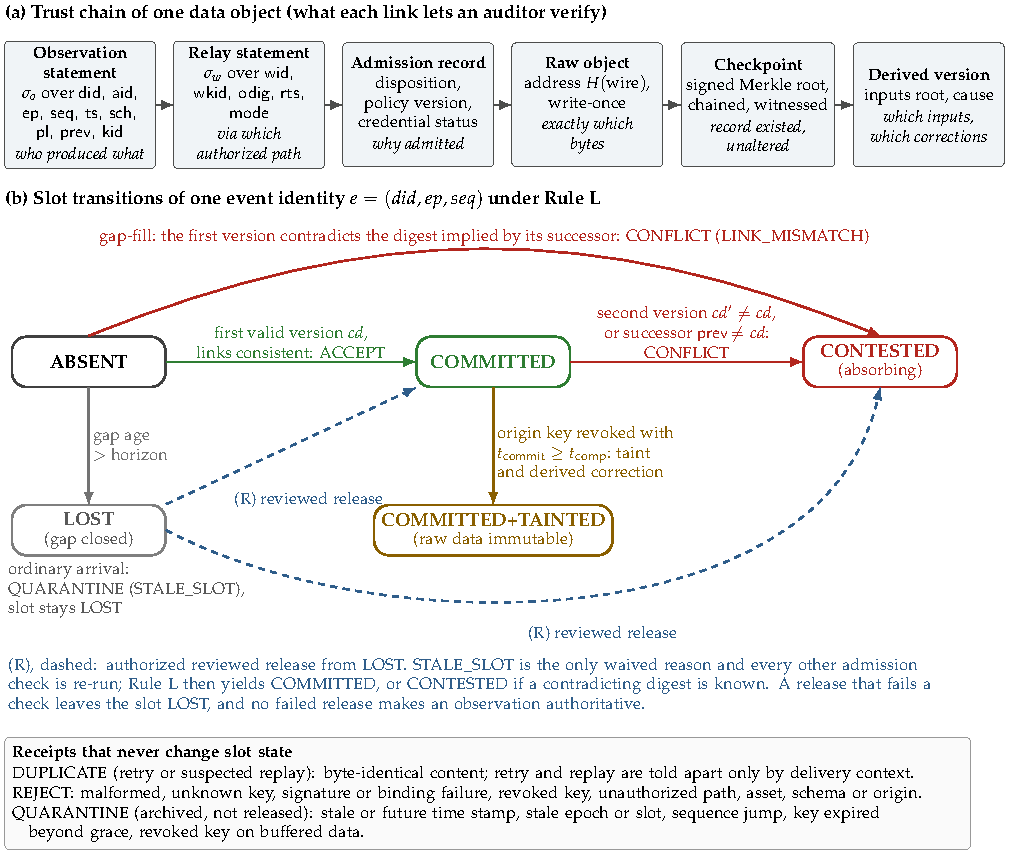
\includegraphics{figures/fig_chain_state.pdf}
\caption{(\textbf{a}) Trust chain of one data object and what each link lets an auditor verify: observation statement and relay statement (bound through \textsf{odig}), admission record, write-once raw object, signed and witnessed Merkle checkpoint, and derived version with its inputs and cause. (\textbf{b}) Event-identity slot transitions under Rule L: the state of a slot is a function of the admitted evidence set (ABSENT, COMMITTED, CONTESTED, LOST, and COMMITTED+TAINTED after revocation with a compromise time). Ordinary arrival at a LOST slot remains quarantined (STALE\_SLOT); an authorized reviewed release (dashed, R) may re-run admission with STALE\_SLOT as the only waived reason and reach COMMITTED or CONTESTED under Rule L, and a failed release creates no authoritative observation. The taint transition is subject to the reviewed-release conditions of Section~\Mref{sec:lifecycle} of the article (a slot released under the revoked key is exempt while its release condition holds under the current revocation record). Receipts that do not change slot state are listed below; Table~\ref{tab:S-transitions} specifies the complete transitions.\label{fig:S-state}}
\end{figure}

\begin{table}[!htbp]
\caption{Transitions of the event-identity slot machine (Current state + Evidence + Policy condition $\rightarrow$ Next state). Ordinary arrival transitions are distinguished from authorized review-release transitions (marked R). The default one-hour gap-closure horizon was not reached in the scenario campaigns; a regression test with a five-second horizon exercises LOST, STALE\_SLOT quarantine and reviewed release, and the bounded lifecycle check (Table~\ref{tab:S-bounded}) combines gap closure, release, revocation and rotation.\label{tab:S-transitions}}
\footnotesize
\begin{tabularx}{\linewidth}{@{}>{\raggedright\arraybackslash}p{1.95cm}>{\raggedright\arraybackslash}X>{\raggedright\arraybackslash}X>{\raggedright\arraybackslash}X@{}}
\toprule
Current & Evidence & Condition & Next (cause)\\
\midrule
ABSENT & first version $cd$; no implied digest or implied $=cd$ & admission checks passed & COMMITTED (ACCEPT)\\
ABSENT & first version $cd$; implied digest $\neq cd$ & admission checks passed & CONTESTED (LINK\_MISMATCH)\\
ABSENT & implied digest only (successor received) & -- & ABSENT, expected digest known\\
COMMITTED & second version $cd'\neq cd$ & admission checks passed & CONTESTED (EQUIVOCATION)\\
COMMITTED & successor with $\textsf{prev}\neq cd$ & successor admitted & CONTESTED (LINK\_MISMATCH)\\
COMMITTED & origin key revoked with $t_\mathrm{comp}\le t_\mathrm{commit}$ (also after a revised record with an earlier $t_\mathrm{comp}$) & revocation observed by verifier; for a slot released under the revoked key: its release condition fails under the current record & COMMITTED+TAINTED (REVOCATION)\\
ABSENT in open gap & gap age $>$ gap-closure horizon & periodic tick & LOST (GAP\_CLOSED)\\
CONTESTED & any further version & -- & CONTESTED (absorbing; evidence kept)\\
LOST & arriving version without an authorized waiver & ordinary admission & LOST (receipt QUARANTINE STALE\_SLOT)\\
LOST (R) & version re-evaluated through an authorized release & STALE\_SLOT is the only waived reason; all other admission checks pass & COMMITTED or CONTESTED under Rule L; on failure no authoritative observation (RELEASE\_FAILED)\\
ABSENT (R) & quarantined version (STALE\_TS, STALE\_EPOCH, REVOKED\_BUFFERED, \ldots) re-evaluated through an authorized release & only the case's reason waived; REVOKED\_BUFFERED also requires the release-evidence condition (discretionary: $ts<t_\mathrm{comp}$; witness: token for the exact digest before $t_\mathrm{low}$) & COMMITTED or CONTESTED under Rule L; a conflict records the version as evidence, nothing becomes authoritative\\
any & identical $cd$ already admitted & -- & unchanged (DUPLICATE RETRY or SUSPECTED\_REPLAY)\\
any & reject or quarantine condition (Algorithm 1) & -- & unchanged (REJECT / QUARANTINE)\\
\bottomrule
\end{tabularx}
\end{table}

\begin{table}[!htbp]
\caption{Invariants, their oracles and the scenarios that exercise them.\label{tab:S-invariants}}
\footnotesize
\begin{tabularx}{\linewidth}{lXX}
\toprule
\textbf{Invariant} & \textbf{Statement} & \textbf{Oracle (scenarios)}\\
\midrule
I1 Integrity & modifying any protected field without the key yields REJECT and no state change & unit test over all 18 protected fields; non-legitimate admissions (E2, E3, E6)\\
I2 Authorization & every committed slot has an ACCEPT record with PERMIT under the policy in force & registry audit; unauthorized-path admissions (E4, E15)\\
I3 Idempotency & at most one authoritative observation per identity & duplicate authoritative count (E7, E11)\\
I4 Non-overwrite & two validly signed contents for one identity are never authoritative & equivocation/gap-fill admissions (E5, E8)\\
I5 Provenance & latest derived versions reference only authoritative inputs; roots and aggregates recompute & lineage audit (all runs)\\
I6 Immutability & committed raw bytes and checkpointed evidence cannot change undetected & raw-store and evidence audits (E16)\\
I7 Credential enforcement and taint & ordinary admission after an observed revocation is refused or quarantined; an explicitly authorized release exception is audited separately; the selector taints origin-key commits at or after $t_\mathrm{comp}$ (commit time, not proof of creation time; re-run on revised records) & E14 ordinary-admission and taint counts; release-then-taint regressions and the lifecycle analysis (Table~\ref{tab:S-a5})\\
I8 Recovery & buffered observations within horizon committed exactly once (a suspected-replay label may occur but is non-authoritative) & missing and duplicate counts (E11)\\
I9 Convergence & for a fixed admitted evidence set, final state independent of delivery order & permutation unit test; exact windows (E9, E10)\\
I10 Determinism & replaying the receipt log reproduces every disposition and the registry & decision-replay audit (all runs)\\
\bottomrule
\end{tabularx}
\end{table}

\noindent\textbf{Locality of Rule L: statement, proof, exclusions and liveness.} The model has identities $e=(d,p,q)$ with predecessor $\mathrm{pred}(e)=(d,p,q-1)$ for $q>0$ and none for $q=0$; an admitted statement $s$ has identity $e(s)$, content digest $cd(s)$ and link $\mathrm{prev}(s)$, a digest or $\bot$. The evidence state is $E=(V,I)$, and admission updates $V(e(s))\leftarrow V(e(s))\cup\{cd(s)\}$ and, if $q(e(s))>0$ and $\mathrm{prev}(s)\neq\bot$, $I(\mathrm{pred}(e(s)))\leftarrow I(\mathrm{pred}(e(s)))\cup\{\mathrm{prev}(s)\}$; in the implementation these are the only writes to $V$ and $I$ (\texttt{PBTIVerifier.\_\allowbreak{}history} and the \texttt{\_\allowbreak{}history} methods of the historical and the corrected B5 subclass, which perform the same two writes). An \emph{admission} is a receipt that reaches the write to $V$: for \sys\ these are the ACCEPT and CONFLICT receipts and the re-run admission of a reviewed release; for B5 they also include the FEED\_FORK\_HOLD receipts, which write $V$ and $I$ before the hold. Classes: ABSENT if $V(e)=\emptyset$; otherwise COMMITTED if $|V(e)\cup I(e)|=1$ and CONTESTED if $|V(e)\cup I(e)|\ge 2$; LOST if the gap-closure flag $\lambda(e)$ is set; authority requires COMMITTED and no taint flag $\tau(e)$, and for B5 additionally that $e$ is not held. \emph{Lemma}: for any $E$ and any sequence $S$ of $k$ admitted statements with no lifecycle transition in between, $E'$ differs from $E$ only on $A(S)=\{e(s_i)\}\cup\{\mathrm{pred}(e(s_i)): q(e(s_i))>0,\ \mathrm{prev}(s_i)\neq\bot\}$, and $|A(S)|\le 2k$, with equality only when the $2k$ identities are pairwise distinct. \emph{Proof sketch}: by induction on $k$, since each update writes $V$ at one identity and $I$ at most at one other; the class of $e\notin A(S)$ is a function of $V(e)$, $I(e)$ and $\lambda(e)$ and its authority in addition of $\tau(e)$, and $\lambda$ and $\tau$ are written only by gap closure and revocation processing, which are excluded. The number of identities whose class changes can reach $2k$ but is not implied by pairwise distinct identities alone. \emph{Exclusions}: (E1) admission decisions that earlier admissions or time change (epochs, gaps, sequence jumps, horizons, key validity, revocation, policy versions); (E2) lifecycle transitions (gap closure marks a range LOST; revocation taints every qualifying commit of a key); (E3) downstream dependency fan-out; (E4) undetected contamination (a forged version for which no contradiction is admitted stays COMMITTED); (E5) the selective-hold extension, whose authority depends on feed-level suspicion; (E6) replicated verifiers. \emph{Liveness, separate from this safety property}: (L1) a gap-fill or equivocating version is contested only if a contradictory version or successor link is admitted within the freshness, gap and epoch horizons; (L2) a quarantined or held observation is released only if a reviewer runs and the release evidence its policy requires is available; (L3) retroactive containment requires a published and processed revocation with $t_\mathrm{comp}$, and its precision depends on how accurately $t_\mathrm{comp}$ is known. The proof is a pen-and-paper argument (repository \texttt{formal/\allowbreak{}LOCALITY\_\allowbreak{}PROOF.md}); it has not been machine-checked, and a checklist for its review is in the repository (\texttt{formal/\allowbreak{}PROOF\_\allowbreak{}REVIEW\_\allowbreak{}CHECKLIST.md}). An AI-performed audit of the argument found it correct but imprecise in the points corrected above, and an exhaustive checker that the same AI system wrote from the statement alone, without the verifier code, found no violation in $4.07\times10^{9}$ (state, batch) cases of the pure model and in 1{,}000 random histories (10{,}803 signed receipts) on the real verifier.

\begin{table}[!htbp]
\caption{Bounded checks of Rule L and of the lifecycle (repository \texttt{results/\allowbreak{}v4/\allowbreak{}formal/\allowbreak{}v4\_\allowbreak{}locality\_\allowbreak{}lifecycle\_\allowbreak{}check.json}; \WAfourAllPass). These are bounded results, not proofs. An earlier bounded check examined Rule L \VFormalSummary.\label{tab:S-bounded}}
\footnotesize
\begin{tabularx}{\linewidth}{lXr}
\toprule
\textbf{Part} & \textbf{Scope and properties} & \textbf{Cases}\\
\midrule
M (model) & implementation-independent model of $(V,I)$; every base set of two universes (one epoch, sequence 0--2, two contents, prev $\in\{G,F,\bot\}$: 14 statements; two epochs, sequence 0--1: 12 statements) and every batch of one or two further statements: changed classes $\subseteq A(S)$, $|A(S)|\le 2|S|$, both orders equal, contest absorbing & \WAfourMcases\\
L (implementation) & unmodified verifier, real Ed25519 signatures: every base set of the two-epoch universe with every single further statement & \WAfourLexhaustive\\
L (sample) & seeded random batches of two or three statements over both universes & \WAfourLrandom\\
C (lifecycle) & every operation sequence of length $\le 4$ over 13 operations (deliveries over two epochs including a forged alternative and a rotated-key statement; gap closure; revocation with early or late $t_\mathrm{comp}$; release with fresh or stale snapshot; rejection): evidence conformance, absorbing contest, authority and derived data, taint exactness, no ordinary admission under a revoked key, release safety, stale-snapshot refusal, per-delivery locality, rotation grace & \WAfourCexhaustive\\
C (sample) & seeded random sequences of length 5--8 & \WAfourCrandom\\
C (both rows) & operations exercised over all lifecycle sequences: \WAfourCops; releases \WAfourCreleased; stale-snapshot refusals \WAfourCstale & \\
\bottomrule
\end{tabularx}
\end{table}
\noindent The lifecycle check found one defect before the confirmatory runs: after a revocation record was revised with an earlier compromise time, the verifier did not re-run the taint selector, so an observation committed after the revised compromise time stayed authoritative (minimal schedule: commit at 2~s; revoke with $t_\mathrm{comp}=3$~s; revise to $t_\mathrm{comp}=0$). The fix keeps a key revoked from its first revocation, lets a revision only move $t_\mathrm{comp}$ earlier and re-runs the selector; a record released under a revoked key stays exempt only while its release condition holds. The counterexample is kept in the repository. No scenario revokes a key twice, and the re-executed main evaluation was identical on the corrected source. The symbolic model (ProVerif 2.05; Dolev--Yao attacker, unbounded sessions, adaptive key compromise) establishes the signature-binding correspondences stated in the article; its variant with an attacker-writable device-to-gateway link shows that the device key alone then suffices. Rego parity: \VParityWellFormedExact\ of \VParityWellFormedN\ well-formed and \VParityMalformedReqExact\ of \VParityMalformedReqN\ malformed requests gave the same decision and reason in the Python decision point and in the Rego policy evaluated by rego-cpp; OPA itself was not run.

\section{Environment, Evaluation Stages, Evidence Levels and Reproduction}\label{sec:S-env}
\begin{table}[!htbp]
\caption{Execution environment recorded in the result manifests. Source digest: SHA-256 over the files in \texttt{src/\allowbreak{}} as recorded by each campaign; repository file names of the runs are given in \texttt{typewriter}. The Rego parity harness used regopy 1.5.2 (rego-cpp 1.5.2); the SQLite library version of the wall-clock runs was not recorded in their manifests. ``Final'' refers to the main-evaluation and performance campaigns; the review-schedule, selective-hold and re-execution campaigns recorded source digest \texttt{8dfae6decd80\ldots} in their manifests (platform kernel 6.18.44, Python 3.13.18; Tables~\ref{tab:S-stages} and~\ref{tab:S-reexec}).\label{tab:S-env}}
\footnotesize\centering
\begin{tabular}{p{4.1cm}p{11.4cm}}
\toprule
Item & Value\\
\midrule
CPU & \texttt{Intel(R) Xeon(R) Processor @ 2.10GHz}\\
Logical CPUs / RAM & \texttt{2 / 7.84 GB}\\
Python & \texttt{3.13.18}\\
cryptography / NumPy / SciPy / pandas & \texttt{50.0.1 / 2.5.3 / 1.18.1 / 3.0.5}\\
Platform & \texttt{Linux-6.18.44-fc-v230-x86\_64-with-glibc2.39 (ablations (seeds 1--10); ablations (seeds 11--20); audit; end-to-end; revocation (seeds 1--10); revocation (seeds 11--20); scenarios (seeds 1--10); scenarios (seeds 11--20); throughput; scaling)}\\
Platform & \texttt{Linux-6.18.44-fc-v233-x86\_64-with-glibc2.39 (B4 mixed workload (seeds 1--20); B4 scenarios (seeds 1--20); v3\_audit\_rerun; v3\_batching; v3\_factorial; v3\_mixed\_b5 (B5 rows); v3\_mixed\_b5 (B5S rows); v3\_mixed\_b5 (PBTI-R rows); v3\_mixed\_b5\_fixedB5; v3\_mixed\_b5s\_fixed; v3\_mqtt\_e2e; v3\_mqtt\_e2e\_skab; v3\_replay\_skab; v3\_scenarios\_b5 (B5 rows); v3\_scenarios\_b5 (B5S rows); v3\_scenarios\_b5\_fixedB5; v3\_scenarios\_b5s\_fixed; v3\_scenarios\_pbtir; v3\_sweep)}\\
Source digest 0c21cbd40d64\ldots & \texttt{v3\_mixed\_b5 (PBTI-R rows); v3\_scenarios\_pbtir}\\
Source digest 1fc3ae032b24\ldots & \texttt{ablations (seeds 1--10); ablations (seeds 11--20); audit; end-to-end; revocation (seeds 1--10); revocation (seeds 11--20); scenarios (seeds 11--20); throughput; scaling}\\
Source digest 2cf3f17f3f6e\ldots & \texttt{scenarios (seeds 1--10)}\\
Source digest 7a711eb89ec8\ldots & \texttt{B4 mixed workload (seeds 1--20); B4 scenarios (seeds 1--20)}\\
Source digest c6305c988647\ldots & \texttt{v3\_factorial; v3\_mixed\_b5 (B5 rows); v3\_mixed\_b5 (B5S rows); v3\_mixed\_b5\_fixedB5; v3\_mixed\_b5s\_fixed; v3\_scenarios\_b5 (B5 rows); v3\_scenarios\_b5 (B5S rows); v3\_scenarios\_b5\_fixedB5; v3\_scenarios\_b5s\_fixed; v3\_sweep}\\
Source digest dd8dcd908d82\ldots & \texttt{v3\_audit\_rerun; v3\_batching; v3\_mqtt\_e2e; v3\_mqtt\_e2e\_skab; v3\_replay\_skab}\\
Regression check & \texttt{114 stored specifications (64 earlier scenario runs, 50 feed-level extension runs) re-run under the current source: 0 differences (results/summary/regression\_check\_v3.json)}\\
Broker / MQTT client & \texttt{mosquitto version 2.0.18 / paho-mqtt 2.1.0}\\
\bottomrule
\end{tabular}
\end{table}

\begin{table}[!htbp]
\caption{Evaluation stages of the article, their design, registration and evidence levels (summarized in Section~\Mref{sec:design} of the article). Levels: A, confirmatory and registered in advance (self-recorded); B, exploratory or descriptive; C, amendment-informed; D, formal or deterministic verification; E, performance on one host (no device or multi-host measurement). Repository identifiers, configurations and seeds: Table~\ref{tab:S-stages}.\label{tab:S-levels}}
\footnotesize
\begin{tabularx}{\linewidth}{>{\raggedright\arraybackslash}p{2.9cm}>{\raggedright\arraybackslash}X>{\raggedright\arraybackslash}p{4.6cm}>{\raggedright\arraybackslash}p{3.1cm}>{\raggedright\arraybackslash}p{1.3cm}}
\toprule
\textbf{Stage} & \textbf{Question} & \textbf{Design} & \textbf{Registration} & \textbf{Level}\\
\midrule
Main evaluation & Which pipelines admit forged or lose legitimate data? & E1--E15, eight pipelines, seeds 1--20 (\RScenarioRuns\ + \VXOneRuns\ runs) & P1--P3 for B5 and B5s; P4 (B4) describes stored runs; B1--B4 comparisons not registered & A (P1--P3), B\\
Mixed workload & All classes at once & 16th workload, seeds 1--20 (\VMixRuns\ runs) & exploratory & B\\
Re-execution with time-dependent outcomes & Are stored results reproducible; what do final counts conceal? & main evaluation and mixed workload re-run with the tracer (\XRunsReexec\ runs) & replication gate of the second registration & B\\
Review-schedule evaluation & Does the availability difference survive faster or matched review? & E5, E8, E11b, mixed; \sys\ and 21 B5/PBTI-R schedule arms; seeds 21--40 (\XRunsReview\ runs) & H1a--H1d; gates G1, G2 & A\\
Selective-hold grid & Do targeted holds reduce retained forgeries? & equivocation $\times$ suppression grid, delayed successors, suppression runs; 7 arms; seeds 21--40 (\XRunsGrid\ runs) & H3a--H3c; gates G3, G4 & A\\
Selective-hold factorial cells & Same, where feed-level review retained fewer forgeries & eight factorial cells, 7 arms, seeds 21--40 (\XRunsCells\ runs) & amendment; gates G3F, G4F & C\\
Selective-hold controls & Side effects in every workload & 16 workloads, seeds 1--20 (\XRunsControls\ runs) & descriptive & B\\
Sensitivity analyses & Dependence on stressor rates & 11-factor sweep at 0--20\%, $2^{7-3}_\mathrm{IV}$ factorial; seeds 1--20 (\VSweepRuns\ + \VFactRuns\ runs) & registered as descriptive & B\\
Public-telemetry replay & Real sensor dynamics & SKAB at 1, 5, 10$\times$, seeds 1--20 (\VRpRuns\ runs) & exploratory & B\\
Corrected-comparator reruns & Do the results depend on the known B5 defects? & every B5 and B5s specification of all stages above, original seeds (\YRunsRerun\ runs) & registered outcomes, families, margins and gates applied unchanged; correction decided after the results (DV8) & that of the rerun stage\\
Attacker-model robustness & How much do the results depend on the attack generator? & mixed workload with a consistent impersonator; \sys, PBTI-R, B5 (one-shot and event-driven); seeds 21--40 (\YEfourRunsN\ runs) & not registered (DV9) & B\\
Control traces & Which failure modes are common to all rules? & six deterministic traces, four pipelines & not registered & D\\
Lifecycle analysis & Which evidence justifies release under a revoked key? & \WAfiveRows\ deterministic timelines (11 cases, 3 policies, 2 pipelines) & not registered & D\\
Formal properties & Locality and signature bindings & proof, symbolic model, bounded enumeration & --- & D\\
Performance & Processing, size and latency costs & in-process, batching, MQTT/TLS on one host & descriptive & E\\
\bottomrule
\end{tabularx}
\end{table}

\begin{table}[!htbp]
\caption{Evaluation stages of the article and their repository identifiers, configurations, seeds and run counts. All paths are relative to the repository root.\label{tab:S-stages}}
\footnotesize
\begin{tabularx}{\linewidth}{p{3.0cm}p{4.4cm}Xp{1.5cm}}
\toprule
\textbf{Stage (article)} & \textbf{Raw results} & \textbf{Configuration or command; registration} & \textbf{Seeds; runs}\\
\midrule
Main evaluation, B1--B4 and \sys & \texttt{results/\allowbreak{}raw/\allowbreak{}scenarios*.jsonl}, \texttt{ablations*.jsonl}, \texttt{revocation*.jsonl}, \texttt{audit.jsonl} & \texttt{experiments/\allowbreak{}run\_\allowbreak{}campaign.py} (\texttt{make campaign}); not registered & 1--20; \RScenarioRuns\ scenario runs\\
Main evaluation, B5, B5s, PBTI-R & \texttt{results/\allowbreak{}raw/\allowbreak{}v3\_\allowbreak{}scenarios\_\allowbreak{}b5*.jsonl}, \texttt{v3\_\allowbreak{}scenarios\_\allowbreak{}pbtir.jsonl} & \texttt{make campaign-v3}; first registration \texttt{research/\allowbreak{}V3/\allowbreak{}PREREGISTRATION.md} & 1--20; \VXOneRuns\\
Mixed workload & \texttt{results/\allowbreak{}raw/\allowbreak{}v3\_\allowbreak{}mixed\_\allowbreak{}b5*.jsonl} & as above; exploratory & 1--20; \VMixRuns\\
Re-execution with time-dependent outcomes & \texttt{results/\allowbreak{}v4/\allowbreak{}raw/\allowbreak{}A0\_\allowbreak{}core.jsonl}; \texttt{results/\allowbreak{}v4/\allowbreak{}summary/\allowbreak{}A0\_\allowbreak{}comparison.json} & \texttt{experiments/\allowbreak{}v4\_\allowbreak{}configs/\allowbreak{}A0\_\allowbreak{}core.json}; replication gate of the second registration & 1--20; \XRunsReexec\\
Review-schedule evaluation & \texttt{results/\allowbreak{}v4/\allowbreak{}raw/\allowbreak{}A1\_\allowbreak{}review.jsonl} & \texttt{experiments/\allowbreak{}v4\_\allowbreak{}configs/\allowbreak{}A1\_\allowbreak{}review.json}; second registration \texttt{research/\allowbreak{}V4/\allowbreak{}PREREGISTRATION\_\allowbreak{}V4.md} & 21--40; \XRunsReview\\
Selective-hold grid & \texttt{results/\allowbreak{}v4/\allowbreak{}raw/\allowbreak{}A3\_\allowbreak{}selective.jsonl} & \texttt{experiments/\allowbreak{}v4\_\allowbreak{}configs/\allowbreak{}A3\_\allowbreak{}selective.json}; second registration & 21--40; \XRunsGrid\\
Selective-hold factorial cells & \texttt{results/\allowbreak{}v4/\allowbreak{}raw/\allowbreak{}A3\_\allowbreak{}factorial.jsonl} & \texttt{experiments/\allowbreak{}v4\_\allowbreak{}configs/\allowbreak{}amendment1/\allowbreak{}A3\_\allowbreak{}factorial.json}; amendment \texttt{research/\allowbreak{}V4/\allowbreak{}PREREGISTRATION\_\allowbreak{}V4\_\allowbreak{}AMENDMENT\_\allowbreak{}1.md} & 21--40; \XRunsCells\\
Selective-hold controls & \texttt{results/\allowbreak{}v4/\allowbreak{}raw/\allowbreak{}A3\_\allowbreak{}scenarios.jsonl} & \texttt{experiments/\allowbreak{}v4\_\allowbreak{}configs/\allowbreak{}A3\_\allowbreak{}scenarios.json}; descriptive & 1--20; \XRunsControls\\
Sensitivity analyses & \texttt{results/\allowbreak{}raw/\allowbreak{}v3\_\allowbreak{}sweep.jsonl}, \texttt{v3\_\allowbreak{}factorial.jsonl} & \texttt{make campaign-v3}; registered as descriptive & 1--20; \VSweepRuns, \VFactRuns\\
Public-telemetry replay & \texttt{results/\allowbreak{}raw/\allowbreak{}v3\_\allowbreak{}replay\_\allowbreak{}skab.jsonl} & \texttt{make campaign-v3} with \texttt{SKAB\_\allowbreak{}DIR}; exploratory & 1--20; \VRpRuns\\
Lifecycle analysis & \texttt{results/\allowbreak{}v4/\allowbreak{}summary/\allowbreak{}A5\_\allowbreak{}lifecycle\_\allowbreak{}matrix.json} & \texttt{scripts/\allowbreak{}a5\_\allowbreak{}lifecycle\_\allowbreak{}matrix.py}; not registered & --; \WAfiveRows\ rows\\
Bounded checks & \texttt{results/\allowbreak{}v4/\allowbreak{}formal/\allowbreak{}}, \texttt{results/\allowbreak{}formal/\allowbreak{}} & \texttt{formal/\allowbreak{}v4\_\allowbreak{}locality\_\allowbreak{}lifecycle\_\allowbreak{}check.py}, \texttt{formal/\allowbreak{}rule\_\allowbreak{}l\_\allowbreak{}bounded\_\allowbreak{}check.py}, \texttt{formal/\allowbreak{}*.pv} & --\\
Performance & \texttt{results/\allowbreak{}raw/\allowbreak{}throughput*.jsonl}, \texttt{mqtt\_\allowbreak{}e2e.jsonl}, \texttt{v3\_\allowbreak{}batching.jsonl}, \texttt{v3\_\allowbreak{}mqtt\_\allowbreak{}e2e*.jsonl} & \texttt{make perf}, \texttt{make perf-v3}, \texttt{make e2e}, \texttt{make e2e-v3} & repetitions in Tables~\ref{tab:S-throughput}--\ref{tab:S-e2e-skab}\\
Second-environment re-execution & \texttt{results/\allowbreak{}v7/\allowbreak{}reexec\_\allowbreak{}cloud/\allowbreak{}} & \texttt{tools/\allowbreak{}reexec/\allowbreak{}reproduce\_\allowbreak{}subset.sh} (Table~\ref{tab:S-reexec}) & subsets; Table~\ref{tab:S-reexec}\\
Corrected-comparator reruns & \texttt{results/\allowbreak{}v9/\allowbreak{}raw/\allowbreak{}*\_\allowbreak{}B5c.jsonl}, \texttt{*\_\allowbreak{}B5Sc.jsonl} & \texttt{experiments/\allowbreak{}v9/\allowbreak{}run\_\allowbreak{}all\_\allowbreak{}b5c.sh}; frozen configurations; analysis \texttt{tools/\allowbreak{}v9/\allowbreak{}build\_\allowbreak{}corrected\_\allowbreak{}results.sh} & as the stages; \YRunsRerun\\
Attacker-model robustness and controls & \texttt{results/\allowbreak{}v9/\allowbreak{}raw/\allowbreak{}attacker\_\allowbreak{}consistent\_\allowbreak{}impersonator.jsonl}, \texttt{attacker\_\allowbreak{}controls.json} & \texttt{experiments/\allowbreak{}v9/\allowbreak{}run\_\allowbreak{}attacker\_\allowbreak{}consistent.py}, \texttt{attacker\_\allowbreak{}controls.py} & 21--40; \YEfourRunsN\\
Reference-model check of the corrected B5 & \texttt{results/\allowbreak{}v9/\allowbreak{}b5c\_\allowbreak{}refmodel/\allowbreak{}} & \texttt{tools/\allowbreak{}v9/\allowbreak{}b5c\_\allowbreak{}refmodel\_\allowbreak{}campaign.sh} & generator seeds; \YRefN\ comparisons\\
\bottomrule
\end{tabularx}
\end{table}

\begin{table}[!htbp]
\caption{Principal findings of the article and their evidence levels (levels as in Table~\ref{tab:S-levels}).\label{tab:S-findings}}
\footnotesize
\begin{tabularx}{\linewidth}{>{\raggedright\arraybackslash}X>{\raggedright\arraybackslash}p{1.6cm}>{\raggedright\arraybackslash}p{4.0cm}}
\toprule
\textbf{Finding} & \textbf{Level} & \textbf{Evidence}\\
\midrule
Final forged admissions are identical for per-identity and feed-level containment in all 15 scenarios and in the four confirmatory workloads under every review schedule (by construction the feed-level comparator can only be lower than PBTI-R with the same reviewer) & A & article Table~\Mref{tab:primary}; Table~\ref{tab:S-full}\\
Final losses are identical in \VOTwoBFiveIdentical\ of 15 scenarios; the exception is recovery of a beyond-horizon backlog by the reviewer, which PBTI-R matches & A & Table~\ref{tab:S-full}; article Section~\Mref{sec:res-main}\\
With one-shot 60/10~s review, feed-level containment withholds genuine data longer (E5: $+$\WAoneEfiveBFivehistvsPBTIWdshort~s per observation) but has less exposure in the mixed workload & A & article Table~\Mref{tab:effects}\\
With event-driven review, availability is equivalent in E5 and E8 and better for B5 in E11b and the mixed workload through recovery (gate G1 not met) & A & article Table~\Mref{tab:effects} and Figure~\Mref{fig:delay}\\
With matched review, final outcomes are identical or equivalent in every schedule and workload (gate G2); withholding differs with $R\ge 5$~s or 10~s cadence, and feed holds reduce exposure in the mixed workload unless review is event-driven & A & article Section~\Mref{sec:res-review}; Table~\ref{tab:S-a1-tests}\\
When equivocation coincides with suppressed messages, feed-level holds retain fewer forgeries than Rule L & B, C & article Section~\Mref{sec:res-selective}; Tables~\ref{tab:S-factorial} and~\ref{tab:S-a3f}\\
Selective holds remove those forgeries at a cost in genuine data; their registered grid gates failed & A (negative), C & article Section~\Mref{sec:res-selective}; Figure~\ref{fig:S-factorial}; Table~\ref{tab:S-gates}\\
A time-stamp condition for release under revoked keys admits backdated forgeries; an exact-content witness policy prevents them if the witness is trusted & D & article Section~\Mref{sec:res-release}; Table~\ref{tab:S-a5}\\
$k$ admitted statements change the class and authority of at most $2k$ identities when no lifecycle transition intervenes (proof sketch; bounded checks) & D & article Proposition~\Mref{prop:locality}; Table~\ref{tab:S-bounded}\\
Most of $W$ in E5 and in the factorial cells is end-of-run loss (observations still missing at the horizon); the extra withholding of the feed-level comparator is delay & B (exploratory) & article Section~\Mref{sec:primary}; Table~\ref{tab:S-v9-wsplit}\\
With a consistent impersonator every pipeline retains far more forgeries than with the registered one; one-shot feed holds still expose less and withhold more, and event-driven B5 and PBTI-R stay close & B (exploratory) & article Section~\Mref{sec:res-attacker}; Tables~\ref{tab:S-v9-e04}--\ref{tab:S-v9-controls}\\
Correcting the comparator's known defects changed no registered class, claim gate or prediction; it lowered B5's withholding and losses and raised its exposure slightly where its reviewer acts quickly or factorial stressors combine & that of the rerun stage (DV8) & article Section~\Mref{sec:impl}; Tables~\ref{tab:S-v9-runs} and~\ref{tab:S-v9-classes}\\
Throughput \RTpRatioBTwo$\times$ and message size \RWireRatioBTwo$\times$ of a Zero-Trust baseline; networked saturation between 1000 and 1250 messages/s on one host & E & article Section~\Mref{sec:res-perf}; Tables~\ref{tab:S-throughput} and~\ref{tab:S-e2e2}\\
\bottomrule
\end{tabularx}
\end{table}

\begin{table}[!htbp]
\caption{Registration chronology, amendments and deviations. All plans are self-recorded in the repository with SHA-256 hashes and times written by the executing process; they were not deposited with an external registry, so a hash attests that a file is unchanged, not when it was written.\label{tab:S-chronology}}
\footnotesize
\begin{tabularx}{\linewidth}{p{3.2cm}p{2.9cm}X}
\toprule
\textbf{Record} & \textbf{Recorded (self-reported)} & \textbf{Content and effect}\\
\midrule
First registration (\texttt{research/\allowbreak{}V3/\allowbreak{}PREREGISTRATION.md}, SHA-256 \texttt{91f6b544\ldots}) & 3 Nov 2026, 22:51 UTC$-$6 & outcomes O1, O2; predictions P1--P4; decision rules for comparative wording; written before any feed-level, sweep, release-workflow, batching or new end-to-end result existed\\
Amendments 1--3 to the first registration & 3 Nov 2026, 23:26 UTC$-$6, before any campaign result was read & exploratory PBTI-R arm; full audits on seeds 1--5; 120~s production phase in the sensitivity analyses; no test or prediction changed\\
Amendment 4 to the first registration & 4 Nov 2026, 01:06 UTC$-$6 & B5 implementation fix after an audit failure in 2 of 20 mixed-workload runs, and re-run of every B5 and B5s arm; no test or prediction changed\\
Second registration (\texttt{research/\allowbreak{}V4/\allowbreak{}PREREGISTRATION\_\allowbreak{}V4.md}, SHA-256 \texttt{9d3247ff\ldots}, with the source and configuration hashes) & 5 Nov 2026, 05:39 UTC, before any run on seeds 21--40 & hypotheses H1a--H1d, H3a--H3c; outcomes; families; margins; classification rules; gates G1--G4; replication gate\\
Amendment to the second registration (SHA-256 \texttt{ac7945bb\ldots}) & 5 Nov 2026, 05:42 UTC, before any confirmatory selective-hold run & eight factorial cells with equivocation high and gates G3F, G4F; motivated by a one-seed pilot (seed 101) with retained forgeries at one grid point; data dependence disclosed\\
Deviation DV1 & during the re-execution & host restart after 318 of 1{,}320 runs; resumed with the frozen runner; no effect expected (deterministic runs)\\
Deviation DV2 & during the campaigns & campaigns run in a changed order; frozen source and configurations verified unchanged\\
Deviation DV3 & after the results & descriptive summaries of the selective-hold grid added; no test, class, family, margin or gate changed\\
Deviation DV4 & before the amendment & the selective-hold pilot was inspected beyond its error status, which led to the amendment\\
Deviation DV5 & analysis & the re-execution comparison also excludes audit-outcome fields (reported separately) and two runner labels\\
Deviation DV6 (found by the post-hoc audit) & analysis & the review-schedule Holm families contain 16 tests the hypotheses do not name (H1a on O2; H1b on O1, O2 and NLX), so the families of O1 and NLX have 84 instead of 80 tests and that of O2 48 instead of 40; conservative; with the families of the text no class or significance changes\\
Deviation DV7 (found by the post-hoc audit) & analysis & the bootstrap generator is seeded with 20261104 and the CRC32 checksum of each comparison's key, a derivation the plan does not state; it changes intervals only by Monte-Carlo error, and one resampling-dependent class results (Table~\ref{tab:S-gates})\\
Timing (found by the post-hoc audit) & 3--4 Nov 2026 & the first registration was written after the B1--B4 comparisons with \sys\ had been run (B4 scenario runs started at 17:57 UTC$-$6), so P4 describes stored runs and is reported as descriptive; B5 and its reviewer were debugged in smoke runs on seed 1, which the main evaluation also uses; amendments 1--3 were recorded at 23:26, eight minutes after the campaigns they govern were launched and before any result was read; the re-run with the corrected B5 started at 01:00, six minutes before amendment 4 was recorded\\
Timing (found by the post-hoc audit) & 5 Nov 2026 & the second registration records single-seed development values that already showed event-driven B5 close to \sys\ in E5; the factorial cells of the amendment ran before the registered grid (DV2); the amendment allows presenting PBTI-SH as useful if either G4 or G4F holds\\
Deviation (found by the post-hoc audit) & analysis & the first registration says that pairs identical in every seed are not tested; the analysis enters them into the Holm correction with $p=1$ (conservative)\\
Deviation DV8 & 6 Nov 2026, after all results above & B5 corrected in a separate module (\texttt{src/\allowbreak{}pbti/\allowbreak{}b5\_\allowbreak{}corrected.py}; historical module unchanged) after the audit had found its defects; every B5 and B5s specification rerun on its original seeds and analysed with the unchanged scripts; the article's principal results use the corrected comparator, the historical results are kept\\
Deviation DV9 & 6 Nov 2026, after all results above & exploratory attacker-model campaign (consistent impersonator, seeds 21--40) and control traces added; not registered, classes descriptive\\
Note (found by the post-hoc audit) & analysis & the analysis script that classifies the comparisons was not among the hash-frozen files; an AI-performed re-implementation written from the plan text reproduced 1180 of the 1182 classes, the other two (one grid point) depend on bootstrap resampling, and with the seeding of DV7 all 1182 were reproduced exactly\\
\bottomrule
\end{tabularx}
\end{table}

\noindent\textbf{Re-execution checks.} The re-execution of the main evaluation and the mixed workload under the extended source compared every stored run field by field: \WAzeroIdentical\ of \WAzeroCompared\ runs were identical over \WAzeroFieldComparisons\ field comparisons (wall-clock and audit timings, audit outcomes reported separately, and two runner labels excluded). The second re-execution ran the published commands of the minimal reproduction kit (\texttt{tools/\allowbreak{}reexec/\allowbreak{}reproduce\_\allowbreak{}subset.sh}) in a separate cloud environment, on a fresh copy of the repository, and compared every field except wall-clock timing with the stored rows (Table~\ref{tab:S-reexec}). Both re-executions were run by the same automated process that produced the results, so they show determinism and portability, not independent reproduction. The kit records date, hardware, operating system, package versions, git commit, source and configuration hashes, exact commands, seeds, exit codes and test counts, and is intended to be run by the authors on their own machines. In the second re-execution (\XRxDate; \XRxCpus\ vCPUs, \XRxOS, Python \XRxPython) the runner recorded the same source digest (\texttt{8dfae6decd80\ldots}) and configuration digests as the stored confirmatory campaigns.
\begin{table}[!htbp]
\caption{Second-environment re-execution of selected seeds (all fields compared except wall-clock timing: fields containing \texttt{\_\allowbreak{}us}, \texttt{wall\_\allowbreak{}s}, \texttt{audit\_\allowbreak{}static\_\allowbreak{}s}, \texttt{audit\_\allowbreak{}replay\_\allowbreak{}s}).\label{tab:S-reexec}}
\footnotesize\centering
% AUTO-GENERATED by tools/v7/analysis_v7.py -- do not edit by hand
\begin{tabular}{@{}lllrrrr@{}}\toprule
Stage & Seeds & Runs & Identical & Different & Errors & Field comparisons \\ \midrule
Main evaluation and mixed workload (re-executed) & 1, 2 & 132 & 132 & 0 & 0 & 12{,}367 \\
Review-schedule evaluation & 21, 22 & 176 & 176 & 0 & 0 & 19{,}550 \\
Selective-hold grid & 21, 22 & 294 & 294 & 0 & 0 & 29{,}687 \\
Selective-hold controls & 1, 2 & 40 & 40 & 0 & 0 & 3{,}995 \\
Selective-hold factorial cells & 21, 22 & 112 & 112 & 0 & 0 & 12{,}282 \\
\midrule
Lifecycle analysis (all rows) & -- & 68 & 68 & 0 & -- & -- \\
Bounded checks (all parts) & -- & -- & yes & -- & -- & -- \\
Test suite & -- & -- & \multicolumn{4}{l}{187 passed, 1 skipped, 0 failed} \\
\bottomrule\end{tabular}

\end{table}

\noindent\textbf{AI-performed checks.} Separate instances of the AI model used for this study, each given the specification, the repository and a narrow task but not the conclusions of the others, performed the following checks. None of them is a human review, and all instances share the training of the model that wrote the code, so errors common to that model would not be caught.
(i) \emph{Oracle and time-dependent outcomes.} Sixteen hand-computed traces drove the unmodified \sys, B5 and PBTI-SH verifiers, and an implementation of the outcome definitions that shares no code with the repository recomputed the primary outcomes of 20 re-run campaign runs (seeds 1, 2, 21 and 22 and one factorial cell) from its own record of the authoritative set; all 420 run-outcome values agreed with the stored rows, and seven consistency identities held in all 7540 stored rows. The check found two counter defects that affect only Table~\ref{tab:S-holds} and no primary outcome (caption of that table), and it showed that $W$ and NLX depend on the fixed 180~s drain: an observation that is never made available, and a forgery retained to the end, contribute until $T_\mathrm{end}$, so differences between pipelines that differ in end-of-run loss grow with the drain. An exploratory screen with drains 60~s and 120~s shorter (linear correction of the stored rows, which is exact when all losses and releases precede the shortened end; interval-based classes only, without Wilcoxon tests or Holm correction) changed the margin class of 25 of the 222 registered $W$ comparisons, all in the selective-hold analyses (Tables~\ref{tab:S-a3} and~\ref{tab:S-a3f}), and no gate outcome; in the grid, PBTI-SH's withholding was worse than \sys's beyond the margin at 4 points with the registered drain, at 2 with a 120~s drain and at none with a 60~s drain.
(ii) \emph{Statistics.} A re-implementation of the registered procedures written from the plan text recomputed all 1182 comparisons from the raw rows; Holm-adjusted significance agreed in all of them, and the classes as described in the note of Table~\ref{tab:S-chronology}; it also identified deviations DV6 and DV7.
(iii) \emph{Locality proof.} A line-by-line audit of the proof against the update rule and the verifier, an implementation-independent exhaustive model checker (4\,068\,762\,624 evidence-state and batch cases) and 1000 random histories (10\,803 receipts) on the unmodified verifier with real signatures found no counterexample; the audit led to the corrected statement of Proposition~\Mref{prop:locality} (hypothesis stated on the schedule, taint and gap-closure flags, reviewer decisions excluded) and to the wording ``proof sketch''.
(iv) \emph{Source code and the feed-level comparator.} A line-by-line audit of \sys, PBTI-R, PBTI-SH, B5, B5s, the simulator and the oracle against the specification documents, with a minimal reproduction of every suspicion and about 210 single runs of instrumented audit-only subclasses (the repository's classes were not edited), confirmed the Rule L slot states, duplicate handling, staleness checks, release waivers, reviewer checks and schedules, taint and revised revocations, the arm settings and the common random numbers (byte-identical receipt sequences across pipelines in two runs; identical per-label receipt counts in all 1300 campaign--cell--seed groups); the tracer matched the true authoritative set at 1247 mid-run checks. It found four minor defects. (a) B5 holds observations again that its reviewer had released, and can restart a fork after the feed resumed, when a late successor of an already contested slot arrives without new fork evidence; with this corrected in an audit-only subclass, B5's $W$ fell by up to 0.26~s per observation in single mixed-workload runs with periodic review and by at most 0.003~s with event-driven review, O1 and NLX did not change in those runs, and the two matched-review $W$ comparisons closest to the margin stayed worse beyond it (0.695 to 0.679~s and 0.699 to 0.690~s per observation); these single-run estimates of the audit are superseded by the complete reruns with the corrected implementation (\emph{Comparator correction} below). (b) When the reviewer releases a stale case of a held feed, B5 can keep the observation held without an open case (no occurrence in 66 instrumented mixed-workload runs). (c) The hold counter of Table~\ref{tab:S-holds} (see its caption). (d) A raw field counting distinct held observations misses holds made on arrival; it is not used. Defects (a) and (b) can disadvantage B5; all four were subsequently corrected in a separate implementation (\emph{Comparator correction} below). The audit also noted that B5's hold release does not re-run admission and that its resume rule keeps a forked feed held while the device produces (Section~\Mref{sec:pipelines} of the article), that under message loss the missing-message runs of the sensitivity factorial are not always consecutive (identically for every pipeline), and that an audit pass shows internal consistency and replayability rather than correctness against the specification, because decision replay runs the same code. A reference model of B5, written from the specification before any B5 code was read (frozen at 23:50 UTC on 5 November 2026) and compared with the real B5 in 39{,}600 synthetic comparisons and 26 instrumented scenario runs, matched the implementation exactly once six choices that the specification leaves open were restated; without them it matched 23{,}781 comparisons. These choices cut both ways: reviewing cases in identity order favours B5 and PBTI-R equally (with creation order the one-shot reviewer would have lost 175 observations in one E11b run), whereas re-forking from slot state and the absence of review cases for contested slots cost B5 at most 0.014~s per observation in $W$ and 0.0013 in AV5 on the real traces. The model confirmed defects (b) (no occurrence in 146 real runs) and (c) (hold counts 1--9\% too high with one-shot review and 14--38\% with event-driven review) and found no error of its own.

\noindent\textbf{Comparator correction.} Because the confirmatory comparisons set \sys\ against B5, the defects found by the audit were corrected rather than only described. The historical implementation (\texttt{src/\allowbreak{}pbti/\allowbreak{}b5.py}), which produced every frozen result and is listed in the freeze files, is unchanged; the corrected implementation is a separate module (\texttt{src/\allowbreak{}pbti/\allowbreak{}b5\_\allowbreak{}corrected.py}) with four changes. (C1) The feed-level response is triggered only by a receipt that adds new fork evidence: a second admitted version of its identity, an admitted successor link naming another digest for it, or a predecessor link naming none of the admitted versions of its predecessor; a successor that names one of the versions of an already contested predecessor no longer holds released observations again or restarts a hold after a resume. (C2) Every held committed observation has an open review case: a reviewed release of another reason whose re-run admission lands in a held feed continues as that observation's hold case (outcome \texttt{DEFERRED\_\allowbreak{}TO\_\allowbreak{}FEED\_\allowbreak{}HOLD}) instead of being closed without a case; a pending case of another reason for the same wire becomes the hold case; every hold is recorded as a slot-state change, which the event-driven review follows; and a hold case opened while a review decision is applied is decided from the next periodic pass on. (C3) Holds are counted once per transition, and distinct held and recovered observations are counted separately. (C4) The release of a tainted held observation is labelled as such. Identity order within a pass, the absence of review cases for contested identities with resume checked after each hold-case decision, and the event-driven candidate rule are kept; the six points that the specification had left open are now stated there (\texttt{docs/\allowbreak{}BASELINES.md}). \YRegTests\ regression tests reproduce each defect on the historical class and check the corrected behaviour, the kept choices and unchanged behaviour without fork evidence, and in \YRefN\ comparisons over the stream families of the reference model the corrected implementation matched the reference model with the corrected choices on the final authoritative set and every authority interval (\YRefEqual) and on the hold, fork and resume counters (\YRefCounters); it differed from the historical implementation in \YRefHistDiffers\ of these stress streams. Every B5 and B5s specification of the main evaluation, the mixed workload, the sweep, the factorial, the replay, the re-execution with the tracer, the review-schedule evaluation, the selective-hold grid and the factorial cells was rerun with the corrected implementation on its original seeds (\YRunsRerun\ of \YRunsAll\ runs); the frozen rows are kept, and the corrected rows are stored separately with the implementation identifier and the source digest. Historical runs without any fork evidence were reproduced in every outcome field (\YRowsNoforkIdentical\ of \YRowsNofork). The unchanged analysis scripts were then run on a tree in which only the B5 and B5s rows are replaced; outcome definitions, comparison families, margins and gates are those of the registrations. Table~\ref{tab:S-v9-runs} gives the run-level corrected-minus-original differences and Table~\ref{tab:S-v9-classes} the comparisons whose class changed; Data~S1 contains both versions of every per-cell table and comparison. The performance runs of B5 were not repeated: the in-process batching and worker study, whose disposition sequences equal those of \sys, and the end-to-end MQTT runs, in which every receipt was admitted, contain no fork evidence, so the correction cannot change their dispositions, but their timings were not re-measured with the corrected module. The lifecycle matrix (Table~\ref{tab:S-a5}) was recomputed with the corrected B5 and is unchanged (\YAfiveCorrectedDiffs\ differing rows).

\begin{table}[!htbp]
\caption{Corrected minus historical B5 and B5s, run by run on the same specifications and seeds. Changed: runs in which O1, O2, NLX, $W$ or AV5 differs; the other columns give the range of the differences over all runs of the stage (NLX, $W$ and AV5 only where the tracer ran). Counters (holds, distinct held and recovered observations) are not outcomes and are not counted here.\label{tab:S-v9-runs}}
\footnotesize\centering
\begin{tabularx}{\linewidth}{@{}>{\raggedright\arraybackslash}X lrrrrrrr@{}}
\toprule
Stage & Pipeline & Runs & Changed & $\Delta$O1 & $\Delta$O2 & $\Delta$NLX & $\Delta W$ (s) & $\Delta$AV5\\
\midrule
Main evaluation (15 scenarios, seeds 1--20) & B5 & 300 & 0 & 0 & 0 & -- & -- & --\\
Main evaluation (15 scenarios, seeds 1--20) & B5s & 300 & 0 & 0 & 0 & -- & -- & --\\
Mixed workload (seeds 1--20) & B5 & 20 & 0 & 0 & 0 & -- & -- & --\\
Mixed workload (seeds 1--20) & B5s & 20 & 0 & 0 & 0 & -- & -- & --\\
Stressor sweep & B5 & 940 & 0 & 0 & 0 & -- & -- & --\\
Sensitivity factorial & B5 & 320 & 31 & 0 & $-$4 to 0 & -- & -- & --\\
SKAB replay & B5 & 69 & 0 & 0 & 0 & -- & -- & --\\
Re-execution with the tracer & B5 & 320 & 0 & 0 & 0 & 0 & 0 & 0\\
Re-execution with the tracer & B5s & 320 & 0 & 0 & 0 & 0 & 0 & 0\\
Review-schedule evaluation (seeds 21--40) & B5 & 880 & 202 & 0 & $-$1 to 0 & 0.0 to 29.2 & $-$0.057 to 0.000 & 0.0000 to 0.0032\\
Selective-hold grid & B5 & 840 & 171 & 0 to 1 & $-$1 to 0 & 0.0 to 192.0 & $-$0.101 to 0.000 & 0.0000 to 0.0003\\
Selective-hold grid & B5s & 420 & 0 & 0 & 0 & 0 & 0 & 0\\
Selective-hold factorial cells & B5 & 320 & 184 & 0 to 1 & $-$5 to 0 & 0.0 to 154.8 & $-$0.289 to 0.000 & 0.0000 to 0.0014\\
Selective-hold factorial cells & B5s & 160 & 0 & 0 & 0 & 0 & 0 & 0\\
\bottomrule
\end{tabularx}

\end{table}

\begin{table}[!htbp]
\caption{Registered comparisons whose class differs between the historical and the corrected comparator (\YCmpClassChanged\ of \YCmpN\ comparisons of the review-schedule evaluation, the selective-hold grid and the factorial cells; \YCmpEstChanged\ estimates changed at all). Mean paired difference (arm $-$ reference) with 95\% bootstrap interval.\label{tab:S-v9-classes}}
\footnotesize\centering
\begin{tabularx}{\linewidth}{@{}llll>{\raggedright\arraybackslash}X>{\raggedright\arraybackslash}X@{}}
\toprule
Stage & Outcome & Cell & Comparison & Original: mean (95\% CI), class & Corrected: mean (95\% CI), class\\
\midrule
\multicolumn{6}{@{}l}{No comparison changed its class.}\\
\bottomrule
\end{tabularx}

\end{table}

\noindent\textbf{Attacker-model robustness campaign.} The consistent impersonator of the earlier five-seed check (\emph{Exploratory analyses} below; \texttt{experiments/\allowbreak{}v9/\allowbreak{}consistent\_\allowbreak{}impersonator.py}, the same logic moved into an importable module) was run on all 20 seeds 21--40 of the mixed workload of the review-schedule evaluation, for \sys, PBTI-R and B5 with one-shot ($R=60$~s, $C=10$~s) and event-driven review, B5 in its corrected and historical implementations, with the configurations of that evaluation unchanged (\texttt{experiments/\allowbreak{}v9/\allowbreak{}run\_\allowbreak{}attacker\_\allowbreak{}consistent.py}). Registered-attacker values are the frozen rows and, for the corrected B5, its rerun; re-running the registered attacker for seeds 21 and 22 reproduced those rows in \YEfourReproOk\ of \YEfourReproN\ cases. The campaign is exploratory: it was designed after the registered results were known, and its classes use the registered margins descriptively, without family-wise correction (Tables~\ref{tab:S-v9-e04} and~\ref{tab:S-v9-e04-cmp}). Table~\ref{tab:S-v9-controls} lists the six deterministic control traces (\texttt{experiments/\allowbreak{}v9/\allowbreak{}attacker\_\allowbreak{}controls.py}).

\begin{table}[!htbp]
\caption{Mixed workload with the registered and the consistent impersonator (means per run over seeds 21--40; about 7200 legitimate observations per run). O1: forged observations authoritative at the end; O2: legitimate observations missing at the end; NLX: non-legitimate exposure; $W$: mean withheld seconds per legitimate observation; AV5: share first available within 5~s. Unlabelled B5 rows: corrected implementation.\label{tab:S-v9-e04}}
\footnotesize\centering
\begin{tabular}{@{}llrrrrr@{}}
\toprule
Pipeline & Attacker & O1 & O2 & NLX (record-s) & $W$ (s) & AV5\\
\midrule
\sys & registered & 4.5 & 330.9 & 3{,}417 & 22.81 & 0.847\\
\sys & consistent & 88.7 & 419.6 & 23{,}948 & 25.58 & 0.835\\
\Rhist & registered & 4.5 & 277.1 & 3{,}417 & 21.17 & 0.847\\
\Rhist & consistent & 88.7 & 364.9 & 23{,}948 & 23.90 & 0.835\\
\Rev & registered & 4.5 & 271.4 & 3{,}417 & 20.42 & 0.847\\
\Rev & consistent & 88.7 & 360.3 & 23{,}948 & 23.19 & 0.835\\
\midrule
\Bhist & registered & 4.5 & 278.6 & 1{,}658 & 28.69 & 0.733\\
\Bhist & consistent & 88.3 & 366.0 & 18{,}035 & 30.35 & 0.734\\
\Bev & registered & 4.5 & 272.2 & 3{,}374 & 20.46 & 0.847\\
\Bev & consistent & 88.5 & 361.1 & 23{,}925 & 23.23 & 0.835\\
\midrule
\Bhist\ (historical B5) & registered & 4.5 & 278.6 & 1{,}658 & 28.69 & 0.733\\
\Bhist\ (historical B5) & consistent & 88.3 & 366.0 & 18{,}035 & 30.35 & 0.734\\
\Bev\ (historical B5) & registered & 4.5 & 272.3 & 3{,}374 & 20.47 & 0.847\\
\Bev\ (historical B5) & consistent & 88.5 & 361.1 & 23{,}925 & 23.23 & 0.835\\
\bottomrule
\end{tabular}

\end{table}

\begin{table}[!htbp]
\caption{Paired comparisons in the mixed workload under both attackers (difference = first minus second pipeline over seeds 21--40; B5: corrected implementation). Registered attacker: the registered comparison of Table~\ref{tab:S-a1-tests} where one exists (its interval and class); all other entries: 95\% percentile-bootstrap intervals and classes with the registered margins, used descriptively.\label{tab:S-v9-e04-cmp}}
\footnotesize\centering
\begin{tabularx}{\linewidth}{@{}ll>{\raggedright\arraybackslash}X>{\raggedright\arraybackslash}X>{\raggedright\arraybackslash}X@{}}
\toprule
Comparison & Outcome & Registered attacker: mean (95\% CI) & Consistent attacker: mean (95\% CI) & Class (consistent)\\
\midrule
\Bhist $-$ \sys & O1 & 0.0 [0.0, 0.0] & $-$0.3 [$-$0.6, $-$0.1] & equivalent\\
\Bhist $-$ \sys & NLX & $-$1{,}759.1 [$-$1{,}884.5, $-$1{,}637.2] & $-$5{,}912.4 [$-$6{,}993.3, $-$4{,}742.3] & better beyond margin\\
\Bhist $-$ \sys & W & $+$5.880 [5.729, 6.045] & $+$4.774 [4.667, 4.895] & worse beyond margin\\
\Bhist $-$ \sys & AV5 & $-$0.114 [$-$0.116, $-$0.113] & $-$0.101 [$-$0.102, $-$0.100] & worse beyond margin\\
\midrule
\Bev $-$ \sys & O1 & 0.0 [0.0, 0.0] & $-$0.1 [$-$0.3, 0.0] & equivalent\\
\Bev $-$ \sys & NLX & $-$42.7 [$-$58.9, $-$28.1] & $-$22.4 [$-$47.0, $-$0.7] & equivalent\\
\Bev $-$ \sys & W & $-$2.352 [$-$2.386, $-$2.314] & $-$2.348 [$-$2.388, $-$2.299] & better beyond margin\\
\Bev $-$ \sys & AV5 & $-$0.000 [$-$0.001, $-$0.000] & $-$0.000 [$-$0.001, $-$0.000] & equivalent\\
\midrule
\Bhist $-$ \Rhist & O1 & 0.0 [0.0, 0.0] & $-$0.3 [$-$0.6, $-$0.1] & equivalent\\
\Bhist $-$ \Rhist & NLX & $-$1{,}759.1 [$-$1{,}887.2, $-$1{,}637.4] & $-$5{,}912.4 [$-$6{,}988.1, $-$4{,}672.3] & better beyond margin\\
\Bhist $-$ \Rhist & W & $+$7.524 [7.377, 7.696] & $+$6.450 [6.361, 6.540] & worse beyond margin\\
\Bhist $-$ \Rhist & AV5 & $-$0.114 [$-$0.116, $-$0.113] & $-$0.101 [$-$0.102, $-$0.100] & worse beyond margin\\
\midrule
\Bev $-$ \Rev & O1 & 0.0 [0.0, 0.0] & $-$0.1 [$-$0.3, 0.0] & equivalent\\
\Bev $-$ \Rev & NLX & $-$42.7 [$-$59.3, $-$28.3] & $-$22.4 [$-$47.3, $-$0.8] & equivalent\\
\Bev $-$ \Rev & W & $+$0.043 [0.027, 0.061] & $+$0.041 [0.027, 0.057] & equivalent\\
\Bev $-$ \Rev & AV5 & $-$0.000 [$-$0.001, $-$0.000] & $-$0.000 [$-$0.000, $-$0.000] & equivalent\\
\midrule
\Rev $-$ \sys & O1 & 0.0 [0.0, 0.0] & 0.0 [0.0, 0.0] & identical\\
\Rev $-$ \sys & NLX & 0.0 [0.0, 0.0] & 0.0 [0.0, 0.0] & identical\\
\Rev $-$ \sys & W & $-$2.396 [$-$2.425, $-$2.364] & $-$2.389 [$-$2.425, $-$2.340] & better beyond margin\\
\Rev $-$ \sys & AV5 & 0.000 [0.000, 0.000] & 0.000 [0.000, 0.000] & identical\\
\bottomrule
\end{tabularx}

\end{table}

\begin{table}[!htbp]
\caption{Control traces on the real verifiers (one device, ten 1~Hz observations, simulated time to 200~s; the attacker holds the device key and relays through the honest gateway; PBTI-R and B5 with one-shot review, $R=60$~s, $C=10$~s). Forged and genuine counts are of distinct (identity, content) pairs that arrived; exposure and withheld time in record-seconds.\label{tab:S-v9-controls}}
\footnotesize\centering
\begin{tabularx}{\linewidth}{@{}>{\raggedright\arraybackslash}X lrrrr@{}}
\toprule
Trace & Pipeline & \makecell[r]{Forged authoritative\\at end} & \makecell[r]{Forged exposure\\(record-s)} & \makecell[r]{Genuine authoritative\\at end} & \makecell[r]{Genuine withheld\\(record-s)}\\
\midrule
T1 forged version, contradicting successor admitted & \sys & 0/1 & 1.0 & 9/9 & 0.0\\
 & PBTI-R & 0/1 & 1.0 & 9/9 & 0.0\\
 & B5 (historical) & 0/1 & 1.0 & 9/9 & 255.9\\
 & B5 (corrected) & 0/1 & 1.0 & 9/9 & 255.9\\
\addlinespace
T2 forged version, successors suppressed & \sys & 1/1 & 194.0 & 5/5 & 0.0\\
 & PBTI-R & 1/1 & 194.0 & 5/5 & 0.0\\
 & B5 (historical) & 1/1 & 194.0 & 5/5 & 0.0\\
 & B5 (corrected) & 1/1 & 194.0 & 5/5 & 0.0\\
\addlinespace
T3 consistent takeover of the rest of the feed & \sys & 5/5 & 959.9 & 5/5 & 0.0\\
 & PBTI-R & 5/5 & 959.9 & 5/5 & 0.0\\
 & B5 (historical) & 5/5 & 959.9 & 5/5 & 0.0\\
 & B5 (corrected) & 5/5 & 959.9 & 5/5 & 0.0\\
\addlinespace
T4 forgeries at identities the device does not use & \sys & 3/3 & 564.3 & 10/10 & 0.0\\
 & PBTI-R & 3/3 & 564.3 & 10/10 & 0.0\\
 & B5 (historical) & 3/3 & 564.3 & 10/10 & 0.0\\
 & B5 (corrected) & 3/3 & 564.3 & 10/10 & 0.0\\
\addlinespace
T5 as T4, the device later reaches them & \sys & 0/3 & 93.4 & 11/15 & 629.9\\
 & PBTI-R & 0/3 & 93.4 & 11/15 & 629.9\\
 & B5 (historical) & 0/3 & 87.4 & 11/15 & 629.9\\
 & B5 (corrected) & 0/3 & 87.4 & 11/15 & 629.9\\
\addlinespace
T6 forged epoch advance (drain 20 s) & \sys & 5/5 & 974.9 & 5/10 & 815.0\\
 & PBTI-R & 5/5 & 974.9 & 10/10 & 315.0\\
 & B5 (historical) & 5/5 & 974.9 & 10/10 & 315.0\\
 & B5 (corrected) & 5/5 & 974.9 & 10/10 & 315.0\\
\bottomrule
\end{tabularx}

\end{table}

\noindent\textbf{Reference check (AI-performed).} Every entry of the article's reference list was checked on 6 November 2026 by a separate instance of the same AI model against Crossref or DataCite, the RFC Editor (including errata), the IETF Datatracker or the issuing body; no retraction, correction notice or expression of concern was found. The statement each citation supports was checked against the cited work: from the full or standard text for 48 of the 65 entries, from the abstract for 9 and from catalogue records for 6 (these only identify a standard); the text of two works was not accessible, so AUPS is cited only for what its title states and Holm's procedure for its standard attribution. The C2PA specification is cited in version 2.5, which keeps the cited revocation rule.

\noindent\textbf{Exploratory analyses added after the confirmatory analysis.} Table~\ref{tab:S-v9-wsplit} gives the split of $W$ used in the article: \sys, PBTI-R and PBTI-SH from the re-executed runs described next (their rows are unchanged), and B5 from the corrected reruns, where it is computed in each run from the run's own tracer with the same definitions and sums to the registered $W$ in every run. (i) \emph{Split of $W$ (historical comparator).} \XWdRuns\ registered runs of seeds 21--40 (E5 and the mixed workload for \sys, B5 with one-shot and with event-driven review and PBTI-R with event-driven review; the four factorial cells with equivocation and suppressed runs high for \sys, PBTI-SH and \Bhist) were re-executed with the oracle audit's capture, which reproduced the registered $W$ in \XWdAllMatch\ of them, and $W$ was split into the contribution of observations that are authoritative at the end of the run (delay) and of those that are not (end-of-run loss, not proof that later recovery is impossible). In E5, \XWdEfivePBTILossPct\% of \sys's $W$ was end-of-run loss; \Bhist\ added \XWdEfiveBhistDelayDiff~s of delay per observation and \XWdEfiveBhistLossDiff~s of loss. In the mixed workload the delay was \XWdMixedBhistDelay~s for \Bhist\ and \XWdMixedPBTIDelay~s for \sys, the loss \XWdMixedBhistLoss\ and \XWdMixedPBTILoss~s. In the factorial cells, PBTI-SH had \XWdFGSHvsBhistDelayMin\ to \XWdFGSHvsBhistDelayMax~s per observation less delay than \Bhist\ and \XWdFGSHvsBhistLossMin\ to \XWdFGSHvsBhistLossMax~s more end-of-run loss; \XWdFGSHLossPctMin--\XWdFGSHLossPctMax\% of PBTI-SH's $W$ was end-of-run loss, against \XWdFGBhistLossPctMin--\XWdFGBhistLossPctMax\% for \Bhist\ (98\% of PBTI-SH's withheld time in the cell examined by the oracle audit, counted until the end of the drain). (ii) \emph{Consistent impersonator, five-seed check (historical comparator), superseded by the 20-seed campaign above.} Seeds \XCiSeeds\ of the mixed workload were re-run for \sys, \Bhist, \Bev\ and \Rev\ with the registered attacker, which reproduced the stored rows in \XCiRegMatch\ cases, and with an impersonator of the same capability that chains predecessor links by sequence number, re-sends one cached forgery per identity and drops transport duplicates in the impersonated range. Retained forgeries rose from \XCiRegPBTIOOne\ to \XCiConPBTIOOne\ per run for \sys\ (\XCiRegBhistOOne\ to \XCiConBhistOOne\ for \Bhist), and exposure from \XCiRegPBTINLX\ to \XCiConPBTINLX\ record-seconds for \sys\ and from \XCiRegBhistNLX\ to \XCiConBhistNLX\ for \Bhist. Tools: \texttt{tools/\allowbreak{}v7/\allowbreak{}w\_\allowbreak{}decomposition.py}, \texttt{tools/\allowbreak{}v7/\allowbreak{}consistent\_\allowbreak{}impersonator\_\allowbreak{}check.py}; outputs in \texttt{results/\allowbreak{}v7/\allowbreak{}v7\_\allowbreak{}analysis/}.

\begin{table}[!htbp]
\caption{Split of the registered withheld time $W$ into delay (observations authoritative at the end of the drain) and end-of-run loss (observations still missing then; not proof that later recovery is impossible), seconds per legitimate observation, means over seeds 21--40; denominator and horizon as for $W$. B5: corrected implementation; exploratory.\label{tab:S-v9-wsplit}}
\footnotesize\centering
\begin{tabular}{@{}llrrrr@{}}
\toprule
Workload & Pipeline & $W$ (s) & Delay (s) & End-of-run loss (s) & Loss share\\
\midrule
E5 stolen keys & \sys & 8.67 & 0.03 & 8.64 & 99.7\%\\
 & \Rev & 8.67 & 0.03 & 8.64 & 99.7\%\\
 & \Bhist & 15.06 & 6.42 & 8.64 & 57.4\%\\
 & \Bev & 8.67 & 0.04 & 8.64 & 99.6\%\\
\addlinespace
Mixed workload & \sys & 22.81 & 6.98 & 15.83 & 69.4\%\\
 & \Rev & 20.42 & 8.02 & 12.40 & 60.7\%\\
 & \Bhist & 28.69 & 15.90 & 12.79 & 44.6\%\\
 & \Bev & 20.46 & 8.03 & 12.43 & 60.8\%\\
\addlinespace
Cell run3 & \sys & 20.46 & 0.25 & 20.21 & 98.8\%\\
 & PBTI-SH & 21.60 & 0.38 & 21.22 & 98.2\%\\
 & \Bhist & 28.72 & 8.28 & 20.44 & 71.2\%\\
 & \Bev & 20.58 & 0.26 & 20.32 & 98.7\%\\
\addlinespace
Cell run4 & \sys & 40.54 & 0.15 & 40.39 & 99.6\%\\
 & PBTI-SH & 43.74 & 0.25 & 43.49 & 99.4\%\\
 & \Bhist & 47.86 & 7.03 & 40.83 & 85.3\%\\
 & \Bev & 40.85 & 0.16 & 40.69 & 99.6\%\\
\addlinespace
Cell run8 & \sys & 22.69 & 0.24 & 22.45 & 98.9\%\\
 & PBTI-SH & 23.76 & 0.37 & 23.39 & 98.4\%\\
 & \Bhist & 30.99 & 8.26 & 22.73 & 73.4\%\\
 & \Bev & 22.86 & 0.26 & 22.60 & 98.9\%\\
\addlinespace
Cell run15 & \sys & 35.08 & 0.86 & 34.22 & 97.6\%\\
 & PBTI-SH & 38.63 & 1.01 & 37.62 & 97.4\%\\
 & \Bhist & 43.32 & 8.23 & 35.09 & 81.0\%\\
 & \Bev & 35.62 & 0.89 & 34.73 & 97.5\%\\
\bottomrule
\end{tabular}

\end{table}

\section{Main Evaluation}\label{sec:S-main}
\noindent\textbf{Comparisons with B1--B4 (exploratory).} Broker tampering (E2, E3) and timestamp-refreshed replays (E6) passed B1 and B2, whereas for the signing pipelines tampering became loss of the originals, which the broker had acknowledged; exact replays were suppressed by all pipelines. Duplicates, acknowledgement loss, reordering and partitions with reboot (E7, E9, E11/E12) were handled correctly by all pipelines; under clock faults (E10) de-duplication on (device, timestamp) merged \RSOneZeroBOnelegitmissing\ legitimate observations per run in B1--B3, and key rotation during a partition (E13) cost B3 \RSOneThreeBThreelegitmissing. Of the \RPairedTestsTotal\ exploratory comparisons of \sys\ with B1--B4, \RPairedTestsIdentical\ were identical in every seed and \RPairedTestsSignificant\ significant after Holm correction (Table~\ref{tab:S-paired}).

\noindent In the re-execution with the tracer (Table~\ref{tab:S-a0-temporal}), the tracer's final authoritative set matched the pipeline's in \WAzeroTracerMatch\ re-executed runs, and all \WAzeroAuditsPass\ of \WAzeroAudits\ audited runs passed.
\begin{table}[!htbp]
\caption{Definitions of the time-dependent outcomes (repository \texttt{src/\allowbreak{}pbti/\allowbreak{}temporal.py}). $A(t)$: authoritative (event identity, content key) pairs; $L$: legitimate observations accepted by a gateway; interval $[0,T_\mathrm{end}]$ = production plus drain (480~s in the scenarios, 300~s in the selective-hold stages), virtual time. One value per run.\label{tab:S-tm-def}}
\footnotesize
\begin{tabularx}{\linewidth}{lXl}
\toprule
\textbf{Outcome} & \textbf{Definition} & \textbf{Unit}\\
\midrule
NLX & $\int |A(t)\setminus \mathrm{pairs}(L)|\,dt$: exposure to non-legitimate authoritative pairs (a forgery retained to the end contributes until $T_\mathrm{end}$) & record-s\\
$W$ & $\frac{1}{|L|}\sum_{o\in L}\big((T_\mathrm{end}-t_\mathrm{acc}(o)) - |\{t\ge t_\mathrm{acc}(o): o\ \mbox{available}\}|\big)$; includes end-of-run loss, so the contribution of an observation that is never made available grows with the drain & s per observation\\
AV$d$ & share of $L$ first available within $d\in\{1,5,30,60\}$~s of production (also if later withdrawn) & fraction\\
KM p50/p90/p99 & Kaplan--Meier quantiles of first availability; never-available observations censored at $T_\mathrm{end}$ & s\\
Withdrawn & observations available and later not available (once, or at the end) & count\\
Freshness & per asset at 1~s steps: no correct value available (missing) or age of the latest available correct value behind the latest produced (stale) & fraction, s\\
Containment latency & time from the first contradictory receipt (other content for the identity, or a successor whose \textsf{prev} contradicts it; any parseable receipt, also one that is rejected) or a revocation with $t_\mathrm{comp}$ to the end of a non-legitimate episode & s\\
Derived exposure & window-version time during which a derived window includes a non-legitimate input; time to the first version without it & s\\
Alerts & illustrative monitoring workload (not an application requirement): alert when temp\_c $>$ nominal $+2.5\,^\circ$C; true, false, missed (not raised within 5~s), retracted & count\\
\bottomrule
\end{tabularx}
\end{table}
\begin{table}[!htbp]
\caption{Main evaluation: non-legitimate authoritative observations (O1) and missing legitimate observations (O2), means over \RScenarioSeeds\ paired seeds (7200 legitimate observations per run; E1 is zero for all pipelines). B5s: B5 without recovery. $^{*}$: Holm-corrected Wilcoxon $p<0.05$ versus \sys\ in the registered family; $\dagger$: held in the quarantine archive and releasable through review. Comparisons of B1--B4 with \sys: Table~\ref{tab:S-paired}. The 95\% percentile-bootstrap CIs (10{,}000 resamples) of these and of the other per-scenario outcomes (reachable, quarantined or held legitimate observations, duplicate authoritative observations, corrupt and incomplete derived windows, current-value error, holds, releases and persisted bytes per observation) are provided as Data~S1, file \texttt{v3\_\allowbreak{}outcomes\_\allowbreak{}full.csv}.\label{tab:S-full}}
\centering
\footnotesize
\setlength{\tabcolsep}{3.2pt}
\begin{tabular}{lrrrrrrrrrrrrrr}
\toprule
& \multicolumn{7}{c}{\textbf{Non-legitimate authoritative} (mean/run)} & \multicolumn{7}{c}{\textbf{Legitimate missing} (mean/run)}\\
\cmidrule(lr){2-8}\cmidrule(lr){9-15}
\textbf{Scen.} & B1 & B2 & B3 & B4 & B5 & B5s & PBTI & B1 & B2 & B3 & B4 & B5 & B5s & PBTI\\
\midrule
E2 & 354.9 & 354.9 & 0 & 0 & 0 & 0 & 0 & 354.9 & 354.9 & 354.9 & 354.9 & 354.9 & 354.9 & 354.9\\
E3 & 427.6 & 225.7 & 0 & 0 & 0 & 0 & 0 & 427.9 & 427.9 & 427.7 & 427.7 & 427.7 & 427.7 & 427.7\\
E4 & 100 & 0 & 15.2 & 0 & 0 & 0 & 0 & 0 & 0 & 0 & 0 & 0 & 0 & 0\\
E5 & 298.9 & 298.9 & 298.9 & 289.8 & 150 & 150 & 150 & 198.8 & 198.8 & 198.8 & 288.9 & 222.6 & 929.7$^{*}$ & 222.6\\
E6 & 212.1 & 212.1 & 0 & 0 & 0 & 0 & 0 & 0 & 0 & 0 & 0 & 0 & 0 & 0\\
E7 & 0 & 0 & 0 & 0 & 0 & 0 & 0 & 0 & 0 & 0 & 0 & 0 & 0 & 0\\
E8 & 0 & 0 & 0 & 0 & 0 & 0 & 0 & 0 & 0 & 0 & 4 & 12 & 402$^{*}$ & 12\\
E9 & 0 & 0 & 0 & 0 & 0 & 0 & 0 & 0 & 0 & 0 & 0 & 0 & 0 & 0\\
E10 & 0 & 0 & 0 & 0 & 0 & 0 & 0 & 68 & 68 & 68 & 0 & 0 & 0 & 0\\
E11/12 & 0 & 0 & 0 & 0 & 0 & 0 & 0 & 0 & 0 & 0 & 0 & 0 & 0 & 0\\
E11b & 0 & 0 & 0 & 0 & 0 & 0 & 0 & 0 & 193.3 & 0 & 193.3 & 0$^{*}$ & 193.3 & 193.3$^{\dagger}$\\
E13 & 0 & 0 & 0 & 0 & 0 & 0 & 0 & 0 & 0 & 230 & 0 & 0 & 0 & 0\\
E14 & 239.9 & 199.9 & 199.9 & 199.9 & 0 & 0 & 0 & 159.9 & 190.2 & 175.2 & 190.2 & 270.1 & 270.1 & 270.1\\
E15 & 100 & 100 & 15.8 & 15.8 & 15.8 & 15.8 & 15.8 & 90.0 & 90.0 & 89.5 & 89.5 & 89.5 & 89.5 & 89.5\\
\bottomrule
\end{tabular}
\end{table}

\begin{table}[!htbp]
\caption{Two-sided Wilcoxon signed-rank tests of \sys\ versus B1--B4 for non-legitimate authoritative observations, missing legitimate observations and current-value error in each scenario, paired by seed, Holm-corrected within each scenario and across all scenarios of a metric, with the matched-pairs rank-biserial correlation. \RPairedTestsIdentical\ of the \RPairedTestsTotal\ comparisons were identical in every seed; with \RScenarioSeeds\ pairs and no zero differences the smallest attainable exact two-sided $p$ is \RWilcoxonMinP\ before correction. \emph{Provided as Data~S1, file} \texttt{v2\_\allowbreak{}paired\_\allowbreak{}tests.csv}.\label{tab:S-paired}}
\end{table}

\begin{table}[!htbp]
\caption{Feed-level holds, releases and latency in the main evaluation (means over 20 seeds; rows only where a pipeline forked, held, released or quarantined; last block: mixed workload). Forks: times a feed's fork point was set or lowered by new fork evidence; Held: hold transitions, one per observation entering the held set (an observation held again after later new fork evidence counts again; the historical counter also counted a hold twice when the held observation's own admission supplied the fork evidence, Section~\ref{sec:S-env}); Released: release events of held or quarantined observations by the automated reviewer; Lat.: time from production to authority of released observations (mean over runs of the per-run percentile); Quar.: legitimate observations missing at the end whose message had entered the quarantine archive or a feed hold, including observations in contested slots and in cases rejected by review, which cannot be released (Section~\ref{sec:S-env}); CV wrong: current-value error (does not penalize withheld data); B/obs.: persisted bytes per reachable observation. B5 here uses the one-shot 60/10 schedule (corrected implementation); B5s: B5 without recovery; PBTI-R: \sys\ with the same reviewer (exploratory).\label{tab:S-holds}}
\footnotesize\centering
\begin{tabular}{lrrrrrrrr}
\toprule
\textbf{Scen.} & \textbf{Forks} & \textbf{Held} & \textbf{Released} & \textbf{Lat.\ p50 (s)} & \textbf{Lat.\ p95 (s)} & \textbf{Quar.} & \textbf{CV wrong \%} & \textbf{B/obs.}\\
\midrule
E5 PBTI & 0 & 0 & 0 & -- & -- & 0 & 3.09 & 1102\\
E5 B5 & 3 & 779.7 & 707.1 & 64.9 & 69.5 & 22.5 & 2.88 & 1272\\
E5 B5s & 3 & 779.7 & 0 & -- & -- & 729.6 & 2.88 & 1100\\
E8 PBTI & 0 & 0 & 0 & -- & -- & 0 & 0 & 1081\\
E8 B5 & 2 & 398 & 390 & 64.6 & 69.4 & 4 & 0 & 1171\\
E8 B5s & 2 & 398 & 0 & -- & -- & 394 & 0 & 1080\\
E11b PBTI & 0 & 0 & 0 & -- & -- & 193.3 & 0 & 1080\\
E11b B5 & 0 & 0 & 193.3 & 203.9 & 218.3 & 0 & 0 & 1132\\
E11b B5s & 0 & 0 & 0 & -- & -- & 193.3 & 0 & 1080\\
E11b PBTI-R & 0 & 0 & 193.3 & 203.9 & 218.3 & 0 & 0 & 1132\\
\midrule
Mixed PBTI & 0 & 0 & 0 & -- & -- & 60.1 & 0.76 & 1200\\
Mixed B5 & 6.0 & 978.4 & 886.8 & 65.7 & 190.3 & 37.2 & 0.23 & 1425\\
Mixed B5s & 6.0 & 975.0 & 0 & -- & -- & 917.4 & 0.17 & 1200\\
Mixed PBTI-R & 0 & 0 & 54.4 & 195.1 & 199.4 & 5.8 & 0.76 & 1219\\
\bottomrule
\end{tabular}
\end{table}

\begin{table}[!htbp]
\caption{Registered comparisons of the main evaluation with a non-zero difference in at least one seed (two-sided Wilcoxon signed-rank on 20 paired seeds; Holm over the 30 tests of each outcome; positive difference: comparison pipeline larger). The other \VXOneIdentical\ of \VXOneTotal\ tests were identical in every seed. Practical thresholds: 1 observation (O1), 72 observations (O2).\label{tab:S-firstreg}}
\footnotesize\centering
\begin{tabular}{llrrrrrl}
\toprule
\textbf{Outcome} & \textbf{Scen.} & \textbf{PBTI} & \textbf{Comp.} & \textbf{Diff.\ [95\% CI]} & \textbf{$r_\mathrm{rb}$} & \textbf{$p_\mathrm{Holm}$} & \textbf{Practical}\\
\midrule
O2 & E5 vs B5s & 222.6 & 929.7 & 707.1 [699.3, 714.6] & 1.00 & 0.0025 & yes\\
O2 & E8 vs B5s & 12 & 402 & 390 [390, 390] & 1.00 & \ensuremath{2.3\times10^{-4}} & yes\\
O2 & E11b vs B5 & 193.3 & 0 & -193.3 [-193.8, -192.9] & -1.00 & 0.002 & yes\\
\bottomrule
\end{tabular}
\end{table}
\begin{table}[!htbp]
\caption{Time-dependent outcomes of the main evaluation (re-execution with the tracer; means over 20 seeds). $W$: mean withheld seconds per legitimate observation; AV5: share first available within 5~s; KM p90: Kaplan--Meier 90th percentile of first availability (-- if more than 10\% are never available); Missing$_{fresh}$: share of 1~s samples without any correct available value. B5 uses the one-shot 60/10 schedule.\label{tab:S-a0-temporal}}
\footnotesize\centering
% AUTO-GENERATED by analysis/analyze_v4.py; labels neutralized by tools/v7/neutralize_tables.py
\begin{tabular}{@{}llrrrrrrr@{}}\toprule
Scenario & Pipeline & O1 & O2 & NLX (rec-s) & $W$ (s) & AV5 & KM p90 (s) & Missing$_{fresh}$ \\ \midrule
E1 & PBTI & 0.0 & 0.0 & 0 & 0.03 & 1.000 & 0.0 & 0.000 \\
 & B4 & 0.0 & 0.0 & 0 & 0.03 & 1.000 & 0.0 & 0.000 \\
 & B5 & 0.0 & 0.0 & 0 & 0.03 & 1.000 & 0.0 & 0.000 \\
 & B5S & 0.0 & 0.0 & 0 & 0.03 & 1.000 & 0.0 & 0.000 \\
\addlinespace[2pt]
E2 & PBTI & 0.0 & 354.9 & 0 & 16.28 & 0.951 & 0.0 & 0.000 \\
 & B4 & 0.0 & 354.9 & 0 & 16.28 & 0.951 & 0.0 & 0.000 \\
 & B5 & 0.0 & 354.9 & 0 & 16.28 & 0.951 & 0.0 & 0.000 \\
 & B5S & 0.0 & 354.9 & 0 & 16.28 & 0.951 & 0.0 & 0.000 \\
\addlinespace[2pt]
E3 & PBTI & 0.0 & 427.7 & 0 & 19.55 & 0.941 & 0.1 & 0.000 \\
 & B4 & 0.0 & 427.7 & 0 & 19.55 & 0.941 & 0.1 & 0.000 \\
 & B5 & 0.0 & 427.7 & 0 & 19.55 & 0.941 & 0.1 & 0.000 \\
 & B5S & 0.0 & 427.7 & 0 & 19.55 & 0.941 & 0.1 & 0.000 \\
\addlinespace[2pt]
E4 & PBTI & 0.0 & 0.0 & 0 & 0.03 & 1.000 & 0.0 & 0.000 \\
 & B4 & 0.0 & 0.0 & 0 & 0.03 & 1.000 & 0.0 & 0.000 \\
 & B5 & 0.0 & 0.0 & 0 & 0.03 & 1.000 & 0.0 & 0.000 \\
 & B5S & 0.0 & 0.0 & 0 & 0.03 & 1.000 & 0.0 & 0.000 \\
\addlinespace[2pt]
E5 & PBTI & 150.0 & 222.6 & 38{,}266 & 8.64 & 0.972 & 0.0 & 0.000 \\
 & B4 & 289.8 & 288.9 & 84{,}353 & 11.32 & 0.960 & 0.0 & 0.000 \\
 & B5 & 150.0 & 222.6 & 38{,}242 & 15.02 & 0.871 & 62.9 & 0.000 \\
 & B5S & 150.0 & 929.7 & 38{,}242 & 38.91 & 0.871 & -- & 0.000 \\
\addlinespace[2pt]
E6 & PBTI & 0.0 & 0.0 & 0 & 0.03 & 1.000 & 0.0 & 0.000 \\
 & B4 & 0.0 & 0.0 & 0 & 0.03 & 1.000 & 0.0 & 0.000 \\
 & B5 & 0.0 & 0.0 & 0 & 0.03 & 1.000 & 0.0 & 0.000 \\
 & B5S & 0.0 & 0.0 & 0 & 0.03 & 1.000 & 0.0 & 0.000 \\
\addlinespace[2pt]
E7 & PBTI & 0.0 & 0.0 & 0 & 0.07 & 1.000 & 0.0 & 0.000 \\
 & B4 & 0.0 & 0.0 & 0 & 0.07 & 1.000 & 0.0 & 0.000 \\
 & B5 & 0.0 & 0.0 & 0 & 0.07 & 1.000 & 0.0 & 0.000 \\
 & B5S & 0.0 & 0.0 & 0 & 0.07 & 1.000 & 0.0 & 0.000 \\
\addlinespace[2pt]
E8 & PBTI & 0.0 & 12.0 & 0 & 0.56 & 0.999 & 0.0 & 0.000 \\
 & B4 & 0.0 & 4.0 & 0 & 0.21 & 0.999 & 0.0 & 0.000 \\
 & B5 & 0.0 & 12.0 & 0 & 4.08 & 0.945 & 0.0 & 0.000 \\
 & B5S & 0.0 & 402.0 & 0 & 15.74 & 0.945 & 0.0 & 0.000 \\
\addlinespace[2pt]
E9 & PBTI & 0.0 & 0.0 & 0 & 0.47 & 1.000 & 2.0 & 0.001 \\
 & B4 & 0.0 & 0.0 & 0 & 0.47 & 1.000 & 2.0 & 0.001 \\
 & B5 & 0.0 & 0.0 & 0 & 0.47 & 1.000 & 2.0 & 0.001 \\
 & B5S & 0.0 & 0.0 & 0 & 0.47 & 1.000 & 2.0 & 0.001 \\
\addlinespace[2pt]
E10 & PBTI & 0.0 & 0.0 & 0 & 0.07 & 1.000 & 0.0 & 0.000 \\
 & B4 & 0.0 & 0.0 & 0 & 0.07 & 1.000 & 0.0 & 0.000 \\
 & B5 & 0.0 & 0.0 & 0 & 0.07 & 1.000 & 0.0 & 0.000 \\
 & B5S & 0.0 & 0.0 & 0 & 0.07 & 1.000 & 0.0 & 0.000 \\
\addlinespace[2pt]
E11/12 & PBTI & 0.0 & 0.0 & 0 & 6.76 & 0.889 & 17.5 & 0.000 \\
 & B4 & 0.0 & 0.0 & 0 & 6.76 & 0.889 & 17.5 & 0.000 \\
 & B5 & 0.0 & 0.0 & 0 & 6.76 & 0.889 & 17.5 & 0.000 \\
 & B5S & 0.0 & 0.0 & 0 & 6.76 & 0.889 & 17.5 & 0.000 \\
\addlinespace[2pt]
E11b & PBTI & 0.0 & 193.3 & 0 & 17.54 & 0.867 & 40.9 & 0.000 \\
 & B4 & 0.0 & 193.3 & 0 & 17.54 & 0.867 & 40.9 & 0.000 \\
 & B5 & 0.0 & 0.0 & 0 & 12.17 & 0.867 & 40.9 & 0.000 \\
 & B5S & 0.0 & 193.3 & 0 & 17.54 & 0.867 & 40.9 & 0.000 \\
 & PBTI-R & 0.0 & 0.0 & 0 & 12.17 & 0.867 & 40.9 & 0.000 \\
\addlinespace[2pt]
E13 & PBTI & 0.0 & 0.0 & 0 & 6.59 & 0.894 & 10.9 & 0.000 \\
 & B4 & 0.0 & 0.0 & 0 & 6.59 & 0.894 & 10.9 & 0.000 \\
 & B5 & 0.0 & 0.0 & 0 & 6.59 & 0.894 & 10.9 & 0.000 \\
 & B5S & 0.0 & 0.0 & 0 & 6.59 & 0.894 & 10.9 & 0.000 \\
\addlinespace[2pt]
E14 & PBTI & 0.0 & 270.1 & 8{,}042 & 11.41 & 0.974 & 0.0 & 0.000 \\
 & B4 & 199.9 & 190.2 & 64{,}028 & 8.30 & 0.974 & 0.0 & 0.000 \\
 & B5 & 0.0 & 270.1 & 8{,}042 & 11.41 & 0.974 & 0.0 & 0.000 \\
 & B5S & 0.0 & 270.1 & 8{,}042 & 11.41 & 0.974 & 0.0 & 0.000 \\
\addlinespace[2pt]
E15 & PBTI & 15.8 & 89.5 & 5{,}145 & 4.11 & 0.988 & 0.0 & 0.000 \\
 & B4 & 15.8 & 89.5 & 5{,}145 & 4.11 & 0.988 & 0.0 & 0.000 \\
 & B5 & 15.8 & 89.5 & 5{,}145 & 4.11 & 0.988 & 0.0 & 0.000 \\
 & B5S & 15.8 & 89.5 & 5{,}145 & 4.11 & 0.988 & 0.0 & 0.000 \\
\addlinespace[2pt]
Mixed & PBTI & 5.2 & 335.0 & 3{,}462 & 22.95 & 0.847 & 56.6 & 0.000 \\
 & B4 & 147.7 & 327.6 & 48{,}052 & 22.37 & 0.845 & 59.4 & 0.000 \\
 & B5 & 5.1 & 282.1 & 1{,}829 & 28.84 & 0.733 & 69.5 & 0.000 \\
 & B5S & 5.0 & 1{,}162.3 & 1{,}779 & 57.43 & 0.733 & -- & 0.000 \\
 & PBTI-R & 5.2 & 280.6 & 3{,}462 & 21.29 & 0.847 & 56.6 & 0.000 \\
\addlinespace[2pt]
\bottomrule\end{tabular}

\end{table}

\section{Confirmatory Evaluation}\label{sec:S-confirm}
\noindent\textbf{Review-schedule evaluation.} \WAoneRuns\ runs completed with \WAoneErrors\ errors; the tracer matched in \WAoneTracerMatch\ runs and \WAoneAuditsPass\ of \WAoneAudits\ audited runs passed. Notation of the schedules as in the introduction to this document.
\begingroup\footnotesize
% class wording adjusted by tools/manuscript/relabel_classes.py
% AUTO-GENERATED by analysis/analyze_v4.py; labels neutralized by tools/v7/neutralize_tables.py
\setlength{\tabcolsep}{2.6pt}
\begin{longtable}{@{}lllllrllrl@{}}
\caption{Review-schedule evaluation (seeds 21--40): every registered comparison, $\bar d$ = mean paired difference (arm $-$ reference) with 95\% and 90\% bootstrap CIs, Holm-adjusted Wilcoxon $p$ (within each outcome family) and the mechanical classification of the registered plan. Outcomes: O1, O2 (observations per run), NLX (record-s), $W$ (s per observation), AV5 (fraction). Classes: id, identical in every seed; eq, equivalent within the margin (90\% CI inside $\pm$margin); eq$^{s}$, equivalent and significant after Holm correction; \textbf{B}/\textbf{W}, better/worse beyond the margin (Holm-adjusted $p<0.05$ and 95\% CI beyond the margin); dw, significant, margin unresolved (Holm-adjusted $p<0.05$, 95\% CI crossing a margin boundary; historical label ``different within the margin''); inc, inconclusive.}\label{tab:S-a1-tests}\\
\toprule
Hyp. & Scen. & Arm & Reference & Out. & $\bar d$ & 95\% CI & 90\% CI & $p_\mathrm{Holm}$ & Class \\ \midrule\endfirsthead
\toprule
Hyp. & Scen. & Arm & Reference & Out. & $\bar d$ & 95\% CI & 90\% CI & $p_\mathrm{Holm}$ & Class \\ \midrule\endhead
H1a & E5 & B5\textsubscript{60/10} & PBTI & AV5 & $-$0.102 & [$-$0.103, $-$0.101] & [$-$0.102, $-$0.101] & 0.003 & \textbf{W} \\
H1a & E5 & B5\textsubscript{60/10} & PBTI & NLX & $-$22.1 & [$-$24.2, $-$20] & [$-$23.8, $-$20.3] & $<$0.001 & eq$^{s}$ \\
H1a & E5 & B5\textsubscript{60/10} & PBTI & O1 & 0 & [0, 0] & [0, 0] & 1.000 & id \\
H1a & E5 & B5\textsubscript{60/10} & PBTI & O2 & 0 & [0, 0] & [0, 0] & 1.000 & id \\
H1a & E5 & B5\textsubscript{60/10} & PBTI & W & 6.39 & [6.34, 6.45] & [6.34, 6.44] & $<$0.001 & \textbf{W} \\
H1a & E8 & B5\textsubscript{60/10} & PBTI & AV5 & $-$0.0547 & [$-$0.0547, $-$0.0547] & [$-$0.0547, $-$0.0547] & $<$0.001 & \textbf{W} \\
H1a & E8 & B5\textsubscript{60/10} & PBTI & NLX & 0 & [0, 0] & [0, 0] & 1.000 & id \\
H1a & E8 & B5\textsubscript{60/10} & PBTI & O1 & 0 & [0, 0] & [0, 0] & 1.000 & id \\
H1a & E8 & B5\textsubscript{60/10} & PBTI & O2 & 0 & [0, 0] & [0, 0] & 1.000 & id \\
H1a & E8 & B5\textsubscript{60/10} & PBTI & W & 3.52 & [3.52, 3.52] & [3.52, 3.52] & $<$0.001 & \textbf{W} \\
H1a & E11b & B5\textsubscript{60/10} & PBTI & AV5 & 0 & [0, 0] & [0, 0] & 1.000 & id \\
H1a & E11b & B5\textsubscript{60/10} & PBTI & NLX & 0 & [0, 0] & [0, 0] & 1.000 & id \\
H1a & E11b & B5\textsubscript{60/10} & PBTI & O1 & 0 & [0, 0] & [0, 0] & 1.000 & id \\
H1a & E11b & B5\textsubscript{60/10} & PBTI & O2 & $-$193 & [$-$194, $-$193] & [$-$194, $-$193] & 0.004 & \textbf{B} \\
H1a & E11b & B5\textsubscript{60/10} & PBTI & W & $-$5.37 & [$-$5.38, $-$5.35] & [$-$5.38, $-$5.36] & 0.001 & \textbf{B} \\
H1a & Mixed & B5\textsubscript{60/10} & PBTI & AV5 & $-$0.114 & [$-$0.116, $-$0.113] & [$-$0.115, $-$0.113] & 0.003 & \textbf{W} \\
H1a & Mixed & B5\textsubscript{60/10} & PBTI & NLX & $-$1{,}759 & [$-$1{,}885, $-$1{,}637] & [$-$1{,}866, $-$1{,}657] & $<$0.001 & \textbf{B} \\
H1a & Mixed & B5\textsubscript{60/10} & PBTI & O1 & 0 & [0, 0] & [0, 0] & 1.000 & id \\
H1a & Mixed & B5\textsubscript{60/10} & PBTI & O2 & $-$52.3 & [$-$55, $-$49.4] & [$-$54.5, $-$49.9] & 0.004 & eq$^{s}$ \\
H1a & Mixed & B5\textsubscript{60/10} & PBTI & W & 5.88 & [5.73, 6.04] & [5.75, 6.02] & $<$0.001 & \textbf{W} \\
H1b & E5 & B5\textsubscript{ev} & PBTI & AV5 & $-3.3\cdot 10^{-4}$ & [$-4.2\cdot 10^{-4}$, $-2.4\cdot 10^{-4}$] & [$-4.1\cdot 10^{-4}$, $-2.6\cdot 10^{-4}$] & 0.005 & eq$^{s}$ \\
H1b & E5 & B5\textsubscript{ev} & PBTI & NLX & $-$1.9 & [$-$2.49, $-$1.36] & [$-$2.39, $-$1.45] & 0.007 & eq$^{s}$ \\
H1b & E5 & B5\textsubscript{ev} & PBTI & O1 & 0 & [0, 0] & [0, 0] & 1.000 & id \\
H1b & E5 & B5\textsubscript{ev} & PBTI & O2 & 0 & [0, 0] & [0, 0] & 1.000 & id \\
H1b & E5 & B5\textsubscript{ev} & PBTI & W & 0.00861 & [0.00821, 0.009] & [0.00829, 0.00894] & $<$0.001 & eq$^{s}$ \\
H1b & E8 & B5\textsubscript{ev} & PBTI & AV5 & 0 & [0, 0] & [0, 0] & 1.000 & id \\
H1b & E8 & B5\textsubscript{ev} & PBTI & NLX & 0 & [0, 0] & [0, 0] & 1.000 & id \\
H1b & E8 & B5\textsubscript{ev} & PBTI & O1 & 0 & [0, 0] & [0, 0] & 1.000 & id \\
H1b & E8 & B5\textsubscript{ev} & PBTI & O2 & 0 & [0, 0] & [0, 0] & 1.000 & id \\
H1b & E8 & B5\textsubscript{ev} & PBTI & W & $5.5\cdot 10^{-4}$ & [$5.5\cdot 10^{-4}$, $5.6\cdot 10^{-4}$] & [$5.5\cdot 10^{-4}$, $5.6\cdot 10^{-4}$] & 0.001 & eq$^{s}$ \\
H1b & E11b & B5\textsubscript{ev} & PBTI & AV5 & 0 & [0, 0] & [0, 0] & 1.000 & id \\
H1b & E11b & B5\textsubscript{ev} & PBTI & NLX & 0 & [0, 0] & [0, 0] & 1.000 & id \\
H1b & E11b & B5\textsubscript{ev} & PBTI & O1 & 0 & [0, 0] & [0, 0] & 1.000 & id \\
H1b & E11b & B5\textsubscript{ev} & PBTI & O2 & $-$193 & [$-$194, $-$193] & [$-$194, $-$193] & 0.004 & \textbf{B} \\
H1b & E11b & B5\textsubscript{ev} & PBTI & W & $-$7.22 & [$-$7.24, $-$7.21] & [$-$7.24, $-$7.21] & $<$0.001 & \textbf{B} \\
H1b & Mixed & B5\textsubscript{ev} & PBTI & AV5 & $-4.2\cdot 10^{-4}$ & [$-5.5\cdot 10^{-4}$, $-3.1\cdot 10^{-4}$] & [$-5.3\cdot 10^{-4}$, $-3.3\cdot 10^{-4}$] & 0.003 & eq$^{s}$ \\
H1b & Mixed & B5\textsubscript{ev} & PBTI & NLX & $-$42.7 & [$-$58.9, $-$28.1] & [$-$56.2, $-$30.3] & $<$0.001 & eq$^{s}$ \\
H1b & Mixed & B5\textsubscript{ev} & PBTI & O1 & 0 & [0, 0] & [0, 0] & 1.000 & id \\
H1b & Mixed & B5\textsubscript{ev} & PBTI & O2 & $-$58.8 & [$-$59.6, $-$57.8] & [$-$59.5, $-$58] & 0.004 & eq$^{s}$ \\
H1b & Mixed & B5\textsubscript{ev} & PBTI & W & $-$2.35 & [$-$2.39, $-$2.31] & [$-$2.38, $-$2.32] & $<$0.001 & \textbf{B} \\
H1c & E5 & B5\textsubscript{D0/1} & PBTI-R\textsubscript{D0/1} & AV5 & $-5.7\cdot 10^{-4}$ & [$-6.9\cdot 10^{-4}$, $-4.5\cdot 10^{-4}$] & [$-6.7\cdot 10^{-4}$, $-4.7\cdot 10^{-4}$] & 0.003 & eq$^{s}$ \\
H1c & E5 & B5\textsubscript{D0/1} & PBTI-R\textsubscript{D0/1} & NLX & $-$2.67 & [$-$3.55, $-$1.91] & [$-$3.41, $-$2.02] & $<$0.001 & eq$^{s}$ \\
H1c & E5 & B5\textsubscript{D0/1} & PBTI-R\textsubscript{D0/1} & O1 & 0 & [0, 0] & [0, 0] & 1.000 & id \\
H1c & E5 & B5\textsubscript{D0/1} & PBTI-R\textsubscript{D0/1} & O2 & 0 & [0, 0] & [0, 0] & 1.000 & id \\
H1c & E5 & B5\textsubscript{D0/1} & PBTI-R\textsubscript{D0/1} & W & 0.0154 & [0.0141, 0.0166] & [0.0143, 0.0164] & $<$0.001 & eq$^{s}$ \\
H1c & E5 & B5\textsubscript{D0/10} & PBTI-R\textsubscript{D0/10} & AV5 & $-$0.0164 & [$-$0.0174, $-$0.0154] & [$-$0.0172, $-$0.0155] & 0.003 & \textbf{W} \\
H1c & E5 & B5\textsubscript{D0/10} & PBTI-R\textsubscript{D0/10} & NLX & $-$9.57 & [$-$11.2, $-$8.05] & [$-$10.9, $-$8.29] & $<$0.001 & eq$^{s}$ \\
H1c & E5 & B5\textsubscript{D0/10} & PBTI-R\textsubscript{D0/10} & O1 & 0 & [0, 0] & [0, 0] & 1.000 & id \\
H1c & E5 & B5\textsubscript{D0/10} & PBTI-R\textsubscript{D0/10} & O2 & 0 & [0, 0] & [0, 0] & 1.000 & id \\
H1c & E5 & B5\textsubscript{D0/10} & PBTI-R\textsubscript{D0/10} & W & 0.168 & [0.159, 0.177] & [0.161, 0.175] & $<$0.001 & eq$^{s}$ \\
H1c & E5 & B5\textsubscript{D1/1} & PBTI-R\textsubscript{D1/1} & AV5 & $-$0.0033 & [$-$0.00353, $-$0.00306] & [$-$0.0035, $-$0.0031] & 0.003 & eq$^{s}$ \\
H1c & E5 & B5\textsubscript{D1/1} & PBTI-R\textsubscript{D1/1} & NLX & $-$21.2 & [$-$23.7, $-$18.7] & [$-$23.3, $-$19.1] & $<$0.001 & eq$^{s}$ \\
H1c & E5 & B5\textsubscript{D1/1} & PBTI-R\textsubscript{D1/1} & O1 & 0 & [0, 0] & [0, 0] & 1.000 & id \\
H1c & E5 & B5\textsubscript{D1/1} & PBTI-R\textsubscript{D1/1} & O2 & 0 & [0, 0] & [0, 0] & 1.000 & id \\
H1c & E5 & B5\textsubscript{D1/1} & PBTI-R\textsubscript{D1/1} & W & 0.141 & [0.134, 0.149] & [0.135, 0.147] & $<$0.001 & eq$^{s}$ \\
H1c & E5 & B5\textsubscript{D1/10} & PBTI-R\textsubscript{D1/10} & AV5 & $-$0.0622 & [$-$0.063, $-$0.0614] & [$-$0.0629, $-$0.0615] & 0.003 & \textbf{W} \\
H1c & E5 & B5\textsubscript{D1/10} & PBTI-R\textsubscript{D1/10} & NLX & $-$22 & [$-$24.1, $-$19.9] & [$-$23.8, $-$20.3] & $<$0.001 & eq$^{s}$ \\
H1c & E5 & B5\textsubscript{D1/10} & PBTI-R\textsubscript{D1/10} & O1 & 0 & [0, 0] & [0, 0] & 1.000 & id \\
H1c & E5 & B5\textsubscript{D1/10} & PBTI-R\textsubscript{D1/10} & O2 & 0 & [0, 0] & [0, 0] & 1.000 & id \\
H1c & E5 & B5\textsubscript{D1/10} & PBTI-R\textsubscript{D1/10} & W & 0.583 & [0.573, 0.593] & [0.574, 0.591] & $<$0.001 & eq$^{s}$ \\
H1c & E5 & B5\textsubscript{D5/1} & PBTI-R\textsubscript{D5/1} & AV5 & $-$0.102 & [$-$0.103, $-$0.101] & [$-$0.102, $-$0.101] & 0.003 & \textbf{W} \\
H1c & E5 & B5\textsubscript{D5/1} & PBTI-R\textsubscript{D5/1} & NLX & $-$22.1 & [$-$24.2, $-$20] & [$-$23.9, $-$20.4] & $<$0.001 & eq$^{s}$ \\
H1c & E5 & B5\textsubscript{D5/1} & PBTI-R\textsubscript{D5/1} & O1 & 0 & [0, 0] & [0, 0] & 1.000 & id \\
H1c & E5 & B5\textsubscript{D5/1} & PBTI-R\textsubscript{D5/1} & O2 & 0 & [0, 0] & [0, 0] & 1.000 & id \\
H1c & E5 & B5\textsubscript{D5/1} & PBTI-R\textsubscript{D5/1} & W & 0.537 & [0.528, 0.545] & [0.529, 0.544] & $<$0.001 & eq$^{s}$ \\
H1c & E5 & B5\textsubscript{D5/10} & PBTI-R\textsubscript{D5/10} & AV5 & $-$0.102 & [$-$0.103, $-$0.101] & [$-$0.102, $-$0.101] & 0.003 & \textbf{W} \\
H1c & E5 & B5\textsubscript{D5/10} & PBTI-R\textsubscript{D5/10} & NLX & $-$22.1 & [$-$24.3, $-$20] & [$-$23.9, $-$20.3] & $<$0.001 & eq$^{s}$ \\
H1c & E5 & B5\textsubscript{D5/10} & PBTI-R\textsubscript{D5/10} & O1 & 0 & [0, 0] & [0, 0] & 1.000 & id \\
H1c & E5 & B5\textsubscript{D5/10} & PBTI-R\textsubscript{D5/10} & O2 & 0 & [0, 0] & [0, 0] & 1.000 & id \\
H1c & E5 & B5\textsubscript{D5/10} & PBTI-R\textsubscript{D5/10} & W & 0.981 & [0.97, 0.994] & [0.972, 0.992] & $<$0.001 & \textbf{W} \\
H1c & E5 & B5\textsubscript{D60/1} & PBTI-R\textsubscript{D60/1} & AV5 & $-$0.102 & [$-$0.103, $-$0.101] & [$-$0.102, $-$0.101] & 0.003 & \textbf{W} \\
H1c & E5 & B5\textsubscript{D60/1} & PBTI-R\textsubscript{D60/1} & NLX & $-$22.1 & [$-$24.3, $-$20] & [$-$23.9, $-$20.4] & $<$0.001 & eq$^{s}$ \\
H1c & E5 & B5\textsubscript{D60/1} & PBTI-R\textsubscript{D60/1} & O1 & 0 & [0, 0] & [0, 0] & 1.000 & id \\
H1c & E5 & B5\textsubscript{D60/1} & PBTI-R\textsubscript{D60/1} & O2 & 0 & [0, 0] & [0, 0] & 1.000 & id \\
H1c & E5 & B5\textsubscript{D60/1} & PBTI-R\textsubscript{D60/1} & W & 5.95 & [5.9, 6] & [5.91, 5.99] & $<$0.001 & \textbf{W} \\
H1c & E5 & B5\textsubscript{D60/10} & PBTI-R\textsubscript{D60/10} & AV5 & $-$0.102 & [$-$0.103, $-$0.101] & [$-$0.102, $-$0.101] & 0.003 & \textbf{W} \\
H1c & E5 & B5\textsubscript{D60/10} & PBTI-R\textsubscript{D60/10} & NLX & $-$22.1 & [$-$24.2, $-$20] & [$-$23.9, $-$20.3] & $<$0.001 & eq$^{s}$ \\
H1c & E5 & B5\textsubscript{D60/10} & PBTI-R\textsubscript{D60/10} & O1 & 0 & [0, 0] & [0, 0] & 1.000 & id \\
H1c & E5 & B5\textsubscript{D60/10} & PBTI-R\textsubscript{D60/10} & O2 & 0 & [0, 0] & [0, 0] & 1.000 & id \\
H1c & E5 & B5\textsubscript{D60/10} & PBTI-R\textsubscript{D60/10} & W & 6.39 & [6.33, 6.44] & [6.34, 6.44] & $<$0.001 & \textbf{W} \\
H1c & E5 & B5\textsubscript{ev} & PBTI-R\textsubscript{ev} & AV5 & $-3.3\cdot 10^{-4}$ & [$-4.2\cdot 10^{-4}$, $-2.4\cdot 10^{-4}$] & [$-4.1\cdot 10^{-4}$, $-2.6\cdot 10^{-4}$] & 0.005 & eq$^{s}$ \\
H1c & E5 & B5\textsubscript{ev} & PBTI-R\textsubscript{ev} & NLX & $-$1.9 & [$-$2.45, $-$1.4] & [$-$2.36, $-$1.45] & 0.007 & eq$^{s}$ \\
H1c & E5 & B5\textsubscript{ev} & PBTI-R\textsubscript{ev} & O1 & 0 & [0, 0] & [0, 0] & 1.000 & id \\
H1c & E5 & B5\textsubscript{ev} & PBTI-R\textsubscript{ev} & O2 & 0 & [0, 0] & [0, 0] & 1.000 & id \\
H1c & E5 & B5\textsubscript{ev} & PBTI-R\textsubscript{ev} & W & 0.00861 & [0.00823, 0.009] & [0.00829, 0.00894] & $<$0.001 & eq$^{s}$ \\
H1c & E5 & B5\textsubscript{60/10} & PBTI-R\textsubscript{60/10} & AV5 & $-$0.102 & [$-$0.103, $-$0.101] & [$-$0.102, $-$0.101] & 0.003 & \textbf{W} \\
H1c & E5 & B5\textsubscript{60/10} & PBTI-R\textsubscript{60/10} & NLX & $-$22.1 & [$-$24.2, $-$20] & [$-$23.8, $-$20.3] & $<$0.001 & eq$^{s}$ \\
H1c & E5 & B5\textsubscript{60/10} & PBTI-R\textsubscript{60/10} & O1 & 0 & [0, 0] & [0, 0] & 1.000 & id \\
H1c & E5 & B5\textsubscript{60/10} & PBTI-R\textsubscript{60/10} & O2 & 0 & [0, 0] & [0, 0] & 1.000 & id \\
H1c & E5 & B5\textsubscript{60/10} & PBTI-R\textsubscript{60/10} & W & 6.39 & [6.34, 6.45] & [6.34, 6.44] & $<$0.001 & \textbf{W} \\
H1c & E8 & B5\textsubscript{D0/1} & PBTI-R\textsubscript{D0/1} & AV5 & 0 & [0, 0] & [0, 0] & 1.000 & id \\
H1c & E8 & B5\textsubscript{D0/1} & PBTI-R\textsubscript{D0/1} & NLX & 0 & [0, 0] & [0, 0] & 1.000 & id \\
H1c & E8 & B5\textsubscript{D0/1} & PBTI-R\textsubscript{D0/1} & O1 & 0 & [0, 0] & [0, 0] & 1.000 & id \\
H1c & E8 & B5\textsubscript{D0/1} & PBTI-R\textsubscript{D0/1} & O2 & 0 & [0, 0] & [0, 0] & 1.000 & id \\
H1c & E8 & B5\textsubscript{D0/1} & PBTI-R\textsubscript{D0/1} & W & 0.00113 & [0.00105, 0.00121] & [0.00106, 0.00119] & $<$0.001 & eq$^{s}$ \\
H1c & E8 & B5\textsubscript{D0/10} & PBTI-R\textsubscript{D0/10} & AV5 & $-$0.00167 & [$-$0.00167, $-$0.00167] & [$-$0.00167, $-$0.00167] & $<$0.001 & eq$^{s}$ \\
H1c & E8 & B5\textsubscript{D0/10} & PBTI-R\textsubscript{D0/10} & NLX & 0 & [0, 0] & [0, 0] & 1.000 & id \\
H1c & E8 & B5\textsubscript{D0/10} & PBTI-R\textsubscript{D0/10} & O1 & 0 & [0, 0] & [0, 0] & 1.000 & id \\
H1c & E8 & B5\textsubscript{D0/10} & PBTI-R\textsubscript{D0/10} & O2 & 0 & [0, 0] & [0, 0] & 1.000 & id \\
H1c & E8 & B5\textsubscript{D0/10} & PBTI-R\textsubscript{D0/10} & W & 0.0178 & [0.0175, 0.0182] & [0.0176, 0.0181] & $<$0.001 & eq$^{s}$ \\
H1c & E8 & B5\textsubscript{D1/1} & PBTI-R\textsubscript{D1/1} & AV5 & $-2.6\cdot 10^{-4}$ & [$-2.8\cdot 10^{-4}$, $-2.4\cdot 10^{-4}$] & [$-2.8\cdot 10^{-4}$, $-2.5\cdot 10^{-4}$] & $<$0.001 & eq$^{s}$ \\
H1c & E8 & B5\textsubscript{D1/1} & PBTI-R\textsubscript{D1/1} & NLX & 0 & [0, 0] & [0, 0] & 1.000 & id \\
H1c & E8 & B5\textsubscript{D1/1} & PBTI-R\textsubscript{D1/1} & O1 & 0 & [0, 0] & [0, 0] & 1.000 & id \\
H1c & E8 & B5\textsubscript{D1/1} & PBTI-R\textsubscript{D1/1} & O2 & 0 & [0, 0] & [0, 0] & 1.000 & id \\
H1c & E8 & B5\textsubscript{D1/1} & PBTI-R\textsubscript{D1/1} & W & 0.0475 & [0.0449, 0.0499] & [0.0453, 0.0495] & $<$0.001 & eq$^{s}$ \\
H1c & E8 & B5\textsubscript{D1/10} & PBTI-R\textsubscript{D1/10} & AV5 & $-$0.0325 & [$-$0.0325, $-$0.0325] & [$-$0.0325, $-$0.0325] & $<$0.001 & \textbf{W} \\
H1c & E8 & B5\textsubscript{D1/10} & PBTI-R\textsubscript{D1/10} & NLX & 0 & [0, 0] & [0, 0] & 1.000 & id \\
H1c & E8 & B5\textsubscript{D1/10} & PBTI-R\textsubscript{D1/10} & O1 & 0 & [0, 0] & [0, 0] & 1.000 & id \\
H1c & E8 & B5\textsubscript{D1/10} & PBTI-R\textsubscript{D1/10} & O2 & 0 & [0, 0] & [0, 0] & 1.000 & id \\
H1c & E8 & B5\textsubscript{D1/10} & PBTI-R\textsubscript{D1/10} & W & 0.322 & [0.318, 0.326] & [0.319, 0.325] & $<$0.001 & eq$^{s}$ \\
H1c & E8 & B5\textsubscript{D5/1} & PBTI-R\textsubscript{D5/1} & AV5 & $-$0.0547 & [$-$0.0547, $-$0.0547] & [$-$0.0547, $-$0.0547] & $<$0.001 & \textbf{W} \\
H1c & E8 & B5\textsubscript{D5/1} & PBTI-R\textsubscript{D5/1} & NLX & 0 & [0, 0] & [0, 0] & 1.000 & id \\
H1c & E8 & B5\textsubscript{D5/1} & PBTI-R\textsubscript{D5/1} & O1 & 0 & [0, 0] & [0, 0] & 1.000 & id \\
H1c & E8 & B5\textsubscript{D5/1} & PBTI-R\textsubscript{D5/1} & O2 & 0 & [0, 0] & [0, 0] & 1.000 & id \\
H1c & E8 & B5\textsubscript{D5/1} & PBTI-R\textsubscript{D5/1} & W & 0.3 & [0.296, 0.303] & [0.296, 0.303] & $<$0.001 & eq$^{s}$ \\
H1c & E8 & B5\textsubscript{D5/10} & PBTI-R\textsubscript{D5/10} & AV5 & $-$0.0547 & [$-$0.0547, $-$0.0547] & [$-$0.0547, $-$0.0547] & $<$0.001 & \textbf{W} \\
H1c & E8 & B5\textsubscript{D5/10} & PBTI-R\textsubscript{D5/10} & NLX & 0 & [0, 0] & [0, 0] & 1.000 & id \\
H1c & E8 & B5\textsubscript{D5/10} & PBTI-R\textsubscript{D5/10} & O1 & 0 & [0, 0] & [0, 0] & 1.000 & id \\
H1c & E8 & B5\textsubscript{D5/10} & PBTI-R\textsubscript{D5/10} & O2 & 0 & [0, 0] & [0, 0] & 1.000 & id \\
H1c & E8 & B5\textsubscript{D5/10} & PBTI-R\textsubscript{D5/10} & W & 0.544 & [0.54, 0.548] & [0.541, 0.547] & $<$0.001 & eq$^{s}$ \\
H1c & E8 & B5\textsubscript{D60/1} & PBTI-R\textsubscript{D60/1} & AV5 & $-$0.0547 & [$-$0.0547, $-$0.0547] & [$-$0.0547, $-$0.0547] & $<$0.001 & \textbf{W} \\
H1c & E8 & B5\textsubscript{D60/1} & PBTI-R\textsubscript{D60/1} & NLX & 0 & [0, 0] & [0, 0] & 1.000 & id \\
H1c & E8 & B5\textsubscript{D60/1} & PBTI-R\textsubscript{D60/1} & O1 & 0 & [0, 0] & [0, 0] & 1.000 & id \\
H1c & E8 & B5\textsubscript{D60/1} & PBTI-R\textsubscript{D60/1} & O2 & 0 & [0, 0] & [0, 0] & 1.000 & id \\
H1c & E8 & B5\textsubscript{D60/1} & PBTI-R\textsubscript{D60/1} & W & 3.28 & [3.27, 3.28] & [3.28, 3.28] & $<$0.001 & \textbf{W} \\
H1c & E8 & B5\textsubscript{D60/10} & PBTI-R\textsubscript{D60/10} & AV5 & $-$0.0547 & [$-$0.0547, $-$0.0547] & [$-$0.0547, $-$0.0547] & $<$0.001 & \textbf{W} \\
H1c & E8 & B5\textsubscript{D60/10} & PBTI-R\textsubscript{D60/10} & NLX & 0 & [0, 0] & [0, 0] & 1.000 & id \\
H1c & E8 & B5\textsubscript{D60/10} & PBTI-R\textsubscript{D60/10} & O1 & 0 & [0, 0] & [0, 0] & 1.000 & id \\
H1c & E8 & B5\textsubscript{D60/10} & PBTI-R\textsubscript{D60/10} & O2 & 0 & [0, 0] & [0, 0] & 1.000 & id \\
H1c & E8 & B5\textsubscript{D60/10} & PBTI-R\textsubscript{D60/10} & W & 3.52 & [3.52, 3.52] & [3.52, 3.52] & $<$0.001 & \textbf{W} \\
H1c & E8 & B5\textsubscript{ev} & PBTI-R\textsubscript{ev} & AV5 & 0 & [0, 0] & [0, 0] & 1.000 & id \\
H1c & E8 & B5\textsubscript{ev} & PBTI-R\textsubscript{ev} & NLX & 0 & [0, 0] & [0, 0] & 1.000 & id \\
H1c & E8 & B5\textsubscript{ev} & PBTI-R\textsubscript{ev} & O1 & 0 & [0, 0] & [0, 0] & 1.000 & id \\
H1c & E8 & B5\textsubscript{ev} & PBTI-R\textsubscript{ev} & O2 & 0 & [0, 0] & [0, 0] & 1.000 & id \\
H1c & E8 & B5\textsubscript{ev} & PBTI-R\textsubscript{ev} & W & $5.5\cdot 10^{-4}$ & [$5.5\cdot 10^{-4}$, $5.6\cdot 10^{-4}$] & [$5.5\cdot 10^{-4}$, $5.6\cdot 10^{-4}$] & 0.001 & eq$^{s}$ \\
H1c & E8 & B5\textsubscript{60/10} & PBTI-R\textsubscript{60/10} & AV5 & $-$0.0547 & [$-$0.0547, $-$0.0547] & [$-$0.0547, $-$0.0547] & $<$0.001 & \textbf{W} \\
H1c & E8 & B5\textsubscript{60/10} & PBTI-R\textsubscript{60/10} & NLX & 0 & [0, 0] & [0, 0] & 1.000 & id \\
H1c & E8 & B5\textsubscript{60/10} & PBTI-R\textsubscript{60/10} & O1 & 0 & [0, 0] & [0, 0] & 1.000 & id \\
H1c & E8 & B5\textsubscript{60/10} & PBTI-R\textsubscript{60/10} & O2 & 0 & [0, 0] & [0, 0] & 1.000 & id \\
H1c & E8 & B5\textsubscript{60/10} & PBTI-R\textsubscript{60/10} & W & 3.52 & [3.52, 3.52] & [3.52, 3.52] & $<$0.001 & \textbf{W} \\
H1c & E11b & B5\textsubscript{D0/1} & PBTI-R\textsubscript{D0/1} & AV5 & 0 & [0, 0] & [0, 0] & 1.000 & id \\
H1c & E11b & B5\textsubscript{D0/1} & PBTI-R\textsubscript{D0/1} & NLX & 0 & [0, 0] & [0, 0] & 1.000 & id \\
H1c & E11b & B5\textsubscript{D0/1} & PBTI-R\textsubscript{D0/1} & O1 & 0 & [0, 0] & [0, 0] & 1.000 & id \\
H1c & E11b & B5\textsubscript{D0/1} & PBTI-R\textsubscript{D0/1} & O2 & 0 & [0, 0] & [0, 0] & 1.000 & id \\
H1c & E11b & B5\textsubscript{D0/1} & PBTI-R\textsubscript{D0/1} & W & 0 & [0, 0] & [0, 0] & 1.000 & id \\
H1c & E11b & B5\textsubscript{D0/10} & PBTI-R\textsubscript{D0/10} & AV5 & 0 & [0, 0] & [0, 0] & 1.000 & id \\
H1c & E11b & B5\textsubscript{D0/10} & PBTI-R\textsubscript{D0/10} & NLX & 0 & [0, 0] & [0, 0] & 1.000 & id \\
H1c & E11b & B5\textsubscript{D0/10} & PBTI-R\textsubscript{D0/10} & O1 & 0 & [0, 0] & [0, 0] & 1.000 & id \\
H1c & E11b & B5\textsubscript{D0/10} & PBTI-R\textsubscript{D0/10} & O2 & 0 & [0, 0] & [0, 0] & 1.000 & id \\
H1c & E11b & B5\textsubscript{D0/10} & PBTI-R\textsubscript{D0/10} & W & 0 & [0, 0] & [0, 0] & 1.000 & id \\
H1c & E11b & B5\textsubscript{D1/1} & PBTI-R\textsubscript{D1/1} & AV5 & 0 & [0, 0] & [0, 0] & 1.000 & id \\
H1c & E11b & B5\textsubscript{D1/1} & PBTI-R\textsubscript{D1/1} & NLX & 0 & [0, 0] & [0, 0] & 1.000 & id \\
H1c & E11b & B5\textsubscript{D1/1} & PBTI-R\textsubscript{D1/1} & O1 & 0 & [0, 0] & [0, 0] & 1.000 & id \\
H1c & E11b & B5\textsubscript{D1/1} & PBTI-R\textsubscript{D1/1} & O2 & 0 & [0, 0] & [0, 0] & 1.000 & id \\
H1c & E11b & B5\textsubscript{D1/1} & PBTI-R\textsubscript{D1/1} & W & 0 & [0, 0] & [0, 0] & 1.000 & id \\
H1c & E11b & B5\textsubscript{D1/10} & PBTI-R\textsubscript{D1/10} & AV5 & 0 & [0, 0] & [0, 0] & 1.000 & id \\
H1c & E11b & B5\textsubscript{D1/10} & PBTI-R\textsubscript{D1/10} & NLX & 0 & [0, 0] & [0, 0] & 1.000 & id \\
H1c & E11b & B5\textsubscript{D1/10} & PBTI-R\textsubscript{D1/10} & O1 & 0 & [0, 0] & [0, 0] & 1.000 & id \\
H1c & E11b & B5\textsubscript{D1/10} & PBTI-R\textsubscript{D1/10} & O2 & 0 & [0, 0] & [0, 0] & 1.000 & id \\
H1c & E11b & B5\textsubscript{D1/10} & PBTI-R\textsubscript{D1/10} & W & 0 & [0, 0] & [0, 0] & 1.000 & id \\
H1c & E11b & B5\textsubscript{D5/1} & PBTI-R\textsubscript{D5/1} & AV5 & 0 & [0, 0] & [0, 0] & 1.000 & id \\
H1c & E11b & B5\textsubscript{D5/1} & PBTI-R\textsubscript{D5/1} & NLX & 0 & [0, 0] & [0, 0] & 1.000 & id \\
H1c & E11b & B5\textsubscript{D5/1} & PBTI-R\textsubscript{D5/1} & O1 & 0 & [0, 0] & [0, 0] & 1.000 & id \\
H1c & E11b & B5\textsubscript{D5/1} & PBTI-R\textsubscript{D5/1} & O2 & 0 & [0, 0] & [0, 0] & 1.000 & id \\
H1c & E11b & B5\textsubscript{D5/1} & PBTI-R\textsubscript{D5/1} & W & 0 & [0, 0] & [0, 0] & 1.000 & id \\
H1c & E11b & B5\textsubscript{D5/10} & PBTI-R\textsubscript{D5/10} & AV5 & 0 & [0, 0] & [0, 0] & 1.000 & id \\
H1c & E11b & B5\textsubscript{D5/10} & PBTI-R\textsubscript{D5/10} & NLX & 0 & [0, 0] & [0, 0] & 1.000 & id \\
H1c & E11b & B5\textsubscript{D5/10} & PBTI-R\textsubscript{D5/10} & O1 & 0 & [0, 0] & [0, 0] & 1.000 & id \\
H1c & E11b & B5\textsubscript{D5/10} & PBTI-R\textsubscript{D5/10} & O2 & 0 & [0, 0] & [0, 0] & 1.000 & id \\
H1c & E11b & B5\textsubscript{D5/10} & PBTI-R\textsubscript{D5/10} & W & 0 & [0, 0] & [0, 0] & 1.000 & id \\
H1c & E11b & B5\textsubscript{D60/1} & PBTI-R\textsubscript{D60/1} & AV5 & 0 & [0, 0] & [0, 0] & 1.000 & id \\
H1c & E11b & B5\textsubscript{D60/1} & PBTI-R\textsubscript{D60/1} & NLX & 0 & [0, 0] & [0, 0] & 1.000 & id \\
H1c & E11b & B5\textsubscript{D60/1} & PBTI-R\textsubscript{D60/1} & O1 & 0 & [0, 0] & [0, 0] & 1.000 & id \\
H1c & E11b & B5\textsubscript{D60/1} & PBTI-R\textsubscript{D60/1} & O2 & 0 & [0, 0] & [0, 0] & 1.000 & id \\
H1c & E11b & B5\textsubscript{D60/1} & PBTI-R\textsubscript{D60/1} & W & 0 & [0, 0] & [0, 0] & 1.000 & id \\
H1c & E11b & B5\textsubscript{D60/10} & PBTI-R\textsubscript{D60/10} & AV5 & 0 & [0, 0] & [0, 0] & 1.000 & id \\
H1c & E11b & B5\textsubscript{D60/10} & PBTI-R\textsubscript{D60/10} & NLX & 0 & [0, 0] & [0, 0] & 1.000 & id \\
H1c & E11b & B5\textsubscript{D60/10} & PBTI-R\textsubscript{D60/10} & O1 & 0 & [0, 0] & [0, 0] & 1.000 & id \\
H1c & E11b & B5\textsubscript{D60/10} & PBTI-R\textsubscript{D60/10} & O2 & 0 & [0, 0] & [0, 0] & 1.000 & id \\
H1c & E11b & B5\textsubscript{D60/10} & PBTI-R\textsubscript{D60/10} & W & 0 & [0, 0] & [0, 0] & 1.000 & id \\
H1c & E11b & B5\textsubscript{ev} & PBTI-R\textsubscript{ev} & AV5 & 0 & [0, 0] & [0, 0] & 1.000 & id \\
H1c & E11b & B5\textsubscript{ev} & PBTI-R\textsubscript{ev} & NLX & 0 & [0, 0] & [0, 0] & 1.000 & id \\
H1c & E11b & B5\textsubscript{ev} & PBTI-R\textsubscript{ev} & O1 & 0 & [0, 0] & [0, 0] & 1.000 & id \\
H1c & E11b & B5\textsubscript{ev} & PBTI-R\textsubscript{ev} & O2 & 0 & [0, 0] & [0, 0] & 1.000 & id \\
H1c & E11b & B5\textsubscript{ev} & PBTI-R\textsubscript{ev} & W & 0 & [0, 0] & [0, 0] & 1.000 & id \\
H1c & E11b & B5\textsubscript{60/10} & PBTI-R\textsubscript{60/10} & AV5 & 0 & [0, 0] & [0, 0] & 1.000 & id \\
H1c & E11b & B5\textsubscript{60/10} & PBTI-R\textsubscript{60/10} & NLX & 0 & [0, 0] & [0, 0] & 1.000 & id \\
H1c & E11b & B5\textsubscript{60/10} & PBTI-R\textsubscript{60/10} & O1 & 0 & [0, 0] & [0, 0] & 1.000 & id \\
H1c & E11b & B5\textsubscript{60/10} & PBTI-R\textsubscript{60/10} & O2 & 0 & [0, 0] & [0, 0] & 1.000 & id \\
H1c & E11b & B5\textsubscript{60/10} & PBTI-R\textsubscript{60/10} & W & 0 & [0, 0] & [0, 0] & 1.000 & id \\
H1c & Mixed & B5\textsubscript{D0/1} & PBTI-R\textsubscript{D0/1} & AV5 & $-$0.00113 & [$-$0.00161, $-7.3\cdot 10^{-4}$] & [$-$0.00152, $-7.9\cdot 10^{-4}$] & 0.003 & eq$^{s}$ \\
H1c & Mixed & B5\textsubscript{D0/1} & PBTI-R\textsubscript{D0/1} & NLX & $-$72.5 & [$-$89.6, $-$56.1] & [$-$86.5, $-$58.7] & $<$0.001 & dw \\
H1c & Mixed & B5\textsubscript{D0/1} & PBTI-R\textsubscript{D0/1} & O1 & 0 & [0, 0] & [0, 0] & 1.000 & id \\
H1c & Mixed & B5\textsubscript{D0/1} & PBTI-R\textsubscript{D0/1} & O2 & 0.8 & [0.4, 1.25] & [0.45, 1.15] & 0.153 & eq \\
H1c & Mixed & B5\textsubscript{D0/1} & PBTI-R\textsubscript{D0/1} & W & 0.0639 & [0.0449, 0.0845] & [0.0477, 0.081] & $<$0.001 & eq$^{s}$ \\
H1c & Mixed & B5\textsubscript{D0/10} & PBTI-R\textsubscript{D0/10} & AV5 & $-$0.0298 & [$-$0.0324, $-$0.0272] & [$-$0.032, $-$0.0276] & $<$0.001 & \textbf{W} \\
H1c & Mixed & B5\textsubscript{D0/10} & PBTI-R\textsubscript{D0/10} & NLX & $-$318 & [$-$372, $-$266] & [$-$362, $-$274] & $<$0.001 & \textbf{B} \\
H1c & Mixed & B5\textsubscript{D0/10} & PBTI-R\textsubscript{D0/10} & O1 & 0 & [0, 0] & [0, 0] & 1.000 & id \\
H1c & Mixed & B5\textsubscript{D0/10} & PBTI-R\textsubscript{D0/10} & O2 & 1.05 & [0.699, 1.45] & [0.75, 1.35] & 0.027 & eq$^{s}$ \\
H1c & Mixed & B5\textsubscript{D0/10} & PBTI-R\textsubscript{D0/10} & W & 0.372 & [0.334, 0.41] & [0.341, 0.404] & $<$0.001 & eq$^{s}$ \\
H1c & Mixed & B5\textsubscript{D1/1} & PBTI-R\textsubscript{D1/1} & AV5 & $-$0.00237 & [$-$0.00278, $-$0.00201] & [$-$0.00271, $-$0.00206] & 0.003 & eq$^{s}$ \\
H1c & Mixed & B5\textsubscript{D1/1} & PBTI-R\textsubscript{D1/1} & NLX & $-$152 & [$-$175, $-$131] & [$-$171, $-$134] & $<$0.001 & \textbf{B} \\
H1c & Mixed & B5\textsubscript{D1/1} & PBTI-R\textsubscript{D1/1} & O1 & 0 & [0, 0] & [0, 0] & 1.000 & id \\
H1c & Mixed & B5\textsubscript{D1/1} & PBTI-R\textsubscript{D1/1} & O2 & 0.95 & [0.6, 1.35] & [0.65, 1.25] & 0.039 & eq$^{s}$ \\
H1c & Mixed & B5\textsubscript{D1/1} & PBTI-R\textsubscript{D1/1} & W & 0.151 & [0.13, 0.171] & [0.133, 0.168] & $<$0.001 & eq$^{s}$ \\
H1c & Mixed & B5\textsubscript{D1/10} & PBTI-R\textsubscript{D1/10} & AV5 & $-$0.0651 & [$-$0.0668, $-$0.0635] & [$-$0.0665, $-$0.0638] & 0.003 & \textbf{W} \\
H1c & Mixed & B5\textsubscript{D1/10} & PBTI-R\textsubscript{D1/10} & NLX & $-$406 & [$-$456, $-$359] & [$-$449, $-$366] & $<$0.001 & \textbf{B} \\
H1c & Mixed & B5\textsubscript{D1/10} & PBTI-R\textsubscript{D1/10} & O1 & 0 & [0, 0] & [0, 0] & 1.000 & id \\
H1c & Mixed & B5\textsubscript{D1/10} & PBTI-R\textsubscript{D1/10} & O2 & 1.15 & [0.75, 1.55] & [0.8, 1.5] & 0.020 & eq$^{s}$ \\
H1c & Mixed & B5\textsubscript{D1/10} & PBTI-R\textsubscript{D1/10} & W & 0.692 & [0.665, 0.718] & [0.669, 0.714] & $<$0.001 & \textbf{W} \\
H1c & Mixed & B5\textsubscript{D5/1} & PBTI-R\textsubscript{D5/1} & AV5 & $-$0.114 & [$-$0.116, $-$0.113] & [$-$0.115, $-$0.113] & 0.003 & \textbf{W} \\
H1c & Mixed & B5\textsubscript{D5/1} & PBTI-R\textsubscript{D5/1} & NLX & $-$399 & [$-$454, $-$351] & [$-$445, $-$358] & $<$0.001 & \textbf{B} \\
H1c & Mixed & B5\textsubscript{D5/1} & PBTI-R\textsubscript{D5/1} & O1 & 0 & [0, 0] & [0, 0] & 1.000 & id \\
H1c & Mixed & B5\textsubscript{D5/1} & PBTI-R\textsubscript{D5/1} & O2 & 1.15 & [0.75, 1.55] & [0.8, 1.5] & 0.020 & eq$^{s}$ \\
H1c & Mixed & B5\textsubscript{D5/1} & PBTI-R\textsubscript{D5/1} & W & 0.699 & [0.675, 0.725] & [0.679, 0.721] & $<$0.001 & \textbf{W} \\
H1c & Mixed & B5\textsubscript{D5/10} & PBTI-R\textsubscript{D5/10} & AV5 & $-$0.114 & [$-$0.116, $-$0.113] & [$-$0.115, $-$0.113] & 0.003 & \textbf{W} \\
H1c & Mixed & B5\textsubscript{D5/10} & PBTI-R\textsubscript{D5/10} & NLX & $-$610 & [$-$697, $-$542] & [$-$681, $-$550] & $<$0.001 & \textbf{B} \\
H1c & Mixed & B5\textsubscript{D5/10} & PBTI-R\textsubscript{D5/10} & O1 & 0 & [0, 0] & [0, 0] & 1.000 & id \\
H1c & Mixed & B5\textsubscript{D5/10} & PBTI-R\textsubscript{D5/10} & O2 & 1.15 & [0.75, 1.55] & [0.8, 1.5] & 0.020 & eq$^{s}$ \\
H1c & Mixed & B5\textsubscript{D5/10} & PBTI-R\textsubscript{D5/10} & W & 1.23 & [1.19, 1.27] & [1.2, 1.26] & $<$0.001 & \textbf{W} \\
H1c & Mixed & B5\textsubscript{D60/1} & PBTI-R\textsubscript{D60/1} & AV5 & $-$0.114 & [$-$0.116, $-$0.113] & [$-$0.115, $-$0.113] & 0.003 & \textbf{W} \\
H1c & Mixed & B5\textsubscript{D60/1} & PBTI-R\textsubscript{D60/1} & NLX & $-$1{,}721 & [$-$1{,}840, $-$1{,}604] & [$-$1{,}822, $-$1{,}623] & $<$0.001 & \textbf{B} \\
H1c & Mixed & B5\textsubscript{D60/1} & PBTI-R\textsubscript{D60/1} & O1 & 0 & [0, 0] & [0, 0] & 1.000 & id \\
H1c & Mixed & B5\textsubscript{D60/1} & PBTI-R\textsubscript{D60/1} & O2 & 1.15 & [0.75, 1.55] & [0.85, 1.5] & 0.020 & eq$^{s}$ \\
H1c & Mixed & B5\textsubscript{D60/1} & PBTI-R\textsubscript{D60/1} & W & 7.01 & [6.87, 7.18] & [6.89, 7.15] & $<$0.001 & \textbf{W} \\
H1c & Mixed & B5\textsubscript{D60/10} & PBTI-R\textsubscript{D60/10} & AV5 & $-$0.114 & [$-$0.116, $-$0.113] & [$-$0.115, $-$0.113] & 0.003 & \textbf{W} \\
H1c & Mixed & B5\textsubscript{D60/10} & PBTI-R\textsubscript{D60/10} & NLX & $-$1{,}759 & [$-$1{,}885, $-$1{,}641] & [$-$1{,}864, $-$1{,}659] & $<$0.001 & \textbf{B} \\
H1c & Mixed & B5\textsubscript{D60/10} & PBTI-R\textsubscript{D60/10} & O1 & 0 & [0, 0] & [0, 0] & 1.000 & id \\
H1c & Mixed & B5\textsubscript{D60/10} & PBTI-R\textsubscript{D60/10} & O2 & 1.15 & [0.75, 1.55] & [0.8, 1.5] & 0.020 & eq$^{s}$ \\
H1c & Mixed & B5\textsubscript{D60/10} & PBTI-R\textsubscript{D60/10} & W & 7.52 & [7.36, 7.69] & [7.39, 7.66] & $<$0.001 & \textbf{W} \\
H1c & Mixed & B5\textsubscript{ev} & PBTI-R\textsubscript{ev} & AV5 & $-4.2\cdot 10^{-4}$ & [$-5.5\cdot 10^{-4}$, $-3.1\cdot 10^{-4}$] & [$-5.3\cdot 10^{-4}$, $-3.3\cdot 10^{-4}$] & 0.003 & eq$^{s}$ \\
H1c & Mixed & B5\textsubscript{ev} & PBTI-R\textsubscript{ev} & NLX & $-$42.7 & [$-$59.3, $-$28.3] & [$-$56.3, $-$30.3] & $<$0.001 & eq$^{s}$ \\
H1c & Mixed & B5\textsubscript{ev} & PBTI-R\textsubscript{ev} & O1 & 0 & [0, 0] & [0, 0] & 1.000 & id \\
H1c & Mixed & B5\textsubscript{ev} & PBTI-R\textsubscript{ev} & O2 & 0.8 & [0.4, 1.2] & [0.45, 1.15] & 0.153 & eq \\
H1c & Mixed & B5\textsubscript{ev} & PBTI-R\textsubscript{ev} & W & 0.0433 & [0.0269, 0.0612] & [0.0291, 0.0579] & $<$0.001 & eq$^{s}$ \\
H1c & Mixed & B5\textsubscript{60/10} & PBTI-R\textsubscript{60/10} & AV5 & $-$0.114 & [$-$0.116, $-$0.113] & [$-$0.115, $-$0.113] & 0.003 & \textbf{W} \\
H1c & Mixed & B5\textsubscript{60/10} & PBTI-R\textsubscript{60/10} & NLX & $-$1{,}759 & [$-$1{,}887, $-$1{,}637] & [$-$1{,}866, $-$1{,}655] & $<$0.001 & \textbf{B} \\
H1c & Mixed & B5\textsubscript{60/10} & PBTI-R\textsubscript{60/10} & O1 & 0 & [0, 0] & [0, 0] & 1.000 & id \\
H1c & Mixed & B5\textsubscript{60/10} & PBTI-R\textsubscript{60/10} & O2 & 1.5 & [1, 2.05] & [1.05, 1.95] & 0.022 & eq$^{s}$ \\
H1c & Mixed & B5\textsubscript{60/10} & PBTI-R\textsubscript{60/10} & W & 7.52 & [7.38, 7.7] & [7.4, 7.66] & $<$0.001 & \textbf{W} \\
H1d & E5 & B5\textsubscript{D0/1} & B5\textsubscript{60/10} & NLX & 19.4 & [17.8, 20.9] & [18.1, 20.7] & $<$0.001 & eq$^{s}$ \\
H1d & E5 & B5\textsubscript{D0/1} & B5\textsubscript{60/10} & O1 & 0 & [0, 0] & [0, 0] & 1.000 & id \\
H1d & E5 & B5\textsubscript{D0/10} & B5\textsubscript{60/10} & NLX & 12.5 & [11.5, 13.4] & [11.7, 13.3] & 0.005 & eq$^{s}$ \\
H1d & E5 & B5\textsubscript{D0/10} & B5\textsubscript{60/10} & O1 & 0 & [0, 0] & [0, 0] & 1.000 & id \\
H1d & E5 & B5\textsubscript{D1/1} & B5\textsubscript{60/10} & NLX & 0.85 & [0, 2.5] & [0, 2.4] & 1.000 & eq \\
H1d & E5 & B5\textsubscript{D1/1} & B5\textsubscript{60/10} & O1 & 0 & [0, 0] & [0, 0] & 1.000 & id \\
H1d & E5 & B5\textsubscript{D1/10} & B5\textsubscript{60/10} & NLX & 0.0996 & [0, 0.299] & [0, 0.299] & 1.000 & eq \\
H1d & E5 & B5\textsubscript{D1/10} & B5\textsubscript{60/10} & O1 & 0 & [0, 0] & [0, 0] & 1.000 & id \\
H1d & E5 & B5\textsubscript{D5/1} & B5\textsubscript{60/10} & NLX & 0 & [0, 0] & [0, 0] & 1.000 & id \\
H1d & E5 & B5\textsubscript{D5/1} & B5\textsubscript{60/10} & O1 & 0 & [0, 0] & [0, 0] & 1.000 & id \\
H1d & E5 & B5\textsubscript{D5/10} & B5\textsubscript{60/10} & NLX & 0 & [0, 0] & [0, 0] & 1.000 & id \\
H1d & E5 & B5\textsubscript{D5/10} & B5\textsubscript{60/10} & O1 & 0 & [0, 0] & [0, 0] & 1.000 & id \\
H1d & E5 & B5\textsubscript{D60/1} & B5\textsubscript{60/10} & NLX & 0 & [0, 0] & [0, 0] & 1.000 & id \\
H1d & E5 & B5\textsubscript{D60/1} & B5\textsubscript{60/10} & O1 & 0 & [0, 0] & [0, 0] & 1.000 & id \\
H1d & E5 & B5\textsubscript{D60/10} & B5\textsubscript{60/10} & NLX & 0 & [0, 0] & [0, 0] & 1.000 & id \\
H1d & E5 & B5\textsubscript{D60/10} & B5\textsubscript{60/10} & O1 & 0 & [0, 0] & [0, 0] & 1.000 & id \\
H1d & E5 & B5\textsubscript{ev} & B5\textsubscript{60/10} & NLX & 20.2 & [18.4, 22] & [18.7, 21.7] & $<$0.001 & eq$^{s}$ \\
H1d & E5 & B5\textsubscript{ev} & B5\textsubscript{60/10} & O1 & 0 & [0, 0] & [0, 0] & 1.000 & id \\
H1d & E8 & B5\textsubscript{D0/1} & B5\textsubscript{60/10} & NLX & 0 & [0, 0] & [0, 0] & 1.000 & id \\
H1d & E8 & B5\textsubscript{D0/1} & B5\textsubscript{60/10} & O1 & 0 & [0, 0] & [0, 0] & 1.000 & id \\
H1d & E8 & B5\textsubscript{D0/10} & B5\textsubscript{60/10} & NLX & 0 & [0, 0] & [0, 0] & 1.000 & id \\
H1d & E8 & B5\textsubscript{D0/10} & B5\textsubscript{60/10} & O1 & 0 & [0, 0] & [0, 0] & 1.000 & id \\
H1d & E8 & B5\textsubscript{D1/1} & B5\textsubscript{60/10} & NLX & 0 & [0, 0] & [0, 0] & 1.000 & id \\
H1d & E8 & B5\textsubscript{D1/1} & B5\textsubscript{60/10} & O1 & 0 & [0, 0] & [0, 0] & 1.000 & id \\
H1d & E8 & B5\textsubscript{D1/10} & B5\textsubscript{60/10} & NLX & 0 & [0, 0] & [0, 0] & 1.000 & id \\
H1d & E8 & B5\textsubscript{D1/10} & B5\textsubscript{60/10} & O1 & 0 & [0, 0] & [0, 0] & 1.000 & id \\
H1d & E8 & B5\textsubscript{D5/1} & B5\textsubscript{60/10} & NLX & 0 & [0, 0] & [0, 0] & 1.000 & id \\
H1d & E8 & B5\textsubscript{D5/1} & B5\textsubscript{60/10} & O1 & 0 & [0, 0] & [0, 0] & 1.000 & id \\
H1d & E8 & B5\textsubscript{D5/10} & B5\textsubscript{60/10} & NLX & 0 & [0, 0] & [0, 0] & 1.000 & id \\
H1d & E8 & B5\textsubscript{D5/10} & B5\textsubscript{60/10} & O1 & 0 & [0, 0] & [0, 0] & 1.000 & id \\
H1d & E8 & B5\textsubscript{D60/1} & B5\textsubscript{60/10} & NLX & 0 & [0, 0] & [0, 0] & 1.000 & id \\
H1d & E8 & B5\textsubscript{D60/1} & B5\textsubscript{60/10} & O1 & 0 & [0, 0] & [0, 0] & 1.000 & id \\
H1d & E8 & B5\textsubscript{D60/10} & B5\textsubscript{60/10} & NLX & 0 & [0, 0] & [0, 0] & 1.000 & id \\
H1d & E8 & B5\textsubscript{D60/10} & B5\textsubscript{60/10} & O1 & 0 & [0, 0] & [0, 0] & 1.000 & id \\
H1d & E8 & B5\textsubscript{ev} & B5\textsubscript{60/10} & NLX & 0 & [0, 0] & [0, 0] & 1.000 & id \\
H1d & E8 & B5\textsubscript{ev} & B5\textsubscript{60/10} & O1 & 0 & [0, 0] & [0, 0] & 1.000 & id \\
H1d & E11b & B5\textsubscript{D0/1} & B5\textsubscript{60/10} & NLX & 0 & [0, 0] & [0, 0] & 1.000 & id \\
H1d & E11b & B5\textsubscript{D0/1} & B5\textsubscript{60/10} & O1 & 0 & [0, 0] & [0, 0] & 1.000 & id \\
H1d & E11b & B5\textsubscript{D0/10} & B5\textsubscript{60/10} & NLX & 0 & [0, 0] & [0, 0] & 1.000 & id \\
H1d & E11b & B5\textsubscript{D0/10} & B5\textsubscript{60/10} & O1 & 0 & [0, 0] & [0, 0] & 1.000 & id \\
H1d & E11b & B5\textsubscript{D1/1} & B5\textsubscript{60/10} & NLX & 0 & [0, 0] & [0, 0] & 1.000 & id \\
H1d & E11b & B5\textsubscript{D1/1} & B5\textsubscript{60/10} & O1 & 0 & [0, 0] & [0, 0] & 1.000 & id \\
H1d & E11b & B5\textsubscript{D1/10} & B5\textsubscript{60/10} & NLX & 0 & [0, 0] & [0, 0] & 1.000 & id \\
H1d & E11b & B5\textsubscript{D1/10} & B5\textsubscript{60/10} & O1 & 0 & [0, 0] & [0, 0] & 1.000 & id \\
H1d & E11b & B5\textsubscript{D5/1} & B5\textsubscript{60/10} & NLX & 0 & [0, 0] & [0, 0] & 1.000 & id \\
H1d & E11b & B5\textsubscript{D5/1} & B5\textsubscript{60/10} & O1 & 0 & [0, 0] & [0, 0] & 1.000 & id \\
H1d & E11b & B5\textsubscript{D5/10} & B5\textsubscript{60/10} & NLX & 0 & [0, 0] & [0, 0] & 1.000 & id \\
H1d & E11b & B5\textsubscript{D5/10} & B5\textsubscript{60/10} & O1 & 0 & [0, 0] & [0, 0] & 1.000 & id \\
H1d & E11b & B5\textsubscript{D60/1} & B5\textsubscript{60/10} & NLX & 0 & [0, 0] & [0, 0] & 1.000 & id \\
H1d & E11b & B5\textsubscript{D60/1} & B5\textsubscript{60/10} & O1 & 0 & [0, 0] & [0, 0] & 1.000 & id \\
H1d & E11b & B5\textsubscript{D60/10} & B5\textsubscript{60/10} & NLX & 0 & [0, 0] & [0, 0] & 1.000 & id \\
H1d & E11b & B5\textsubscript{D60/10} & B5\textsubscript{60/10} & O1 & 0 & [0, 0] & [0, 0] & 1.000 & id \\
H1d & E11b & B5\textsubscript{ev} & B5\textsubscript{60/10} & NLX & 0 & [0, 0] & [0, 0] & 1.000 & id \\
H1d & E11b & B5\textsubscript{ev} & B5\textsubscript{60/10} & O1 & 0 & [0, 0] & [0, 0] & 1.000 & id \\
H1d & Mixed & B5\textsubscript{D0/1} & B5\textsubscript{60/10} & NLX & 1{,}687 & [1{,}560, 1{,}819] & [1{,}579, 1{,}798] & $<$0.001 & \textbf{W} \\
H1d & Mixed & B5\textsubscript{D0/1} & B5\textsubscript{60/10} & O1 & 0 & [0, 0] & [0, 0] & 1.000 & id \\
H1d & Mixed & B5\textsubscript{D0/10} & B5\textsubscript{60/10} & NLX & 1{,}441 & [1{,}304, 1{,}581] & [1{,}324, 1{,}558] & $<$0.001 & \textbf{W} \\
H1d & Mixed & B5\textsubscript{D0/10} & B5\textsubscript{60/10} & O1 & 0 & [0, 0] & [0, 0] & 1.000 & id \\
H1d & Mixed & B5\textsubscript{D1/1} & B5\textsubscript{60/10} & NLX & 1{,}607 & [1{,}481, 1{,}733] & [1{,}500, 1{,}714] & $<$0.001 & \textbf{W} \\
H1d & Mixed & B5\textsubscript{D1/1} & B5\textsubscript{60/10} & O1 & 0 & [0, 0] & [0, 0] & 1.000 & id \\
H1d & Mixed & B5\textsubscript{D1/10} & B5\textsubscript{60/10} & NLX & 1{,}353 & [1{,}231, 1{,}478] & [1{,}252, 1{,}458] & $<$0.001 & \textbf{W} \\
H1d & Mixed & B5\textsubscript{D1/10} & B5\textsubscript{60/10} & O1 & 0 & [0, 0] & [0, 0] & 1.000 & id \\
H1d & Mixed & B5\textsubscript{D5/1} & B5\textsubscript{60/10} & NLX & 1{,}360 & [1{,}245, 1{,}477] & [1{,}263, 1{,}459] & $<$0.001 & \textbf{W} \\
H1d & Mixed & B5\textsubscript{D5/1} & B5\textsubscript{60/10} & O1 & 0 & [0, 0] & [0, 0] & 1.000 & id \\
H1d & Mixed & B5\textsubscript{D5/10} & B5\textsubscript{60/10} & NLX & 1{,}149 & [1{,}032, 1{,}268] & [1{,}052, 1{,}250] & $<$0.001 & \textbf{W} \\
H1d & Mixed & B5\textsubscript{D5/10} & B5\textsubscript{60/10} & O1 & 0 & [0, 0] & [0, 0] & 1.000 & id \\
H1d & Mixed & B5\textsubscript{D60/1} & B5\textsubscript{60/10} & NLX & 38.1 & [30.5, 46.3] & [31.7, 44.9] & 0.005 & eq$^{s}$ \\
H1d & Mixed & B5\textsubscript{D60/1} & B5\textsubscript{60/10} & O1 & 0 & [0, 0] & [0, 0] & 1.000 & id \\
H1d & Mixed & B5\textsubscript{D60/10} & B5\textsubscript{60/10} & NLX & 0 & [0, 0] & [0, 0] & 1.000 & id \\
H1d & Mixed & B5\textsubscript{D60/10} & B5\textsubscript{60/10} & O1 & 0 & [0, 0] & [0, 0] & 1.000 & id \\
H1d & Mixed & B5\textsubscript{ev} & B5\textsubscript{60/10} & NLX & 1{,}716 & [1{,}589, 1{,}844] & [1{,}607, 1{,}825] & $<$0.001 & \textbf{W} \\
H1d & Mixed & B5\textsubscript{ev} & B5\textsubscript{60/10} & O1 & 0 & [0, 0] & [0, 0] & 1.000 & id \\
\bottomrule\end{longtable}

\endgroup

\noindent\textbf{Selective-hold grid.} \WAthreeRuns\ runs completed with \WAthreeErrors\ errors (\WAthreePoints\ grid points); the tracer matched in \WAthreeTracerMatch\ runs and \WAthreeAuditsPass\ of \WAthreeAudits\ audited runs passed.
{\footnotesize
% AUTO-GENERATED by analysis/analyze_v4.py; labels neutralized by tools/v7/neutralize_tables.py
\begin{longtable}{@{}llrrrrr@{}}
\caption{Selective-hold grid (seeds 21--40; 120~s production, about 2{,}880 legitimate observations per run): means per grid point and arm. eq: equivocation; supp.: suppressed messages; delay: long-delayed messages; long supp.: suppression runs of 20 messages.}\label{tab:S-a3}\\
\toprule
Point & Arm & O1 & O2 & NLX (rec-s) & $W$ (s) & AV5 \\ \midrule\endfirsthead
\toprule
Point & Arm & O1 & O2 & NLX (rec-s) & $W$ (s) & AV5 \\ \midrule\endhead
eq 5\%, delay 1\% & PBTI & 0.00 & 19.4 & 0 & 1.67 & 0.997 \\
 & PBTI-SH & 0.00 & 23.4 & 0 & 2.05 & 0.993 \\
 & PBTI-SH-T30 & 0.00 & 19.4 & 0 & 1.84 & 0.993 \\
 & B5\textsubscript{60/10} & 0.00 & 19.4 & 0 & 10.00 & 0.867 \\
 & B5\textsubscript{ev} & 0.00 & 19.4 & 0 & 1.67 & 0.996 \\
 & B5S & 0.00 & 389.1 & 0 & 31.04 & 0.867 \\
 & PBTI-R\textsubscript{60/10} & 0.00 & 19.4 & 0 & 1.67 & 0.997 \\
\addlinespace[2pt]
eq 5\%, delay 5\% & PBTI & 0.00 & 19.8 & 0 & 1.78 & 0.996 \\
 & PBTI-SH & 0.00 & 23.8 & 0 & 2.16 & 0.992 \\
 & PBTI-SH-T30 & 0.00 & 19.8 & 0 & 1.96 & 0.992 \\
 & B5\textsubscript{60/10} & 0.00 & 19.9 & 0 & 9.89 & 0.871 \\
 & B5\textsubscript{ev} & 0.00 & 19.8 & 0 & 1.79 & 0.996 \\
 & B5S & 0.00 & 377.7 & 0 & 30.16 & 0.871 \\
 & PBTI-R\textsubscript{60/10} & 0.00 & 19.8 & 0 & 1.78 & 0.996 \\
\addlinespace[2pt]
eq 5\%, delay 10\% & PBTI & 0.00 & 20.4 & 0 & 1.95 & 0.996 \\
 & PBTI-SH & 0.00 & 24.4 & 0 & 2.34 & 0.990 \\
 & PBTI-SH-T30 & 0.00 & 20.4 & 0 & 2.13 & 0.990 \\
 & B5\textsubscript{60/10} & 0.00 & 20.6 & 0 & 10.37 & 0.867 \\
 & B5\textsubscript{ev} & 0.00 & 20.4 & 0 & 1.96 & 0.995 \\
 & B5S & 0.00 & 387.6 & 0 & 31.09 & 0.867 \\
 & PBTI-R\textsubscript{60/10} & 0.00 & 20.4 & 0 & 1.95 & 0.996 \\
\addlinespace[2pt]
eq 0\% & PBTI & 0.00 & 0.0 & 0 & 0.03 & 1.000 \\
 & PBTI-SH & 0.00 & 0.0 & 0 & 0.03 & 1.000 \\
 & PBTI-SH-T30 & 0.00 & 0.0 & 0 & 0.03 & 1.000 \\
 & B5\textsubscript{60/10} & 0.00 & 0.0 & 0 & 0.03 & 1.000 \\
 & B5\textsubscript{ev} & 0.00 & 0.0 & 0 & 0.03 & 1.000 \\
 & B5S & 0.00 & 0.0 & 0 & 0.03 & 1.000 \\
 & PBTI-R\textsubscript{60/10} & 0.00 & 0.0 & 0 & 0.03 & 1.000 \\
\addlinespace[2pt]
eq 0\%, supp. 1\% & PBTI & 0.00 & 28.1 & 0 & 2.30 & 0.990 \\
 & PBTI-SH & 0.00 & 28.1 & 0 & 2.30 & 0.990 \\
 & PBTI-SH-T30 & 0.00 & 28.1 & 0 & 2.30 & 0.990 \\
 & B5\textsubscript{60/10} & 0.00 & 28.1 & 0 & 2.30 & 0.990 \\
 & B5\textsubscript{ev} & 0.00 & 28.1 & 0 & 2.30 & 0.990 \\
 & B5S & 0.00 & 28.1 & 0 & 2.30 & 0.990 \\
 & PBTI-R\textsubscript{60/10} & 0.00 & 28.1 & 0 & 2.30 & 0.990 \\
\addlinespace[2pt]
eq 0\%, supp. 5\% & PBTI & 0.00 & 138.2 & 0 & 11.46 & 0.952 \\
 & PBTI-SH & 0.00 & 138.2 & 0 & 11.46 & 0.952 \\
 & PBTI-SH-T30 & 0.00 & 138.2 & 0 & 11.46 & 0.952 \\
 & B5\textsubscript{60/10} & 0.00 & 138.2 & 0 & 11.46 & 0.952 \\
 & B5\textsubscript{ev} & 0.00 & 138.2 & 0 & 11.46 & 0.952 \\
 & B5S & 0.00 & 138.2 & 0 & 11.46 & 0.952 \\
 & PBTI-R\textsubscript{60/10} & 0.00 & 138.2 & 0 & 11.46 & 0.952 \\
\addlinespace[2pt]
eq 0\%, supp. 10\% & PBTI & 0.00 & 257.9 & 0 & 21.39 & 0.910 \\
 & PBTI-SH & 0.00 & 257.9 & 0 & 21.39 & 0.910 \\
 & PBTI-SH-T30 & 0.00 & 257.9 & 0 & 21.39 & 0.910 \\
 & B5\textsubscript{60/10} & 0.00 & 257.9 & 0 & 21.39 & 0.910 \\
 & B5\textsubscript{ev} & 0.00 & 257.9 & 0 & 21.39 & 0.910 \\
 & B5S & 0.00 & 257.9 & 0 & 21.39 & 0.910 \\
 & PBTI-R\textsubscript{60/10} & 0.00 & 257.9 & 0 & 21.39 & 0.910 \\
\addlinespace[2pt]
eq 1\% & PBTI & 0.00 & 4.3 & 0 & 0.38 & 0.999 \\
 & PBTI-SH & 0.00 & 7.1 & 0 & 0.62 & 0.998 \\
 & PBTI-SH-T30 & 0.00 & 4.3 & 0 & 0.47 & 0.998 \\
 & B5\textsubscript{60/10} & 0.00 & 4.3 & 0 & 4.37 & 0.937 \\
 & B5\textsubscript{ev} & 0.00 & 4.3 & 0 & 0.38 & 0.999 \\
 & B5S & 0.00 & 181.7 & 0 & 13.88 & 0.937 \\
 & PBTI-R\textsubscript{60/10} & 0.00 & 4.3 & 0 & 0.38 & 0.999 \\
\addlinespace[2pt]
eq 1\%, supp. 1\% & PBTI & 0.00 & 32.4 & 0 & 2.66 & 0.990 \\
 & PBTI-SH & 0.00 & 35.9 & 0 & 2.95 & 0.988 \\
 & PBTI-SH-T30 & 0.00 & 32.4 & 0 & 2.75 & 0.988 \\
 & B5\textsubscript{60/10} & 0.00 & 32.4 & 0 & 6.59 & 0.929 \\
 & B5\textsubscript{ev} & 0.00 & 32.4 & 0 & 2.66 & 0.990 \\
 & B5S & 0.00 & 207.3 & 0 & 15.97 & 0.929 \\
 & PBTI-R\textsubscript{60/10} & 0.00 & 32.4 & 0 & 2.66 & 0.990 \\
\addlinespace[2pt]
eq 1\%, supp. 5\% & PBTI & 0.25 & 142.3 & 64 & 11.78 & 0.951 \\
 & PBTI-SH & 0.15 & 147.7 & 39 & 12.22 & 0.950 \\
 & PBTI-SH-T30 & 0.25 & 142.3 & 61 & 11.90 & 0.950 \\
 & B5\textsubscript{60/10} & 0.25 & 142.6 & 64 & 15.39 & 0.896 \\
 & B5\textsubscript{ev} & 0.25 & 142.4 & 64 & 11.80 & 0.951 \\
 & B5S & 0.25 & 301.9 & 64 & 23.89 & 0.896 \\
 & PBTI-R\textsubscript{60/10} & 0.25 & 142.3 & 64 & 11.78 & 0.951 \\
\addlinespace[2pt]
eq 1\%, supp. 10\% & PBTI & 0.25 & 261.8 & 53 & 21.71 & 0.910 \\
 & PBTI-SH & 0.10 & 269.6 & 24 & 22.33 & 0.908 \\
 & PBTI-SH-T30 & 0.25 & 261.8 & 49 & 21.85 & 0.908 \\
 & B5\textsubscript{60/10} & 0.15 & 261.9 & 34 & 25.26 & 0.855 \\
 & B5\textsubscript{ev} & 0.20 & 261.8 & 44 & 21.71 & 0.910 \\
 & B5S & 0.15 & 419.1 & 34 & 33.66 & 0.855 \\
 & PBTI-R\textsubscript{60/10} & 0.25 & 261.8 & 53 & 21.71 & 0.910 \\
\addlinespace[2pt]
eq 5\% & PBTI & 0.00 & 19.1 & 0 & 1.63 & 0.996 \\
 & PBTI-SH & 0.00 & 23.1 & 0 & 2.01 & 0.993 \\
 & PBTI-SH-T30 & 0.00 & 19.1 & 0 & 1.80 & 0.993 \\
 & B5\textsubscript{60/10} & 0.00 & 19.1 & 0 & 9.91 & 0.867 \\
 & B5\textsubscript{ev} & 0.00 & 19.1 & 0 & 1.64 & 0.996 \\
 & B5S & 0.00 & 386.4 & 0 & 30.82 & 0.867 \\
 & PBTI-R\textsubscript{60/10} & 0.00 & 19.1 & 0 & 1.63 & 0.996 \\
\addlinespace[2pt]
eq 5\%, supp. 1\% & PBTI & 0.05 & 47.1 & 11 & 3.90 & 0.987 \\
 & PBTI-SH & 0.00 & 52.0 & 0 & 4.35 & 0.983 \\
 & PBTI-SH-T30 & 0.05 & 47.1 & 9 & 4.08 & 0.983 \\
 & B5\textsubscript{60/10} & 0.05 & 47.1 & 8 & 12.07 & 0.858 \\
 & B5\textsubscript{ev} & 0.05 & 47.1 & 11 & 3.91 & 0.987 \\
 & B5S & 0.00 & 409.8 & 0 & 32.73 & 0.858 \\
 & PBTI-R\textsubscript{60/10} & 0.05 & 47.1 & 11 & 3.90 & 0.987 \\
\addlinespace[2pt]
eq 5\%, supp. 5\% & PBTI & 0.65 & 156.6 & 162 & 12.99 & 0.949 \\
 & PBTI-SH & 0.00 & 164.8 & 5 & 13.71 & 0.944 \\
 & PBTI-SH-T30 & 0.65 & 156.6 & 142 & 13.20 & 0.944 \\
 & B5\textsubscript{60/10} & 0.45 & 156.9 & 117 & 20.77 & 0.827 \\
 & B5\textsubscript{ev} & 0.60 & 156.7 & 151 & 13.00 & 0.948 \\
 & B5S & 0.40 & 501.4 & 109 & 40.34 & 0.827 \\
 & PBTI-R\textsubscript{60/10} & 0.65 & 156.6 & 162 & 12.99 & 0.949 \\
\addlinespace[2pt]
eq 5\%, supp. 10\% & PBTI & 2.00 & 274.6 & 487 & 22.80 & 0.907 \\
 & PBTI-SH & 0.00 & 285.8 & 19 & 23.75 & 0.902 \\
 & PBTI-SH-T30 & 2.00 & 274.6 & 426 & 23.02 & 0.902 \\
 & B5\textsubscript{60/10} & 0.90 & 275.2 & 208 & 29.96 & 0.795 \\
 & B5\textsubscript{ev} & 1.60 & 275.0 & 395 & 22.83 & 0.907 \\
 & B5S & 0.50 & 591.5 & 141 & 47.82 & 0.795 \\
 & PBTI-R\textsubscript{60/10} & 2.00 & 274.6 & 487 & 22.80 & 0.907 \\
\addlinespace[2pt]
eq 5\%, long supp. 1\% & PBTI & 0.20 & 42.5 & 46 & 3.46 & 0.988 \\
 & PBTI-SH & 0.00 & 46.6 & 0 & 3.84 & 0.984 \\
 & PBTI-SH-T30 & 0.20 & 42.5 & 39 & 3.63 & 0.984 \\
 & B5\textsubscript{60/10} & 0.00 & 42.5 & 0 & 11.69 & 0.859 \\
 & B5\textsubscript{ev} & 0.20 & 42.5 & 46 & 3.47 & 0.988 \\
 & B5S & 0.00 & 408.0 & 0 & 32.51 & 0.859 \\
 & PBTI-R\textsubscript{60/10} & 0.20 & 42.5 & 46 & 3.46 & 0.988 \\
\addlinespace[2pt]
eq 5\%, long supp. 5\% & PBTI & 1.85 & 160.1 & 430 & 12.97 & 0.947 \\
 & PBTI-SH & 0.00 & 165.5 & 20 & 13.45 & 0.943 \\
 & PBTI-SH-T30 & 1.85 & 160.1 & 373 & 13.14 & 0.943 \\
 & B5\textsubscript{60/10} & 0.55 & 160.2 & 145 & 20.41 & 0.831 \\
 & B5\textsubscript{ev} & 1.50 & 160.2 & 354 & 12.98 & 0.947 \\
 & B5S & 0.50 & 490.0 & 138 & 39.15 & 0.831 \\
 & PBTI-R\textsubscript{60/10} & 1.85 & 160.1 & 430 & 12.97 & 0.947 \\
\addlinespace[2pt]
eq 10\% & PBTI & 0.00 & 41.0 & 0 & 3.45 & 0.993 \\
 & PBTI-SH & 0.00 & 45.0 & 0 & 3.83 & 0.985 \\
 & PBTI-SH-T30 & 0.00 & 41.0 & 0 & 3.62 & 0.985 \\
 & B5\textsubscript{60/10} & 0.00 & 41.0 & 0 & 11.98 & 0.855 \\
 & B5\textsubscript{ev} & 0.00 & 41.0 & 0 & 3.46 & 0.992 \\
 & B5S & 0.00 & 419.7 & 0 & 33.96 & 0.855 \\
 & PBTI-R\textsubscript{60/10} & 0.00 & 41.0 & 0 & 3.45 & 0.993 \\
\addlinespace[2pt]
eq 10\%, supp. 1\% & PBTI & 0.25 & 68.8 & 56 & 5.70 & 0.983 \\
 & PBTI-SH & 0.00 & 73.7 & 0 & 6.15 & 0.975 \\
 & PBTI-SH-T30 & 0.25 & 68.8 & 48 & 5.88 & 0.975 \\
 & B5\textsubscript{60/10} & 0.00 & 68.8 & 0 & 14.13 & 0.847 \\
 & B5\textsubscript{ev} & 0.15 & 68.8 & 36 & 5.71 & 0.982 \\
 & B5S & 0.00 & 442.9 & 0 & 35.85 & 0.847 \\
 & PBTI-R\textsubscript{60/10} & 0.25 & 68.8 & 56 & 5.70 & 0.983 \\
\addlinespace[2pt]
eq 10\%, supp. 5\% & PBTI & 1.20 & 177.5 & 295 & 14.72 & 0.945 \\
 & PBTI-SH & 0.00 & 185.7 & 6 & 15.45 & 0.937 \\
 & PBTI-SH-T30 & 1.20 & 177.5 & 258 & 14.93 & 0.937 \\
 & B5\textsubscript{60/10} & 0.40 & 178.1 & 100 & 22.74 & 0.816 \\
 & B5\textsubscript{ev} & 1.00 & 178.0 & 253 & 14.77 & 0.944 \\
 & B5S & 0.30 & 532.0 & 85 & 43.21 & 0.816 \\
 & PBTI-R\textsubscript{60/10} & 1.20 & 177.5 & 295 & 14.72 & 0.945 \\
\addlinespace[2pt]
eq 10\%, supp. 10\% & PBTI & 2.95 & 294.9 & 724 & 24.48 & 0.904 \\
 & PBTI-SH & 0.00 & 305.9 & 7 & 25.43 & 0.895 \\
 & PBTI-SH-T30 & 2.95 & 294.9 & 633 & 24.71 & 0.895 \\
 & B5\textsubscript{60/10} & 0.95 & 295.9 & 207 & 32.15 & 0.781 \\
 & B5\textsubscript{ev} & 2.10 & 295.6 & 513 & 24.54 & 0.903 \\
 & B5S & 0.45 & 633.1 & 127 & 51.63 & 0.781 \\
 & PBTI-R\textsubscript{60/10} & 2.95 & 294.9 & 724 & 24.48 & 0.904 \\
\addlinespace[2pt]
\bottomrule\end{longtable}

}
\begin{figure}[!htbp]
\centering
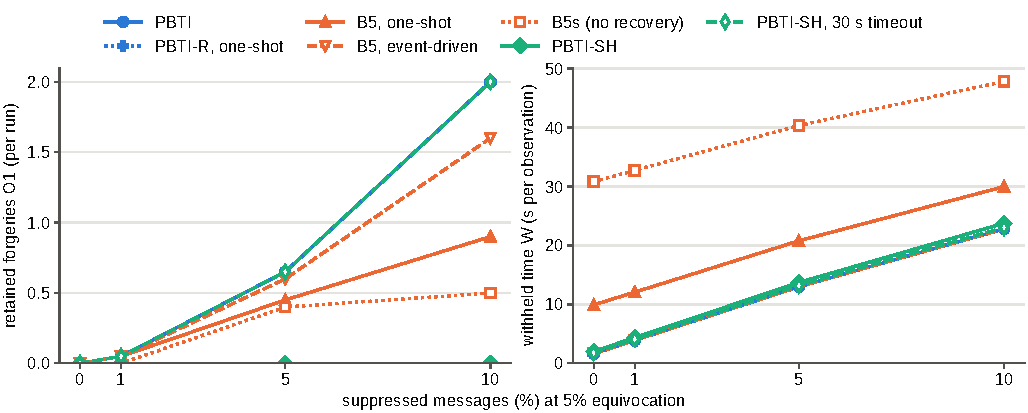
\includegraphics[width=\linewidth]{figures/fig_selective_grid.pdf}
\caption{Selective-hold grid at 5\% equivocation: retained forgeries O1 (left) and withheld time $W$ (right) versus the rate of suppressed messages (means of 20 paired seeds, seeds 21--40; 120~s production). One-shot: one-shot review rule with $R=60$~s and $C=10$~s (PBTI-R\textsubscript{60/10} and \Bhist); event-driven: \Bev. In the left panel \sys, PBTI-R\textsubscript{60/10} and PBTI-SH-T30 coincide. Colour marks the pipeline family, line style and marker the variant. All points: Table~\ref{tab:S-a3}.\label{fig:S-a3}}
\end{figure}

\noindent\textbf{Selective-hold factorial cells (amendment-informed).} Added after the freeze and before any confirmatory selective-hold run, because the pilot (seed 101) showed retained forgeries at only one of the \WAthreePoints\ points of the registered grid; with 20 seeds, the grid later showed small numbers at ten points (Table~\ref{tab:S-a3}). The amendment added the eight factorial cells with equivocation high (10\%), four of them with suppressed runs high (FG), on fresh seeds 21--40. \WAthreeFRuns\ runs, \WAthreeFErrors\ errors; the tracer matched in \WAthreeFTracerMatch\ runs and \WAthreeFAuditsPass\ of \WAthreeFAudits\ audited runs passed. Gates: G3F \WAthreeFGThree, G4F \WAthreeFGFour.
\begin{table}[!htbp]
\caption{Selective holds in the factorial cells (means over seeds 21--40; 120~s production, about 2{,}880 legitimate observations per run). FG: equivocation and suppressed runs both high.\label{tab:S-a3f}}
\footnotesize\centering
% AUTO-GENERATED by analysis/analyze_v4.py; labels neutralized by tools/v7/neutralize_tables.py
\begin{tabular}{@{}llrrrrr@{}}\toprule
Cell (high factors) & Arm & O1 & O2 & NLX (rec-s) & $W$ (s) & AV5 \\ \midrule
run2 & PBTI & 0.00 & 251.8 & 0 & 21.69 & 0.919 \\
(duplicates, clock error, & PBTI-SH & 0.00 & 286.4 & 0 & 24.69 & 0.904 \\
equivocation) & PBTI-SH-T30 & 0.00 & 251.8 & 0 & 22.17 & 0.904 \\
 & B5\textsubscript{60/10} & 0.00 & 256.3 & 0 & 29.78 & 0.793 \\
 & B5\textsubscript{ev} & 0.00 & 255.3 & 0 & 22.00 & 0.917 \\
 & B5S & 0.00 & 598.2 & 0 & 49.46 & 0.793 \\
 & PBTI-R\textsubscript{60/10} & 0.00 & 251.8 & 0 & 21.69 & 0.919 \\
\addlinespace[2pt]
run3$^{FG}$ & PBTI & 1.40 & 243.0 & 325 & 20.46 & 0.921 \\
(loss, duplicates, equivocation, & PBTI-SH & 0.00 & 256.1 & 0 & 21.60 & 0.910 \\
suppressed runs) & PBTI-SH-T30 & 1.40 & 243.0 & 281 & 20.73 & 0.910 \\
 & B5\textsubscript{60/10} & 0.40 & 246.0 & 62 & 28.72 & 0.791 \\
 & B5\textsubscript{ev} & 1.15 & 244.4 & 267 & 20.58 & 0.920 \\
 & B5S & 0.00 & 602.5 & 0 & 49.51 & 0.791 \\
 & PBTI-R\textsubscript{60/10} & 1.40 & 243.0 & 325 & 20.46 & 0.921 \\
\addlinespace[2pt]
run4$^{FG}$ & PBTI & 2.50 & 478.7 & 613 & 40.54 & 0.841 \\
(reordering, clock error, & PBTI-SH & 0.00 & 516.2 & 6 & 43.74 & 0.824 \\
equivocation, suppressed runs) & PBTI-SH-T30 & 2.50 & 478.7 & 536 & 41.04 & 0.824 \\
 & B5\textsubscript{60/10} & 0.85 & 484.1 & 185 & 47.86 & 0.727 \\
 & B5\textsubscript{ev} & 1.50 & 482.3 & 383 & 40.85 & 0.838 \\
 & B5S & 0.35 & 789.9 & 99 & 65.46 & 0.727 \\
 & PBTI-R\textsubscript{60/10} & 2.50 & 478.7 & 613 & 40.54 & 0.841 \\
\addlinespace[2pt]
run5 & PBTI & 0.00 & 43.0 & 0 & 3.97 & 0.991 \\
(loss, reordering, equivocation) & PBTI-SH & 0.00 & 47.0 & 0 & 4.37 & 0.982 \\
 & PBTI-SH-T30 & 0.00 & 43.0 & 0 & 4.16 & 0.982 \\
 & B5\textsubscript{60/10} & 0.00 & 43.4 & 0 & 12.59 & 0.852 \\
 & B5\textsubscript{ev} & 0.00 & 43.0 & 0 & 3.98 & 0.991 \\
 & B5S & 0.00 & 424.6 & 0 & 34.78 & 0.852 \\
 & PBTI-R\textsubscript{60/10} & 0.00 & 43.0 & 0 & 3.97 & 0.991 \\
\addlinespace[2pt]
run8$^{FG}$ & PBTI & 1.65 & 270.6 & 405 & 22.69 & 0.912 \\
(long delay, equivocation, & PBTI-SH & 0.00 & 282.7 & 2 & 23.76 & 0.902 \\
suppressed runs) & PBTI-SH-T30 & 1.65 & 270.6 & 354 & 22.95 & 0.902 \\
 & B5\textsubscript{60/10} & 0.50 & 273.9 & 96 & 30.99 & 0.785 \\
 & B5\textsubscript{ev} & 0.80 & 272.5 & 199 & 22.86 & 0.911 \\
 & B5S & 0.15 & 625.8 & 43 & 51.26 & 0.785 \\
 & PBTI-R\textsubscript{60/10} & 1.65 & 270.6 & 405 & 22.69 & 0.912 \\
\addlinespace[2pt]
run9 & PBTI & 0.00 & 241.0 & 0 & 21.42 & 0.913 \\
(loss, long delay, clock error, & PBTI-SH & 0.00 & 272.9 & 0 & 24.25 & 0.895 \\
equivocation) & PBTI-SH-T30 & 0.00 & 241.0 & 0 & 21.92 & 0.895 \\
 & B5\textsubscript{60/10} & 0.00 & 245.5 & 0 & 29.67 & 0.787 \\
 & B5\textsubscript{ev} & 0.00 & 243.6 & 0 & 21.66 & 0.911 \\
 & B5S & 0.00 & 592.9 & 0 & 49.61 & 0.787 \\
 & PBTI-R\textsubscript{60/10} & 0.00 & 241.0 & 0 & 21.42 & 0.913 \\
\addlinespace[2pt]
run14 & PBTI & 0.00 & 45.0 & 0 & 4.11 & 0.991 \\
(duplicates, reordering, & PBTI-SH & 0.00 & 49.0 & 0 & 4.51 & 0.982 \\
long delay, equivocation) & PBTI-SH-T30 & 0.00 & 45.0 & 0 & 4.31 & 0.982 \\
 & B5\textsubscript{60/10} & 0.00 & 45.4 & 0 & 12.97 & 0.853 \\
 & B5\textsubscript{ev} & 0.00 & 45.0 & 0 & 4.13 & 0.990 \\
 & B5S & 0.00 & 431.3 & 0 & 35.23 & 0.853 \\
 & PBTI-R\textsubscript{60/10} & 0.00 & 45.0 & 0 & 4.11 & 0.991 \\
\addlinespace[2pt]
run15$^{FG}$ & PBTI & 0.85 & 403.7 & 195 & 35.08 & 0.853 \\
(loss, duplicates, reordering, & PBTI-SH & 0.00 & 444.4 & 0 & 38.63 & 0.832 \\
long delay, clock error, & PBTI-SH-T30 & 0.85 & 403.7 & 167 & 35.67 & 0.832 \\
equivocation, suppressed runs) & B5\textsubscript{60/10} & 0.25 & 414.1 & 42 & 43.32 & 0.735 \\
 & B5\textsubscript{ev} & 0.50 & 410.1 & 117 & 35.62 & 0.850 \\
 & B5S & 0.00 & 737.5 & 0 & 61.83 & 0.735 \\
 & PBTI-R\textsubscript{60/10} & 0.85 & 403.7 & 195 & 35.08 & 0.853 \\
\addlinespace[2pt]
\bottomrule\end{tabular}

\end{table}

\begin{figure}[!htbp]
\centering
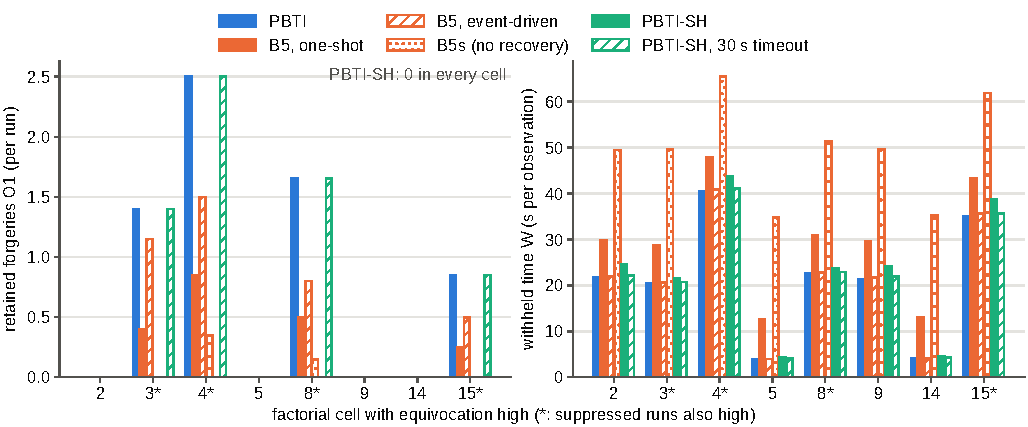
\includegraphics[width=\linewidth]{figures/fig_selective_cells.pdf}
\caption{Selective holds in the eight factorial cells with equivocation high (amendment-informed; means of 20 paired seeds, 120~s production, about 2880 legitimate observations per run): retained forgeries O1 (left) and withheld time $W$ (right). $^*$: suppressed runs also high. Colour marks the pipeline family (\sys\ blue, B5 orange, PBTI-SH aqua) and hatching the variant (one-shot: \Bhist; event-driven: \Bev); PBTI-R is identical to \sys\ in every cell and not shown. Values: Table~\ref{tab:S-a3f}.\label{fig:S-factorial}}
\end{figure}

\noindent All confirmatory comparisons, with mean differences, 95\% and 90\% bootstrap intervals, raw and Holm-adjusted $p$ and classes, are in Data~S1; the comparisons on which gates G3, G4, G3F and G4F depend follow. The class ``eq'' of the grid row with 5\% equivocation and 5\% suppressed messages (O1, versus \sys) is resampling-dependent: its 90\% interval touches $-1$, the margin, and the comparison of the same data with PBTI-R\textsubscript{60/10} is classed inconclusive in Data~S1; no gate depends on it. ``dw'' (different within the margin) means significant with a 95\% interval overlapping the margin, so the point estimate may exceed the margin.
\begingroup\footnotesize
% class wording adjusted by tools/manuscript/relabel_classes.py
% AUTO-GENERATED by analysis/analyze_v4.py; labels neutralized by tools/v7/neutralize_tables.py
\setlength{\tabcolsep}{2.6pt}
\begin{longtable}{@{}lllrrrllrl@{}}
\caption{Comparisons that decide the selective-hold gates: PBTI-SH versus the reference at the joint-grid points at which PBTI retained forgeries (G3: O1 or NLX better beyond the margin at half of these points; G4: G3 and $W$ not worse than B5\textsubscript{60/10} there) and in the factorial cells with equivocation and suppressed runs high (amendment 1; G3F: O1 or NLX better beyond the margin in at least two of the four cells; G4F: G3F and $W$ not worse than B5\textsubscript{60/10}). Means over seeds 21--40; $\bar d$ = PBTI-SH $-$ reference; Holm within campaign and outcome. Classes: id, identical in every seed; eq, equivalent within the margin (90\% CI inside $\pm$margin); eq$^{s}$, equivalent and significant after Holm correction; \textbf{B}/\textbf{W}, better/worse beyond the margin (Holm-adjusted $p<0.05$ and 95\% CI beyond the margin); dw, significant, margin unresolved (Holm-adjusted $p<0.05$, 95\% CI crossing a margin boundary; historical label ``different within the margin''); inc, inconclusive. All comparisons: Data~S1.}\label{tab:S-gates}\\
\toprule
Campaign & Point or cell & Ref. & Out. & SH & Ref. & $\bar d$ & 95\% CI & $p_\mathrm{Holm}$ & Class \\ \midrule\endfirsthead
\toprule
Campaign & Point or cell & Ref. & Out. & SH & Ref. & $\bar d$ & 95\% CI & $p_\mathrm{Holm}$ & Class \\ \midrule\endhead
grid & eq 1\%, supp. 5\% & PBTI & O1 & 0.15 & 0.25 & $-$0.1 & [$-$0.25, 0] & 1.000 & eq \\
 &  & PBTI & NLX & 39 & 64 & $-$25.1 & [$-$62.7, 0] & 1.000 & eq \\
 &  & B5\textsubscript{60/10} & W & 12.22 & 15.39 & $-$3.17 & [$-$3.77, $-$2.54] & $<$0.001 & \textbf{B} \\
\addlinespace[2pt]
grid & eq 1\%, supp. 10\% & PBTI & O1 & 0.10 & 0.25 & $-$0.15 & [$-$0.3, 0] & 1.000 & eq \\
 &  & PBTI & NLX & 24 & 53 & $-$29 & [$-$59, 0] & 1.000 & eq \\
 &  & B5\textsubscript{60/10} & W & 22.33 & 25.26 & $-$2.93 & [$-$3.49, $-$2.38] & $<$0.001 & \textbf{B} \\
\addlinespace[2pt]
grid & eq 5\%, supp. 1\% & PBTI & O1 & 0.00 & 0.05 & $-$0.05 & [$-$0.15, 0] & 1.000 & eq \\
 &  & PBTI & NLX & 0 & 11 & $-$11 & [$-$33, 0] & 1.000 & eq \\
 &  & B5\textsubscript{60/10} & W & 4.35 & 12.07 & $-$7.72 & [$-$7.98, $-$7.46] & $<$0.001 & \textbf{B} \\
\addlinespace[2pt]
grid & eq 5\%, supp. 5\% & PBTI & O1 & 0.00 & 0.65 & $-$0.65 & [$-$1.05, $-$0.3] & 0.618 & eq \\
 &  & PBTI & NLX & 5 & 162 & $-$157 & [$-$250, $-$74.2] & 0.830 & inc \\
 &  & B5\textsubscript{60/10} & W & 13.71 & 20.77 & $-$7.06 & [$-$7.3, $-$6.82] & $<$0.001 & \textbf{B} \\
\addlinespace[2pt]
grid & eq 5\%, supp. 10\% & PBTI & O1 & 0.00 & 2.00 & $-$2 & [$-$2.5, $-$1.45] & 0.021 & \textbf{B} \\
 &  & PBTI & NLX & 19 & 487 & $-$468 & [$-$595, $-$349] & 0.024 & \textbf{B} \\
 &  & B5\textsubscript{60/10} & W & 23.75 & 29.96 & $-$6.22 & [$-$6.55, $-$5.89] & $<$0.001 & \textbf{B} \\
\addlinespace[2pt]
grid & eq 5\%, long supp. 1\% & PBTI & O1 & 0.00 & 0.20 & $-$0.2 & [$-$0.55, 0] & 1.000 & eq \\
 &  & PBTI & NLX & 0 & 46 & $-$45.5 & [$-$126, 0] & 1.000 & inc \\
 &  & B5\textsubscript{60/10} & W & 3.84 & 11.69 & $-$7.85 & [$-$8.11, $-$7.59] & $<$0.001 & \textbf{B} \\
\addlinespace[2pt]
grid & eq 5\%, long supp. 5\% & PBTI & O1 & 0.00 & 1.85 & $-$1.85 & [$-$2.65, $-$1.1] & 0.159 & inc \\
 &  & PBTI & NLX & 20 & 430 & $-$409 & [$-$586, $-$241] & 0.168 & inc \\
 &  & B5\textsubscript{60/10} & W & 13.45 & 20.41 & $-$6.95 & [$-$7.42, $-$6.46] & $<$0.001 & \textbf{B} \\
\addlinespace[2pt]
grid & eq 10\%, supp. 1\% & PBTI & O1 & 0.00 & 0.25 & $-$0.25 & [$-$0.5, $-$0.05] & 1.000 & eq \\
 &  & PBTI & NLX & 0 & 56 & $-$56.2 & [$-$113, $-$11.4] & 1.000 & inc \\
 &  & B5\textsubscript{60/10} & W & 6.15 & 14.13 & $-$7.98 & [$-$8.15, $-$7.79] & $<$0.001 & \textbf{B} \\
\addlinespace[2pt]
grid & eq 10\%, supp. 5\% & PBTI & O1 & 0.00 & 1.20 & $-$1.2 & [$-$1.6, $-$0.85] & 0.034 & dw \\
 &  & PBTI & NLX & 6 & 295 & $-$290 & [$-$378, $-$202] & 0.035 & \textbf{B} \\
 &  & B5\textsubscript{60/10} & W & 15.45 & 22.74 & $-$7.29 & [$-$7.51, $-$7.09] & $<$0.001 & \textbf{B} \\
\addlinespace[2pt]
grid & eq 10\%, supp. 10\% & PBTI & O1 & 0.00 & 2.95 & $-$2.95 & [$-$3.75, $-$2.2] & 0.015 & \textbf{B} \\
 &  & PBTI & NLX & 7 & 724 & $-$717 & [$-$908, $-$528] & $<$0.001 & \textbf{B} \\
 &  & B5\textsubscript{60/10} & W & 25.43 & 32.15 & $-$6.72 & [$-$6.99, $-$6.44] & $<$0.001 & \textbf{B} \\
\addlinespace[2pt]
cells & run3$^{FG}$ & PBTI & O1 & 0.00 & 1.40 & $-$1.4 & [$-$1.8, $-$0.95] & 0.016 & dw \\
 &  & PBTI & NLX & 0 & 325 & $-$325 & [$-$419, $-$230] & 0.009 & \textbf{B} \\
 &  & PBTI & W & 21.60 & 20.46 & 1.14 & [1.02, 1.27] & $<$0.001 & \textbf{W} \\
 &  & PBTI & O2 & 256.1 & 243.0 & 13.1 & [11.6, 14.7] & 0.003 & eq$^{s}$ \\
 &  & PBTI & AV5 & 0.910 & 0.921 & $-$0.011 & [$-$0.0119, $-$0.0102] & 0.004 & \textbf{W} \\
 &  & B5\textsubscript{60/10} & W & 21.60 & 28.72 & $-$7.12 & [$-$7.33, $-$6.92] & $<$0.001 & \textbf{B} \\
 &  & B5\textsubscript{60/10} & O2 & 256.1 & 246.0 & 10.1 & [9, 11.2] & 0.003 & eq$^{s}$ \\
\addlinespace[2pt]
cells & run4$^{FG}$ & PBTI & O1 & 0.00 & 2.50 & $-$2.5 & [$-$3.2, $-$1.9] & 0.006 & \textbf{B} \\
 &  & PBTI & NLX & 6 & 613 & $-$607 & [$-$781, $-$455] & $<$0.001 & \textbf{B} \\
 &  & PBTI & W & 43.74 & 40.54 & 3.2 & [3.09, 3.32] & $<$0.001 & \textbf{W} \\
 &  & PBTI & O2 & 516.2 & 478.7 & 37.5 & [36.1, 38.9] & 0.003 & \textbf{W} \\
 &  & PBTI & AV5 & 0.824 & 0.841 & $-$0.0161 & [$-$0.0169, $-$0.0152] & 0.004 & \textbf{W} \\
 &  & B5\textsubscript{60/10} & W & 43.74 & 47.86 & $-$4.12 & [$-$4.28, $-$3.95] & $<$0.001 & \textbf{B} \\
 &  & B5\textsubscript{60/10} & O2 & 516.2 & 484.1 & 32 & [31.1, 33.1] & 0.003 & \textbf{W} \\
\addlinespace[2pt]
cells & run8$^{FG}$ & PBTI & O1 & 0.00 & 1.65 & $-$1.65 & [$-$2.5, $-$0.95] & 0.021 & dw \\
 &  & PBTI & NLX & 2 & 405 & $-$403 & [$-$589, $-$242] & 0.009 & \textbf{B} \\
 &  & PBTI & W & 23.76 & 22.69 & 1.07 & [0.944, 1.2] & $<$0.001 & \textbf{W} \\
 &  & PBTI & O2 & 282.7 & 270.6 & 12.2 & [10.6, 13.7] & 0.003 & eq$^{s}$ \\
 &  & PBTI & AV5 & 0.902 & 0.912 & $-$0.0104 & [$-$0.0112, $-$0.00964] & 0.004 & dw \\
 &  & B5\textsubscript{60/10} & W & 23.76 & 30.99 & $-$7.23 & [$-$7.47, $-$6.99] & $<$0.001 & \textbf{B} \\
 &  & B5\textsubscript{60/10} & O2 & 282.7 & 273.9 & 8.8 & [7.9, 9.75] & 0.003 & eq$^{s}$ \\
\addlinespace[2pt]
cells & run15$^{FG}$ & PBTI & O1 & 0.00 & 0.85 & $-$0.85 & [$-$1.3, $-$0.45] & 0.092 & inc \\
 &  & PBTI & NLX & 0 & 195 & $-$194 & [$-$300, $-$102] & 0.024 & \textbf{B} \\
 &  & PBTI & W & 38.63 & 35.08 & 3.55 & [3.35, 3.74] & $<$0.001 & \textbf{W} \\
 &  & PBTI & O2 & 444.4 & 403.7 & 40.7 & [38.2, 43.1] & 0.003 & \textbf{W} \\
 &  & PBTI & AV5 & 0.832 & 0.853 & $-$0.0211 & [$-$0.0222, $-$0.02] & 0.004 & \textbf{W} \\
 &  & B5\textsubscript{60/10} & W & 38.63 & 43.32 & $-$4.69 & [$-$5.03, $-$4.33] & $<$0.001 & \textbf{B} \\
 &  & B5\textsubscript{60/10} & O2 & 444.4 & 414.1 & 30.4 & [28.2, 32.4] & 0.003 & dw \\
\bottomrule\end{longtable}

\endgroup

\begin{table}[!htbp]
\caption{Selective-hold controls: \sys\ (re-executed main-evaluation rows) and PBTI-SH on the 16 workloads, and PBTI-SH-T30 on four of them (means over seeds 1--20; descriptive).\label{tab:S-a3-scen}}
\footnotesize\centering
% AUTO-GENERATED by analysis/analyze_v4.py; labels neutralized by tools/v7/neutralize_tables.py
\begin{tabular}{@{}lrrrrrrrrrr@{}}\toprule
 & \multicolumn{2}{c}{O1} & \multicolumn{2}{c}{O2} & \multicolumn{2}{c}{NLX (rec-s)} & \multicolumn{2}{c}{$W$ (s)} & \multicolumn{2}{c}{AV5} \\ \cmidrule(lr){2-3}\cmidrule(lr){4-5}\cmidrule(lr){6-7}\cmidrule(lr){8-9}\cmidrule(lr){10-11}
Scenario & PBTI & SH & PBTI & SH & PBTI & SH & PBTI & SH & PBTI & SH \\ \midrule
E1 & 0.0 & 0.0 & 0.0 & 0.0 & 0 & 0 & 0.03 & 0.03 & 1.000 & 1.000 \\
E2 & 0.0 & 0.0 & 354.9 & 354.9 & 0 & 0 & 16.28 & 16.28 & 0.951 & 0.951 \\
E3 & 0.0 & 0.0 & 427.7 & 427.7 & 0 & 0 & 19.55 & 19.55 & 0.941 & 0.941 \\
E4 & 0.0 & 0.0 & 0.0 & 0.0 & 0 & 0 & 0.03 & 0.03 & 1.000 & 1.000 \\
E5 & 150.0 & 150.0 & 222.6 & 225.6 & 38{,}266 & 38{,}242 & 8.64 & 8.81 & 0.972 & 0.969 \\
E6 & 0.0 & 0.0 & 0.0 & 0.0 & 0 & 0 & 0.03 & 0.03 & 1.000 & 1.000 \\
E7 & 0.0 & 0.0 & 0.0 & 0.0 & 0 & 0 & 0.07 & 0.07 & 1.000 & 1.000 \\
E8 & 0.0 & 0.0 & 12.0 & 14.0 & 0 & 0 & 0.56 & 0.67 & 0.999 & 0.999 \\
E9 & 0.0 & 0.0 & 0.0 & 0.0 & 0 & 0 & 0.47 & 0.47 & 1.000 & 1.000 \\
E10 & 0.0 & 0.0 & 0.0 & 0.0 & 0 & 0 & 0.07 & 0.07 & 1.000 & 1.000 \\
E11/12 & 0.0 & 0.0 & 0.0 & 0.0 & 0 & 0 & 6.76 & 6.76 & 0.889 & 0.889 \\
E11b & 0.0 & 0.0 & 193.3 & 193.3 & 0 & 0 & 17.54 & 17.54 & 0.867 & 0.867 \\
E13 & 0.0 & 0.0 & 0.0 & 0.0 & 0 & 0 & 6.59 & 6.59 & 0.894 & 0.894 \\
E14 & 0.0 & 0.0 & 270.1 & 270.1 & 8{,}042 & 8{,}042 & 11.41 & 11.41 & 0.974 & 0.974 \\
E15 & 15.8 & 15.8 & 89.5 & 89.5 & 5{,}145 & 5{,}145 & 4.11 & 4.11 & 0.988 & 0.988 \\
Mixed & 5.2 & 5.0 & 335.0 & 361.6 & 3{,}462 & 3{,}284 & 22.95 & 24.17 & 0.847 & 0.841 \\
\midrule
\multicolumn{11}{@{}l}{SH = PBTI-SH-T30 (30~s timeout):} \\
E5 & 150.0 & 150.0 & 222.6 & 222.6 & 38{,}266 & 38{,}242 & 8.64 & 8.75 & 0.972 & 0.969 \\
E8 & 0.0 & 0.0 & 12.0 & 12.0 & 0 & 0 & 0.56 & 0.63 & 0.999 & 0.999 \\
E14 & 0.0 & 0.0 & 270.1 & 270.1 & 8{,}042 & 8{,}042 & 11.41 & 11.41 & 0.974 & 0.974 \\
Mixed & 5.2 & 5.2 & 335.0 & 335.0 & 3{,}462 & 3{,}341 & 22.95 & 23.18 & 0.847 & 0.841 \\
\bottomrule\end{tabular}

\end{table}

\begin{table}[!htbp]
\caption{Lifecycle analysis of reviewed release under revoked credentials (deterministic; repository \texttt{scripts/\allowbreak{}a5\_\allowbreak{}lifecycle\_\allowbreak{}matrix.py}): device and relay keys compromised at $t_c=10$~s, revocation observed at 20~s with $t_\mathrm{comp}=10$~s, reviewer decisions at 30~s (in the superseded-snapshot case a decision at \YEnineRefusedAt~s bound to a superseded snapshot is refused first), ticks to 60~s. Release-evidence policies of the REVOKED\_BUFFERED waiver: none; discretionary (the observation's own time stamp precedes $t_\mathrm{comp}$; used in all scenario campaigns); witness (a token from a time-stamping witness for the exact statement digest, witness time plus clock uncertainty (1~s) before $t_\mathrm{low}$). \sys\ and B5 gave \WAfivePBTIBfiveSame\ results. The interval row sets $t_\mathrm{low}=t_c-$ width/2. The witness's key and clock are trusted by assumption.\label{tab:S-a5}}
\footnotesize\centering
% row label extended by tools/manuscript/relabel_rows.py
% AUTO-GENERATED by analysis/analyze_v4.py; labels neutralized by tools/v7/neutralize_tables.py
\begin{tabularx}{\linewidth}{@{}>{\raggedright\arraybackslash}p{4.3cm}*{3}{>{\centering\arraybackslash}X}@{}}\toprule
Case (PBTI; B5 identical) & none & discretionary & witness \\ \midrule
Legitimate buffered record, witnessed before $t_c$ & withheld (rejected) & recovered & recovered \\
Backdated forgery, witness sees it after $t_c$ & excluded (rejected) & \textbf{forgery authoritative} & excluded (rejected) \\
Backdated forgery, never witnessed & excluded (rejected) & \textbf{forgery authoritative} & excluded (rejected) \\
Forgery contradicted by an admitted successor & excluded (rejected) & excluded (rejected) & excluded (rejected) \\
Legitimate record, witness outage & withheld (rejected) & recovered & withheld (rejected) \\
Decision on a superseded snapshot (refused at \YEnineRefusedAt~s; released by a fresh decision at \YEnineFreshAt~s) & recovered & recovered & recovered \\
Reviewer key revoked & withheld (quarantined) & withheld (quarantined) & withheld (quarantined) \\
STALE\_TS case, origin revoked before release & withheld (rejected) & withheld (rejected) & withheld (rejected) \\
Released, later revocation covers commit time & released, then tainted & released, then tainted & released, then tainted \\
Released under revoked key, then earlier $t_{comp}$ revision & withheld (rejected) & released, then tainted; window corrected & released, then tainted; window corrected \\
\midrule
Interval width $t_{high}-t_{low}$ (witness policy) & \multicolumn{3}{l}{0\,s: recovered; 5\,s: recovered; 30\,s: withheld; 120\,s: withheld} \\
\bottomrule\end{tabularx}

\end{table}

\section{Revocation, Sensitivity Analyses, Replay, Ablation and Insider Tampering}\label{sec:S-sens}
\noindent\textbf{Revocation.} With immediate status refresh ($\Delta=0$), \sys\ tainted \RRevPBTItaint\ commits per run in E14; with a 30~s refresh, \RRevPBTIThreeZerospost\ post-revocation injections per run passed before the refresh and were tainted once the revocation was observed.
\begin{table}[!htbp]
\caption{Revocation (E14): post-revocation admissions of attacks with revoked keys, and non-legitimate observations remaining authoritative at the end of the run, by status refresh interval $\Delta$ (means over \RRevSeeds\ seeds).\label{tab:S-revocation}}
\centering
\footnotesize
\begin{tabular}{rrrrrrrrr}
\toprule
& \multicolumn{2}{c}{B1} & \multicolumn{2}{c}{B2} & \multicolumn{2}{c}{B3} & \multicolumn{2}{c}{PBTI}\\
\cmidrule(lr){2-3}\cmidrule(lr){4-5}\cmidrule(lr){6-7}\cmidrule(lr){8-9}
Status refresh $\Delta$ & post-rev. & non-legit. & post-rev. & non-legit. & post-rev. & non-legit. & post-rev. & non-legit.\\
\midrule
0 s & 40 & 239.9 & 0 & 199.9 & 0 & 199.9 & 0 & 0\\
1 s & 40 & 239.9 & 0 & 199.9 & 0 & 199.9 & 0 & 0\\
5 s & 40 & 239.9 & 0 & 199.9 & 0 & 199.9 & 0 & 0\\
30 s & 40 & 239.9 & 3 & 202.9 & 3 & 202.9 & 3 & 0\\
\bottomrule
\end{tabular}
\end{table}

\begin{figure}[!htbp]
\centering
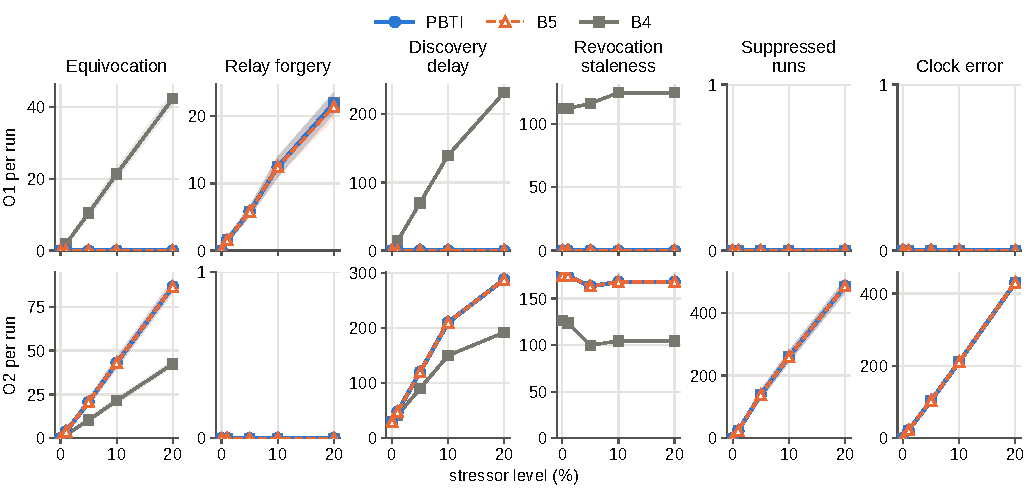
\includegraphics[width=\linewidth]{figures/fig_sweep.pdf}
\caption{Stressor sweep: non-legitimate observations authoritative at the end of the run (O1, top) and legitimate observations missing (O2, bottom) per run versus stressor level for \sys, B5 and B4 (means of 20 paired seeds, shaded 95\% bootstrap intervals; 120~s production phase, 2880 legitimate observations per run; exploratory). Where B5 coincides with \sys, its dashed line overlays \sys's. For the five remaining factors (loss, duplicates, reordering, long delay and outage bursts, levels 0--20\%), both outcomes were zero at every level for all three pipelines (stored summary in Data~S1). Definitions of all factors and levels: repository \texttt{docs/\allowbreak{}V3\_\allowbreak{}SWEEP\_\allowbreak{}DESIGN.md}.\label{fig:S-sweep}}
\end{figure}

\begin{table}[!htbp]
\caption{Fractional factorial $2^{7-3}_\mathrm{IV}$ at 0 and 10\%: estimated effects on O1 and O2 per run (mean over 20 seeds of the per-seed effect; $^{*}$: 95\% $t$ interval excludes 0; exploratory). A loss, B duplicates, C reordering, D long delay, E clock error ($=ABC$), F equivocation ($=BCD$), G suppressed runs ($=ACD$); main effects are aliased with three-factor interactions, two-factor interactions in the chains shown.\label{tab:S-factorial}}
\footnotesize\centering
\begin{tabular}{lrrrrrr}
\toprule
& \multicolumn{2}{c}{\textbf{PBTI}} & \multicolumn{2}{c}{\textbf{B4}} & \multicolumn{2}{c}{\textbf{B5}}\\
\cmidrule(lr){2-3}\cmidrule(lr){4-5}\cmidrule(lr){6-7}
\textbf{Effect} & O1 & O2 & O1 & O2 & O1 & O2\\
\midrule
A (loss) & -0.0 & -10.0$^{*}$ & 0.1 & -9.9$^{*}$ & 0.1 & -9.4$^{*}$\\
B (dup) & -0.0 & -10.7$^{*}$ & -0.0 & -10.7$^{*}$ & 0.1 & -10.1$^{*}$\\
C (reorder) & 0 & -1.6$^{*}$ & -0.3 & -2.7$^{*}$ & -0.0 & -1.4\\
D (delay) & -0.1 & -15.2$^{*}$ & 0.5 & -15.8$^{*}$ & -0.0 & -14.6$^{*}$\\
E (clock) & 0 & 193.6$^{*}$ & -0.9$^{*}$ & 194.5$^{*}$ & -0.0 & 195.9$^{*}$\\
F (equivocation) & 1.1$^{*}$ & 42.1$^{*}$ & 21.6$^{*}$ & 20.5$^{*}$ & 0.4$^{*}$ & 46.2$^{*}$\\
G (missing) & 1.1$^{*}$ & 210.6$^{*}$ & 0.9$^{*}$ & 211.4$^{*}$ & 0.4$^{*}$ & 212.1$^{*}$\\
AB = CE = FG & 1.1$^{*}$ & -1.3$^{*}$ & 0.9$^{*}$ & -0.5 & 0.4$^{*}$ & 0.1\\
AC = BE = DG & -0.1 & -9.4$^{*}$ & 0.3 & -9.2$^{*}$ & -0.0 & -9.0$^{*}$\\
AD = EF = CG & 0 & -3.9$^{*}$ & -0.9$^{*}$ & -3.0$^{*}$ & -0.0 & -1.6$^{*}$\\
AE = BC = DF & -0.1 & 2.1$^{*}$ & 0.5 & 1.5$^{*}$ & -0.0 & 2.7$^{*}$\\
AF = DE = BG & -0.0 & -17.5$^{*}$ & 0.1 & -17.4$^{*}$ & 0.1 & -16.9$^{*}$\\
AG = CD = BF & -0.0 & -9.8$^{*}$ & -0.0 & -9.9$^{*}$ & 0.1 & -9.2$^{*}$\\
BD = CF = EG & 0 & -7.4$^{*}$ & -0.3 & -8.6$^{*}$ & -0.0 & -7.2$^{*}$\\
\bottomrule
\end{tabular}
\end{table}

\begin{table}[!htbp]
\caption{Replay of SKAB telemetry with injected, labelled stressors (means over 20 seeds; about 14{,}400 legitimate observations per run; exploratory). Avail.: share of reachable legitimate observations authoritative at the end, in rows that SKAB labels normal or anomalous (process anomalies, not attacks). Unstressed controls: \VRpCleanRuns\ runs with \VRpCleanMissingTotal\ missing and \VRpCleanNonlegitTotal\ non-legitimate observations in total. Attributed re-runs traced \VRpResPBTIgw\ of the \VRpResPBTItotal\ observations retained by \sys\ and all \VRpResBFivetotal\ retained by B5 to a compromised, never-revoked gateway forging its legacy device's data, and \VRpResBFourimp\ of B4's \VRpResBFourtotal\ to impersonation that B4 cannot taint.\label{tab:S-skab}}
\footnotesize\centering
\begin{tabular}{rlrrrrrrrr}
\toprule
\textbf{Speed} & \textbf{Pipeline} & \textbf{Reach.} & \textbf{Non-legit.} & \textbf{Missing} & \textbf{Quar.} & \textbf{Held} & \textbf{Released (p50 s)} & \textbf{Avail.\ normal \%} & \textbf{Avail.\ anomaly \%}\\
\midrule
1$\times$ & B4 & 14{,}400 & 192.1 & 190.2 & 0 & 0 & 0 & 98.5 & 98.8\\
1$\times$ & B5 & 14{,}400 & 11.3 & 303.2 & 52.6 & 2572.2 & 2370.8 (65.2) & 98.2 & 97.7\\
1$\times$ & PBTI & 14{,}400 & 11.3 & 303.1 & 0 & 0 & 0 & 98.2 & 97.7\\
5$\times$ & B4 & 14{,}400 & 175.3 & 306.3 & 0 & 0 & 0 & 97.8 & 97.9\\
5$\times$ & B5 & 14{,}400 & 10.4 & 418.9 & 51.8 & 2567.2 & 2359.9 (65.3) & 97.5 & 96.8\\
5$\times$ & PBTI & 14{,}400 & 10.9 & 418.9 & 0 & 0 & 0 & 97.5 & 96.8\\
10$\times$ & B4 & 14{,}400 & 171.2 & 448.8 & 0 & 0 & 0 & 96.9 & 96.8\\
10$\times$ & B5 & 14{,}400 & 10.2 & 562.1 & 51.6 & 2571.8 & 2358.6 (65.9) & 96.6 & 95.8\\
10$\times$ & PBTI & 14{,}400 & 10.4 & 562.1 & 0 & 0 & 0 & 96.6 & 95.8\\
\bottomrule
\end{tabular}
\end{table}

\begin{table}[!htbp]
\caption{Ablation study on the mixed workload (means over \RAblSeeds\ seeds; baseline rows give B1--B4 on the same workload for reference; $^{*}$: Holm-corrected Wilcoxon $p<0.05$ versus full \sys). Non-legit.: non-legitimate authoritative observations; Quar.: missing observations held in the quarantine archive; Ab1--Ab12: ablated variants.\label{tab:S-ablation}}
\centering
\footnotesize
\begin{tabular}{lrrrrrr}
\toprule
\textbf{Configuration} & \textbf{Non-legit.} & \textbf{Missing} & \textbf{Quar.} & \textbf{Dup.} & \textbf{CV wrong \%} & \textbf{$\mu$s/msg}\\
\midrule
B1 (baseline) & 485.5 & 282.6 & 0 & 0 & 28.1 & 51\\
B2 (baseline) & 380.3 & 340.9 & 0 & 0 & 22.8 & 53\\
B3 (baseline) & 215.1 & 272.6 & 0 & 0 & 6.8 & 239\\
B4 (baseline) & 147.7 & 327.6 & 0 & 0 & 3.5 & 266\\
\midrule
PBTI (full) & 5.2 & 335 & 60.1 & 0 & 0.8 & 494\\
Ab1 no relay signature & 5.9$^{*}$ & 362.4$^{*}$ & 60.6 & 0 & 3.2$^{*}$ & 323$^{*}$\\
Ab2 static policy & 30.4$^{*}$ & 482.3$^{*}$ & 60.1 & 0 & 3.6$^{*}$ & 478\\
Ab3 no origin signature & 30.1$^{*}$ & 335 & 60.1 & 0 & 21.0$^{*}$ & 342$^{*}$\\
Ab4 no prev link & 14.3$^{*}$ & 332.8$^{*}$ & 60.1 & 0 & 0.8 & 484\\
Ab5 edge-assigned identity & 72$^{*}$ & 273$^{*}$ & 60.0 & 48.1$^{*}$ & 1.0$^{*}$ & 495\\
Ab6 no conflict detection & 40.7$^{*}$ & 300.2$^{*}$ & 60.1 & 0 & 1.0$^{*}$ & 478\\
Ab7 no horizon/epoch checks & 35.1$^{*}$ & 274.9$^{*}$ & 0$^{*}$ & 0 & 4.6$^{*}$ & 489\\
Ab8 arrival-order state & 5.2 & 335 & 60.1 & 0 & 7.4$^{*}$ & 481\\
Ab9 no evidence commitment & 5.2 & 335 & 0$^{*}$ & 0 & 0.8 & 424$^{*}$\\
Ab10 no quarantine & 5.2 & 335 & 0$^{*}$ & 0 & 0.8 & 477\\
Ab11 no revocation/taint & 45.5$^{*}$ & 329.9$^{*}$ & 60.1 & 0 & 0.8$^{*}$ & 475\\
Ab12 volatile edge buffer & 5.0 & 517.5$^{*}$ & 60.6 & 0 & 0.8 & 498\\
\bottomrule
\end{tabular}
\end{table}

\begin{table}[!htbp]
\caption{Detection of insider tampering by the offline auditor (runs with detection / runs; 50 objects altered per run, or one checkpoint deleted for T4). Re-run with the final auditor (\VTamperRerunRuns\ runs): the same detection outcome in \VTamperRerunSameDetection, \sys\ detected \VTamperRerunPBTIDetected\ of \VTamperRerunPBTIRuns, and the same check families fired (in T2 decision replay additionally reports disposition mismatches).\label{tab:S-audit}}
\centering
\footnotesize
\begin{tabular}{lrrl}
\toprule
\textbf{Insider action} & \textbf{B3 detected} & \textbf{PBTI detected} & \textbf{PBTI checks that fired}\\
\midrule
T1 raw object modified & 5/5 & 5/5 & A-DET, A-LIN, A-RAW\\
T2 raw object deleted & 5/5 & 5/5 & A-DET, A-LIN, A-RAW\\
T3 evidence record modified & 5/5 & 5/5 & A-DET, A-EVID, A-REG\\
T4 checkpoint deleted & 0/5 & 5/5 & A-EVID\\
T5 log rewritten + re-signed (key holder) & 0/5 & 5/5 & A-DET, A-EVID, A-REG\\
T6 derived record modified & 0/5 & 5/5 & A-LIN\\
T7 registry state modified & 0/5 & 5/5 & A-DET, A-LIN\\
\bottomrule
\end{tabular}
\end{table}

\noindent\textbf{Review-workflow tests.} The workflow is covered by unit tests: release of a stale quarantined observation by an authorized reviewer with a signed evidence record; refusal of an unauthorized reviewer and of a decision with an invalid signature; idempotent duplicate decision, unknown case and revoked reviewer; stale review and conflicting evidence (release fails, slot contested); rejection of an uncorroborated forgery; re-taint of a released observation after a later revocation with recomputation of the current value; recovery after a long gap with a five-second gap horizon; B5 feed hold and release; B5s frozen feed with a new epoch admitted; state determinism over 120 delivery permutations; 15 handcrafted traces of the time-dependent outcomes; the deferring and event-driven review rules and the selective-hold gate; and the witness tokens, lifecycle cases and the complete revocation--quarantine--review--release--taint--correction sequence.

\section{Performance and Deployment}\label{sec:S-perf}
\noindent Figure~\ref{fig:S-perf} shows the in-process batching and worker study, the per-stage cost of \sys\ and the MQTT/TLS latency reported in the article's Section~\Mref{sec:res-perf}.
\begin{figure}[!htbp]
\centering
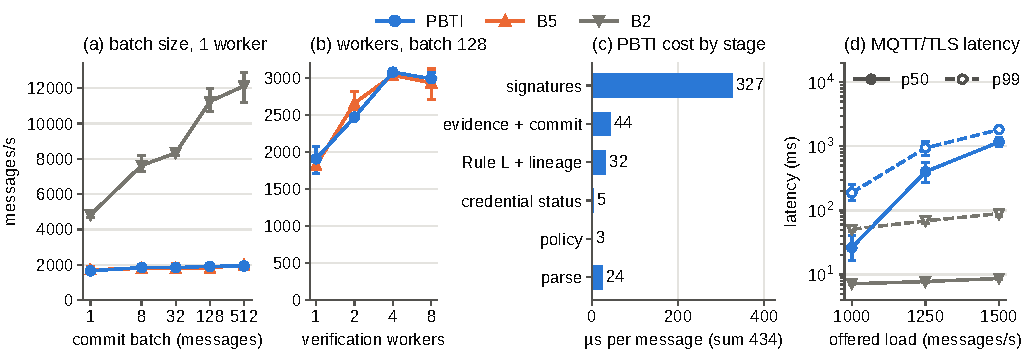
\includegraphics[width=\linewidth]{figures/fig_performance_costs.pdf}
\caption{(\textbf{a}) In-process throughput versus group-commit batch size (one worker; mean and 95\% CI, \VBtReps\ repetitions). (\textbf{b}) \sys\ and B5 versus signature-verification workers on two vCPUs (batch 128). (\textbf{c}) \sys\ cost by stage (in-process benchmark; Rule L and lineage without the nested commit time, so that the stages add up to the per-message total). (\textbf{d}) MQTT/TLS latency on one host with all roles co-located, p50 (solid) and p99 (dashed), mean and 95\% CI of \VEeReps\ repetitions. Colours as in the article's Figure~\Mref{fig:delay} (\sys\ blue, B5 orange); B2 grey.\label{fig:S-perf}}
\end{figure}

\noindent\textbf{Containers and hardware protocols.} A hardened container image (base pinned by digest, pinned Debian packages, hash-locked Python dependencies, non-root user, health check) built and passed the unit tests, a smoke run and an MQTT/TLS run, also with a read-only root file system and all capabilities dropped. The repository specifies a three-host MQTT/TLS deployment (edge publisher, broker, verifier; clock synchronization, RTT, bandwidth, 30 repetitions per cell) and a constrained-device signing benchmark (Raspberry-Pi-class; thermal state, power mode, energy). No separate hosts or constrained devices were available, so neither experiment was performed; no result in the article comes from them, and containers on one host are not reported as a multi-host deployment.

{\raggedright\noindent\textbf{Reproduction.} \texttt{python3 -m pytest -q tests/\allowbreak{}}; the campaign commands of Table~\ref{tab:S-stages}; \texttt{python3 scripts/\allowbreak{}compare\_\allowbreak{}a0.py results/\allowbreak{}v4/\allowbreak{}raw/\allowbreak{}A0\_\allowbreak{}core.jsonl}; \texttt{python3 scripts/\allowbreak{}a5\_\allowbreak{}lifecycle\_\allowbreak{}matrix.py}; \texttt{python3 formal/\allowbreak{}v4\_\allowbreak{}locality\_\allowbreak{}lifecycle\_\allowbreak{}check.py}; \texttt{python3 analysis/\allowbreak{}analyze\_\allowbreak{}v4.py}; then the paper build. On the two-vCPU reference host the confirmatory and re-execution campaigns took about six hours; the minimal reproduction kit (\texttt{tools/\allowbreak{}reexec/\allowbreak{}reproduce\_\allowbreak{}subset.sh}) took 81~minutes on two shared vCPUs in the second re-execution and reports every difference.\par}


\begin{table}[!htbp]
\caption{In-process verifier results with SQLite group commit (write-ahead logging, \texttt{synchronous=\allowbreak{}NORMAL}: a commit survives an application crash but can be rolled back by a power loss or operating-system crash; means over \RTpReps\ repetitions; one two-vCPU host). With \RTpReps\ repetitions per pipeline, normality cannot be established reliably (Shapiro--Wilk minimum $p=\RShapiroMinP$), so non-parametric tests were used.\label{tab:S-throughput}}
\footnotesize\centering
\begin{tabular}{lrrrrrrr}
\toprule
Pipeline & \makecell[r]{Throughput (msg/s)\\{[95\% CI]}} & \makecell[r]{CPU\\($\mu$s/msg)} & \makecell[r]{Service\\p50 ($\mu$s)} & \makecell[r]{Service\\p99 ($\mu$s)} & \makecell[r]{Wire\\(B/msg)} & \makecell[r]{Stored\\(B/msg)} & \makecell[r]{Edge CPU\\($\mu$s/msg)}\\
\midrule
B1 & 11358 [11079, 11580] & 73 & 33 & 139 & 219 & 674 & 38\\
B2 & 10707 [10410, 10946] & 78 & 38 & 158 & 220 & 674 & 36\\
B3 & 3329 [3298, 3362] & 281 & 222 & 581 & 292 & 1066 & 118\\
PBTI & 2067 [2039, 2093] & 466 & 402 & 1021 & 641 & 909 & 291\\
\bottomrule
\end{tabular}
\end{table}

\begin{table}[!htbp]
\caption{Verifier saturation throughput (messages/s) by number of devices (in-process, SQLite group commit as in Table~\ref{tab:S-throughput}; means of \RScaleReps\ repetitions).\label{tab:S-scaling}}
\footnotesize\centering
\begin{tabular}{lrrrr}
\toprule
Pipeline & 10 devices & 100 devices & 500 devices & 2000 devices\\
\midrule
B1 & 11583 & 10525 & 10924 & 10366\\
B2 & 10732 & 10012 & 10496 & 10043\\
B3 & 3360 & 3216 & 3142 & 3067\\
PBTI & 2054 & 2064 & 2018 & 1945\\
\bottomrule
\end{tabular}
\end{table}

\begin{table}[!htbp]
\caption{In-process batching and worker study (\VBtN\ messages per run, \VBtReps\ repetitions per cell, randomized order; 2 vCPUs). Latency: time from dispatch of a message's batch to its commit at saturation (the fill time of a batch at an open-loop arrival rate comes on top). Disposition sequences were \VBatchSemanticsIdentical\ across all cells of a pipeline.\label{tab:S-batching}}
\footnotesize\centering
\begin{tabular}{lrrrrrrrr}
\toprule
\textbf{Pipeline} & \textbf{Batch} & \textbf{Workers} & \textbf{msg/s [95\% CI]} & \textbf{p50 (ms)} & \textbf{p99 (ms)} & \textbf{CPU cores} & \textbf{CPU $\mu$s/msg} & \textbf{DB B/msg}\\
\midrule
B2 & 1 & 1 & 4818 [4682, 4997] & 0.1 & 1.0 & 0.64 & 133 & 673\\
B2 & 8 & 1 & 7627 [7259, 8192] & 0.5 & 13.8 & 0.70 & 92 & 673\\
B2 & 32 & 1 & 8328 [8176, 8591] & 2.3 & 19.9 & 0.75 & 90 & 673\\
B2 & 128 & 1 & 11250 [10677, 11988] & 7.5 & 48.1 & 0.83 & 74 & 673\\
B2 & 512 & 1 & 12124 [11188, 12869] & 32.8 & 86.7 & 0.90 & 75 & 673\\
B5 & 1 & 1 & 1720 [1584, 1888] & 0.5 & 1.3 & 0.93 & 542 & 911\\
B5 & 8 & 1 & 1786 [1679, 1851] & 3.7 & 17.3 & 0.94 & 526 & 911\\
B5 & 32 & 1 & 1808 [1555, 2087] & 15.5 & 41.7 & 0.95 & 536 & 911\\
B5 & 128 & 1 & 1820 [1715, 1952] & 65.0 & 122.2 & 0.97 & 533 & 911\\
B5 & 128 & 2 & 2659 [2568, 2814] & 91.8 & 141.5 & 1.61 & 606 & 911\\
B5 & 128 & 4 & 3037 [3017, 3050] & 160.5 & 229.8 & 1.79 & 591 & 911\\
B5 & 128 & 8 & 2935 [2710, 3122] & 325.3 & 555.9 & 1.77 & 606 & 911\\
B5 & 512 & 1 & 1988 [1839, 2069] & 237.2 & 374.0 & 0.98 & 494 & 911\\
PBTI & 1 & 1 & 1651 [1584, 1708] & 0.5 & 1.3 & 0.93 & 562 & 911\\
PBTI & 1 & 2 & 862 [850, 878] & 1.9 & 7.3 & 1.18 & 1366 & 911\\
PBTI & 1 & 4 & 1113 [1051, 1145] & 3.1 & 14.6 & 1.30 & 1166 & 911\\
PBTI & 1 & 8 & 1255 [1229, 1272] & 5.7 & 18.4 & 1.33 & 1{,}063 & 911\\
PBTI & 8 & 1 & 1841 [1762, 1911] & 3.5 & 16.6 & 0.95 & 514 & 911\\
PBTI & 8 & 2 & 1618 [1543, 1674] & 9.1 & 24.6 & 1.23 & 762 & 911\\
PBTI & 8 & 4 & 1842 [1702, 2070] & 16.2 & 40.3 & 1.42 & 774 & 911\\
PBTI & 8 & 8 & 2056 [1935, 2170] & 29.6 & 60.7 & 1.54 & 750 & 911\\
PBTI & 32 & 1 & 1836 [1713, 1919] & 14.9 & 37.3 & 0.95 & 521 & 911\\
PBTI & 32 & 2 & 2037 [1981, 2143] & 29.6 & 55.3 & 1.33 & 651 & 911\\
PBTI & 32 & 4 & 2428 [2280, 2547] & 50.0 & 97.7 & 1.59 & 654 & 911\\
PBTI & 32 & 8 & 2589 [2370, 2766] & 93.2 & 173.4 & 1.66 & 645 & 911\\
PBTI & 128 & 1 & 1908 [1713, 2077] & 60.4 & 140.7 & 0.96 & 508 & 911\\
PBTI & 128 & 2 & 2470 [2438, 2492] & 98.9 & 156.8 & 1.59 & 642 & 911\\
PBTI & 128 & 4 & 3078 [3039, 3133] & 157.5 & 236.2 & 1.79 & 580 & 911\\
PBTI & 128 & 8 & 2989 [2872, 3080] & 325.2 & 497.7 & 1.78 & 596 & 911\\
PBTI & 512 & 1 & 1924 [1891, 1948] & 259.3 & 364.8 & 0.97 & 504 & 911\\
PBTI & 512 & 2 & 2861 [2732, 2973] & 333.9 & 456.2 & 1.74 & 610 & 911\\
PBTI & 512 & 4 & 3184 [3121, 3283] & 594.7 & 879.0 & 1.81 & 568 & 911\\
PBTI & 512 & 8 & 2725 [2427, 2894] & 1305.2 & 2067.7 & 1.70 & 627 & 911\\
\bottomrule
\end{tabular}
\end{table}

\begin{table}[!htbp]
\caption{MQTT v5 QoS 1 over mutual TLS (Mosquitto), publish-to-commit latency, first series (B1--B3 and \sys; publisher, broker and verifier on one host); means over \REeReps\ repetitions, 95\% bootstrap CI for p99.\label{tab:S-e2e1}}
\footnotesize\centering
\begin{tabular}{rlrrrrrr}
\toprule
\makecell[r]{Load\\(msg/s)} & Pipeline & \makecell[r]{p50\\(ms)} & \makecell[r]{p95\\(ms)} & \makecell[r]{p99 (ms)\\{[95\% CI]}} & \makecell[r]{Achieved\\(msg/s)} & \makecell[r]{Verifier CPU\\($\mu$s/msg)} & \makecell[r]{Publisher CPU\\($\mu$s/msg)}\\
\midrule
200 & B1 & 5.91 & 11.02 & 17.40 [16.8, 18.0] & 200 & 691 & 553\\
 & B2 & 5.91 & 11.01 & 17.22 [16.5, 18.2] & 200 & 706 & 547\\
 & B3 & 6.17 & 11.35 & 17.19 [16.4, 17.9] & 200 & 939 & 655\\
 & PBTI & 6.27 & 11.39 & 14.37 [13.5, 15.4] & 200 & 1123 & 848\\
\midrule
500 & B1 & 6.76 & 13.74 & 24.68 [21.7, 29.7] & 500 & 476 & 442\\
 & B2 & 6.76 & 14.01 & 22.79 [21.9, 23.6] & 500 & 481 & 439\\
 & B3 & 6.97 & 15.13 & 22.88 [22.3, 23.6] & 500 & 724 & 543\\
 & PBTI & 6.93 & 12.05 & 21.98 [20.9, 23.1] & 500 & 920 & 737\\
\midrule
1000 & B1 & 6.84 & 21.22 & 40.70 [37.1, 43.6] & 1000 & 405 & 421\\
 & B2 & 6.86 & 21.89 & 46.04 [39.6, 52.7] & 999 & 415 & 423\\
 & B3 & 7.29 & 22.75 & 41.91 [37.9, 46.2] & 1000 & 648 & 497\\
 & PBTI & 7.96 & 29.49 & 51.20 [46.1, 56.3] & 999 & 788 & 652\\
\midrule
1500 & B1 & 7.53 & 30.58 & 79.82 [63.7, 95.9] & 1500 & 352 & 356\\
 & B2 & 7.58 & 30.48 & 69.67 [62.6, 77.7] & 1500 & 360 & 362\\
 & B3 & 10.49 & 64.28 & 106.56 [84.1, 130.5] & 1499 & 555 & 422\\
 & PBTI & 660.08 & 1076.78 & 1112.37 [838.3, 1386.4] & 1413 & 678 & 561\\
\bottomrule
\end{tabular}
\end{table}

\begin{table}[!htbp]
\caption{MQTT v5 QoS 1 over mutual TLS, second series with \VEeReps\ repetitions per cell (2~s warm-up, 10~s measurement; all roles on one host): latency from publication of the signed message to commit, means over repetitions with 95\% bootstrap CIs. At 1000 messages/s the co-located publisher, verifier and broker used about 1.7 of the two vCPUs (769, 879 and 69~$\mu$s per message for \sys) and the median latency of single repetitions ranged from 8.8 to 187.6~ms, which explains the difference from the five-repetition first series (Table~\ref{tab:S-e2e1}); the runs locate the saturation of the shared host, not the capacity of a dedicated verifier.\label{tab:S-e2e2}}
\footnotesize\centering\setlength{\tabcolsep}{3pt}
\begin{tabular}{lrrrrrrrr}
\toprule
\textbf{Pipeline} & \textbf{Offered} & \textbf{Reps} & \textbf{Sent msg/s} & \textbf{Committed msg/s} & \textbf{p50 ms [95\% CI]} & \textbf{p99 ms [95\% CI]} & \textbf{CPU $\mu$s/msg} & \textbf{Max queue}\\
\midrule
B2 & 1{,}000 & 30 & 1{,}000 & 1000 & 7.2 [7.0, 7.4] & 50.8 [46.3, 55.7] & 475 & 53\\
B2 & 1{,}250 & 30 & 1250 & 1249 & 7.8 [7.6, 7.9] & 68.6 [62.1, 75.8] & 434 & 82\\
B2 & 1{,}500 & 30 & 1500 & 1499 & 8.7 [8.5, 8.8] & 89.1 [81.6, 97.3] & 402 & 132\\
PBTI & 1{,}000 & 30 & 999 & 998 & 26.2 [16.6, 40.1] & 187.9 [140.5, 250.3] & 879 & 195\\
PBTI & 1{,}250 & 30 & 1228 & 1176 & 400.7 [268.9, 554.9] & 942.3 [724.8, 1181.2] & 794 & 1105\\
PBTI & 1{,}500 & 30 & 1351 & 1211 & 1161.2 [983.4, 1349.5] & 1819.5 [1624.2, 2034.2] & 771 & 2453\\
\bottomrule
\end{tabular}
\end{table}

\begin{table}[!htbp]
\caption{SKAB replay through the MQTT/TLS deployment at native rate and 5 and 10$\times$ (24 devices at about 1, 5 and 10 rows/s each; achieved rates in the table; \VEsReps\ repetitions; one host). Lost: sent minus committed.\label{tab:S-e2e-skab}}
\footnotesize\centering
\begin{tabular}{rlrrrrrrrr}
\toprule
\textbf{Speed} & \textbf{Pipeline} & \textbf{msg/s} & \textbf{p50 ms} & \textbf{p99 ms [95\% CI]} & \textbf{CPU $\mu$s/msg} & \textbf{Max queue} & \textbf{RSS MB} & \textbf{DB B/msg} & \textbf{Lost}\\
\midrule
1$\times$ & B4 & 26 & 11.0 & 36.7 [21.1, 65.2] & 2785 & 20 & 82 & 1801 & 0\\
1$\times$ & B5 & 26 & 12.9 & 25.7 [23.7, 27.9] & 3047 & 22 & 82 & 1201 & 0\\
1$\times$ & PBTI & 26 & 12.6 & 24.2 [22.2, 27.0] & 2983 & 21 & 82 & 1201 & 0\\
5$\times$ & B4 & 116 & 11.3 & 33.8 [27.0, 44.4] & 1141 & 22 & 82 & 1707 & 0\\
5$\times$ & B5 & 116 & 12.5 & 29.4 [27.8, 31.1] & 1314 & 22 & 82 & 1127 & 0\\
5$\times$ & PBTI & 116 & 12.4 & 28.6 [27.1, 30.3] & 1322 & 22 & 82 & 1126 & 0\\
10$\times$ & B4 & 230 & 11.2 & 33.5 [31.7, 35.5] & 925 & 22 & 82 & 1701 & 0\\
10$\times$ & B5 & 230 & 12.1 & 32.7 [30.7, 34.6] & 1091 & 22 & 82 & 1123 & 0\\
10$\times$ & PBTI & 230 & 12.1 & 31.7 [30.0, 33.4] & 1065 & 22 & 82 & 1125 & 0\\
\bottomrule
\end{tabular}
\end{table}

\begin{table}[!htbp]
\caption{Message-size breakdown of a \sys\ message (mean over \XMbN\ messages encoded by the benchmark's edge encoder; 4 gateways $\times$ 6 devices). Bytes are attributed to fields by marginal removal from the canonical JSON; they do not depend on the machine. The CBOR rows are an engineering estimate of the same fields with raw signatures and digests, not an implemented format (both computed by \texttt{tools/\allowbreak{}deploy/\allowbreak{}message\_\allowbreak{}breakdown.py}). The benchmark runs of Table~\ref{tab:S-throughput} averaged \RWirePBTI\ bytes per message (ratio \RWireRatioBTwo) because field values such as sequence numbers grow over their longer runs.\label{tab:S-bytes}}
\footnotesize\centering
% AUTO-GENERATED by tools/v7/analysis_v7.py -- do not edit by hand
\begin{tabular}{@{}lr@{}}\toprule
Part of a \sys\ message & Bytes \\ \midrule
Payload and identifiers also carried by B2 (\textsf{pl}, \textsf{did}, \textsf{aid}, \textsf{ts}, \textsf{sch}) & 141 \\
Observation-statement additions (version, type, epoch, sequence, \textsf{prev} digest, key id) & 114 \\
Origin signature $\sigma_o$ (base64url) & 96 \\
Relay statement (workload id, key id, \textsf{odig}, relay time, mode, version, type) & 175 \\
Relay signature $\sigma_w$ (base64url) & 96 \\
JSON structure & 17 \\ \midrule
Total (B2 message: 220) & 639 \\
Estimate in CBOR, text / integer keys (B2: 197 / 147) & 499 / 434 \\
\bottomrule\end{tabular}

\end{table}

\begin{table}[!htbp]
\caption{Deployment readiness: what was measured, where, and what is missing. ``One host'': a two-vCPU virtual machine (Intel Xeon, 2.1~GHz, 7.8~GB RAM) running every role.\label{tab:S-readiness}}
\footnotesize
\begin{tabularx}{\linewidth}{>{\raggedright\arraybackslash}p{3.0cm}>{\raggedright\arraybackslash}p{2.6cm}>{\raggedright\arraybackslash}X>{\raggedright\arraybackslash}p{4.2cm}}
\toprule
\textbf{Property} & \textbf{Status} & \textbf{Evidence in this study} & \textbf{Missing for deployment; prepared protocol}\\
\midrule
Admission and containment correctness & measured in simulation & all scenario stages; 24 emulated devices, virtual time & plant data with recorded incidents\\
Real sensor dynamics & measured, attacks injected & SKAB replay (Table~\ref{tab:S-skab}) & recorded plant attacks\\
In-process verifier throughput & measured, one host & \RTpPBTI~messages/s, \RTpRatioBTwo$\times$ B2 (Table~\ref{tab:S-throughput}) & more cores, compiled or batch-verifying verifier\\
Batching and parallel verification & measured, one host & \VBtPBTIbOneTwoEightwFourtp~messages/s at batch 128 with four workers, 3184 at batch 512 with a p99 batch latency of 879~ms (Table~\ref{tab:S-batching}) & more cores\\
Networked latency (MQTT/TLS) & measured, all roles on one host & p50 \VEePBTIrOneZeroZeroZeropfifty~ms and p99 \VEePBTIrOneZeroZeroZeropninetynine~ms at 1000 messages/s (means of \VEeReps\ repetitions; per-repetition medians 8.8--187.6~ms); the shared host saturates between 1000 and 1250 messages/s (Table~\ref{tab:S-e2e2}) & separate publisher, broker and verifier hosts with measured clock uncertainty (prepared: three-host protocol, \texttt{experiments/\allowbreak{}run\_\allowbreak{}multihost.py})\\
Message size & measured exactly & \RWirePBTI\ versus \RWireBTwo\ bytes per message in the benchmark runs (\RWireRatioBTwo$\times$; Table~\ref{tab:S-throughput}); \XMbPBTI\ versus \XMbBTwo\ in the field breakdown (Table~\ref{tab:S-bytes}) & binary encoding (estimate only)\\
Memory growth & measured, in-process & about 2.2~kB of resident memory per message (B2: 0.7~kB); verifier state is never pruned & bounded state (pruning after the epoch drain and horizon)\\
Storage growth & measured, one host & \XDbPBTI--\XDbPBTIMax\ bytes per message persisted depending on the workload (Tables~\ref{tab:S-throughput}, \ref{tab:S-e2e-skab}), of which evidence about \XEvidenceBytes\ & retention and compaction policy\\
Device-side signing & measured on a server CPU only & \REdgePBTI~$\mu$s per message & constrained-device benchmark with thermal state and energy (prepared: \texttt{experiments/\allowbreak{}run\_\allowbreak{}device\_\allowbreak{}bench.py})\\
Hardware-backed keys & not implemented & -- & secure element or TPM support for the signature algorithm, or a COSE algorithm the hardware supports\\
Clock synchronization & assumed (verifier clock trusted) & -- & measured clock-uncertainty bound across hosts\\
Crash recovery and restarts & not implemented for the verifier (the store is recreated at start-up, acknowledgements precede the commit, the broker runs without persistence); simulated for gateways only & gateway restart during drain (E11/E12); the simulator acknowledges entries end to end & state reload, acknowledgement after commit, persistent sessions; verifier restart, broker outage and interrupted review on real hosts\\
Concurrent verifiers & not evaluated & workers only pre-verify signatures & protocol for exchanging conflict evidence between replicas\\
Witness deployment & deterministic matrix only & Table~\ref{tab:S-a5} & trust and timing model, availability, campaign evaluation\\
Human review workload & not measured & automated decisions counted & operator study\\
\bottomrule
\end{tabularx}
\end{table}

\begin{table}[!htbp]
\caption{Conceptual alignment of \sys\ with standards and reference architectures. This is an architectural mapping, not a claim of compliance or conformance; no certification or conformance testing was performed.\label{tab:S-standards}}
\footnotesize
\begin{tabularx}{\linewidth}{lX}
\toprule
Reference & Alignment\\
\midrule
NIST SP 800-207 & \sys\ applies the decision/enforcement pattern to data objects: the verifier acts as a policy enforcement point and the policy store/PDP as a policy decision point, per data object rather than per session; decisions use identity, dynamic policy and continuously refreshed credential status, and no trust is derived from the network location of the broker.\\
NIST CSF 2.0 & Protect: integrity of data at rest and in transit (signatures, content addressing); Detect: classification of every receipt, gap and conflict evidence; Respond/Recover: revocation, taint propagation and corrected derived versions; Govern/Identify: versioned policy and asset assignment.\\
IEC 62443-3-3 / 4-2 & FR1 identification and authentication control (device and workload credentials); FR2 use control (path-bound admission); FR3 system integrity (signed statements, tamper-evident evidence); FR5 restricted data flow (authorized relay paths); FR6 timely response to events (evidence for incident response, taint); FR4 and FR7 are not addressed.\\
NISTIR 8259A & Device-side prerequisites: device identification (unique keyed identity; the boot epoch is a \sys\ extension, not part of 8259A) and data protection (signing of observations); key storage and update are assumed.\\
NIST SP 800-82r3 & OT data flows from cells to enterprise systems through managed conduits, with the broker treated as untrusted for data integrity.\\
IIRA v1.10 / RAMI 4.0 & Placement in the edge-to-enterprise data path between the edge tier and the platform/enterprise tiers; asset identity follows the plant hierarchy.\\
W3C PROV & Raw observation $\rightarrow$ \texttt{prov:Entity}; device and workload $\rightarrow$ \texttt{prov:Agent} (relay via \texttt{prov:actedOnBehalfOf}); admission and aggregation $\rightarrow$ \texttt{prov:Activity}; derived version \texttt{prov:wasDerivedFrom} inputs. Dispositions, contest/taint status, policy version and credential status have no PROV equivalent.\\
SPIFFE / X.509-SVID & Workload identity in the relay statement and in short-lived workload certificates; SPIRE attestation is a precondition outside the evaluated mechanism.\\
\bottomrule
\end{tabularx}
\end{table}

\end{document}
